\documentclass[12pt,oneside]{book}
\usepackage[a4paper, margin=1in]{geometry}
% \usepackage[margin=0.8in]{geometry}
\usepackage{setspace}

\usepackage{fancyhdr}
\pagestyle{fancy}
\fancyhf{}
\rhead{\thepage}
\lhead{\leftmark}

% \renewcommand{\chaptermark}[1]{\markboth{\MakeUppercase{#1}}{}}

% \pagestyle{headings}
\usepackage{titlesec}
\usepackage{titletoc}
\usepackage{lipsum}
% \usepackage{fmtcount} % for textual representation of numbers


% \titleformat{\chapter}[display] 
% {\normalfont\huge\bfseries}{\chaptertitlename\thechapter}{30pt}{\Huge}

% \usepackage{titlesec}
% \titlespacing*{\chapter}{0pt}{-30pt}{30pt}




\usepackage{enumitem}
\usepackage{makecell}
\usepackage{float}
\usepackage{amsmath,amssymb,amsthm,amsfonts}
\usepackage{algorithmic}

\usepackage{booktabs, multirow} % for borders and merged ranges
\usepackage{tocloft}

% \renewcommand{\cftchapfont}{\bfseries}
% \renewcommand{\cftchappagefont}{\bfseries}
% \renewcommand{\cftchappresnum}{Chapter }
% \renewcommand{\cftchapaftersnum}{:}
% \renewcommand{\cftchapnumwidth}{0em}
\renewcommand\cftchapafterpnum{\vskip 10pt}


\usepackage{tocbibind}
\usepackage{soul}% for underlines
\usepackage[table]{xcolor} % for cell colors
% \usepackage{} % Change to other font if needed
\usepackage{setspace}
% \usepackage{textcomp}
\usepackage{xcolor}

\usepackage[backend=bibtex,
style=numeric,
sorting=none
]{biblatex}

% \usepackage[bookmarks=true, hidelinks]{hyperref}

\usepackage[linktocpage,colorlinks=true,linkcolor=blue,citecolor=blue,breaklinks=true]{hyperref}

\usepackage[utf8]{inputenc}
\usepackage{appendix}
\usepackage{listings}
\usepackage{bm}
% \usepackage{natbib}


\setcounter{tocdepth}{2}
\setcounter{secnumdepth}{5}

\bibliography{Reference}

\usepackage[normalem]{ulem}

% \usepackage[dvipdfm]{graphicx}% http://ctan.org/pkg/graphicx
\usepackage{graphicx}

\usepackage[]{algorithm2e}
% \usepackage{algpseudocode}

%%% Custom commands %%%
\renewcommand{\vec}{\boldsymbol}
\newcommand{\diff}{\mathrm{d}}
\newcommand{\abs}[1]{|#1|}
\newcommand{\mean}[1]{\langle#1\rangle}
\newcommand{\Eqref}[1]{Eq.~\eqref{#1}}
\newcommand{\figref}[1]{Fig.~\ref{#1}}
\newcommand{\Eqsref}[1]{Eqs.~\eqref{#1}}
\newcommand{\phiEq}{\phi^\mathrm{eq}}
\newcommand{\phiEqIn}{\phiEq_\mathrm{in}}
\newcommand{\phiEqOut}{\phiEq_\mathrm{out}}
\newcommand{\phiShell}{\phi_\mathrm{shell}}
\newcommand{\jIn}{\vec{j}_\mathrm{in}}
\newcommand{\jOut}{\vec{j}_\mathrm{out}}
\newcommand{\phiIn}{\phi_\mathrm{in}}
\newcommand{\phiOut}{\phi_\mathrm{out}}
\newcommand{\vn}{v_\mathrm{n}}
\newcommand{\dx}{\Delta x}
\newcommand{\ds}{\Delta s}
\newcommand{\dt}{\Delta t}
\newcommand{\kOut}{k_\mathrm{out}}
\newcommand{\kf}{k_\mathrm{f}}
\newcommand{\kb}{k_\mathrm{b}}
\newcommand{\assume}{\textcolor{cyan}}

% \renewcommand{\nabla}{{\boldsymbol{\nabla}}}

%%%
\begin{document}

%%%%%%%%%%%%%%%%%%%%%%%%%%%%%%%%%%%%%%%%%%
%% Additional Material
%%%%%%%%%%%%%%%%%%%%%%%%%%%%%%%%%%%%%%%%%%

%%%%%%%%%%%%%%%%%%%%%%%%%%%%%%%%%%%%% Title Page %%%%%%%%%%%%%%%%%%%%%%%%%%%%%%%%%%%%%%%%

\thispagestyle{empty} 
%\TileWallPaper{\paperwidth}{\paperheight}{logo.pdf}
\begin{center}
%\Huge{\textsc{Masterarbeit \\[0,5cm] Fakultät für Physik\\Georg-August-Universität Göttingen}}\\[2.3cm]

\vspace*{0cm}
%\rule{460pt}{0,03cm}\\[0.5cm]
\vspace*{2cm}

\Huge{\textbf{Effective simulations of interacting droplets}}\\[2cm]
%\rule{460pt}{0,03cm}\\[2cm]

\LARGE{\textbf{Dissertation}}\\ [1cm]
\large{for the award of the degree\\ ``Doctor rerum naturalium"\\ at the Georg-August-Universität Göttingen}\\[1cm]
\large{within the doctoral degree programme\\[0.4cm] Physics of Biological and Complex Systems\\ of the G\"{o}ttingen Graduate School of Neurosciences, Biophysics, and \\Molecular Biosciences (GGNB)\\[0.1cm] of the Georg-August University School of Sciences (GAUSS) }\\[2cm]

\large{submitted by}\\[0.5cm] 
\large{\textbf{Ajinkya Mukund Kulkarni}}\\
\vspace{0.1cm}
\large{from Pune, India\\
\vspace{1cm}
G\"{o}ttingen, April 2022}\\

\end{center}

%%%%%%%%%%%%%%%% Defense Committee %%%%%%%%%%%%%%%% 
\newpage
\thispagestyle{empty} 

\vspace{-2cm}
\large\underline{Thesis advisory committee}\\[0.4cm]
\normalsize{
\indent $\quad$ \textbf{Dr. David Zwicker}\\[0.2cm]
\indent $\quad$ Theory of Biological Fluids
\\ 
\indent $\quad$ Max Planck Institute for Dynamics and Self-Organization\\[0.4cm]
\indent $\quad$ \textbf{Prof. Dr. Stefan Klumpp}\\[0.2cm]
\indent $\quad$ Institut f\"{u}r Dynamik komplexer Systeme \\
\indent $\quad$ Georg-August-Universität G\"{o}ttingen\\ [0.4cm]
\indent $\quad$ \textbf{Prof. Dr. Michael Wilczek}\\[0.2cm]
\indent $\quad$ Physikalisches Institut \\
\indent $\quad$ Universität Bayreuth\\ [0.4cm]
}
\large\underline{Members of the examination board:}\\[0.4cm]
\normalsize{
\indent $\quad$ \textbf{Referee:}\\
\indent $\quad$ \textbf{Dr. David Zwicker}\\[0.2cm]
\indent $\quad$ Theory of Biological Fluids\\ 
\indent $\quad$ Max Planck Institute for Dynamics and Self-Organization\\[0.4cm]
\indent $\quad$ \textbf{Co-referee:}\\
\indent $\quad$ \textbf{Prof. Dr. Stefan Klumpp}\\[0.2cm]
\indent $\quad$ Institut f\"{u}r Dynamik komplexer Systeme \\
\indent $\quad$ Georg-August-Universität G\"{o}ttingen\\ [0.4cm]
}
\large{Other Members of the Examination Board:}\\[0.5cm]
\normalsize{
\indent $\quad$ \textbf{Prof. Dr. Michael Wilczek}\\[0.2cm]
\indent $\quad$ Physikalisches Institut \\ 
\indent $\quad$ Universität Bayreuth\\ [0.4cm]
\indent $\quad$ \textbf{Prof. Dr. Timo Betz}\\[0.2cm]
\indent $\quad$ Drittes Physikalisches Institut - Biophysik \\ 
\indent $\quad$ Georg-August-Universität G\"{o}ttingen\\[0.4cm]
\indent $\quad$ \textbf{Prof. Dr. Ulrich Parlitz}\\[0.2cm]
\indent $\quad$ Biomedical Physics Group\\ 
\indent $\quad$ Max Planck Institute for Dynamics and Self-Organization\\[0.4cm]
\indent $\quad$ \textbf{Prof. Dr. J\"{o}rg Enderlein}\\[0.2cm]
\indent $\quad$ Drittes Physikalisches Institut - Biophysik\\ 
\indent $\quad$ Georg-August-Universität G\"{o}ttingen\\[0.4cm]
}

% \vspace*{1cm}
\indent Date of the oral examination: 09.06.2022

% Title Page
%========================================
% \input{Additional/TitlePage.tex}
% \currentpdfbookmark{Title Page}{TitlePage}


% Copywright page (optional)
% ========================================
% \input{Additional/Copyright.tex}
% Dedication page (optional)
%========================================
\pagenumbering{roman}
\setcounter{page}{2}

% \input{Additional/Dedication.tex}

\chapter*{Acknowledgments}

%Insert your acknowledgments below the line
%-------------------------------------------

I want to begin by thanking David for introducing me to phase separation and the fascinating world of active droplets.
His constant words of support, patience and guidance made this four year journey enjoyable. 
He made sure he had time to answer my most trivial questions and made sure the group atmosphere remained conducive for research, which made the group a really warm place to be in.
Amongst many other things, he helped me realize the value of asking the right questions, how to make impactful presentations and how to see the big picture.
He was accommodating enough to have of endless hours of discussions with him, specially when it was just Jan and I in the group.
Thank you for everything David, you are an amazing supervisor!

I would also like to thank my TAC members, Prof. Stefan Klumpp and Prof. Michael Wilczek for their encouraging support, regular feedback, checking in on my credit progress and co-supervision.
Additionally, I again want to thank Prof. Stefan Klumpp for agreeing to review this thesis.
I want to thank Dr. Lucas Menou and (soon to be a Dr.) Jan for proofreading parts of this thesis. 

I want to thank Jan Kirschbaum for his four years of being a wonderful office mate, football companion, German translator, Indian food connoisseur, beer drinker, meme lover and much much more.
Thanks for making the office a lively place to be in, it will be missed. 
I want to specially thank him for his help in all the paperwork I had to do - from filling out travel expense reports, applying for conferences etc.
I want to thank the entire Zwicker group (in no particular order) - Noah, Tefa, Marcel, Swati, Lucas, Johannes, Malte, Pam and Manish for making these years wonderful and warm.
I will miss the amazing atmosphere you guys had in the group.
Hansol, Antoine, Olinka and Swati Kaushik - I will miss our impromptu trips, Vapiano dinners, hikes and weekend beer sessions.
A special thanks to other people at the institute (in no particular order) - Shubhadeep, Puneet, Prashanth, Babak, Alex, Rodrigo, Kris, Monika, Akirnori, Antonio who made my time memorable and enjoyable.

Now I would like to thank Shaunak Phatak, Jaydeep Deshpande, Kaustubh Deshpande, Ajinkya Bhave, Abhishek Deshpande, Heramb Karnataki, Anay Joshi and Omkar Ghalsasi for over ten years of being together and managed to stay close, despite being literally all over the world.

I am sincerely grateful to Prof. Mahesh and Prof. Sumesh at IIT Madras, who introduced to me the world of research, the value of asking the right questions and pushing oneself further.
``If I have seen further it is by standing on the shoulders of giants", and they were the giants who led me into this world, believed in me and stood by me from $2014-2017$.
Thanks you sirs, I am deeply indebted.

I am deeply grateful to my wife Radhika, for being with me through \textit{everything}.
I thank her for her company, sometimes just being there, witnessing my highs and lows, my occasional rants and listening about my Ph.D work for hours.
A special thanks to her for keeping me sane during these last weeks of thesis submission. 
A special mention should go to your carefully picked inshorts news snippets, which made my days brighter regardless of the weather. 
A special thanks to Shalmali, with whom I shared many interesting discussions, and more importantly, memes and stickers. 

To Aai and Chaitanya - thank for your unconditional love, patience and support throughout my journey.
I am grateful to Aai and Baba for bringing us up in unconventionally difficult circumstances, and pushing me to achieve what I want. 
Thank you Baba, who inspired me to take up this journey and for being able to do what few people can. 
You helped me pursue what I felt was impossible.
I dedicate this work to you.
\clearpage


% \begin{singlespace}
%     \setlength\cftbeforefigskip{\baselineskip}
%     \Abstract
% \end{singlespace}
% \setcounter{page}{3}

% Acknowledgements Page (optional)
%========================================
%\pagenumbering{roman} % Uncomment if Copyright page is not in use
% \addcontentsline{toc}{chapter}{Acknowledgments}
% %\setcounter{page}{2} % Uncomment if Copyright page is not in use
% \chapter*{Acknowledgments}

%Insert your acknowledgments below the line
%-------------------------------------------

I want to begin by thanking David for introducing me to phase separation and the fascinating world of active droplets.
His constant words of support, patience and guidance made this four year journey enjoyable. 
He made sure he had time to answer my most trivial questions and made sure the group atmosphere remained conducive for research, which made the group a really warm place to be in.
Amongst many other things, he helped me realize the value of asking the right questions, how to make impactful presentations and how to see the big picture.
He was accommodating enough to have of endless hours of discussions with him, specially when it was just Jan and I in the group.
Thank you for everything David, you are an amazing supervisor!

I would also like to thank my TAC members, Prof. Stefan Klumpp and Prof. Michael Wilczek for their encouraging support, regular feedback, checking in on my credit progress and co-supervision.
Additionally, I again want to thank Prof. Stefan Klumpp for agreeing to review this thesis.
I want to thank Dr. Lucas Menou and (soon to be a Dr.) Jan for proofreading parts of this thesis. 

I want to thank Jan Kirschbaum for his four years of being a wonderful office mate, football companion, German translator, Indian food connoisseur, beer drinker, meme lover and much much more.
Thanks for making the office a lively place to be in, it will be missed. 
I want to specially thank him for his help in all the paperwork I had to do - from filling out travel expense reports, applying for conferences etc.
I want to thank the entire Zwicker group (in no particular order) - Noah, Tefa, Marcel, Swati, Lucas, Johannes, Malte, Pam and Manish for making these years wonderful and warm.
I will miss the amazing atmosphere you guys had in the group.
Hansol, Antoine, Olinka and Swati Kaushik - I will miss our impromptu trips, Vapiano dinners, hikes and weekend beer sessions.
A special thanks to other people at the institute (in no particular order) - Shubhadeep, Puneet, Prashanth, Babak, Alex, Rodrigo, Kris, Monika, Akirnori, Antonio who made my time memorable and enjoyable.

Now I would like to thank Shaunak Phatak, Jaydeep Deshpande, Kaustubh Deshpande, Ajinkya Bhave, Abhishek Deshpande, Heramb Karnataki, Anay Joshi and Omkar Ghalsasi for over ten years of being together and managed to stay close, despite being literally all over the world.

I am sincerely grateful to Prof. Mahesh and Prof. Sumesh at IIT Madras, who introduced to me the world of research, the value of asking the right questions and pushing oneself further.
``If I have seen further it is by standing on the shoulders of giants", and they were the giants who led me into this world, believed in me and stood by me from $2014-2017$.
Thanks you sirs, I am deeply indebted.

I am deeply grateful to my wife Radhika, for being with me through \textit{everything}.
I thank her for her company, sometimes just being there, witnessing my highs and lows, my occasional rants and listening about my Ph.D work for hours.
A special thanks to her for keeping me sane during these last weeks of thesis submission. 
A special mention should go to your carefully picked inshorts news snippets, which made my days brighter regardless of the weather. 
A special thanks to Shalmali, with whom I shared many interesting discussions, and more importantly, memes and stickers. 

To Aai and Chaitanya - thank for your unconditional love, patience and support throughout my journey.
I am grateful to Aai and Baba for bringing us up in unconventionally difficult circumstances, and pushing me to achieve what I want. 
Thank you Baba, who inspired me to take up this journey and for being able to do what few people can. 
You helped me pursue what I felt was impossible.
I dedicate this work to you.

% Table of Contents
%========================================
%\pagenumbering{roman} % Uncomment if Copyright and Acknowledgements are not in use
%\setcounter{page}{2} % Uncomment if Copyright and Acknowledgements are not in use

% \renewcommand{\cftchapdotsep}{\cftdotsep}

\renewcommand\contentsname{Table of Contents}
% \begin{doublespacing}


\tableofcontents{}
\clearpage

% \end{doublespacing}
% \currentpdfbookmark{Table of Contents}{TOC}


% List of figures and tables
%========================================
% \addcontentsline{toc}{chapter}{List of Tables}
% \begin{singlespace}
% 	\setlength\cftbeforetabskip{\baselineskip}


% \listoftables


% \end{singlespace}
% \clearpage


% \addcontentsline{toc}{chapter}{List of Figures}
% \begin{siwnglespace}
    % \setlength\cftbeforefigskip{\baselineskip}
    
% \listoffigures

% \end{singwlespace}
% \clearpage



% Abstract
%=========================================
\chapter*{Abstract}
\chaptermark{Abstract}
\label{chap:Abstract}
\addcontentsline{toc}{chapter}{Abstract}

%Insert your abstract below the line
%-------------------------------------------

Liquid-liquid phase separation is ubiquitous in everyday life, such as formation of oil droplets in water.
This phenomena has been observed in biological cells as well, where membrane-less organelles, also known as condensates, form in the cell through Liquid-liquid phase separation.
Precise spatiotemporal regulation of condensates is essential for proper functioning of the cell and it's survival.
The cell exercises this control through various mechanisms, two of them being chemical reactions and external chemical gradients.

In this thesis, we will develop a fast and efficient numerical model for simulating dynamics of droplets which have been phase separated from a dilute phase, without solving the computationally expensive \textit{Cahn-Hilliard} equation that describes phase separation.
The aim of this thesis was to disentangle and model the effects of chemical reactions and external chemical gradients on the dynamics of such phase separated droplets via numerical simulations, and thus gain insights on how cell regulates the dynamics, formation, dissolution and stability of it's condensates.

In the first part of the thesis, we derive observations from typical simulations of the \textit{Cahn-Hilliard} model, and build the theory for an effective droplet model with reasonable analytical assumptions.
In such an effective droplet model, we replace the description of the full volume fraction field stemming from the \textit{Cahn-Hilliard} model with pertinent degrees of freedom for the phase separated droplets.
To this end, we consider a typical situation of many spherical droplets formed via Liquid-liquid phase separation and are far away from each other.
Droplets are then well described by their positions and radii, and the dilute phase dynamics by a coarse reaction-diffusion equation.
We then study interaction of the droplets with the dilute phase by discretizing their vicinity into thin annular sectors.
The dynamics of droplet growth and drift follows from material fluxes exchanged between the droplet and the dilute phase, which are obtained from solving a steady-state reaction-diffusion  equation inside all sectors.
These fluxes also affect the dynamics of the dilute phase itself.

The effective droplet model has many simulation parameters which need to be carefully chosen to faithfully capture growth and drift of droplets.
In the second part of the thesis, we choose optimum values for the simulation parameters in the effective droplet model using a synthetic test-case and comparing it with the ground truth, i.e. simulations using the \textit{Cahn-Hilliard} model.
We then demonstrate that our choice of the optimum parameters indeed leads to faithful capturing of droplet dynamics in emulsions across a multitude of situations; ranging from a single droplet in a large system to coarsening behaviour of $10^5$ droplets. 
Furthermore, we also show that our model accurately captures the dynamic out of equilibrium behaviour of droplets in the presence of chemical reactions and external chemical gradients.

Taken together, through rigorous testing and validation, we demonstrate that our effective droplet model is a pragmatic, fast and a computationally efficient option, if simulations of phase separated droplets in large-scale emulsions are desired.
More importantly, we emphasize that our model can serve as a modular platform and can incorporate a plethora of other relevant physical phenomena which play a role in controlling condensate dynamics. 
By disentangling and separately studying their effects on droplet dynamics, insights on how the cell regulates formation, dissolution, stability and size of biomolecular condensates can be obtained.

\clearpage
%%%%%%%%%%%%%%%%%%%%%%%%%%%%%%%%%%%%%%%%%%
%% Main Content
%%%%%%%%%%%%%%%%%%%%%%%%%%%%%%%%%%%%%%%%%%

% resume page numbering for rest of document
\pagenumbering{arabic}
\setcounter{page}{1} % set the page number appropriately

% Chapter 1

\onehalfspacing

\chapter{Introduction}
\label{chap:Introduction}

Biological cells are complex structures comprising of various biomolecules.
The internal structure of the cell contains various membrane-bound organelles such as the nucleus, the ER (endoplasmic reticulum) and Golgi apparatus scattered throughout the cytoplasm.
\figref{fig:basic_image} shows the typically crowded intracellular environment with various organelles of diverse sizes.
\begin{figure}[tb]
\centering
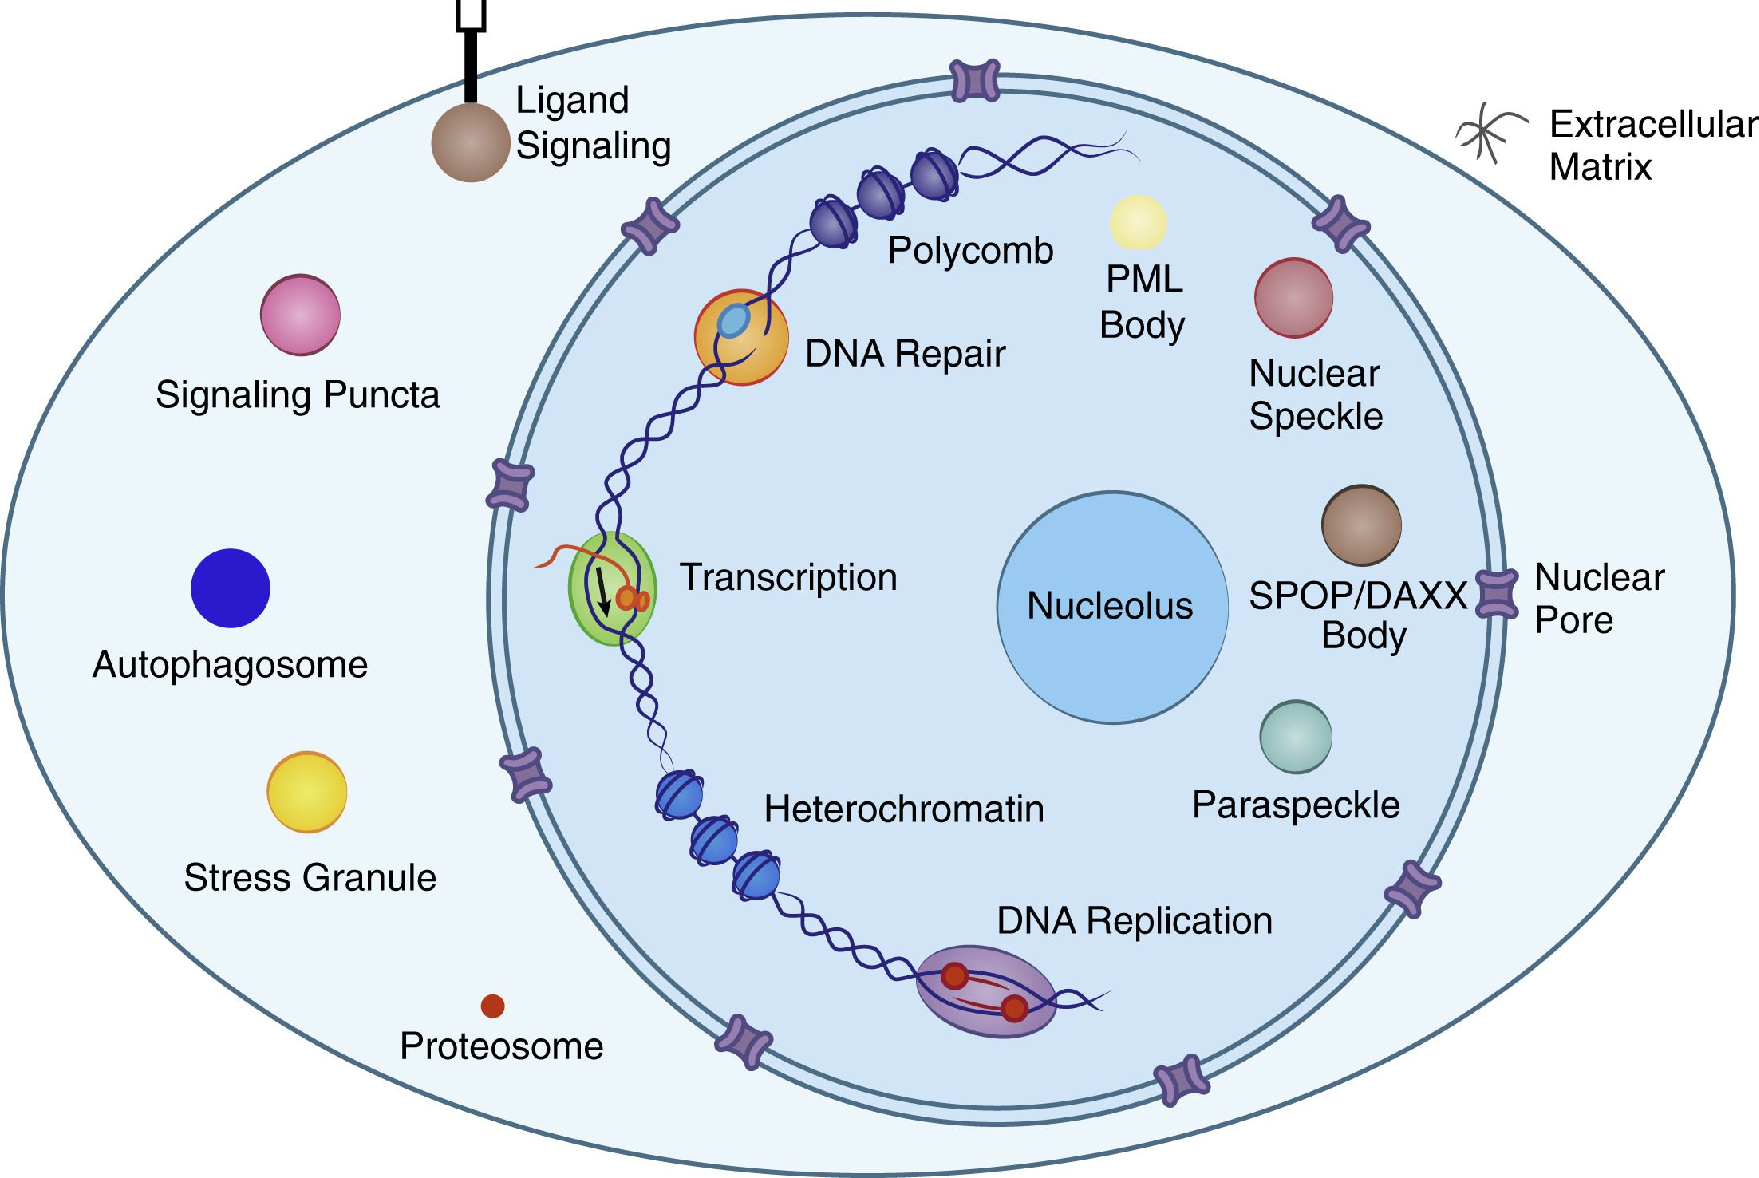
\includegraphics[scale=0.4]{MainContent/BioFigures/basic_image.pdf}
\caption{\textbf{Schematic showing the complex intracellular environment of the cell.}
Figure shows various membrane-bound and membrane-less organelles scattered throughout the cytoplasm inside the cell.
Reprinted with permission from Boija et al. \cite{Boija2021} under License number 5287881024090.
}
\label{fig:basic_image}
\end{figure}
For fulfilling it's many functions, the cell needs to spatially and temporally organize it's interior, consisting of macromolecules such as DNA and RNA, in an energetically efficient and fast manner.
This is an incredibly difficult task, as every second, thousands of biomolecular reactions happen inside the cell; see Ref. \cite{Flamholz2014}, of which a large fraction happens in aqueous mediums, see Ref. \cite{Mitrea2016}.

One way this is achieved is through utilizing membrane-bound organelles; see \figref{fig:basic_image}, which provide a physical barrier and act as a `sieve' for proteins and macromolecules entering from the intracellular environment.
For example, the ER and Golgi apparatus efficiently promote protein sorting and Mitochondria provide energy in form of ATP.
However, with the onset of advanced imaging technologies such as the Electron Microscope and techniques such as light microscopy, it has became clear that the intracellular environment also contains membrane-less organelles, also known as biomolecular condensates. 

\section{Biomolecular condensates}

In the last decade, much attention has been devoted to the formation of these aggregates.
The key reason for their formation is believed to be Liquid-liquid phase separation; see Refs. \cite{FloryBook,Keating2021}, which is the phenomena where molecules possessing certain physical or chemical properties aggregate (consisting of various proteins and macromolecules) and phase separate from the rest of the intracellular environment, similar to polymer condensation; see Ref. \cite{Hyman2014}.
For example, membrane-less organelles (or condensates) called P granules were observed in early stage \textit{C. elegans} worm embryos by Brangwynne et al. \cite{Brangwynne2009}, which played a key role in establishing the anterior-posterior axis for the embryos.
% \begin{figure}[t]
% \centering
% \includegraphics[scale=0.53]{MainContent/BioFigures/history.pdf}
% \caption{\textbf{Timeline of development of Liquid-liquid phase separation in biological cells}.
% Figure shows relevant milestones in the development of Liquid-liquid phase separation in the context of biological cells
% Image taken from Wang et al. \cite{Wang2021}.
% }
% \label{fig:history}
% \end{figure}
These condensates are diverse in their appearances and shapes; see \figref{fig:condensates_diverse}, possess complexity in their composition, have multi-layered structures and can have sizes ranging from nanometers; see Ref. \cite{Sabari2018}, upto micrometers; see Ref. \cite{Feric2013}.
\begin{figure}[tb]
\centering
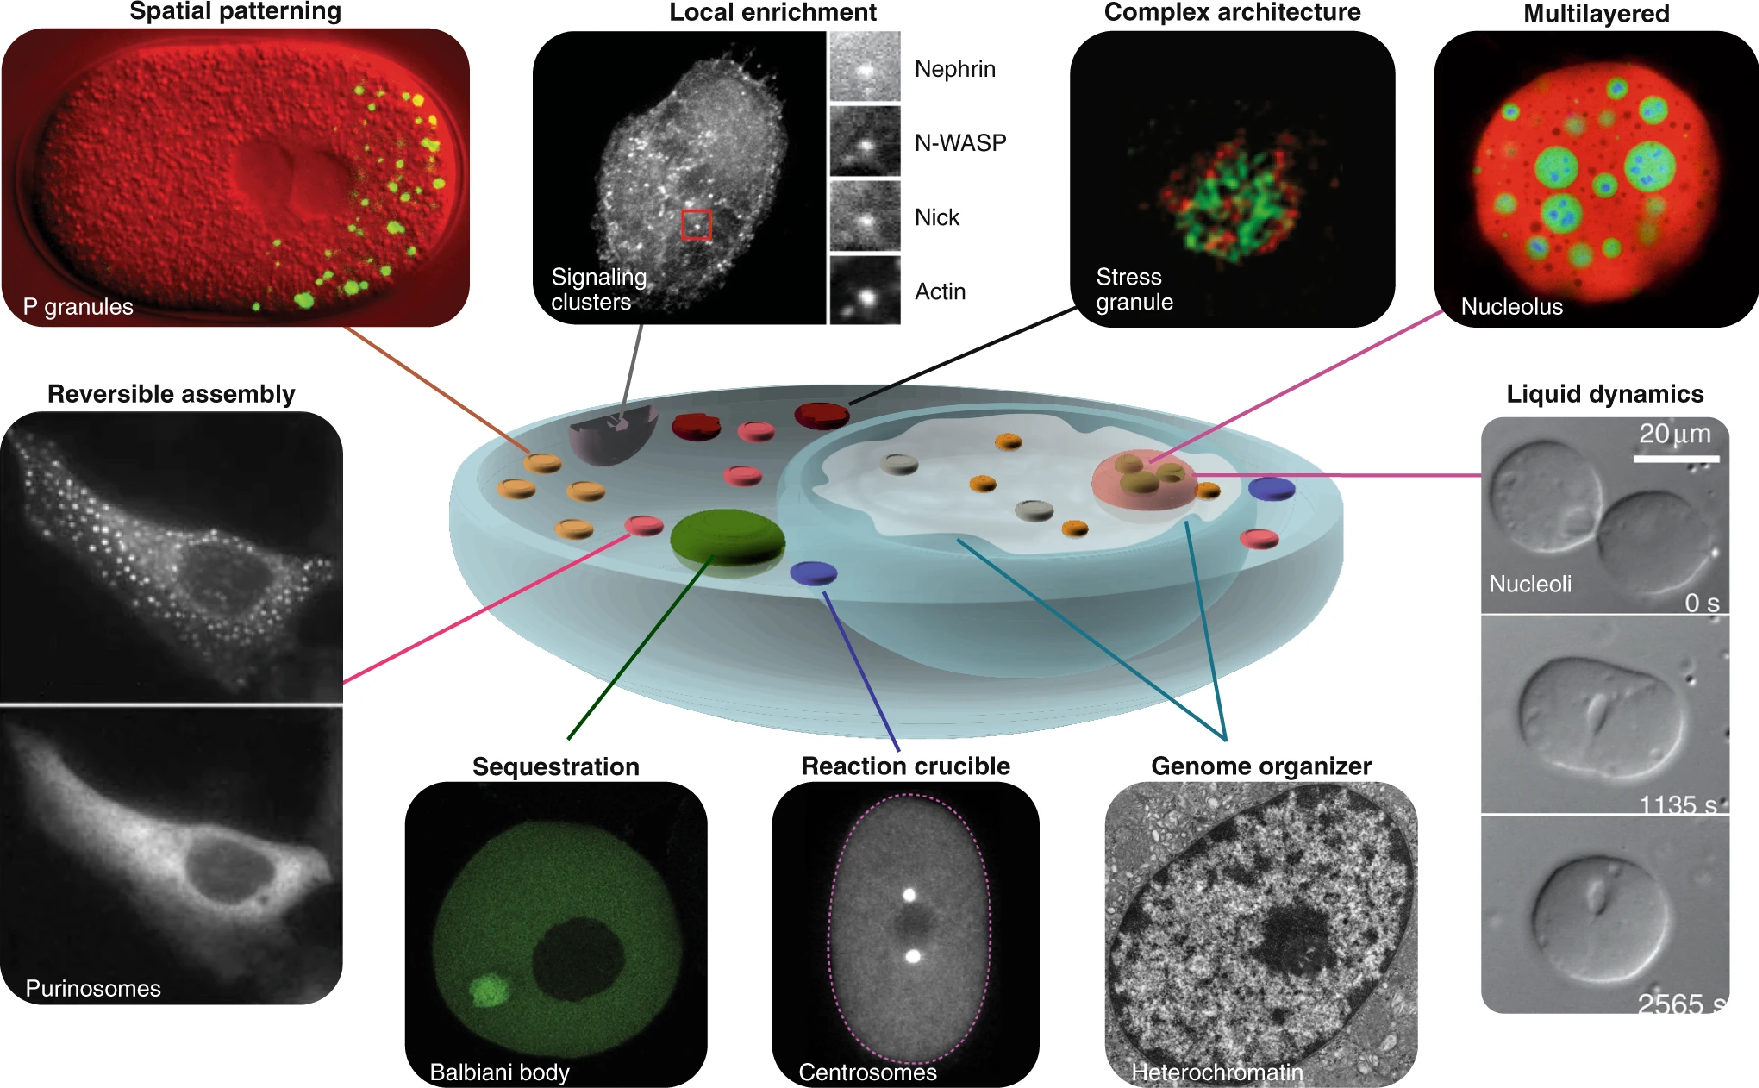
\includegraphics[scale=0.52]{MainContent/BioFigures/condensates_in_cells.pdf}
\caption{\textbf{Membrane-less organelles appear in diverse forms inside the cell.}
Membrane-less organelles (or condensates) possess diverse forms inside the cell and fulfil various functions, as seen from the schematic of the cell in the centre.
Reprinted with permission from Bracha et al. \cite{Bracha2019} under License number 5287590488572.
}
\label{fig:condensates_diverse}
\end{figure}

\section{Condensates are often liquid-like droplets}

Since these condensates form via Liquid-liquid phase separation, these condensates often possess qualities similar to liquid droplets; see \figref{fig:liquid_droplet}.
For example, it was shown by Brangwynne et al. \cite{Brangwynne2009} and Kroschwald et al. \cite{Kroschwald2015} that condensates: are spherical in shape, exhibit coalescence events, fuse with other condensates and form spherical droplets, deform and flow when encountering physical obstacles and regain their shape upon removal of the barrier.
Additionally condensates exchange material with the surroundings via diffusion; see Ref. \cite{Hubatsch2021}, and exhibit wetting phenomena as well; see Ref. \cite{Setru2021}.

\begin{figure}[tb]
\centering
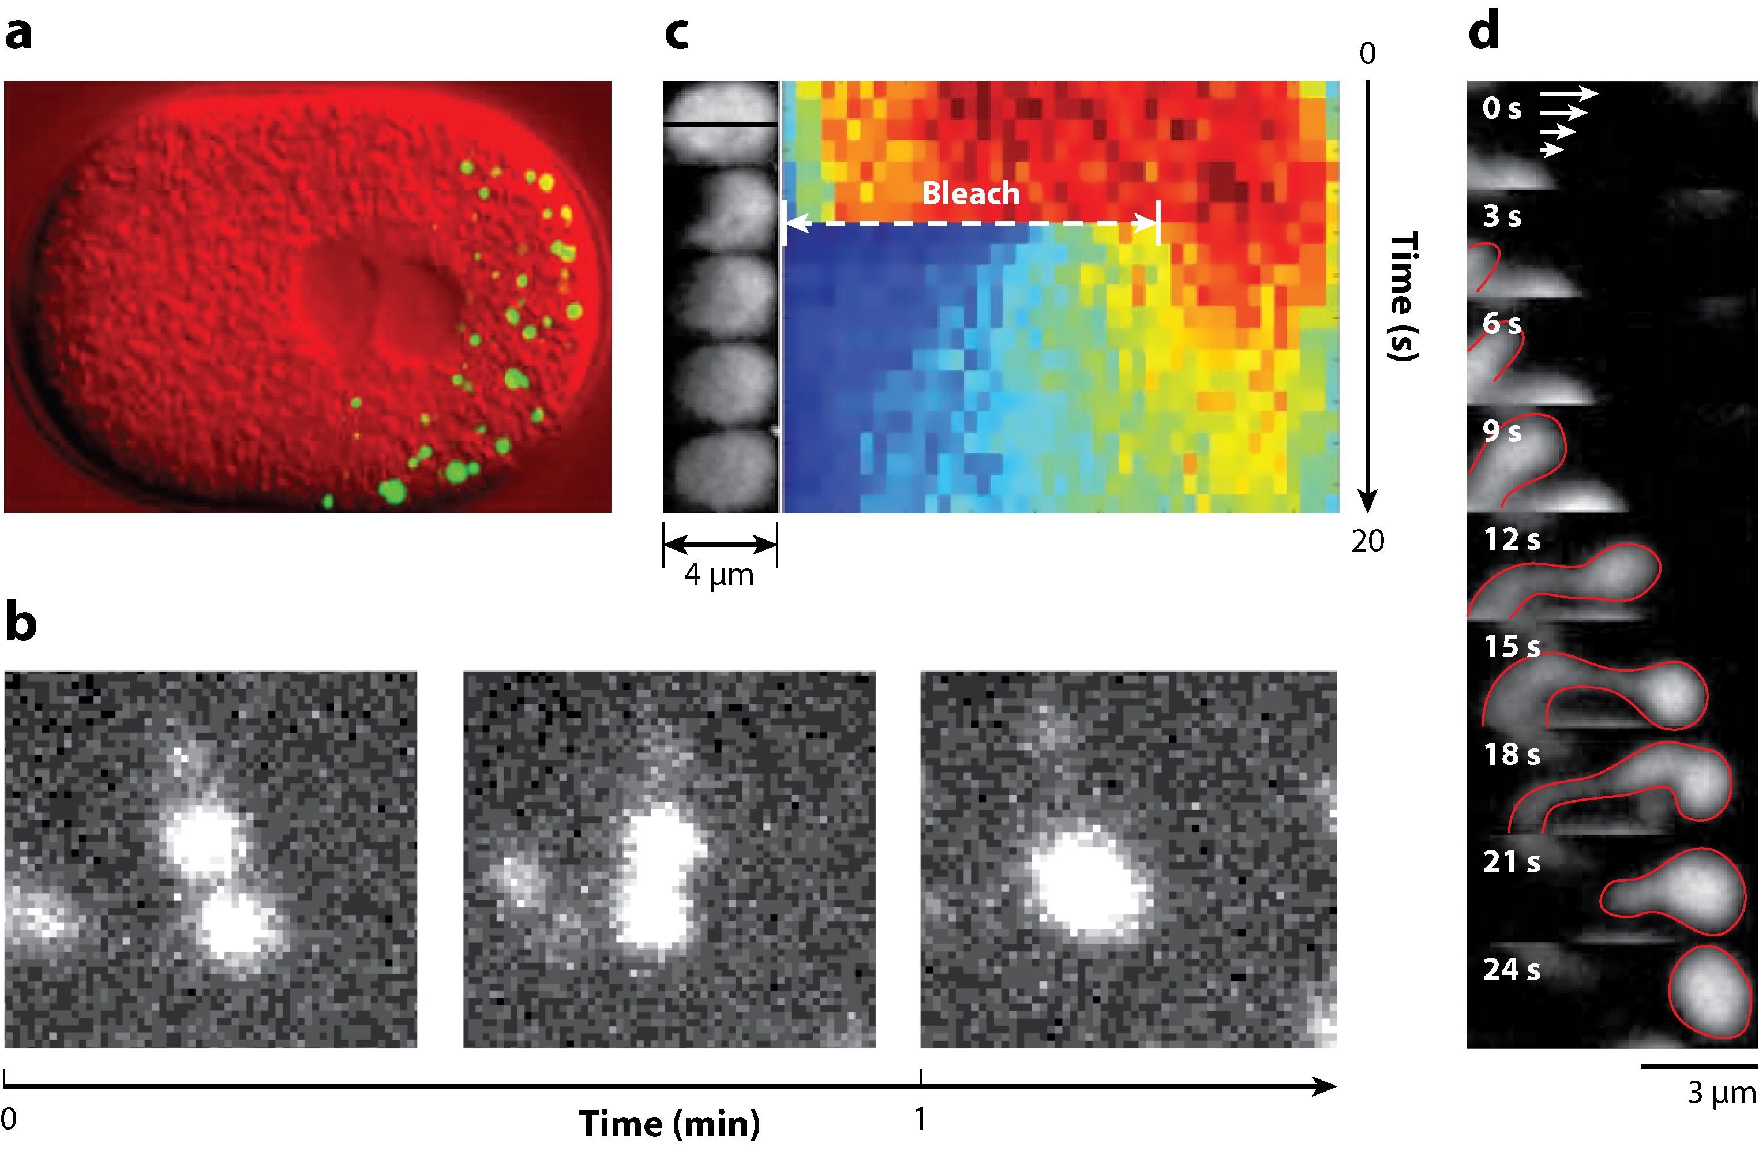
\includegraphics[scale=0.5]{MainContent/BioFigures/liquid_droplet.pdf}
\caption{\textbf{P granules are liquid droplets inside \textit{C.elegans} embryos}
(A) P granules localize to the posterior side of the early stage \textit{C.elegans} embryo.
(B) Two P granules fuse and assume a spherical shape, similar to liquid droplets in minutes.
(C) Photobleaching of half a P granule shows fluorescence recovery in seconds along with kymograph of linear intensity along the black line with red and blue indicating high and background intensity respectively. 
(D) P granules deform in shear flow.
Reprinted from Hyman et al. \cite{Hyman2014} and slightly modified with permission from the publisher with License number 1210872-1.}
\label{fig:liquid_droplet}
\end{figure}

However, not all condensates are liquid-like droplets.
Their structures and architectures can also differ, from being purely liquid-like to gel-like aggregates; see \figref{fig:architecture}.
In particular, condensates can have a liquid or solid shell enclosing a liquid core; see \figref{fig:architecture}A, see \figref{fig:architecture}B and see \figref{fig:architecture}C.
Examples of such condensates can be found in Refs. \cite{JAIN2016487,Putnam2019}.
Condensates can also form `nested droplets'; see \figref{fig:architecture}F, where nucleolus forms such an architecture; see Ref. \cite{Feric2013}.
Each of the sub droplets show liquid-like characteristics and are immiscible as a result of different viscosities. 
Although not common, condensates can also be non-spherical and form a network like assembly; see Ref. \cite{MA20181492} and \figref{fig:architecture}G.
They can even transition from a liquid droplet to a gel-like entity; see Ref. \cite{BOKE2016637} and \figref{fig:architecture}H, and can exhibit viscoelastic properties as well; see Ref. \cite{Jawerth2018}.
\begin{figure}[tb]
\centering
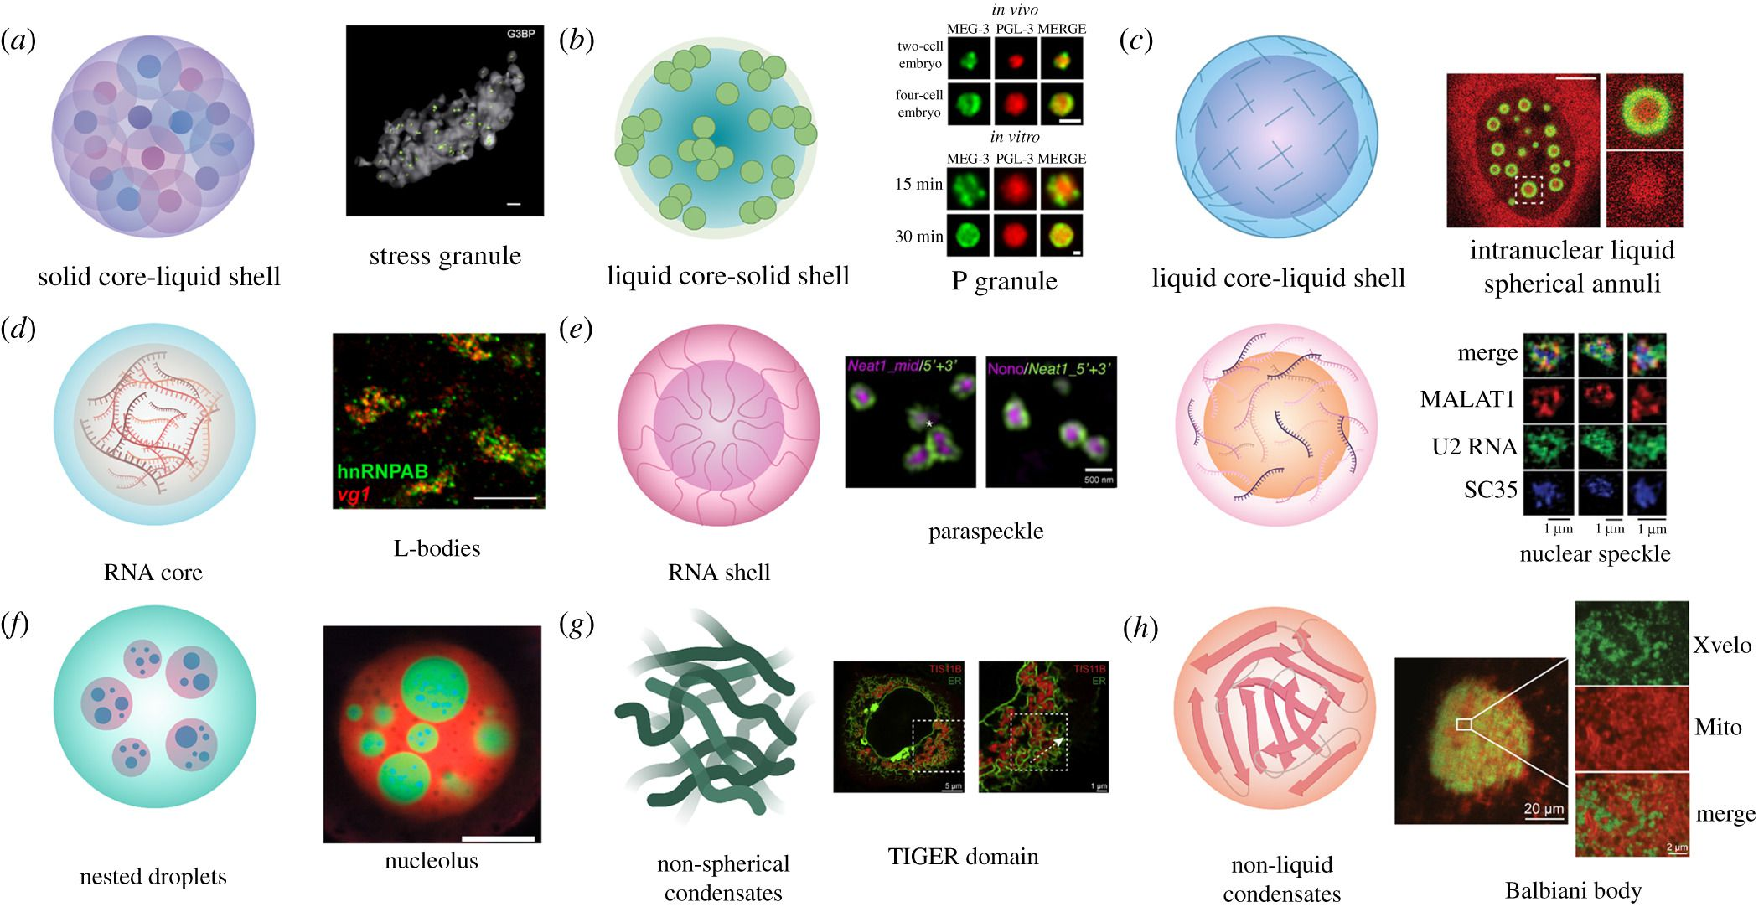
\includegraphics[scale=0.53]{MainContent/BioFigures/architecture.pdf}
\caption{\textbf{Collection of a few condensate architectures.}
Figure depicts collection of diverse architectures for biomolecular condensates ranging from liquid like droplets to gel-like structures. 
Reprinted with permission from Fare et al. \cite{Fare2021} under the Creative Commons Attribution License.
}
\label{fig:architecture}
\end{figure}
Having discussed the diverse architecture possible for condensates, we next discuss the important question: what purpose do they serve?

\section{Condensate function}

Biomolecular condensates have been found to be essential for a wide range of functions, a few being: rearranging molecules to facilitate RNA metabolism and stress signalling, but their precise role is still not well understood.
These functions exist across a wide range of length-scales as well: from molecular scale (for example, augmentation or suppression of chemical reaction rates, controlling folding dynamics of proteins) to the scale of the cell itself (for example, recruiting proteins to specific locations).
We discuss these functions from the context of length-scales.

\subsection{Functions on a molecular scale}

On the molecular scale, condensate formation can: a) Augment or inhibit reaction rates simply as a consequence of increased concentration of the reactants inside; see Refs. \cite{ANDERSSON2008275,Mingjian2018}, and b) Offer reaction specificity by selectively enhancing the functioning of certain biomolecules; see Ref. \cite{Peeples2020}.
Subsequently, condensates can alter local reaction rates and concentration of certain molecules.
They also play a role in regulating nucleation-dependant processes as well, which is evident in the accelerated nucleation of microtubules; see Refs. \cite{Huang2017,King2020}.

On the other hand, condensates can aid in suppression of reactions and decrease overall activity, which is achieved by isolating certain molecules from their regions of interactions or activity; see Refs. \cite{Hirose2014,POWERS2019177}.
Additionally, condensates like the nucleolus are thought to play a key role in prevention of misfolded protein aggregates when the cell encounters a sudden stress event.
Upon heat shock, certain thermally unstable proteins (which are prone to aggregation upon stress) are known to migrate in the nucleolus (so they do not aggregate), and are released back after the shock subsides; see Ref. \cite{Frottin2019}.

\subsection{Functions on the cellular scale}

On the cellular scale, condensates can recruit and concentrate cellular materials to distinct locations within the cell.
Consequently, size presents a big hurdle for the cell to compartmentalize it's interior and a clear correlation has been observed with cell size and aberrant condensate formation.
One way the cell alleviates this problem is by forming different condensates and optimizing their functions accordingly; see Refs. \cite{LEE2013572,Lee2015}, thus exhibiting the importance of spatiotemporal regulation of condensates by the cell.

However, large cells such as neurons, oocytes and muscle cells still must spend additional energy to spatially organize their interior, as compared to smaller cells.
In particular, transport of RNA-protein condensates in neurons is essential for neuron functioning; see Refs. \cite{LIAO2019147,KANAI2004513}.
These condensates are utilized to transport mRNA molecules efficiently over large distance in neurons (which can often be several metres in length; see Ref. \cite{Ishizuka1995}).
Failure to do so promotes formation of aberrant RNA-protein condensates, which can potentially cause diseases such as amyotrophic lateral sclerosis; see Ref. \cite{Altman2021}.
Condensates can also function as storage bins, which can stock up RNA and proteins throughout multiple divisions, for example the RNA binding protein FMR1 is thought to implement this function in oocytes; see Ref. \cite{Greenblatt2018}.
This storage is advantageous to cells who do not undergo frequent cell division, as frequent division can potentially dilute condensate compositions.

Cells might also employ condensates to passively buffer stochastic noise, known as gene expression noise; see Refs. \cite{Eldar2010,Klosin2020}.
Furthermore, as the physics of phase separation is sensitive to conditions such as temperature and pH; see Ref. \cite{RUFF2018,}, cells may have evolved mechanism to utilize this sensitivity to serve as a signal to sense changes in the environment.
In particular, certain mRNA proteins rapidly condense in yeast cells in response to a heat stress event as well as in response to an acidification of it's cytoplasm, thereby potentially acting as a heat sensing switch; see Refs. \cite{Bizzarri2008,Orij2011,Munder2016}.

Taken together, there are still a lot of open questions about how condensates form and their precise roles.
Additionally, it is also unclear how the cell manages to control the formation, disassembly and regulate their size and shape both in location and time, which we discuss next.

\section{Spatiotemporal regulation of condensates}

From the previous section, spatiotemporal regulation of condensates plays a big role in proper functioning of the cell. 
Since many of these condensates are liquid-like droplets, a plethora of questions come to mind: 
\begin{enumerate}

    \item How is size and shape of such condensates maintained throughout the cell?
    
    
    \item How does the cell manage to control the precise timing and location of condensate dissolution and formation?
    
    \item How do such condensates remain dispersed as an emulsion in the complex environment of the cytoplasm and not coarsen into one big aggregate?

\end{enumerate}
Various mechanisms have been proposed till date including chemical reactions, chemical gradients, pH and temperature regulation, physical barriers which prevent droplet-droplet coarsening, usage of Pickering agents to slow down condensate dynamics and ripening, transformation into gel-like structures to preserve certain functions and so on.
We touch upon a few of the mechanisms by which the cell is potentially thought to
control formation, location and size of biomolecular condensates; while simultaneously discussing the implications of poor spatiotemporal control over condensate dynamics as well.

\subsection{Chemical gradients}

The cell can also utilize chemical gradients throughout it's cytoplasm to spatially organize intracellular condensates which plays an important role during the asymmetric cell division. 
In the pioneering work by Brangwynne et al. \cite{Brangwynne2009}, they investigated P granules in early stage embryos of \textit{C. elegans}.
Prior to the first division, P granules are evenly distributed in the cell.
As time passes, they localize to the posterior side of the cell, thus creating the anterior-posterior axis of the cell; see \figref{fig:gradient_change}A. 
This localization was shown to be facilitated by gradient of MEX-5 (which is an RNA-binding protein), arising out of different phosphorylation rates of MEX-5 along the anterior-posterior axis of the cell; see Refs. \cite{Griffin2011,Benelli_2020,Wu2018}.

\begin{figure}[tb]
\centering
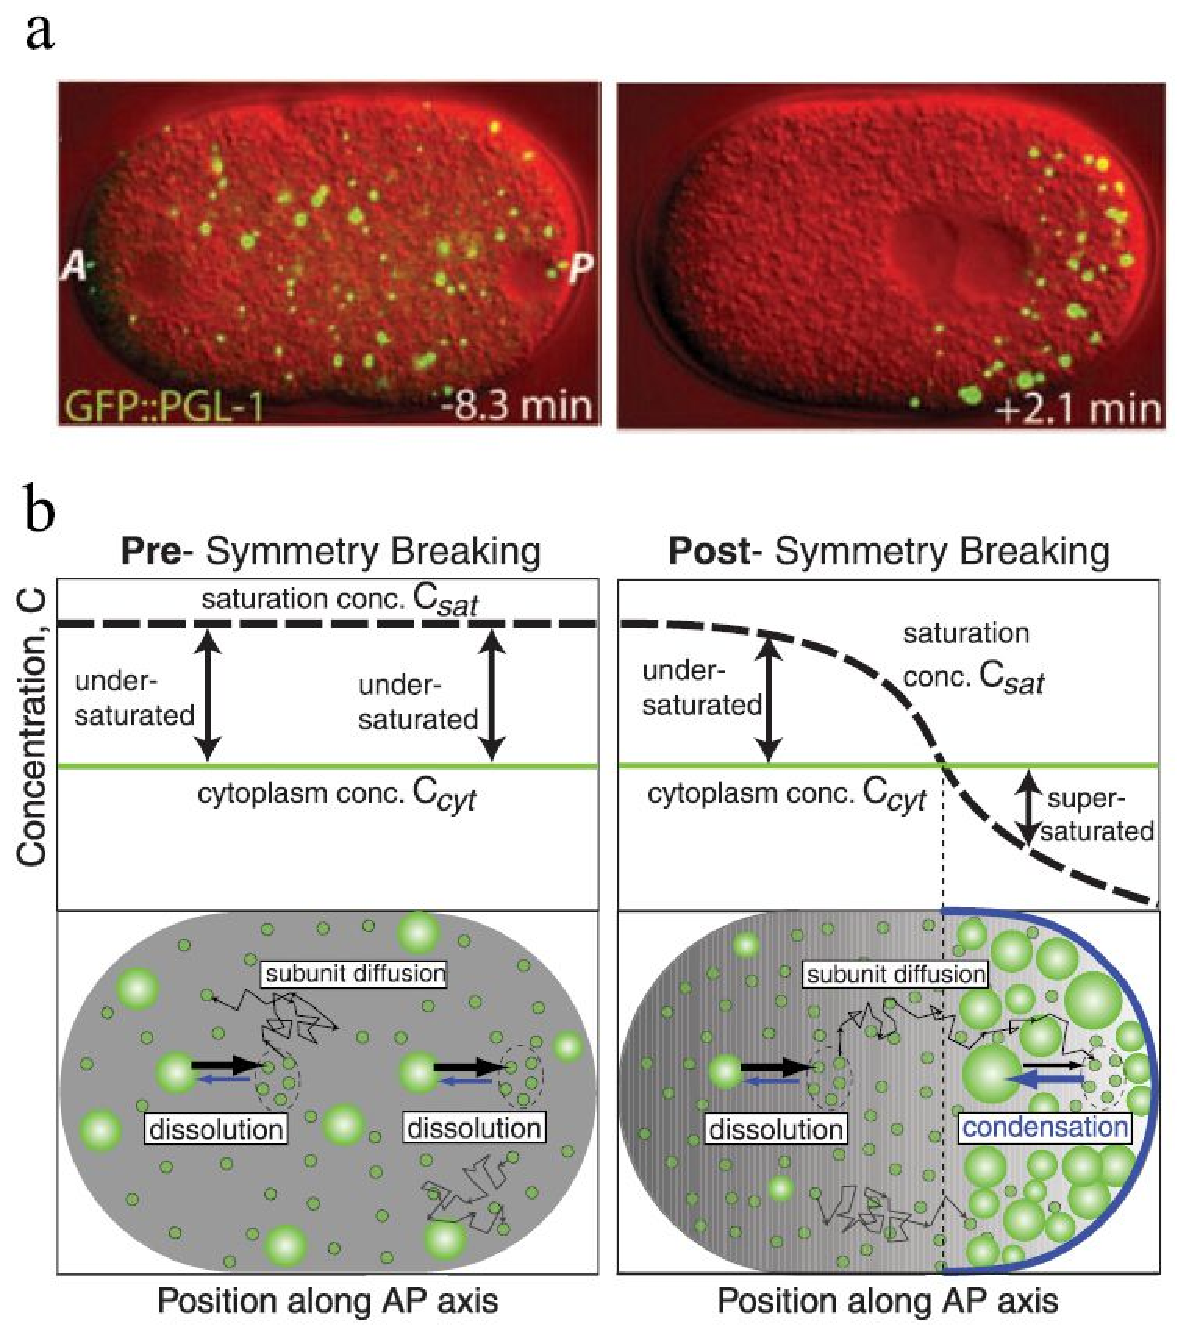
\includegraphics[scale=0.5]{MainContent/BioFigures/gradient.pdf}
\caption{\textbf{Segregation of P granules in early \textit{C. elegans} embryo.}
(A) Initially well mixed P granules (in green) migrate from the anterior to the posterior side of the cell, prior to the first cell division.
Time measured relative to the meeting of two pro-nuclei.
(B) Spatially dependant saturation concentration is established along the anterior-posterior axis, leading to droplet growth on the posterior side and dissolution events on the anterior side. 
Reprinted from Berry et al. \cite{Berry2018} and slightly modified with permission from the publisher with License number 1210876-1.
}
\label{fig:gradient_change}
\end{figure}

Furthermore, it was also shown that the primary mechanism behind localization of P granules was a spatially dependant demixing concentration along the anterior-posterior axis; see \figref{fig:gradient_change}B.
This led to formation and growth of the granules at the posterior side and dissolution events at the anterior side.
Consequently, localization of P granules was anti-correlated with the MEX-5 gradient.

\subsection{Chemical reactions}

After phase separation induces the formation of biomolecular condensates, the cell now has to actively tune condensate properties, so they do not coalesce and clump into one single aggregate.
It is very likely that cells utilize active processes to regulate the function and structure of these condensates, such as: a) Utilizing molecular chaperones and b) Enzymes that facilitate post translational modifications (PTMs) of proteins.
We will mainly focus on these two broad sub-types of active processes in this chapter and discuss them next. 

\subsubsection{Molecular chaperones}

Molecular chaperones are proteins which convert energy into reformulating protein-protein interactions; see Refs. \cite{Akerfelt2010,Tyedmers2010}, and are known to control dynamics, structural properties (for example, increasing porosity of condensates to enhance material exchanges) and stability of stress granules when inducing and removing stress.

Jain et al. \cite{JAIN2016487} investigated in vivo the structural properties of stress granules (which encompass a dynamic shell with a stable core; see \figref{fig:architecture}).
Interactions of the core and the shell (and thus the stability of stress granules) were shown to be modulated by a chaperone TRiC/CCT, which also was identified as a key component of stress granules.
Similarly, Mateju et al. \cite{Mateju2017} identified the role of chaperones named HSP70 in preventing the formation of aberrant stress granules (containing misfolded proteins), which are thought to be the key culprits in diseases such as amyotrophic lateral sclerosis (ALS) in human cells.
Furthermore, HSP70 also aides the dissolution of these stress granules when stress is removed; also see Ref. \cite{Wallace2015}, thereby showing that chaperones can act as quality control managers to prevent aggregation of misfolded proteins, and preserving the dynamics of stress granules. 

Additionally, Qamar et al. \cite{QAMAR2018720} showed that a chaperone called transportin regulates FUS (FUused in Sarcoma - an RNA binding protein) condensation and phase separation in neuron terminals; see Ref. \cite{Chen2019}, and is important for preventing diseases such as familial amyotrophic lateral sclerosis (fALS) and frontotemporal lobar degeneration (FTLD).

\subsubsection{Post-Translational Modifications of proteins}

PTMs of proteins are also considered as a key regulating mechanism of the dynamics and structure of condensates, which function by adding key functional groups to proteins, thus modifying their interactions with other biomolecules.

Hofweber et al. \cite{Hofweber2019} investigated the role of PTMs of RBPs (RNA-binding proteins) in regulating the dynamics of Ribonucleoprotein (RNP) granules, which are condensates consisting of RBPs and RNA.
Weak interactions between RBPs and RNA are responsible for phase separation, which are reduced by slow Arginine methylation (a type of PTM) of RBPs, thereby almost always inhibiting phase separation; see Refs. \cite{QAMAR2018720,Ryan2018,NOTT2015936}.
Arginine methylation of RBPs is thought to regulate RNP granules by two methods - through modifications of protein-protein/RNA interactions and through altering the composition of RBPs throughout the cytoplasm or in the nucleus. 
Interestingly, Arginine methylation is found to both suppress; see Refs. \cite{Dolzhanskayaw2006,Tsai2016}, and facilitate; see Refs. \cite{Matsumoto2012,ArribasLayton2016}, the dynamics and formation of RNP granules.

Contrary to Arginine methylation, Phosphorylation (another type of PTM) is known to be a fast and reversible mechanism and is known to both - suppress; see Refs. \cite{Rhoads2018,Wang2018}, and promote; see Refs. \cite{KAMPERS1996344,Vanderweyde8270}, phase separation. 
Similar to Arginine methylation, Phosphorylation seems to be a key mechanism through which the dynamics, formation and dissolution of RNP granules can be tuned.
Phosphorylation is thought to regulate RNP granules through altering the composition of RBPs by promoting or degrading them, thereby controlling RNP granule formation; see Refs. \cite{Sfakianos2018,MAHBOUBI20151725}, and dissolution; see Refs. \cite{Aranda2011,KRISENKO201527803,Reineke2018}. 
Ambadipudi et al. \cite{Ambadipudi2017} and Wegmann et al. \cite{Wegmann2018} found that Tau phosphorylation changes the charge distribution on the microtubule-binding domain of Tau and enhances electrostatic interactions and promotes phase separation and the growth of Tau droplets.
These droplets are precursors to Tau aggregates, accumulation of which play a role in Alzheimer’s disease; see Refs. \cite{Williams2006,Mucke2009}.

Thus, both - Arginine methylation and Phosphorylation in conjunction, can either promote or inhibit phase separation and dynamics of RNP granules, and thus are good candidates for tuning phase separation and dynamics of RNP granules; also see Refs. \cite{Schisa2021,VelazquezCruz2021}.
Lastly, Glycosylation is another PTM which regulates phase separation. 
In particular, Roth et al. \cite{Roth2017} found for the first time an inverse correlation between Phosphorylation and O-GlcNAcylation in human colon cells in regulating phase separation and inhibiting tau protein condensation. 

Enzymatic reactions can also play a role in the dynamics of condensates. 
In particular Hondele et al. \cite{Hondele2019} found that DEAD-box ATPase family can control formation and dissolution dynamics of RNA condensates in both - prokaryotes and eukaryotes.
They showed that ATPase exists in an ATP-bound state, which promotes phase separation of condensates, and an ATP free state, which accentuates condensate dissolution. 
Utilizing chemical reactions to control droplet growth has also been reviewed recently by S\"{o}ding et al. \cite{SODING20204}, where the authors put forward two important mechanisms - Enrichment inhibition; see Refs. \cite{Wang2014,Kirschbaum2021}, and Localization induction; see Refs. \cite{Langelier2012,Kirschbaum2021}.

These examples clearly highlight that chemical reactions play an important role in tuning the dynamics and stability of condensates. 

\subsection{Regulation of pH and temperature}

pH as a regulatory mechanism for phase separation inside the cell has been studied extensively; see Refs. \cite{Orij2011,Kroschwald2018,Peters2013,Petrovska2014}.
In particular, Bizzari et al. \cite{Bizzarri2008} and Orij et al. \cite{Orij2011} were one of the first to focus on pH as a regulatory mechanism for the cell. 
Orij et al. \cite{Orij2011} focused the yeast species \textit{Saccharomyces cerevisiae} and demonstrated pH as a fast and simple mechanism which the cell uses to spatially organize it's intracellular condensates.

Munder et al. \cite{Munder2016} in their seminal work, investigated how eukaryotic cells (budding yeast) regulate pH in their cytoplasm to control the mobility and structual properties of the condensates.
In their natural habitat, yeast cells typically live in acidic environments (pH $\approx 5.5$), but the cytoplasm is kept at a neutral pH in normal circumstances (pH $\approx 7.3$).
However, when faced with nutrition scarcity,
Munder et al. observed that upon acidification, the cytoplasm transitions reversibly from liquid-like to gel-like structure; see \figref{fig:pH_change}.
\begin{figure}[tb]
\centering
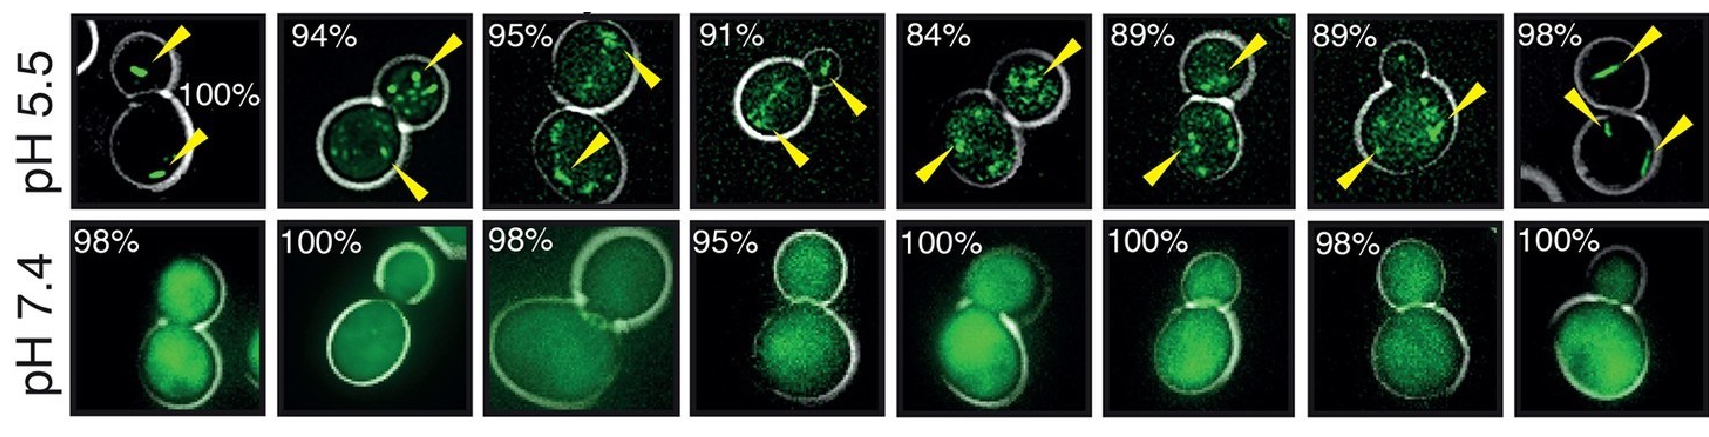
\includegraphics[scale=0.53]{MainContent/BioFigures/ph_change.pdf}
\caption{\textbf{Acidification of cytoplasm induces aggregation of proteins into structures.}
Proteins aggregate into structures depending on cytosolic pH.
When pH is lowered from 7.4 (middle row) to 5.5 (top row), proteins assemble into structures (green dots, top row) and help the transition of the cytoplasm from a liquid-like to a gel-like entity.
These structures were absent and proteins are well mixed when the cytoplasm was almost pH neutral (bottom row), but present when the cytoplasm becomes acidic (top row).
Reprinted with permission from Munder et al. \cite{Munder2016} and slightly modified under the Creative Commons Attribution License.
}
\label{fig:pH_change}
\end{figure}
The transition, which is facilitated through many proteins forming peculiar structures upon a change in cytosolic acidity, is functionally important, as when the cytoplasm is not allowed to solidify, the yeast cells simply die.

Organisms can also regulate phase separation utilizing temperature as a control parameter.
For example, the effect of cyclical variations in temperature on the dissolution and reformation of P-granules in early embryos of the \textit{C. elegans} worm was studied by Fritsch et al. \cite{Fritsch2021}, in agreement with earlier works by Putnam et al. \cite{Putnam2019} and \cite{Andresphdthesis2016}, who investigated mixing and de-mixing of P-granules from the cytoplasm.
Fritsch et al. \cite{Fritsch2021} demonstrated through constructing in vivo phase diagrams that physics of phase separation adequately explains this dynamic process of dissolution and reformation of P-granules, which is dictated by local thermodynamic equilibrium.
The P-granules undergo dissolution upon increasing the temperature and their reformation is recovered upon cooling, thus showing that temperature can be a control mechanism that the organism uses to control stability and dynamics of the condensates.

% \figref{fig:temperature_change}A shows the schematic of an early stage embryo of the \textit{C. elegans} worm and the zoomed in view of the embryo studied. 
% As seen from \figref{fig:temperature_change}B, 

Temperature as a control parameter also appears in plants, for example, Zhu et al. \cite{Zhu2022} investigated the link between stress tolerance, temperature and phase separation in \textit{Arabidopsis thaliana} (a model organism in plant based studies) and showed in vivo that RNA-binding proteins called RBGD2 and RBGD4 condense upon increase in temperature, thus improving heat resistance.
Apart from these thermodynamic properties, physical properties of the intracellular environment can also influence condensates, which we discuss next. 
% \begin{figure}[tb]
% \centering
% \includegraphics[scale=0.65]{MainContent/BioFigures/temperature.pdf}
% \caption{\textbf{Effect of temperature on dissolution and formation of P-granules.}
% (A) shows a schematic of an early stage embryo of the \textit{C. elegans} worm and the zoomed in view of the embryo studied with P-granules in yellow. 
% (B) shows P-granules (yellow green dots) undergo cyclical dissolution and reformation subjected to alternating temperatures. 
% Image taken from Fritsch Anatol W., Diaz-Delgadillo Andrés F., Adame-Arana Omar, Hoege Carsten, Mittasch Matthäus, Kreysing Moritz, … Weber Christoph A. (2021). Local thermodynamics govern formation and dissolution of Caenorhabditis elegans P granule condensates. Proceedings of the National Academy of Sciences, 118(37), e2102772118. doi:10.1073/pnas.2102772118.
% }
% \label{fig:temperature_change}
% \end{figure}

\subsection{Physical modifications of intracellular environment}

Inside the crowded environment of the cell; see Ref. \cite{Andre2020}, dynamics of biomolecular condensates are coupled with the dynamical properties of the cytoskeletal filaments, and can thus influence each other's size, shape and structural properties; see \figref{fig:mechanical_forces_in_cells}.
We will discuss some important studies which highlight how the cytoskeletal networks affects the spatiotemporal dynamics of condensates. 

\begin{figure}[tb]
\centering
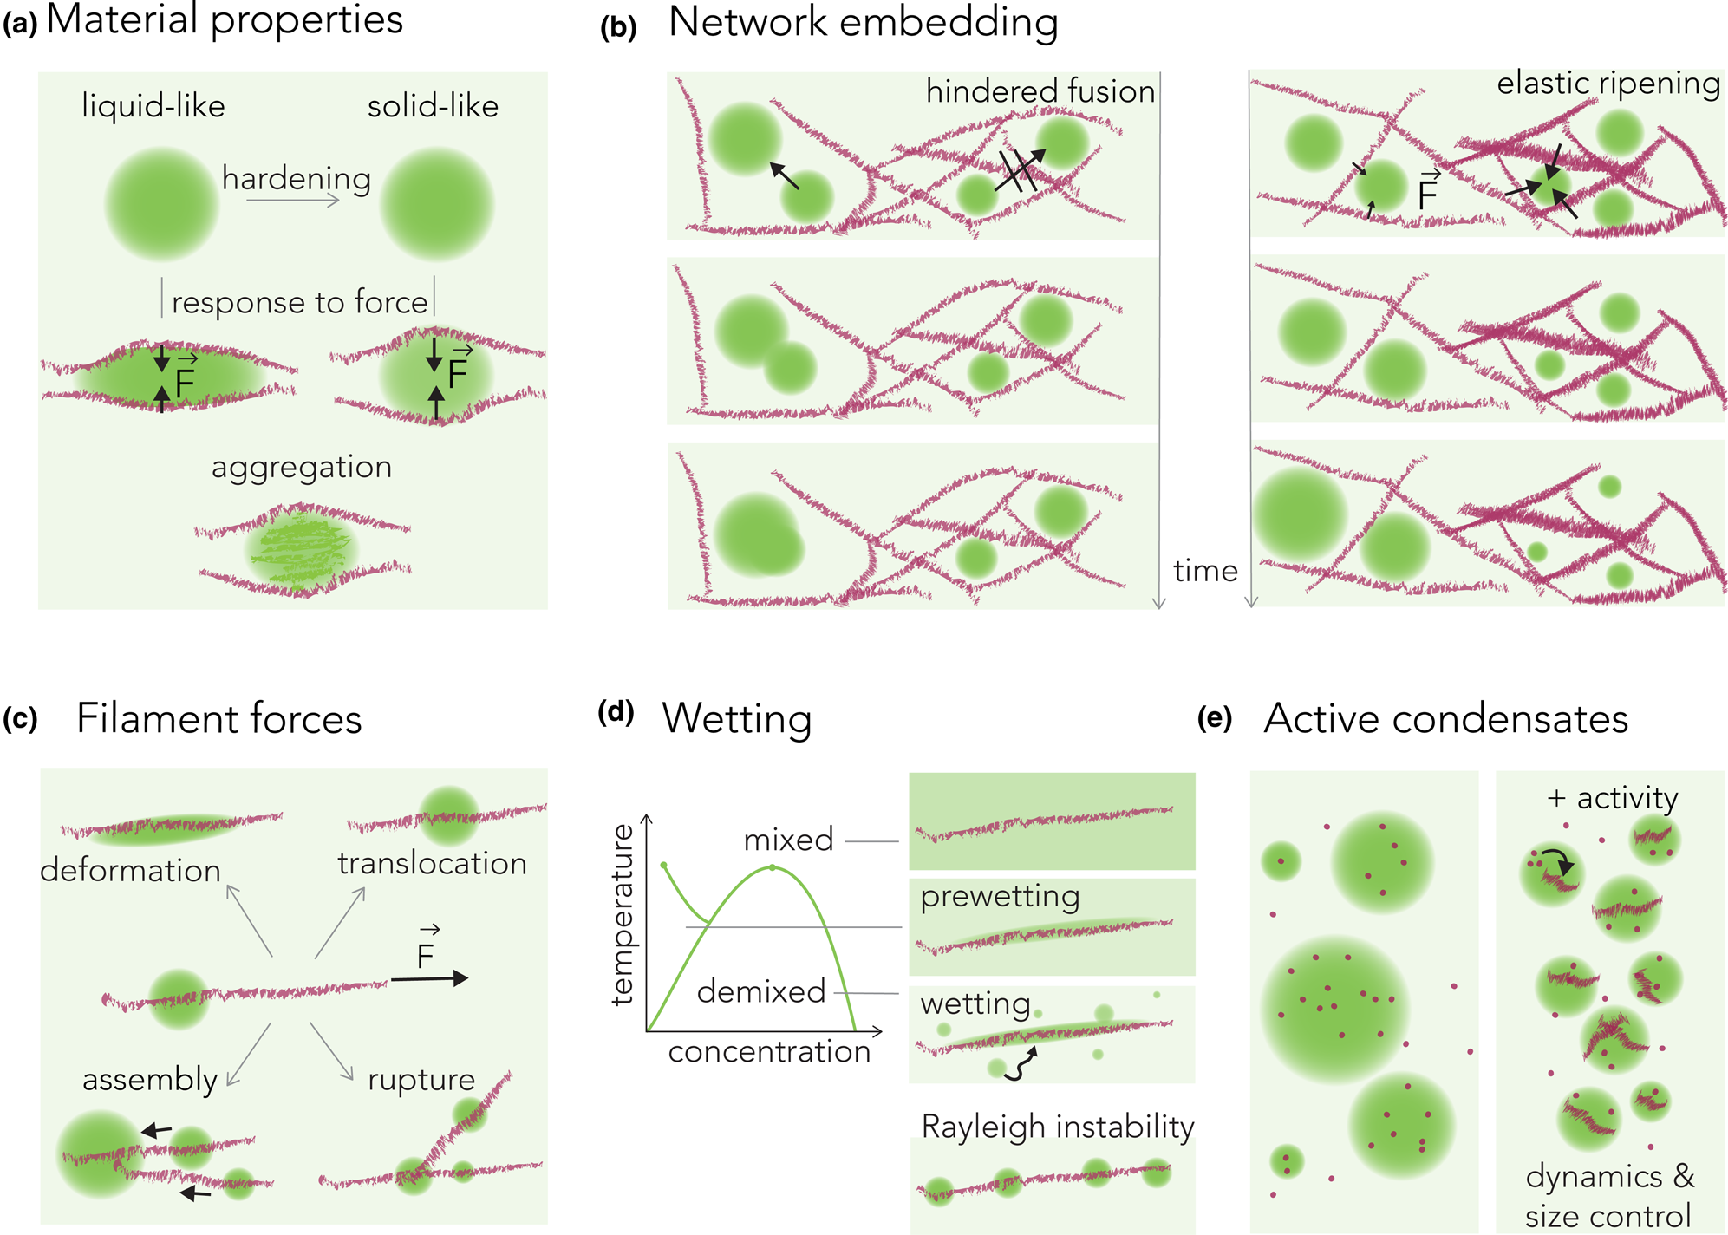
\includegraphics[scale=0.53]{MainContent/BioFigures/scaffolds.pdf}
\caption{\textbf{Cytoskeletal networks influence the stability and dynamics of condensates.}
(A) Cytoskeletal filaments influence condensate stability by exerting physical forces; see Ref. \cite{Enos2018}.
(B) Cytoskeletal networks can stabilize large condensates through mechanical forces and act as a `condensate sieve';  see Ref. \cite{Quiroz2020}.
Heterogenous elastic networks can reverse \textit{Ostwald-Ripening} and stabilize small droplets; see Refs. \cite{Rosowski2020,D0SM00628A}.
(C) Contracting or extending networks can control droplet dynamics; see Ref. \cite{Enos2018}.
(D) Wetting phenomena can also influence and drive phase separation; see Ref. \cite{Setru2021}.
(E) Active processes can stabilize emulsions of many droplets; see Refs. \cite{Zwicker2015,Review2019}.
Reprinted from Wiegand et al. \cite{Wiegand2020} with permission from the publisher with License number 1210880-1.
}
\label{fig:mechanical_forces_in_cells}
\end{figure}

Feric et al. \cite{Feric2013} in their pioneering work investigated the role of nuclear actin in Oocytes of the frog \textit{Xenopus laevis}.
They demonstrated the importance of actin mesh in keeping the typically large nucleoli ($\sim 450 \, \mathrm{\mu m}$ in diameter) from coalescing and sedimenting under gravity, thus demonstrating the mechanically stablizing role of actin.
Furthermore actin network also acts as a `condensate sieve', allowing smaller condensates to diffuse while arresting the dynamics of bigger condensates.

Similarly, Enos et al. \cite{Enos2018} showed that Pericentriolar material (PCM - outer layer of centrosomes) dissolution in \textit{C. elegans} embryo is governed by a dephosphorylation process of the scaffolding protein known as SPD-5 and physical pulling forces ripping apart the SPD-5 scaffolding; similar to the schematics in \figref{fig:mechanical_forces_in_cells}A.  More recently, Garcia Quiroz et al. \cite{Quiroz2020} have shown that keratin filament networks in mammalian skin cell layers can stabilize condensates known as keratohyalin granules; see \figref{fig:mechanical_forces_in_cells}B, and keep them from fusing by caging, thus keeping individual condensates apart from each other and maintaining their stability.

B\"{o}ddekker et al. \cite{Boeddeker2022} investigated the interaction between cytoskeletal filaments (microtubules) and condensates (stress granules) to understand the role of viscoelastic environments in controlling phase separation inside U2OS epithelial cells.
In the vicinity of stress granules, microtubule network density is higher and the network is severely deformed.
Polymerization and depolymerization of the microtubules directly affected the surface properties of stress granules, which hints at tuning of networks as a control mechanism for the cell.

The presence of heterogeneous elastic networks can also affect phase separation - in particular, reverse \textit{Ostwald-Ripening} - where large droplets give up material and feed the smaller droplets, as shown by Rosowski et al. \cite{Rosowski2020,D0SM00628A} and Vidal-Henriquez et al. \cite{VidalHenriquez2021}, shedding light on potentially controlling ripening processes by taking advantage of heterogeneous elastic networks inside cells.
There also have been exciting recent advances in exploring the viscoelastic network of chromatin, which exhibits slow coarsening of condensates and retards coalescence.
In particular, Qi et al. \cite{Qi2021} studied condensate coalescence in the presence of chromatin networks using theory and simulations and showed that condensate (nucleoli) - chromatin interactions promoted nucleation, but hindered coalescence.
Similarly, anomalous diffusion of condensates due to physical constraints from the viscoelastic chromatin network was reported by Lee et al. \cite{Lee2021}, where the coarsening exponent was found to be $\beta \sim 0.12$, as opposed to the theoretical prediction of $\beta = 0.33$; see Refs. \cite{Review2019,Weber2017}.

Lastly, wetting phenomena is also responsible to driving phase separation, for example, Jiang et al. \cite{Jiang2015} showed that a protein called BuGZ forms liquid droplets on microtubules.
Similarly, Setru et al. \cite{Setru2021} investigated the dynamics of droplets formed by condensation of a protein called TPX2 on microtubules; see \figref{fig:mechanical_forces_in_cells}D. 
They showed that a fluid instability drives the condensation and TPX2 droplets not only form a one dimensional lattice on the microtubule branch, but the inter-droplet distance increases with increasing TPX2 concentration.
Taken together, all the above examples show the interplay between condensate dynamics and the intracellular environment. 
However, instead of controlling the properties of it's internal environment, the cell can also regulate properties of the condensates themselves, which we discuss next. 

\subsection{Modifying properties of condensates}

Recently, applications from pharmaceutical and food industries, such as the usage of `Pickering agents' in stabilizing emulsions; see review by Yang et al. \cite{Yang2017} and references therein, have inspired similar studies in the context of biological cells.

Pickering agents are solid particles, typically nanoscale sized, which adsorb on the interfaces of liquid droplets with partial wetting. Adsorption is favoured energetically, thereby reducing the affinity of the droplets towards lowering their surface area, leading to slowing down of their coarsening.
The discuss a few studies which suggest that cells may recruit biopolymers (which are plenty in the cytoplasm; see Ref. \cite{Burla2019}), as Pickering agents.
This is exciting as it could provide an additional pathway for the cell to as an organizing principle for intracellular biomolecular condensates.

Folkmann et al. \cite{Folkmann2021} studied and investigated mechanisms responsible for anomalous coarsening of P granules (which are made up of RNA and a protein called PGL-3) in \textit{C. elegans} when transitioning from egg to embryo.
Earlier studies by Putnam et al. \cite{Putnam2019} have shown that an intrinsically disordered protein called MEG-3 stabilizes PGL-3 droplets by forming a scaffold around them, thus spatially regulating their condensation in the cytoplasm.
Folkmann et al. then identified MEG-3 clusters as a Pickering agents inside the cell, which adsorb to the interface of P granules and pose as a physical obstacle, slowing down their coarsening.

Similarly, Zhang et al. \cite{Zhang2018} suggested that EPG-2 clusters act in a similar way as MEG-3 to regulate the dynamics of PGL droplets.
EPG-2 accelerates the transition of PGL-1/3 droplets into gel-like structures, rendering them less dynamic and more stable.
Lastly, Tauber et al. \cite{Tauber2020} also suggested a similar adsorption mechanism, indicating that mRNAs aggregating on the surface of protein condensates may act as stabilizing agents.

All the above examples clearly exhibit the complex coupling between the condensate dynamics and dense networks, suggesting cells can tune the network properties in their interior to exert spatiotemporal control over formation, stability and dynamics of the condensates. 

Computational and theoretical models can help unravel the coupling of condensates and the intracellular environment and mechanisms of spatiotemporal control by the cell.
Computational models are generally useful, as exploring large parameter spaces is not a limitation, relative to experimental studies.
Additionally, studying the effects of control parameters on long time and length-scales is an advantage for computational models.
We next discuss some computational and theoretical approaches used to study phase separation behaviour.

\section{Modelling and simulations of phase separation}

Broadly speaking, computational models fall in two main categories: \textit{Field-based} models and \textit{Particle-based} models.

\subsection{Field-based models}

The field-based models typically have a continuum based approach, where the presence and effects of various biomolecules is represented by changes in the field variables like density or composition $\phi(\vec{x})$.
Then, a general free energy of the system is formulated as a functional of the composition $F[\phi(\vec{x})]$ with an aim of minimizing the free energy, subject to problem specific constraints, using numerical or analytical approaches.
Typically, phase separation will occur when a generic composition field will minimize the free energy functional $F$.
Additionally, such free energy formulations can then be extended to include the effects of multi-component fluids, chemical reactions, fluid flows and model phase separation in polymers as well.

One such field-based model has been typically used to model phase separation; namely the \textit{Cahn-Hilliard} model; see Ref. \cite{CahnHilliardEq}.
For example, the \textit{Cahn-Hilliard} model, along with theoretical models, has been utilized and modified to study phase separation in binary and ternary mixtures.
In particular, Berry et al. \cite{Berry2015} investigated the disassembly and assembly of nucleoli and ENDs (extranucleolar droplets) in \textit{C. elegans} embryos using a modified \textit{Flory-Huggins} theory; see Ref. \cite{FloryBook} for ternary solutions.
Gasior et al. \cite{Gasior2019} used a multi-phase \textit{Cahn-Hilliard} model to study binding and unbinding of different RNA-protein complexes with an aim to understand spatial patterning and it's role in intracellular organization.

The \textit{Cahn-Hilliard} model has also been used to study phase separation in multi-component systems and used to uncover different morphologies and coarsening behaviour by Mao et al. \cite{Mao2019}.
Similarly, Vweza et al. \cite{ijms22136675} investigated the effects of macromolecular crowding on the coarsening dynamics and morphologies of small condensates, shedding light on their growth and stability.
Field-based models have also found applications in the area of polymer phase separation.
In particular, phase separation in block copolymers has been studied by Ren et al. \cite{Ren2001} and by Fredrickson et al. \cite{Fredrickson2002}, where they recovered various morphological structures (cylindrical, lamellar) by using a modified version of the \textit{Cahn-Hilliard-Cook} model.

Field-based models have also been successful in studying effects on long time and length-scales.
In particular, Weber et al. \cite{Review2019,Weber2017} have demonstrated coarsening behaviour and effects of chemical gradients on phase separation. 
Jacobs et al. \cite{Jacobs2021,JACOBS2017683}
studied phase separation in multi-component mixtures and the effect of random interactions in the stability of multiple phases.  
The effects of chemical reactions and elasticity have been simulated using field-based models as well.
For example, Vidal-Henriquez et al. \cite{VidalHenriquez2021} have studied and modelled the effects of elasticity of chromatin network on droplets, which can serve as a base for further theoretical investigations.
Lastly, the effects of chemical reactions on droplet sizes, stability and coarsening behaviour in ternary mixtures was studied by Wurtz et al. \cite{Wurtz2018}.

Taken together, we have summarized a few representative examples where field-based models have been used to investigate phase separation in diverse areas. 
However, these models have restricted application pertaining to phase separation in the cell, as they do not possess the granularity, specificity and the resolution needed to consider specific protein-protein interactions, as the internal composition of the cytoplasm in the cell is composed of hundreds of biomolecules with specific sequences; see Ref. \cite{Burla2019}.
In the following section, we will elaborate on a different type of model, which alleviates some of the drawbacks of the field-based models. 

\subsection{Particle-based models}

Where Field-based models lack, Particle-based models try to fill that void.
Particle-based models essentially aim to represent different phases in a phase separating mixture as an ensemble of particles.
These particles are typically governed by force fields, which takes into account various interactions arising from chemical bonds and long range interactions such as Coulomb interactions.
A significant advantage particle-based models have over field-based models is the ability to take into account correlations across atoms or molecules without being explicitly integrated in the method.
These models are often used in conjunction with experiments and are typically used to extract features and information about phase separation at a molecular level.

Particle-based models fall into different categories as well, some being \textit{Molecular dynamics} simulations, \textit{Coarse-grained} models and \textit{Lattice-based} models.
Although these models overlap quite a bit in their formulation and distinction between them is not always clear, we will consider them separately and elaborate on each of their merits and demerits. 

\subsubsection{Molecular dynamics simulations}

Simulations falling under the broad umbrella of \textit{Molecular dynamics} simulations; proposed by Alder et al. \cite{Alder1959}, typically evolve dynamics of particles in time using numerical integration of Newton's laws of motion.
For example, Chu et al. \cite{Chu2021} investigated the temperature and charge pattern dependence of a chaperone protein called Swc5 on phase separation in biomolecules and role of Swc5 in chromatin formation.
On similar lines, Farr et al. \cite{Farr2021} studied effects of chromatin compaction on nucleosome dynamics.

To study the interplay between long and short range interactions of intrinsically disordered proteins on the stability, structure and dynamics of condensates, Hazra et al. \cite{Hazra2021} used a coarse-grained molecular dynamics simulation model.
A similar model was also utilized by Espinosa et al. \cite{Espinosa2020} to uncover physical principles governing the stability of multi-component condensates and the effects of networks on these condensates.

However, considering that the crowded environment of the biological cell and the presence of hundreds of biomolecules; see Ref. \cite{Ellis2003}, Molecular-dynamics simulations are extremely expensive, and the computational costs scale up quickly when simulating biomolecules on the level of a single atom or molecule in three dimensions.
Furthermore, these simulations lack an important feature, which is relevant in the case of biomolecules - which is their inability to predict rare events like conformational changes in proteins, protein folding and nucleation events like the initial formation of nucleolus; see Ref. \cite{Falahati2016}.
Some of these drawbacks can be eliminated by using \textit{Coarse-grained} models, which we will discuss next. 
\subsubsection{Coarse-grained models}

\textit{Coarse-grained} models partially alleviate the computational expensiveness of Molecular dynamics simulations.
They consider ensembles or clusters of atoms which are averages over length scales and timescales, thus effectively reducing computational costs.
In the context of biomolecules, this can be thought of as a single interacting element which represents a particular group of atoms.
These models have often been used in conjunction with experiments to uncover mechanisms of spatiotemporal control of the cell over the formation and features of it's condensates.

For example, Kaur et al. \cite{Kaur2021} employed a coarse-grained model of a ternary system consisting of peptides and RNA complexes to demonstrate the importance of mixture compositions in the spatial organization of multi-component condensates. 
Similarly, Tejedor et al. \cite{Tejedor2021} utilized a similar model to study impact of RNA on condensate transport, stability and spatiotemporal control over condensate dissolution and formation.

Recently, Benayed et al. \cite{Benayad2021} used a modified version of MARTINI coarse-grained model; see Refs. \cite{deJong2013, Marrink2007}, to study biopolymer phase separation in the context of droplet formation of the disordered protein called FUS-LCD.
Zhang et al. \cite{Zhang2021} utilized a coarse grained approach to disentangle the roles of valency, stoichiometry and binding strength of phase separating two-polymer systems; shedding light on how the cell might be able to tune these roles via chemical modifications or synthesis/degradation to alter and control the properties of the condensates. 

\subsubsection{Lattice-based models}

\textit{Lattice-based} models have also been utilized to study the physics of phase separation; for example, the phenomena of gelation in phase separation in ternary systems and the effects of intrinsically disordered linkers on droplet formation by Harmon et al. \cite{Harmon_2018, Harmon1}.
Similarly, Ruff et al. \cite{Ruff2021} explored the role of scaffolds (which are multi-valent macromolecules) in the assembly and disassembly of condensates. 
Notably, a recent open-source package named LASSI (LAttice simulation engine for Sticker and Spacer Interactions) has been developed by Choi et al. \cite{LASSI} to study phase separation in multi-component systems; see Refs. \cite{Dar2020,Ranganathan2020}.

In this thesis, we focus on studying and capturing the effects of chemical reactions and external chemical gradients on phase separated droplets at a cellular scale, we will use field-based modelling and not particle-based approaches. 
This method allows us to disentangle and simulate them separately, especially on long time and length-scales.

\section{Outline of the thesis}

In this thesis, we will develop a fast and efficient numerical model for simulating dynamics of droplets, which are phase separated from a dilute phase, without solving the computationally expensive \textit{Cahn-Hilliard} equation describing phase separation.
Our motivation comes from biology, where biomolecular condensates (which are formed in the intracellular environment) are spatiotemporally controlled by the cell using various mechanisms to ensure proper functioning and survival of the cell.
Out of many such control mechanisms, the cell uses chemical reactions and external chemical gradients to maintain control over the dynamics, structure and size of these condensates.
In this thesis, we will utilize our numerical model to disentangle and study the effects of chemical reactions and external chemical gradients on the dynamics of droplets. 

We start by introducing basic thermodynamic principles, leading upto dynamics of phase separation, in Chapter \ref{chap:Chapter_2}.
We then discuss an analytical approximation of the \textit{Cahn-Hilliard} model, i.e. the continuous model for phase separation, which describes dynamics of phase separated droplets.
In Chapter \ref{chap:Chapter_3}, we will build upon this analytical approximation to formulate an effective droplet model, in which we separately consider the dynamics of droplets and the dilute phase.
We assume that droplets co-exist with a background phase, described by a discretized volume fraction field, and we study their interaction with the background phase by discretizing their vicinity.
The growth and drift dynamics of droplets follow from the material fluxes exchanged between the droplet and the background phase.
These fluxes also affect the dynamics of the dilute phase itself, which we describe via reaction-diffusion equations, thus making our effective droplet model orders of magnitude faster than the \textit{Cahn-Hilliard} model.

In Chapter \ref{chap:Chapter_4}, we use a synthetic test-case to study the effects of simulation parameters of the effective droplet model and find their optimum values by comparing with the ground truth, i.e. simulations using the the \textit{Cahn-Hilliard} model.
In Chapter \ref{chap:Chapter_5} we use the optimum parameters obtained from Chapter \ref{chap:Chapter_4} and validate the effective droplet model with known literature.
We simulate various scenarios ranging from single droplet in presence of chemical reactions and external chemical gradients to mean-field coarsening of $10^5$ droplets in a large dilute emulsion and compare these with simulations using the the \textit{Cahn-Hilliard} model (wherever computationally viable) and analytical predictions.
We demonstrate that the effective droplet model is able to accurately capture droplet dynamics across diverse situations in and we are able to disentangle and separately study the effects of chemical reactions and external chemical gradients on droplet growth and drift.
We find that the effective droplet model is a viable and a pragmatic option for fast and computationally efficient simulations of phase separated droplets in large many-droplet emulsions.
Finally, in Chapter \ref{chap:Chapter_6} we discuss future improvements and extensions to the effective droplet model.




\clearpage

% Chapter 2

\onehalfspacing

\chapter{Liquid-liquid phase separation for binary fluids}
\label{chap:Chapter_2}

The spontaneous segregation of a system into multiple phases of different composition is commonly called as Phase separation.
A frequent example of this phenomena is the formation of spherical oil droplets from water.
As we are primarily interested in modelling the dynamics of droplets which have been phase separated from a dilute phase, we will systematically build up the theory of phase separation.

In this chapter, we will start by deriving the basic thermodynamic principles governing Liquid-liquid phase separation for an incompressible binary fluid system, and we will discuss the nature and dynamics of various phases the system forms. 
First, we will restrict ourselves to passive phase separation.
We will later include the effects of chemical reactions, which are ubiquitous inside the biological cell, on the physics of phase separation.
We then focus on the situation where droplets are formed as a result of phase separation from the dilute phase and arrive at dynamical equations for describing such droplets and the dilute phase itself. 

\section{Thermodynamics of binary mixtures}
We consider an incompressible binary fluid system, consisting of two fluids $A,~B$.
We use the lattice description from classical thermodynamics and statistical mechanics to arrive at the total free energy of such a system; see Refs. \cite{balian2007microphysics1,balian2007microphysics2} as following.
On a lattice with $M$ lattice sites, consider that we have two types of molecules $A, B$, with $N_A$ and $N_B$ representing their individual numbers.
Hence, from incompressibility and particle conservation we have $N_A + N_B = M$.
We now define interaction energies between the molecules themselves when two molecules are adjacent to each other.
We define $e_{AA}$ - if we have two $A$ molecules together, $e_{BB}$ and $e_{AB}$ if $B,B$ and $A,B$ are together respectively; see Ref. \cite{Review2019}.
Note that various interactions such as van der Waals, electrostatic interactions between charged molecular groups, dipolar or entropy-driven interactions are all encapsulated in these pair interactions and we restrict ourselves to only considering the nearest-neighbour interactions. 
Further, the values of these energies determine whether two molecules like being close to each other, i.e. if $e_{AA} < 0$, then two $A$ molecules close to each other lower the total energy, thus keeping them together is energetically favourable.

When we keep the system at a constant temperature $T$, the \textit{Helmholtz free energy} for the binary homogeneous mixture, which can be thought of as a competition between entropy and energy, reads as:
\begin{equation*}
    F = E - TS = E - k_b T \ln {\Omega},
\end{equation*}
where $E$ is the internal energy, $S$ is the entropy of the system, $k_b$ is the Boltzmann constant and $\Omega$ are the number of states/arrangements.

We can calculate the internal energy $E$ by considering a \textit{mean-field approximation}; see Refs. \cite{balian2007microphysics1,balian2007microphysics2} as following. 
We assume that if a certain lattice site is occupied by $A$ molecules, then the probability of the nearest neighbour also being molecule $A$ is given by $\phi = N_A / M$ and that of being molecule $B$ is $N_B / M = 1-\phi$, as a result of incompressibility.
After neglecting the spatial correlations between the molecules and using Stirling's approximation, we arrive at the formulation for the internal energy $E$ and the free energy density $f = F/V$ from Ref. \cite{Review2019} as:
\begin{subequations}
\label{eqn:free_energy_formulation}
\begin{align}
    E(\phi) &= \frac{z M}{2}\left[ e_{AA} \phi^2 + 2 e_{AB} \phi (1 - \phi) + e_{BB} (1 - \phi)^2\right] \mathrm{~and~}
    \label{eqn:free_energy_formulationA}
    \\[10pt]
    f(\phi) &= \frac{z}{2 \nu}\left[ e_{AA} \phi^2 + 2 e_{AB} \phi (1 - \phi) + e_{BB} (1 - \phi)^2\right] + \frac{k_b T}{\nu} \left[ \phi \ln(\phi) + (1 - \phi) \ln (1 - \phi)\right],
    \label{eqn:free_energy_formulationB}
\end{align}
\end{subequations}
where $z$ is the number of nearest neighbours for every lattice site ($z$ = 6 for a cubic lattice), $V$ is the system volume and $V/M = \nu$ is the molecular volume, which we consider to be equal for $A$ and $B$ in this thesis.

We next determine the physical and thermodynamic quantities pertinent to phase separation by re-formulating the free energy density $f(\phi)$ from \Eqsref{eqn:free_energy_formulationB} as $f(\phi) = \phi f(1) + (1 - \phi) f(0) + f_\mathrm{mixing} (\phi)$, where we separate the contributions from pure phases and \textit{free energy of mixing} given by:

\begin{equation}
\label{eqn:flory_huggins}
    f_\mathrm{mixing} (\phi) = \frac{k_b T}{\nu} \left[ \phi \ln(\phi) + (1 - \phi) \ln (1 - \phi) + \chi \phi (1 - \phi) \right],
\end{equation}
where 
\begin{equation}
\label{eqn:chi}
    \chi = \frac{z}{2 k_b T} \left [2 e_{AB} -e_{AA} - e_{BB} \right ]
\end{equation}
is the \textit{Flory–Huggins} interaction parameter; see Refs. \cite{FloryBook,Review2019}.

The term $\phi \ln(\phi) + (1 - \phi) \ln (1 - \phi)$ is the contributions from entropy, whereas $\chi \phi (1 - \phi)$ is the energetic contribution.
Note that since we consider equal molecular volumes for $A,B$, $f_\mathrm{mixing} (\phi)$ is a symmetric function with respect to $\phi = 0.5$.
Furthermore, the free energy density given by \Eqref{eqn:free_energy_formulationB} and the free energy density of mixing $f_\mathrm{mixing}$ given by \Eqref{eqn:flory_huggins} lead to identical phase separation equilibrium shown in \figref{fig:free_energy}; see Ref. \cite{Review2019}.
We show in Appendix \ref{sec:phasesep} that a necessary condition for phase separation to occur is the existence of both - concave and convex regions in the free energy density.

From the Gibbs phase rule, a binary system can at most have 2 different phases at a constant temperature $T$ and a volume $V$; see Ref. \cite{Faghri2006}.
To develop the thermodynamic description of phase separation, we now start with the simplest case that two regions of different phases (i.e. regions with different volume fractions) exist together in a thermodynamically large system and neglect any contributions from the interface, which is region where there is a sharp change in the phases.
This assumption is valid because in the thermodynamic limit of infinite systems, the energetic contributions from the interface is negligible. 

\section{Two phase co-existence}

After obtaining the formulation for the free energy density of mixing for a homogeneous binary incompressible mixture given by \Eqref{eqn:flory_huggins}, the total free energy for a system with two phases of different volume fractions then can be approximated as:
\begin{equation}
\label{eqn:free_energy_two_phase}
    F \approx V_1 f(\phi_1) + V_2 f(\phi_2),
\end{equation}
where $V_1, V_2$ are the volumes of phase 1 and 2 and $\phi_1, \phi_2$ are their volume fractions.
Following incompressibility, we have $V_1 + V_2 = V$ and particle conservation reads as:
\begin{subequations}\label{eqn:constraints}
\begin{align}
    V_1 \phi_1 + V_2 \phi_2 &= V \overline{\phi} \mathrm{~and~}
    \\[10pt]
    V_1 + V_2 &= V,
\end{align}
\end{subequations}
where $\overline{\phi} = \frac{\int_V \phi~\mathrm{d}V}{V}$ is the average volume fraction. 
We neglect the contribution from any interfacial regions here, but in later sections, we include the contribution of the interface in \Eqref{eqn:free_energy_two_phase} as well. 

The two phase system is stable only when the total free energy given in \Eqref{eqn:free_energy_two_phase} is minimal subject to the constraints given by \Eqsref{eqn:constraints}.
Since the only two independent variables are $\phi_1, V_1$, we differentiate $F$ from \Eqref{eqn:free_energy_two_phase} with respect to $[\phi_1, V_1]$ to obtain the equilibrium volume fractions $\phi^0_1, \phi^0_2$ from the equations:

\begin{subequations}
\label{eqn:constraint_1}
\begin{align}
    f'(\phi^0_1) - f'(\phi^0_2) &= 0 \mathrm{~and~}
    \\[10pt]
    f(\phi^0_1) - f(\phi^0_2) - f'(\phi^0_2)(\phi^0_1 -\phi^0_2) &= 0.
\end{align}
\end{subequations}
The first equation typically corresponds to a balance in the chemical potential $\mu = \nu \partial_\phi f$ and the second equation is a balance in the osmotic pressures $\Pi = \mu \phi/\nu - f(\phi)$, which taken together simply read as $ \mu_1 - \mu_2 = 0$ and $\Pi_1 - \Pi_2 = 0$.

Note that $\phi^0_1 = \phi^0_2$ is a solution for \Eqsref{eqn:constraint_1}. 
We disregard this trivial solution and seek another solution for $\phi^0_1,~\phi^0_2$, which we can easily visualize when we plot the free energy density $f$ against the volume fraction $\phi$, as seen from \figref{fig:free_energy}A.

The first condition from \Eqref{eqn:constraint_1}, i.e. $f'(\phi^0_1) - f'(\phi^0_2) = 0$ suggests that the slopes of the lines at $\phi^0_1$ and $\phi^0_2$ are equal and the second condition from \Eqref{eqn:constraint_1}, i.e. $f(\phi^0_1) - f\phi^0_2) - f'(\phi^0_2)(\phi^0_1 -\phi^0_2) = 0$ tells that this slope is equal to the line joining the points $[\phi^0_1,~ f(\phi^0_1)]$ and $[\phi^0_2,~f(\phi^0_2)]$ (green line in \figref{fig:free_energy}A).
% tells that the distance between these lines is $2 \gamma / R$, which we will see in a later section.
The set $[\phi^0_1,~\phi^0_2]$ (green points in \figref{fig:free_energy}A) is then simply such a set of points intersecting the free energy density, which in the case of thermodynamic limit become the minima of the free energy density $f(\phi)$.
In general, the minima of $f(\phi)$ do not correspond to equilibrium volume fractions, as we will see later. 
% We will later consider the case where there is a droplet with an interface in the dilute phase. 
% In that case, we construct two lines of the same slopes described before. 
% The set $[\phi^0_1, \phi^0_2]$ is then simply such a set of points which touch the free energy density. 
This is typically known as \textit{Maxwell's construction}; see Ref. \cite{Review2019}.

Furthermore, we see from \figref{fig:free_energy}A that phase separation is only possible when the average volume fraction $\overline{\phi}$ lies between $\phi^0_1,~\phi^0_2$.
For a large value of $\chi$ greater than a certain value of $\chi_c$, the free energy density can potentially contain a concave and a convex region; see Fig. \ref{fig:free_energy}A, and can thus visually exhibit the lowering of the total free energy when the system divides into two phases of unequal volume fractions.
Furthermore, when $\chi < \chi_c$; see Fig. \ref{fig:free_energy}A, the free energy density will have only convex regions and hence only the homogeneous phase is possible; see Ref. \cite{Review2019}.
This critical value $\chi_c$ is obtained from calculating the inflection points of the free energy density from the equilibrium volume fractions $\phi^0_1,~\phi^0_2$.
Setting $f_\mathrm{mixing} (\phi^0_1) = f_\mathrm{mixing} (\phi^0_2)$ and $f'_\mathrm{mixing} (\phi^0_1) = f'_\mathrm{mixing} (\phi^0_2)$, we obtain $\chi_c = 2$; see Ref. \cite{Review2019}.
Note that in this thesis, we will only consider the case $\chi > \chi_c$, as we are interested in modelling phase separation phenomena. 

So far, we have neglected the energetic contribution of interfacial region on the total free energy of the system.
In reality, an interfacial region will always exist because the volume fraction must change smoothly between $\phi^0_1,~\phi^0_2$.
Hence, we next assume that the system again consists of two phases, but now with an interface, and see how that affects the total free energy of the system.

\clearpage

\begin{figure}[tb]
\centering
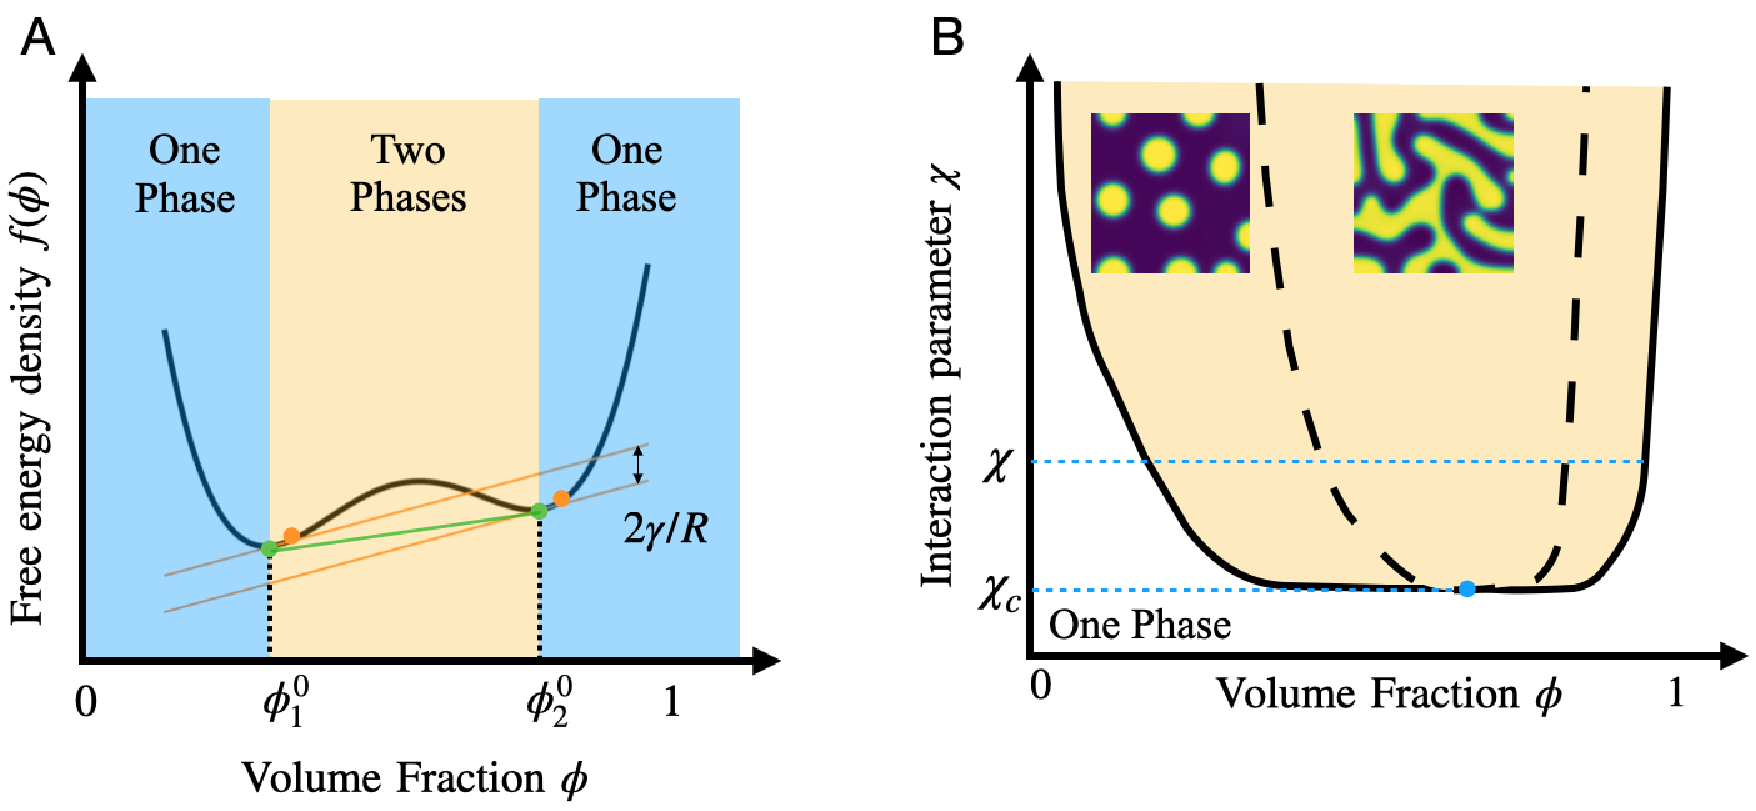
\includegraphics[scale=0.52]{MainContent/Figures/free_energy.pdf}
\caption{\textbf{Schematics of the free energy density for a binary system and the corresponding phase diagram.}
(A) shows schematics for an asymmetric free energy density for $\chi > \chi_c$ as a function of volume fraction $\phi$.
Phase separation is possible only when the average volume fraction lies between $\phi^0_1,~\phi^0_2$.
In the thermodynamic limit, the equilibrium volume fractions $[\phi^0_1,~\phi^0_2]$ (green dots) satisfying \Eqsref{eqn:constraint_1} are the minima of the free energy density.
For the case when phase separation occurs and a droplet of radius $R$ forms, the equilibrium volume fractions (orange dots) shift slightly to the right and the tangents at the equilibrium volume fractions differ in height by a value given by the \textit{Laplace pressure}.
(B) Phase diagram for the system for different interaction parameters $\chi$ as a function of the volume fraction $\phi$.
Below the critical interaction parameter $\chi < \chi_c$, only one phase (the homogeneous state) exists.
The phase boundary (thick black line); also known as the binodal, separates this region from regions where phase separation is possible.  
For $\chi > \chi_c$, lie two different regimes, namely the nucleation and growth regimes and the spinodal decomposition regime.
Between the binodal and the spinodal (dashed black line), we have the nucleation and growth regime which suppresses any infinitesimal perturbations.
For low $\phi$, sufficiently finite perturbations are required for droplets (in yellow) to nucleate and grow in size in the dilute phase (in blue) and for high value of $\phi$, droplets and dilute phase simply swap places.
Note that this regime is possible for low and high values of $\phi$, and for intermediate $\phi$ (spinodal decomposition regime), infinitesimal perturbations grow and system phase separates into bi-continuous structures.
The intersection of the binodal and the spinodal is $\chi_c$ (blue dot), which in the case of equal molecular volumes for $A,~B$ is $\chi_c = 2$ and occurs at $\phi = 0.5$; see Ref. \cite{Review2019}. 
}
\label{fig:free_energy}
\end{figure}

\section{Two-phase co-existence with an interface}

In a system with two phases separated by an interface, the free energy density will have contributions from the interfacial region in terms of the volume fraction $\phi$ and it's spatial gradients $\boldsymbol{\nabla} \phi$; see Refs. \cite{Review2019,Cahn1958}.
After integrating this free energy density with the interfacial contributions over the volume $V$ of the system, the total free energy density of the system reads as a functional of $\phi$; see Refs. \cite{Review2019,Cahn1958}, as:

\begin{equation}
\label{eqn:total_free_energy_FL}
\begin{split}
F[\phi] &= \frac{1}{\nu} \int \mathrm{d}V~ \bigg{[} \frac{\kappa}{2 \nu} |\boldsymbol{\nabla} \phi|^2 + \frac{z}{2} \left[ e_{AA} \phi +  e_{BB} (1 - \phi)\right] \\ & +  k_b T \left[ \phi \ln(\phi) + (1 - \phi) \ln (1 - \phi) + \chi \phi (1 - \phi) \right] \bigg{]}
\end{split}
\end{equation}

However, \Eqref{eqn:total_free_energy_FL} contains logarithmic terms, which can be avoided by considering a simpler form of the total free energy, namely the \textit{Ginzburg-Landau} free energy; see Ref. \cite{Review2019}, which reads as:

\begin{equation}
\label{eqn:total_free_energy_GL}
    F[\phi] = \int \left( f_{\mathrm{GL}}(\phi) +  \frac{\kappa}{2} |\boldsymbol{\nabla} \phi|^2 \right) \mathrm{d}V,
\end{equation}
where $f_{\mathrm{GL}}(\phi)$ is the \textit{Ginzburg-Landau} free energy density and $\kappa > 0$ is a parameter related to the interfacial tension; see Refs. \cite{Zwicker2015,Review2019}.
An important point has to be made from \Eqref{eqn:total_free_energy_GL}: the contribution of the the gradient energy term $\kappa|\boldsymbol{\nabla} \phi|^2 / 2$ gets lower when interface width gets wider or more diffuse; see Ref. \cite{Cahn1958}.
But this reduction in energy can only be compensated by increasing material at the interface, thereby increasing $f_{\mathrm{GL}}(\phi)$.
The gradient term hence penalizes strong variations in the volume fractions across the interface.

The reason we prefer using the \textit{Ginzburg-Landau} free energy density $f_{\mathrm{GL}}(\phi)$ from \Eqref{eqn:total_free_energy_GL} instead of the free energy density given by \Eqref{eqn:flory_huggins} or \Eqref{eqn:free_energy_formulationB} is that $f_{\mathrm{GL}}$ qualitatively captures the relevant features of phase separation such as the existence of two minima, concave and convex regions and a term which represents the interaction term favouring phase separation.
Additionally, the \textit{Ginzburg-Landau} free energy density also has a similar stability criterion and regimes of phase separation; see \figref{fig:free_energy}, as the free energy density given by \Eqref{eqn:flory_huggins} (or \Eqref{eqn:free_energy_formulationB}); see Appendix \ref{sec:phasesep}.

Henceforth, from this point onwards in the thesis, we consider the \textit{Ginzburg-Landau} free energy density which has a simple polynomial form and reads as:
\begin{equation}\label{eqn:free_energy}
    f_{\mathrm{GL}}(\phi) = f(\phi) = \frac{b}{2}(\phi - \phi^{0}_\mathrm{out})^2(\phi - \phi^{0}_\mathrm{in})^2,
\end{equation}
where the minima $\phi^{0}_\mathrm{in}$ and $\phi^{0}_\mathrm{out}$ are the equilibrium concentrations in a thermodynamically large system and $b$ denotes the energy scale.
Typically, we assume that in the thermodynamic limit, $\phi^{0}_\mathrm{in}$ will be a phase rich in droplet material A and $\phi^{0}_\mathrm{out}$ will be a phase rich in dilute phase material B, and hence the notation [in/out].

To summarize, for a system of two phases with an interface, we can calculate the total free energy from \Eqref{eqn:total_free_energy_GL}.
However, we can simply separate the energy contribution of the bulk phases and the energy contribution from the interface; see Ref. \cite{Review2019}, and arrive at explicit relations for the interface width $w$ and surface tension $\gamma$, which we define and discuss in the next section. 

\section{Interface width and surface tension}

In a system of two phases with an interface, we can approximately separate the energy contribution of the bulk phases and the energy contribution from the interface as:
\begin{equation*}
    F \approx V_1 f(\phi_1) + V_2 f(\phi_2) + F_\mathrm{interface},
\end{equation*}
where $F_\mathrm{interface}$ is the free energy associated with the interface.
In a thermodynamically large system, we can assume that if the interface is sharp, i.e. the variation in the phases occurs on a length-scale which is small as compared to the system size, it can be approximated as a surface.
Hence, we can approximate $F_\mathrm{interface} \approx S \gamma$, where $S$ is the surface area of the interface and $\gamma$ is the free energy per surface area of the interface, also known as \textit{surface tension}.

As the gradient term $\kappa|\boldsymbol{\nabla} \phi|^2 / 2$ in \Eqref{eqn:total_free_energy_GL} penalizes strong variations; see Ref. \cite{Cahn1958} in the volume fractions across the phases, it will be the dominant term in \Eqref{eqn:total_free_energy_GL} near the interface.
This forces the system to have a finite interface width $w$, which can be calculated  by considering a flat interface at position $x= 0$ in a one dimensional thermodynamically large system.
The equilibrium volume fractions far from the interface read as $\phi|_{x \rightarrow -\infty} = \phi^0_\mathrm{in}$ and $\phi|_{x \rightarrow \infty} = \phi^0_\mathrm{out}$.
The total free energy of the system given by \Eqref{eqn:total_free_energy_GL} is minimized when the volume fraction profile across the phases reads as:
\begin{equation*}
    \phi(x) = \frac{\phi^0_\mathrm{in} + \phi^0_\mathrm{out}}{2} + \frac{\phi^0_\mathrm{in} - \phi^0_\mathrm{out}}{2} \, \tanh{\left(\frac{x}{w} \right)},
\end{equation*}
where $w$ is the interface width given by $w = 2 \sqrt{\kappa/b}$ in our case; see Refs. \cite{Zwicker2015,Review2019}.

We can also calculate the surface tension $\gamma$ by considering a flat interface of area $S$ at position $x = 0$ in a thermodynamically large system.
The surface tension can now be defined with the contributions from the interfacial region as:
\begin{equation*}
    \gamma = \int_{-\infty}^{+ \infty} \left ( F[\phi(x)] - \frac{F[\phi^0_\mathrm{in}] + F[\phi^0_\mathrm{out}]}{2} \right)~\mathrm{d}x.
\end{equation*}
which in our case reads as $\gamma = (1/6) \sqrt{b/ \kappa}$; see Refs. \cite{Zwicker2015,Review2019}.

Having calculated explicit expressions for surface tension $\gamma$ and interface width $w$, we now assume that we have two phases separated by an interface.
Furthermore, the phase consisting of molecules of $A$ typically forms a droplet of radius $R$ embedded in the phase rich with molecules of $B$ (dilute phase) and we next discuss the effects of surface tension on such finite sized phase separated droplets.

\section{Effect of surface tension on droplets}

Consider a spherical droplet of radius $R \gg w$ formed by liquid-liquid phase separation from the dilute phase in a system of volume $V$. 
Let $\phiEqIn$ and $\phiEqOut$ denote the equilibrium volume fractions of droplet material $A$ inside and outside the droplet respectively.
The total free energy of such a system can simply be approximated by the sum of the contributions from the droplet and the dilute phase as:
\begin{equation}\label{eqn:constraint_3}
    F \approx V_d\,f(\phiIn) + (V - V_d)\,f(\phiOut) + S\,\gamma,
\end{equation}
where $V_d = (4/3) \pi R^3$ is the volume of the droplet, $S = 4 \pi R^2$ is the surface area of the droplet and $\gamma$ is the interfacial surface tension. 
From mass conservation, the total amount of droplet material must be conserved.
Hence,
\begin{equation}\label{eqn:constraint_4}
    V\,\overline{\phi} = V_d\,\phiIn + (V - V_d)\,\phiOut,
\end{equation}
Similar to the treatment for \Eqsref{eqn:constraint_1}, we again minimize the total free energy from \Eqref{eqn:constraint_3} by taking the derivatives with respect to $\phiIn, V_d$ to arrive at the necessary conditions as:

\begin{subequations}
\label{eqn:constraint_5}
\begin{align}
    f'(\phiIn) - f'(\phiOut) &= 0 \mathrm{~and~}
    \\[10pt]
    f(\phiIn) - f(\phiOut) - f'(\phiOut)(\phiIn - \phiOut) + \frac{2 \gamma}{R} &= 0.
\end{align}
\end{subequations}
Similar to \Eqsref{eqn:constraint_1}, the first condition implies that the chemical potential are equal inside and outside the droplet.
Similarly, the second condition states that the difference in the pressure inside and outside the droplet is a term which is directly proportional to a the surface tension $\gamma$ and inversely proportional to the droplet radius $R$, a term also known as \textit{Laplace pressure}; see Ref. \cite{Review2019}.

The equilibrium volume fractions $\phiEqIn,~\phiEqOut$ (orange dots in \figref{fig:free_energy}A) satisfying \Eqsref{eqn:constraint_5} can again be determined from \textit{Maxwell's construction} as follows:
We construct two tangent lines (orange lines in \figref{fig:free_energy}A), which differ in their height by a value of $2 \gamma / R$, and find the points of intersection of these tangents with the free energy density $f(\phi)$.
Note that contrary to the situation of thermodynamic limit, $\phiEqIn,~\phiEqOut$ no longer correspond to the minima of $f(\phi)$, but now get shifted slightly to the right (orange dots in \figref{fig:free_energy}A), as a result of a finite \textit{Laplace pressure}.
In the limit of the droplet radius $R \rightarrow \infty$, we recover $\phiEqIn,~\phiEqOut$ as the minima of $f(\phi)$ (green dots in \figref{fig:free_energy}A). 

We can also explicitly derive the expressions for the equilibrium volume fractions inside and outside the droplet $\phiEqIn,~\phiEqOut$.
From \Eqsref{eqn:constraint_5}, we can expand them as $\phiEqIn = \phi^0_\mathrm{in} + \delta \phiIn$ and $\phiEqOut = \phi^0_\mathrm{out} + \delta \phiOut$ to linear order in $\delta \phiIn$ and $\delta \phiOut$, where $\phi^0_\mathrm{in}$ and $\phi^0_\mathrm{out}$ are the equilibrium volume fractions in the thermodynamic limit; see Ref. \cite{Review2019}.
We then obtain
\begin{subequations}
\label{eqn:delta_phi_in_out}
\begin{align}
    \delta \phiOut &= \frac{2 \gamma}{[\phi^{0}_\mathrm{in} - \phi^{0}_\mathrm{out}] f''(\phi^{0}_\mathrm{out}) R} \mathrm{~and~}
    \\[10pt]
    \delta \phiIn &= \frac{f''(\phi^{0}_\mathrm{out})}{f''(\phi^{0}_\mathrm{in})} \delta \phiOut.
\end{align}
\end{subequations}
Note that $\delta \phiIn,~\delta \phiOut$ are positive, implying that surface tension slightly elevates the equilibrium volume fractions inside and outside the droplets from the basal values $\phi^{0}_\mathrm{in},~\phi^{0}_\mathrm{out}$ (which are the equilibrium volume fractions in the droplet phase and the dilute phase in the thermodynamic limit).
This effect is also inversely proportional to the droplet radius $R$, implying larger droplets are less affected than small droplets. 
This has a consequence when we discuss \textit{Ostwald-Ripening} in detail in a later section. 

To better see the effect of surface tension $\gamma$ on the droplets, we re-write \Eqsref{eqn:delta_phi_in_out} as:
\begin{subequations}
\label{eqn:GibbsThompsonRelations}
\begin{align}
    \phiEq_\mathrm{in} &= \phi^{0}_\mathrm{in} \left (1 + \frac{l_{\gamma, \mathrm{in}}}{R} \right )
    \mathrm{~and~}
    \\[10pt]
    \phiEq_\mathrm{out} &= \phi^{0}_\mathrm{out} \left ( 1 + \frac{l_{\gamma, \mathrm{out}}}{R}\right )
    \;,
\end{align}
\end{subequations}
where $l_{\gamma, \mathrm{out}}$ and $l_{\gamma, \mathrm{in}}$ are capillary lengths given by:

\begin{subequations}
\label{eqn:l_gamma}
\begin{align}
    l_{\gamma, \mathrm{in}} &= (\kappa/b)^{1/2} /[3 \phi^{0}_\mathrm{in} \left(\phi^{0}_\mathrm{in} - \phi^{0}_\mathrm{out}\right)^{3}] \nonumber 
    \mathrm{~and~}
    \\[10pt]
    l_{\gamma, \mathrm{out}} &= (\kappa/b)^{1/2} /[3 \phi^{0}_\mathrm{out} \left(\phi^{0}_\mathrm{in} - \phi^{0}_\mathrm{out}\right)^{3}], \nonumber
\end{align}
\end{subequations}
in the case of the free energy density given by \Eqref{eqn:free_energy} discussed in this thesis.
Since we consider strong phase separation $(\phi^{0}_\mathrm{in} \gg \phi^{0}_\mathrm{out})$, a consequence of \Eqsref{eqn:l_gamma} is $l_{\gamma, \mathrm{out}} \gg l_{\gamma, \mathrm{in}}$, leading to approximating the volume fraction inside the droplet as $\phiIn \approx \phi^{0}_\mathrm{in}$.
Thus, the curvature of the droplets mostly only affects $\phiOut$.
Hence, we finally arrive at the effects of surface tension on the basal values $\phi^{0}_\mathrm{in},~\phi^{0}_\mathrm{out}$, for a droplet of radius $R$.

To summarize, if we start with a homogeneous phase in the spinodal regime (see \figref{fig:free_energy}B), the system is unstable, so any perturbations in the system grow and we end up with two bulk phases; see Appendix \ref{sec:phasesep}. 
However, if we start with a homogeneous phase in the nucleation and growth regime, droplets nucleate for sufficiently high perturbations, and grow by taking up material from the dilute phase.

Having introduced the various phases possible from the free energy density given by \Eqref{eqn:free_energy}, we next introduce the dynamical equations for such phase-separating systems.

% As we are primarily interested in modelling the dynamics of phase separated droplets, in this thesis we will focus solely on the nucleation and growth regime and consider that perturbations are sufficiently finite and droplets form.

\section{Continuous model of phase separation for passive systems}

The dynamics of the system follow from the continuity equation:
\begin{equation*}
    \frac{\partial \phi}{\partial t} + {\boldsymbol{\nabla}} \cdot \vec{j} = 0,
\end{equation*} 
where $\vec{j}$ denotes diffusive fluxes which are driven by gradients in chemical potential $\mu$; see Ref. \cite{Review2019}, which in our case of the free energy density (\Eqref{eqn:free_energy}) becomes:
\begin{equation}
\label{eqn:chemical_potential}
    \mu = \nu \frac{\delta F}{\delta \phi} = b (\phi^{0}_\mathrm{in} - \phi) (\phi^{0}_\mathrm{out} - \phi) (2\phi - \phi^{0}_\mathrm{in} - \phi^{0}_\mathrm{out}) - \kappa \nabla^2 \phi,
\end{equation}
where $\nu$ is the molecular volume of the droplet material.
Linear non-equilibrium thermodynamics implies that the fluxes are proportional to gradients in the chemical potential; see Ref. \cite{Review2019}, which reads as:
\begin{equation*}
    \vec{j} = -\Lambda(\phi) {\boldsymbol{\nabla}}\mu,
\end{equation*}
where $\Lambda(\phi)$ is a positive mobility; see Ref. \cite{GrootBook}.
Hence, the resulting equation takes the form:
\begin{equation} \label{eqn:CHPassive}
    \frac{\partial \phi}{\partial t} = {\boldsymbol{\nabla}} \cdot [\Lambda(\phi) {\boldsymbol{\nabla}} \mu],
\end{equation}
which we will refer to hence-forth in this thesis as the \textit{Continuous model} of phase separation.
\Eqref{eqn:CHPassive} is traditionally also known as the \textit{Cahn-Hilliard} equation; see Refs. \cite{Cahn1958,CahnHilliardEq}, which describes passive phase separation.
In this thesis, we will refer to \Eqref{eqn:CHPassive} and it's counterpart with chemical reactions \Eqref{eqn:CHActive} as the continuous model. 
In particular, two bulk phases with composition $\phi^{0}_\mathrm{in}$ and $\phi^{0}_\mathrm{out}$ typically emerge, which are separated by a typically thin interface of width $w = 2 \sqrt{\kappa/b}$ and surface tension $\gamma = (1/6) \sqrt{b/ \kappa}$.

Consider now a system of droplets formed from sufficiently finite perturbations inside the nucleation and growth regime; see Appendix \ref{sec:phasesep}.
Droplets with smaller radius will have a larger Laplace pressure $(\propto R^{-1})$ and droplets with higher radius will consequently have a smaller Laplace pressure. 
This difference causes a gradient of the chemical potential between the droplets and thus material flows from the smaller to the larger droplets, a process known as \textit{Ostwald-Ripening}; see Ref. \cite{Review2019}.
Eventually, only one droplet remains, and we will elaborate more on this process in Chapter \ref{chap:Chapter_5}.
Naturally, such a coarsening is not favourable for biomolecular condensates, as their size and location needs to be controlled by the cell in order to perform various biomolecular functions.
One such way of suppressing this coarsening behaviour is introduction of chemical reactions and make the system \textit{active}; see Refs. \cite{Zwicker2015,Review2019,Glotzer1995}, which we will discuss in the following section.

\section{Continuous model of passive phase separation with chemical reactions}

We now consider simple chemical reactions which convert the droplet material $A$ into dilute phase material $B$ and vice versa, in which case the individual number of molecules of $A,B$ are no longer conserved, but their sum is.
We assume that the chemical reactions are typically local and can be often described by rate laws that depend on the composition.

In addition, we consider chemical reaction schemes which do not obey detailed balance because in a reaction scheme obeying detailed balance, $A$ and $B$ can convert into each other and the volume fractions $\phiIn, \phiOut$ will relax into states where the total free energy is minimized for a given average volume fraction $\overline{\phi} = \frac{\int_V \phi ~ \mathrm{d}V}{V}$.
This state is usually the homogeneous state consisting of no droplets and hence broken detailed balance is necessary; see Refs. \cite{Zwicker2015,Review2019}.

However, breaking of detailed balance is partly inspired from Biology as well.
For example, $A, B$ can represent two states of a protein with their conversion facilitated by phosphorylation dephosphorylation reactions, when the energy source is adenosine triphosphate molecules; see Ref. \cite{AlbertsBook2003}.
Aguilera-Gomez et al. \cite{Aguilera_Gomez2017} highlighted the general importance of MARylation in the formation and control of condensates in the \textit{Drosophila} oocyte.
Similarly, phosphorylation of NBDY (which is an intrinsically disordered protein) has been shown by Na et al. \cite{Na2021} to be linked with the stability of P-bodies.
Similarly, Saurabh et al. \cite{Saurabh2022} showed in vivo that ATP depletion promotes phase separation in eukaryotic cells, also see Ref. \cite{Pattanayak2020}.

Strong chemical reactions can actually destroy droplets and/or lead to droplet splitting; see Ref. \cite{Zwicker_nature_2016} and they might also lead to more complicated patterns; see Refs. \cite{Glotzer1995,Christensen1996}, which go beyond the scope of this thesis.
Hence, in this thesis, we consider situations in which detailed balance is broken, subsequently leading to novel non-equilibrium effects in the system.
For example, Zwicker et al. \cite{Zwicker2015,Zwicker2014} showed that \textit{Ostwald-Ripening} is shown to be suppressed when simple first order chemical reactions are present between the droplet and the dilute phase material and multiple droplets can co-exist.
Influence of chemical gradients on phase separation has been studied by Weber et al. \cite{Weber2017} and revealed a physical mechanism for arresting droplet ripening.

In this thesis, we focus on situations of weak reaction rates and hence, chemical reactions introduce only a local sink/source term $s(\phi)$ in the continuity equation; see Refs. \cite{Zwicker2015,Review2019}, as:
\begin{equation*}
    \frac{\partial \phi}{\partial t} + {\boldsymbol{\nabla}} \cdot \vec{j} = s(\phi),
\end{equation*}
and the resulting dynamical equation then takes the form:
\begin{equation} \label{eqn:CHActive}
   \frac{\partial \phi}{\partial t} = {\boldsymbol{\nabla}} \cdot [\Lambda(\phi) {\boldsymbol{\nabla}} \mu] + s(\phi).
\end{equation}
and we arrive at the dynamics of the system when local chemical reactions are present.
Note that \Eqref{eqn:CHActive} is a fourth-order, non-linear partial differential equation requiring two boundary conditions for $\phi, ~\mu$.
We here focus on the typical choice of no-flux conditions ($\vec{n} \cdot {\boldsymbol{\nabla}} \mu = 0$) and ($\vec{n} \cdot {\boldsymbol{\nabla}} \phi = 0$), implying that dilute phase and droplet material interact identically with the system's boundaries, whose normal vector is denoted as $\vec{n}$.

\section{Thin interface approximation of the continuous model}

We now arrive at an important junction in this thesis. 
Till now, we have presented basic principles of phase separation for an incompressible binary fluid system and arrived at the effects of chemical reactions on the dynamics of phase separation.

Our aim in this thesis is to numerically simulate phase separation phenomena, in particular, the dynamics of phase separated droplets.
We hence restrict ourselves to the nucleation and growth regimes of phase separation, and do not consider the spinodal growth regime; see \figref{fig:free_energy}B.
Furthermore, we assume that owing to sufficiently finite perturbations, well defined droplets with typical radius $(R \gg w)$ have been phase separated from the dilute phase, and we do not consider any nucleation events.
Simply put, we assume that droplets bigger than the interface width $w$ have been formed as a result of sufficiently finite perturbations in the nucleation and growth regime, whose dynamics we are interested in simulating.

The dynamics of such a system with droplets phase separated from the dilute phase is adequately described by \Eqref{eqn:CHActive}.
But beyond the linear regime (i.e. close to $\phi^0_\mathrm{in}, ~\phi^0_\mathrm{out}$ from \Eqref{eqn:free_energy}), \Eqref{eqn:CHActive} is difficult to solve analytically, as it is non-linear and contains fourth order spatial derivatives.
The continuous model, given by \Eqref{eqn:CHActive}, can also be prohibitively costly to simulate due to multiple reasons:
\begin{enumerate}
    \item The interface needs to be spatially resolved, implying that the spatial discretization of the system should be smaller than the typically small interface width $w$.
    Since we typically consider dilute system of many droplets, simulations are computationally expensive because regions far away from the droplet interfaces typically exhibit very low variation in the volume fraction $\phi$ as seen from Fig. \ref{fig:schematics_CH}.
    
    \item \Eqref{eqn:CHActive} contains fourth order spatial derivatives, which limits the time steps to extremely small values.
    
    \item Interesting and relevant dynamics usually takes place on very long time scales, for instance: during \textit{Ostwald-Ripening}, the length scales in the system evolve as $t^{\,1/3}$ following the Lifshitz-Slyozov-Wagner scaling laws; see Refs. \cite{Lifshitz,Wagner}.
    This typically requires long simulations to capture the relevant behaviour.
\end{enumerate}
Owing to these limitations, simulations of phase separated droplets become extremely computationally expensive.
From typical simulations of phase separated droplets using the continuous model; see Fig. \ref{fig:schematics_CH}, we make certain observations which can enable us to simulate such system of droplets faster and efficiently.

\clearpage

\begin{figure}[tb]
\centering
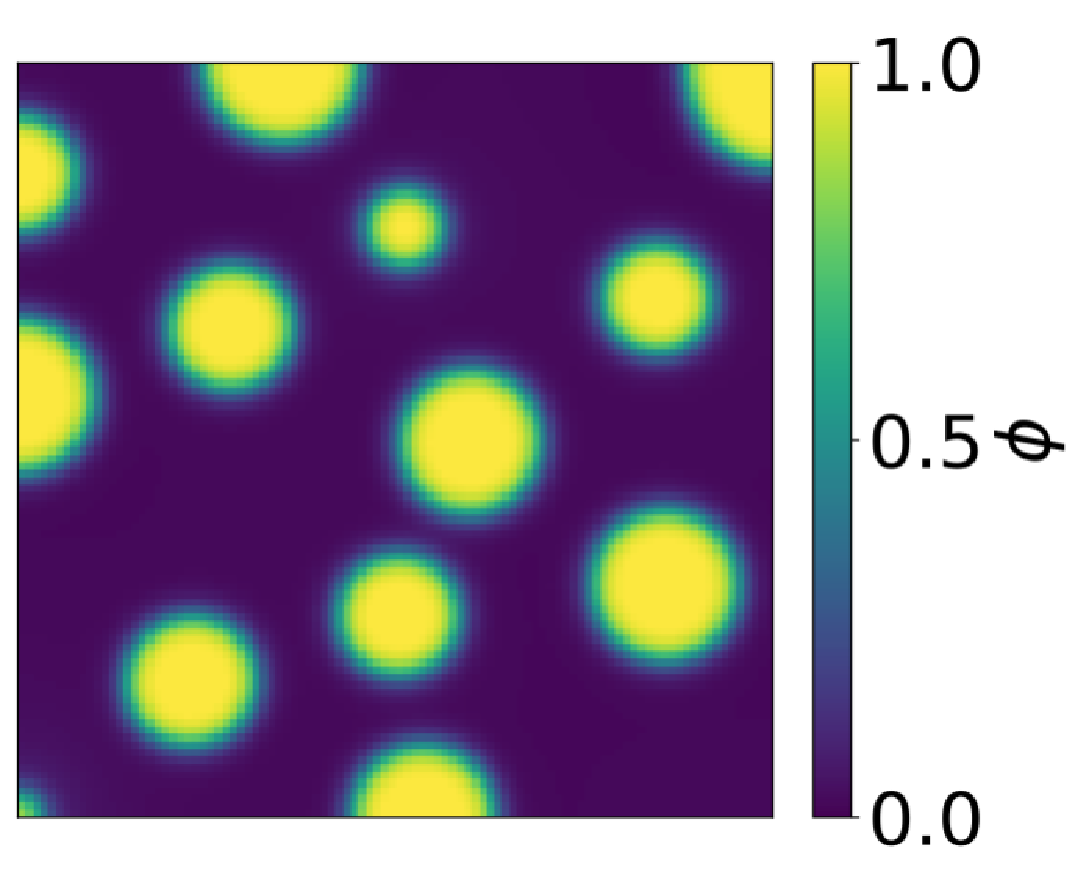
\includegraphics[scale=0.35]{MainContent/Figures/Simulation_CH_Passive.pdf}
\caption{\textbf{Typical simulation state for the continuous model.}
Figure shows a typical state for simulations of the continuous model (\Eqref{eqn:CHActive}, $s(\phi) = 0$) in the nucleation and growth regime depicting the volume fraction field $\phi$.
Phase separated droplets (yellow, with $\phiIn \approx \phi^{(0)}_\mathrm{in}$) are round and variation of $\phiIn,~\phiOut$ in the droplets and dilute phase (blue, with $\phiOut \approx \phi^{(0)}_\mathrm{out}$) itself is low.
The basal values are chosen as $\phi^{(0)}_\mathrm{out} = 0$ and $\phi^{(0)}_\mathrm{in} = 1$ from \Eqref{eqn:free_energy}.
% The continuous model (\Eqref{eqn:CHActive}, $s(\phi) = 0$) uses a two dimensional Cartesian grid of discretization $0.5w$, $w = 2 \sqrt{\kappa / b}$, initial volume fraction $\phi(t=0)$ uniformly chosen from $[\phi = 0.2,0.3]$, $s=0$, $\Lambda = \textcolor{red}{???}$, $\phi^{(0)}_\mathrm{out} = 0$ and $\phi^{(0)}_\mathrm{in} = 1$.
}
\label{fig:schematics_CH}
\end{figure}

The observations we make are:
\begin{enumerate}
    \item Droplets are typically round due to surface tension effects, with the interface $w$ typically smaller than the droplet radius ($R \gg w$).
    Typically, the interfacial width $w$ varies from $10-100\,\mathrm{nm}$; see Ref. \cite{safran_2003}, and is often a small quantity compared to the typical length-scales in the system. 
    
    \item Strong phase separation exists between the droplet and the dilute phases, i.e. $\phi^{0}_\mathrm{in} \gg \phi^{0}_\mathrm{out}$; see \figref{fig:free_energy}A.

    \item Far away from the droplets, spatial variation in the volume fractions is low inside the droplets and the dilute phase itself.

\end{enumerate}
Since we have strong phase separation and low spatial variation of volume fractions inside the droplet phase and inside the dilute phase, we can linearize \Eqref{eqn:CHActive} around $\phi^{0}_\mathrm{in},~\phi^{0}_\mathrm{out}$ to obtain the reaction-diffusion equations which hold inside both the phases; see Ref. \cite{Review2019}, as:

\begin{equation}
\label{eqn:thin_interface_model}
   \frac{\partial \phi_\mathrm{in/out}}{\partial t}
    \approx D_\mathrm{in/out} \nabla^2 \phi_\mathrm{in/out} +
    s(\phi_\mathrm{in/out}),
\end{equation}
where $D_\mathrm{in/out} = \Lambda(\phi^0_\mathrm{in/out})\,b$ is the diffusivity inside the droplets and outside the droplets respectively.
\Eqsref{eqn:thin_interface_model} is known as the \textit{thin-interface approximation}; see Ref. \cite{Zwicker2015}, of the continuous model.

Thus, we arrive at a framework where \Eqsref{eqn:thin_interface_model} enable us to separately consider the volume fractions inside the droplets ($\phiIn$) and outside the droplets, i.e. inside the dilute phase ($\phiOut$).
We will discuss these reaction-diffusion equations for dynamics of droplets and the dilute phase in more detail, in the next chapter.
Note that the quantities $\kappa, w$ and $\Lambda$ act as the link between the continuous model given by \Eqref{eqn:CHActive} and the dynamics of the droplets and dilute phase from \Eqsref{eqn:thin_interface_model}, as $\kappa, w$ appear in \Eqsref{eqn:GibbsThompsonRelations} when evaluating the equilibrium volume fractions for the droplets.

Hence, for phase separated droplets, we have separated the dynamical equations for the droplets and the dilute phase; see \Eqsref{eqn:thin_interface_model}, from the continuous model given by \Eqsref{eqn:CHActive}.
Note that \Eqsref{eqn:thin_interface_model} contain only second order spatial derivatives and hence are potentially much faster to simulate than \Eqsref{eqn:CHActive}.
In the next chapter, we discuss on the procedure of formulating a numerical scheme using \Eqsref{eqn:thin_interface_model} to simulate the dynamics of the droplets and the background field.
Since we separately consider dynamics of the droplets and the dilute phase, the thin interface formulation essentially separates the droplets in the foreground from the dilute phase material in the background. 
Hence, we will call the dilute phase as background field in this thesis from this point on-wards. 

\section{Summary}

In this chapter, we presented the basic principles of Liquid-liquid phase separation for an incompressible binary fluid system using statistical mechanics and linear equilibrium thermodynamics. 
We started with a microscopic picture of phase separation by considering a molecule based lattice model, where we defined interactions between pairs of molecules and used the \textit{mean-field approximation}; see Ref. \cite{Review2019}, to determine the free energy density and internal energy of the system; see \Eqsref{eqn:free_energy_formulation} and the \textit{Flory-Huggins} interaction parameter $\chi$; see \Eqref{eqn:chi}.
We showed from \figref{fig:free_energy}, that for large values of the interaction parameter $\chi > \chi_c$, the free energy density contains both - a concave and a convex part, thus potentially lowering the total free energy and phase separating the homogeneous mixture into two phases. 
Consequently, for $\chi < \chi_c$, only homogeneous phases are possible and thus, no phase separation.

With an aim to arrive at the dynamical equations of phase separation, we first determined the equilibrium volume fractions of the two phases when they phase separated: a) In the thermodynamic limit without an interface, and b) With the inclusion of an interfacial term.
Since we wanted to simulate dynamics of phase separated droplets, we 
focused on the nucleation and growth regimes and assumed finite sized droplets have formed via sufficiently finite perturbations in the homogeneous state.
Taking advantage of the simple form of the \textit{Ginzburg-Landau} free energy density (\Eqref{eqn:free_energy}) over the free energy density given by \Eqref{eqn:flory_huggins}, we used it to derive the effects of interface width $w$ and surface tension $\gamma$ on the equilibrium volume fractions (\Eqsref{eqn:GibbsThompsonRelations}) for droplets and found that they are elevated from the basal values $\phi^0_\mathrm{in},~\phi^0_\mathrm{out}$; see \Eqref{eqn:free_energy}.

We then derived the dynamical equations for passive phase separation by considering that gradients in chemical potential $\mu$ drive the material fluxes and arrived at the traditional \textit{Cahn-Hilliard} equation describing passive phase separation, given by \Eqref{eqn:CHPassive}. 
Next, we took into account the effect of local and weak chemical reactions, which break detailed balance and lead to novel physics, on passive phase separation and arrived at the dynamical equation for the system in presence of chemical reactions given by \Eqref{eqn:CHActive}.

Finally, we showed the limitations and drawbacks in simulating the continuous model; given by \Eqref{eqn:CHActive}, for simulating the dynamics of phase separate droplets.
Based on valid assumptions, we then formulated an approximated analytical model; given by \Eqsref{eqn:thin_interface_model}, which described the separation of the dynamics of droplets and the dilute phase using simple reaction-diffusion equations.
\clearpage

% Chapter 3

\onehalfspacing

\chapter{Effective simulations of droplets}

\label{chap:Chapter_3}

In the previous chapter, we developed the framework for separately describing the volume fraction inside the droplets ($\phiIn$) and outside the droplet i.e. inside the background field ($\phiOut$).
From typical simulations of the continuous model given by \Eqref{eqn:CHActive}; see \figref{fig:schematics_CH}, we assumed that:
\begin{enumerate}
    \item Strong phase separation exists between the droplet material and the background field, i.e. $\phi^0_\mathrm{in} \gg \phi^0_\mathrm{out}$.

    \item $\phiIn,~\phiOut$ themselves vary little inside the droplet and the background field respectively and can be modelled using simple reaction-diffusion equations.
\end{enumerate}
We thus arrived at the thin-interface approximation; see \Eqsref{eqn:thin_interface_model} of the continuous model.
We next focus on utilizing this framework to develop a numerical model to simulate dynamics of phase separated droplets and background field, known henceforth as the effective droplet model.

The aim of the effective droplet model is to replace the detailed description of the entire volume fraction field; given by \Eqref{eqn:CHActive}, by the relevant degrees of freedom of the droplets.
In a typical situation of well-separated droplets that are spherical due to surface tension, droplets are adequately described by their position $\vec{x}_i$, radii $R_i$ and volume fraction $\phiIn$.
The background field $\phiOut$ and the droplets are naturally coupled through material exchanges, which we discuss and model in the subsequent sections.
Since material fluxes across the interface of the droplets give rise to their growth and drift, we start by formulating dynamical equations for volume fractions $\phiIn,~\phiOut$, evaluating determining material fluxes, thus systematically building up the effective droplet model. 

\section{Volume fraction and fluxes inside droplets}

We begin by considering a single droplet of radius $R \gg w$ embedded in a large background field.
Since $\phi_\mathrm{in}$ typically varies only a little inside the droplets and remains close to $\phi^{0}_\mathrm{in}$, we linearize $\phi_\mathrm{in}$ around $\phi^{0}_\mathrm{in}$ to obtain the dynamical equation from the thin-interface approximation; see \Eqsref{eqn:thin_interface_model}, as:
\begin{align} 
    \label{eqn:RD_droplet}
    \frac{\partial \phi_\mathrm{in}}{\partial t}
        \approx D_\mathrm{in} \nabla ^2 \phi_\mathrm{in} +
        s(\phiIn),
\end{align}
where $D_\mathrm{in} \approx \Lambda(\phi^0_\mathrm{in})\,b$ is the diffusivity inside the interface of the droplet.
Since $\phi_\mathrm{in}$ is linearized around $\phi^{0}_\mathrm{in}$, the reaction flux $s(\phi_\mathrm{in})$ inside the droplet can also be linearized around $\phi^{0}_\mathrm{in}$ as:
\begin{equation*}
    s(\phi_\mathrm{in}) \approx s(\phi^{0}_\mathrm{in}) - k_{\mathrm{in}}(\phi_\mathrm{in} - \phi^{0}_\mathrm{in}),
\end{equation*}
where $k_{\mathrm{in}}= - s'(\phi^{0}_\mathrm{in})$ denotes the reaction rate; see Ref. \cite{Review2019}.
Note that positive rates ($k_\mathrm{in}>0$) stabilize the fraction $\phi_\mathrm{in}$, while large negative rates might destabilize leading to unstable droplets.
% However, this instability is suppressed when we consider weak chemical reactions.
% Low reaction rates increase the value of the reaction-diffusion lengthscale $\xi_\mathrm{in}=\sqrt{D_\mathrm{in}/|k_{\mathrm{in}}|}$. 
% The droplet radius $R$ is then small compared to the $\xi_\mathrm{in}$; see Ref. \cite{Review2019}, and our assumption for ($R \ll \xi_\mathrm{in}$) is valid.
However, the instability is suppressed when the droplet radius $R$ is small compared to the reaction-diffusion length-scale, $\xi_\mathrm{in}=\sqrt{D_\mathrm{in}/|k_{\mathrm{in}}|}$; see Ref. \cite{Review2019}.
Since we here consider weak chemical reactions, $\xi_\mathrm{in}$ will be large, and we thus assume that $R \ll \xi_\mathrm{in}$ holds.

We then solve \Eqref{eqn:RD_droplet} in stationary state in a spherically symmetric system with boundary conditions $\phi_\mathrm{in}(R) = \phiEq_\mathrm{in}$ and $\partial_r  \phi_\mathrm{in}(0) = 0$; 
% The linearization works particularly well when the droplet radius $R$ is small compared to the reaction-diffusion length-scale namely, $\xi_\mathrm{in}=\sqrt{D_\mathrm{in}/|k_{\mathrm{in}}|}$.
The analytical result for $\phi_\mathrm{in}$ allows us to estimate the diffusive flux $\vec{j}_\mathrm{in}$ inside the droplet; see Appendix \ref{sec:fluxes_inside_droplets}, as:
\begin{equation}
	\label{eqn:flux_inside}
    \vec{j}_\mathrm{in}  \approx [-D_\mathrm{in} {\boldsymbol{\nabla}} \phi_\mathrm{in}(R)]\,\vec{n} \approx \frac{R}{d}~ s(\phiEqIn)~\vec{n}
    \;,
\end{equation}
where $d$ is the space dimension and the normal vector to the droplet surface is denoted by $\vec{n}$.
Note that production of droplet material inside the droplet ($s(\phiEqIn) > 0$) leads to an outward flux $\vec{j}_\mathrm{in} \cdot \vec{n} > 0$, which can drive droplet growth.
Conversely, destroying droplet material ($s(\phiEqIn) < 0$) drives shrinking droplets.
Having estimated the fluxes inside the droplet, we next discuss dynamics of $\phiOut$ in the background field. 

\section{Dynamics of the background field}

Droplets might also grow if they take up material from the surrounding.
Spatial gradients of $\phiOut$ outside the droplet surface lead to material fluxes into the droplet.
In general, $\phiOut$ can be calculated by considering that it will typically vary only little and stay close to $\phi^0_\mathrm{out}$.
Similarly as inside the droplets, we can then linearize around the base value $\phi^0_\mathrm{out}$ to obtain the reaction-diffusion equation from the thin-interface approximation; see \Eqsref{eqn:thin_interface_model}, as:
\begin{equation} 
	\label{eqn:RD_dilute}
	\frac{\partial \phiOut}{\partial t} \approx 
	    D_\mathrm{out} \nabla ^2 \phiOut + s(\phiOut),
\end{equation}
where $D_\mathrm{out} = \Lambda(\phi^0_\mathrm{out})~b$ is the diffusivity outside the droplets.
Thus, in principle, both $\phiIn,~\phiOut$ can be analytically calculated from \Eqref{eqn:RD_dilute} and \Eqref{eqn:RD_droplet} with appropriate boundary conditions.

\section{Interfacial velocity and dynamics of the droplets}

Material fluxes across droplets are responsible for their growth and drift; see Refs. \cite{Review2019,Weber2017}.
If we know the volume fraction profiles $\phiIn,~\phiOut$ from \Eqref{eqn:RD_droplet} and \Eqref{eqn:RD_dilute}, we can then evaluate the fluxes $\jIn$ (inside the droplet) and $\jOut$ (outside the droplet) to determine the net accumulation of droplet material at the interface, which implies droplet growth.
Note that only the normal components of the fluxes affect the shape, while the tangential components merely re-distribute material parallel to the interface.
In general, these shape changes of the isolated droplet are described by the interfacial speed as $\partial_t R = \vn /  (\vec{e_r} \cdot \vec{n})$; see Refs. \cite{Review2019,Weber2017,Seyboldt_2018}, where $\vec{e_r}$ is the position unit vector to the droplet surface.
Since surface tension effects typically ensure a near-spherical shape, the interfacial speed $\vn$ (see Appendix \ref{sec:interfacial_speed_derivation}) for spherical droplets can be written as:
% derived as follows.
% Consider an isolated droplet of radius $R$ and position $\vec{x}$. The amount of material in the droplet is given by $\Phi = \phiEqIn\,V$, where $V$ is the volume of the droplet.
% The rate of change of $\Phi$ then looks like:
% \begin{equation}
%     \partial_t {\Phi} \approx [\partial_t {V}]\,\phiEqIn + [\partial_t {\phiEqIn}]\,V,
%     \label{eqn:volume_change1}
% \end{equation}
% where we assume weak chemical reactions.
% Additionally, we also have $\partial_t {\Phi} \approx S \, (\jIn - \jOut) \cdot \vec{n}$, where $S$ is the surface area of the droplet.
% Consequently $\partial_t {V} = S\,\partial_t {R} = S\,v_\mathrm{n}$.
% Hence it follows from \Eqref{eqn:volume_change1}:
% \begin{equation}
%     S\,(\jIn - \jOut) \cdot \vec{n} \approx S\,v_\mathrm{n}\,\phiEqIn + V~\partial_t{\phiEqIn}.
%     \label{eqn:volume_change2}
% \end{equation}
% As $\phiEqIn$ depends on the droplet radius $R$ as well, we use the chain rule to obtain $\partial_t{\phiEqIn} = \partial_R{\phiEqIn} \times \partial_t{R} = v_\mathrm{n} \, \partial_R{\phiEqIn}$, after using $\partial_t R = \vn / (\vec{e_r} \cdot \vec{n}) = \vn$, as $\vec{e_r} \cdot \vec{n} = 1$ for spherical droplets. 

% Finally, substituting the expressions for $\partial_t{\phiEqIn},~\phiEqIn$ in \Eqref{eqn:volume_change2} gives us the dynamical equation for the interfacial speed as:
\begin{equation}
    \label{eqn:InterfacialSpeed}
    \vn \approx \frac{\jIn - \jOut}{\phiEqIn - \phiEqOut} \cdot \vec{n}.
\end{equation}
We thus have an expression for droplet growth in terms of the fluxes $\jIn,~\jOut$.
Generally, these fluxes can result in shape fluctuations and non-spherical droplets; see Refs. \cite{Review2019,Zwicker_nature_2016}.
As we consider spherical droplets, it enables us to finally describe the dynamics of spherical droplets; see Appendix \ref{sec:droplet_dynamics}, as:
\begin{subequations}
\label{eqn:droplet_dynamics}
\begin{align}
	\label{eqn:DropletGrowth}
	\frac{\mathrm{d}R}{\mathrm{d}t} & = \frac{1}{S} \int_{\Omega} \vn \,\mathrm{d}A
	\qquad \text{and}
    \\[10pt]
	\label{eqn:DropletDrift}
	\frac{\mathrm{d} \vec{x}}{\mathrm{d}t} &= \frac{d}{S} \int_{\Omega} \vn \vec{n}\,\mathrm{d}A,
\end{align}
\end{subequations}
where the integral is over the droplet surface $\Omega$, $d$ is the space dimension and $S$ is the surface area of the droplet. 
Thus, we arrive at a framework, where we can determine the growth and drift of a single isolated droplet if we know the fluxes $\jIn,~\jOut$ inside and outside the droplet interface.

To summarize, \Eqsref{eqn:droplet_dynamics} determine how an isolated droplet evolves in time.
This involves calculating $\phiEqIn,~\phiEqOut$ from \Eqsref{eqn:GibbsThompsonRelations}, $\jIn$ from \Eqref{eqn:flux_inside}, the interfacial speed $v_\mathrm{n}$ from \Eqref{eqn:InterfacialSpeed} and most importantly, the fluxes $\jOut$ outside the droplet interface.
Evaluating $\jOut$ is a central part of our model, which we discuss next.

%%%%Section separator %%%%

\section{Numerical model for many spherical droplets}

We next present the methodology to derive the flux $\jOut$ outside each droplet and derive the numerical counterpart for \Eqsref{eqn:droplet_dynamics} in order to arrive at the discretized dynamics of the droplets. 
We first consider the dynamics of the volume fraction of the background field $\phiOut$.
In principle, the dynamics of $\phiOut$ follows from \Eqref{eqn:RD_dilute}, with appropriate boundary conditions applied at the system's boundary and at all droplet surfaces.
However, that would mean solving for $\phiOut$ on the entire domain with \textit{holes} at the locations of the droplets, which would be numerically expensive and would potentially involve knowing spatially resolved background field near the droplets.

However, we can simplify the description of the background field as variation in $\phiOut$ is low and hence $\phiOut$ typically stays close to $\phi^0_\mathrm{out}$.
% We can hence assume that $\phiOut$ is defined in the entire system - including where droplets are present, as the numerical value for $\phi^0_\mathrm{out}$ in our choice of free energy density is low.
We can hence assume that $\phiOut$ spans the entire domain, including where droplets are present, as the numerical value for $\phiOut$ is small.
This is a crucial assumption in our model, as this removes the computationally expensive part to solve for the dynamics of $\phiOut$ on a complicated domain.

Hence in this description, we completely `de-couple' droplets from the background field and consider the droplets as local perturbations to background field at their respective locations; see \figref{fig:schematics}A.
We next briefly discuss the dynamics of the background field $\phiOut$ and return to dynamics of $\phiIn$ inside the droplets later.

\begin{figure}[tb]
\centering
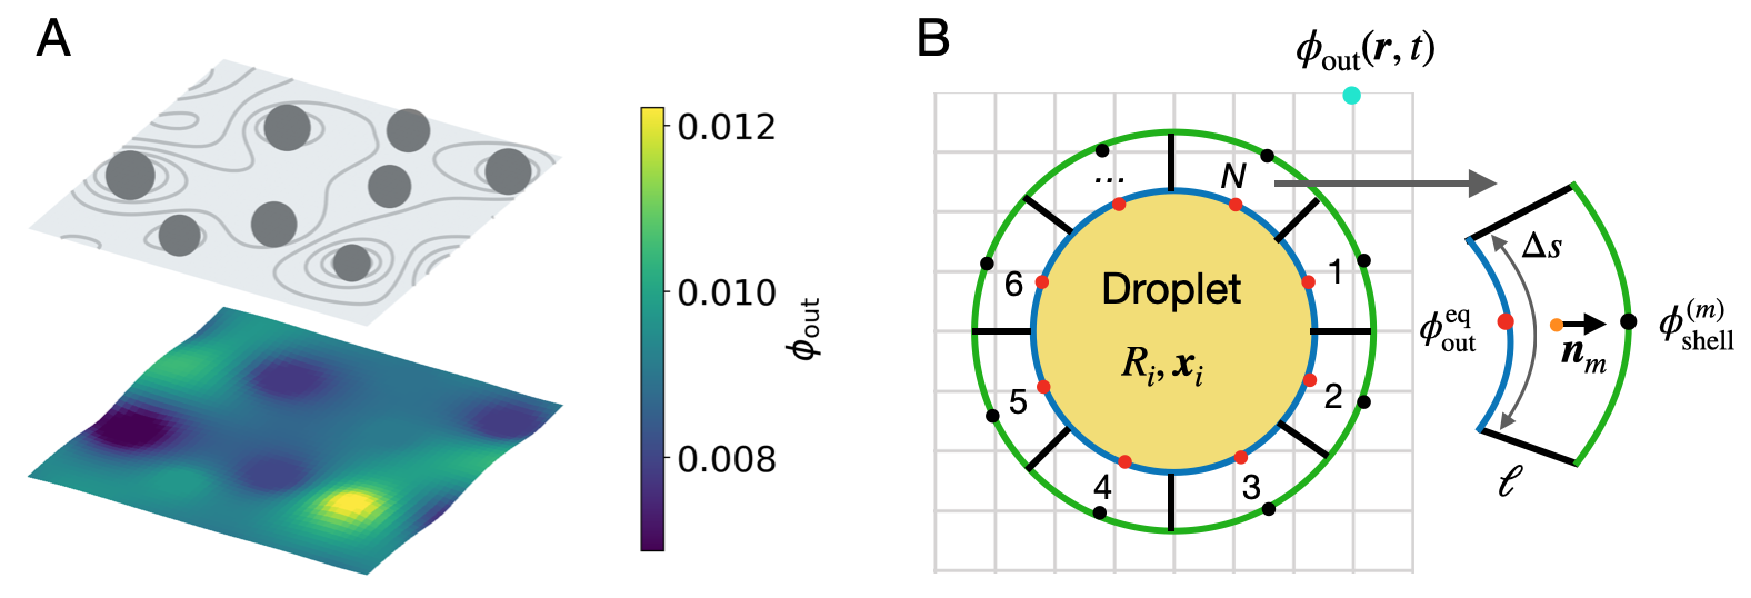
\includegraphics[scale=0.53]{MainContent/Figures/simulation.pdf}
\caption{\textbf{Schematics of the simulation model, describing droplets and the background field $\phiOut$.}
(A) Droplets (top plane, gray spheres) co-exist with the background field $\phiOut$ (bottom plane) and interact with it only through material fluxes.
For simplicity, $\phiOut$ also exists at the location of the droplets, but this has negligible effect on the dynamics.
Gray lines (top plane) show lines of similar background field $\phiOut$.
Dense lines indicate higher $\phiEqOut$ for smaller droplets.
(B) Isolated droplet (yellow) with a surrounding shell of thickness $\ell$ (green), which is further discretized in $N$ sectors of linear size $\ds$.
The exchanged fluxes between droplet and background are determined in each sector based on the equilibrium fraction $\phiEqOut$ (red dots) and the value $\phiOut^{(m)}$ at the outer side (black dot), which is determined from the background field using linear interpolation.
The background field $\phiOut$ is uniformly discretized on a Cartesian grid (cyan dots, gray grid).
}
\label{fig:schematics}
\end{figure}


\subsection{Dynamics of the background field}

Generally, the dynamics of the background field $\phiOut$ is affected due to diffusion and reactions, even if droplets are absent.
Additionally, if the droplets are present, material fluxes might flow in or out of the background field, eventually affecting the dynamics of $\phiOut$.
To numerically capture the dynamics of $\phiOut$, we discretize the continuous field $\phiOut$ on a uniform Cartesian grid with a spatial discretization $\dx$ between the neighbouring support points.
We then evolve \Eqref{eqn:RD_dilute} for a given chemical reaction scheme $s(\phiOut)$ in time using finite differences and an explicit temporal stepping, using a simulation package \textit{py-pde}, written in \textit{Python} and developed in the Zwicker Group; see Ref. \cite{Zwicker2020}.

Note that since we do not need to resolve droplets at this scale, the spatial discretization $\dx$ can be much larger than the interface width $w$, enabling us to simulate the background field using \Eqref{eqn:RD_dilute} at significantly lower computational costs (and higher speeds) compared to the continuous model \Eqref{eqn:CHActive}.
We next discuss the extent to which a single droplet alters $\phiOut$ in it's vicinity, enabling us to approximately calculate $\jOut$ outside the droplet. 

\subsection{Single droplet in an anisotropic environment}

To obtain the fluxes in the outer vicinity of an isolated droplet, we need to determine $\phiOut$ in the region surrounding this droplet.
In general the vicinity of the droplet might be anisotropic.
We discretize the heterogeneous vicinity of the droplet by constructing an annular region of thickness $\ell$ surrounding the droplet.
We further discretize this shell into $N$ annular shell sectors; see Fig. \ref{fig:schematics}B, to resolve spatial anisotropies of $\phiOut$ near the droplet.
These sectors are chosen uniformly in the angular directions for 2 and 3 dimensions and we assume that $N$ is large so that fluxes in the angular directions are negligible.

We then denote the volume fraction of the droplet material in the $m$-th sector as $\phiOut^{(m)}(r)$, where $r$ is a radial coordinate measuring the distance of the droplet surface from the droplet position $\vec{x}$.
Assuming that the dynamics of $\phiOut^{(m)}(r)$ in the shell sector relaxes quickly relative to the droplet growth and drift, we can determine $\phiOut^{(m)}(r)$ using \Eqref{eqn:RD_dilute} in stationary state along with the boundary conditions $\phiOut^{(m)}(R)=\phiEqOut$ and $\phiOut^{(m)}(R + \ell)= \phiShell^{(m)}$.
Here, $\phiShell^{(m)}$ is the fraction of droplet material in the background field at the outer side of the $m$-th shell sector, which we estimate from a linear interpolation of the discretized background field $\phiOut$; see Fig. \ref{fig:schematics}B.
Thus $\phiShell^{(m)}$ is an approximate representative volume fraction of the background field at the outer surface of the shell. 
Solving \Eqref{eqn:RD_dilute} would require information about the reaction flux $s(\phiOut)$ inside the shell sector, which we will discuss next.

Next, we focus our attention on the reaction flux inside the sector, given by $s(\phiOut^{(m)})$ from \Eqref{eqn:RD_dilute}, and determine it's effect on the dynamics of $\phiOut^{(m)}(r)$ inside the $m$-th shell sector.
We assume that $\phiOut^{(m)}(r)$ varies only marginally in the shell sector which allows us to linearize the reaction flux as a function of $\phiOut^{(m)}$ as:
\begin{equation*}
    s(\phiOut^{(m)}) \approx \Gamma_\mathrm{out} - \kOut~\phiOut^{(m)},
\end{equation*}
where
\begin{subequations} 
\label{eqn:GammaOut_KOut}
\begin{align}
    \Gamma_\mathrm{out} &= \frac{\phiShell^{(m)}~s(\phiEqOut) - \phiEqOut~s(\phiShell^{(m)})}{\phiShell^{(m)} - \phiEqOut} 
    \qquad \text{and}
    \\[10pt]
    \kOut &= \frac{s(\phiEqOut) - s(\phiShell^{(m)})}{ \phiShell^{(m)} - \phiEqOut},
\end{align}
\end{subequations}
are obtained from the boundary constraints $s(\phiOut^{(m)})(R) = s(\phiEqOut)$ and $s(\phiOut^{(m)})(R + \ell) = s(\phiShell^{(m)})$.
Taken together, the dynamics of $\phiOut^{(m)}(r)$ inside the shell sector can finally be determined from the steady state of \Eqref{eqn:RD_dilute} as:

\begin{equation}
\label{eqn:phi_out_in_shell}
     D_\mathrm{out}  \nabla ^2 \phiOut^{(m)}(r) + \Gamma_\mathrm{out} - \kOut~\phiOut^{(m)}(r) \approx 0,
\end{equation}
which can be analytically solved for $\phiOut^{(m)}(r)$; see Appendix \ref{sec:fluxes_inside_shell}.
Note that here we implicitly assume that the angular discretization of the shell is small enough, so that $\phiOut^{(m)}$ is only a function of the radial co-ordinate, which is the case for a large $N$.

Solving for $\phiOut^{(m)}$ gives us the local material fluxes outside the droplet surface for each sector in the normal direction as $\jOut^{(m)} \cdot \vec{n} = [-D_\mathrm{out} {\boldsymbol{\nabla}} \phiOut^{(m)}(R)] \cdot \vec{n} $, where $D_\mathrm{out}$ is the diffusivity outside the droplet.
We thus arrive at the fluxes outside the droplet; see Appendix \ref{sec:fluxes_inside_shell}.
Knowing the flux $\jOut^{(m)} \cdot \vec{n}$ outside each droplet for each $m$-th shell sector, we next determine the growth and drift of a system of droplets.

\subsection{Growth and drift of a system of droplets}

To briefly summarize, we obtain an analytical approximation of $\phiOut^{(m)}(r)$ in each shell sector, from which we determine the local flux $\jOut^{(m)}$ for a shell sector of a single isolated droplet.
We now consider a system of droplets much bigger than the interface width ($R \gg w)$ and neglecting the small value of $\phiEqOut$, the interfacial velocity then reads from \Eqref{eqn:InterfacialSpeed} as:
\begin{equation*}
    % \label{eqn:InterfacialSpeed_simplified}
    v_\mathrm{n} \approx \frac{\jIn - \jOut}{\phiEqIn} \cdot \vec{n},
\end{equation*}
Using the expression for $\jIn$ from \Eqref{eqn:flux_inside} along with the expression for $\jOut^{(m)} \cdot \vec{n}$ for the $m$-th shell sector; see Appendix \ref{sec:fluxes_inside_shell}, we finally arrive at a discretized form of \Eqsref{eqn:droplet_dynamics} for each droplet as:

\begin{subequations} 
\label{eqn:DropletDiscretized}
\begin{align}
    \frac{\Delta R}{\Delta t} &\approx \frac{1}{\phiEqIn}~\sum_{m=1}^{N} \frac{A_m}{S}\left ( \frac{R}{d}~s(\phi^\mathrm{eq}_\mathrm{in})  -  {j}^{(m)}_\mathrm{out}  \right)
    \mathrm{~and~}
    \\[10pt]
    \frac{\Delta \vec{x}}{\Delta t} &\approx \frac{d}{\phiEqIn}~\sum_{m=1}^{N} \frac{A_m}{S} \left ( \frac{R}{d}s(\phi^\mathrm{eq}_\mathrm{in})  -  {j}^{(m)}_\mathrm{out}\right) \vec{n}_m,
\end{align}
\end{subequations}
where $R, S, V$ are the radius, surface area and volume of the droplet respectively, $d$ is the space dimension, $A_m$ is the inner area of the shell sector, $d$ is the space dimension and $\vec{n}_m$ is the unit vector pointing from the droplet center to the $m$-th shell center; (orange dot, see \figref{fig:schematics}B).
\Eqsref{eqn:DropletDiscretized} can then be easily extended to encompass the description of multiple droplets and we thus arrive at the set of dynamical equations for describing growth and drift of a system of droplets.
Note that for the droplets to drift, the fluxes $\jOut^{(m)}$ necessarily need to be anisotropic with respect to the droplet.
This can be easily seen from the fact that if the droplet vicinity is isotropic, the droplet will simply grow and not drift. 

We thus use \Eqsref{eqn:DropletDiscretized} to describe how internal reactions and external material exchange with the background field affects the dynamics of each droplet.

\subsection{Coupling of droplets and background field}

We next describe a crucial part of the numerical scheme which involves coupling of the droplets with the background field. 
\Eqsref{eqn:DropletDiscretized} describes how droplets change when they take up droplet material from the background field $\phiOut$.
Recall that the local flux $\jOut^{(m)} \cdot \vec{n}$ enters the shell sector at the inner shell sector boundary (red points in \figref{fig:schematics}B).
Due to material conservation, the integrated flux $\Sigma = \jOut^{(m)} \cdot \vec{n}\,A_m$ needs to be removed from the background field $\phiOut$ for each shell sector of each droplet at the midpoint of the inner shell sector boundary (red points in \figref{fig:schematics}B).
Similar to the procedure when estimating $\phiShell^{(m)}$ from $\phiOut$, we again use a linear interpolation to remove the respective amount from the background field $\phiOut$.
Note that negative fluxes $\jOut^{(m)}$ distribute material from the droplets to the background field.
This procedure ensures that the total material flux toward the droplet is taken from the background field and it preserves potential anisotropies of the exchange.

\subsection{Choosing the time-step $\dt$}

We discuss the procedure for calculating the time-step $\dt$ used in the numerical model, which is a crucial simulation parameter as it potentially affects droplet growth and drift; see \Eqsref{eqn:DropletDiscretized}, as well as the dynamics of the background field $\phiOut$; see \Eqref{eqn:RD_dilute}.
Naturally, we wish to select a maximum allowed time-step which accurately captures the dynamics of the droplets and the background field. 

Hence, $\dt$ should be chosen based on the minimum of the time-steps involved when evolving:
\begin{enumerate}
    \item The dilute field $\phi_{\mathrm{out}}$ in time, according to \Eqref{eqn:RD_dilute}.
    
    \item The dynamics of the background $\phiShell^{(m)}(r)$ inside the $m$-th shell sector, as described by \Eqref{eqn:phi_out_in_shell}.
    
    \item The dynamics of the droplets in time, according to \Eqsref{eqn:DropletDiscretized}.
    
    \item The time-step arising from chemical reactions.
\end{enumerate}
Naturally, smaller values of $\dt$ imply more accurate simulations and larger values result in faster (but less accurate) simulations.
% ; although very low or very high time-steps numerical instabilities might also render the simulations unstable.
% These instabilities can potentially arise from choosing a small shell thickness $\ell$, which results in a large value of fluxes outside the droplet $\jOut^{(m)} \cdot \vec{n}$, as they scale with $\ell^{-1}$; see Appendix \ref{sec:fluxes_inside_shell}.
% Another potential area of origin for instabilities is when $\ds$ is a small quantity, which 
We next separately analyze the dynamics of the background field, the shell, and the droplet growth to identify the maximal suitable value of $\dt$.

In general, the time-step for evolving \Eqref{eqn:RD_dilute} is determined from the mutual interplay between reactions and diffusion.
A standard von Neumann stability analysis of \Eqref{eqn:RD_dilute} shows that our numerical scheme is stable if $\dt < \dx^2/(2 D_\mathrm{out})$, where $D_\mathrm{out}$ is the diffusivity outside the droplet.
Consequently, a suitable time-step for evolving the background field is $\dt_\mathrm{background} = 0.1 \dx^2/D_\mathrm{out}$, where we choose the constant pre-factor conservatively as $0.1$ instead of $0.5$.
Similarly, we define $\dt_\mathrm{shell} = 0.1 \ell^2/D_\mathrm{out}$ for the shell.
We also consider the time scale of reactions, $\dt_\mathrm{reaction} = 0.1 / (\max_\phi |s(\phi)|)$, based on the maximal rate of $s(\phiOut)$ to accurately capture the effect of chemical reactions on the dynamics of $\phiOut$.

Finally, to ensure that the dynamics of droplet growth is captured correctly, we assume the droplet growth rate ($\Delta R / \Delta t$) at each time-step to be proportional to their radius $R$ (neglecting the $1/R^2$ dependence); see Ref. \cite{Review2019}, and limit the droplet growth rate from \Eqsref{eqn:DropletDiscretized} to $10\%$ of their previous size.
In other words, we place a restriction such that the relative growth of a single droplet $R^{-1}\abs{\diff R/\diff t}$ is small during a single time-step $\dt$.
Assuming that typical droplets are not much smaller than the mean initial droplet radius~$\mean{R}$, this implies a maximal time-step $\dt_\mathrm{droplets} = 0.1 \mean{R}^2/D_\mathrm{out}$.
This is specially important when considering mean-field simulations as time-step $\dt$ would be too high if it is calculated solely on the basis of the shell thickness $(\dt_\mathrm{shell})$ and the background field discretization $(\dt_\mathrm{background})$.
Such a large time-step will erroneously calculate the droplet dynamics from \Eqsref{eqn:DropletDiscretized} and hence we have to consider the size of the droplets as well when calculating the time-step $\dt$.
Finally, we choose the time-step $\dt$ which is a conservative minimum of all the different time-steps mentioned above, i.e.
\begin{equation}
\label{eqn:time_step}
    \dt = 0.1 \, \mathrm{min \, }\left[  \frac{0.1 \dx^2}{D_\mathrm{out}}, \frac{0.1 \mean{R}^2}{D_\mathrm{out}}, \frac{0.1 \ell^2}{D_\mathrm{out}}, \frac{0.1}{(\max_\phi |s(\phi)|)} \right ].
\end{equation}

\subsection{Algorithm and full simulation}

The full numerical method involves evolving the state of the system, i.e., the discretized background field $\phiOut(\vec{r})$ and the positions $\vec{x}_i$ and radii $R_i$ of all droplets in time.
We perform an explicit iteration in time, where the state at $t + \dt$ is directly determined from the state at time $t$.
We first evolve the reaction-diffusion equation \Eqref{eqn:RD_dilute} of the background field and then iterate over all droplets.
For each droplet, we determine the fluxes $\jOut^{(m)} \cdot \vec{n}$ outside the $m$-th sector. We then remove the associated material from the background field for all $N$ shell sectors and update the droplet's position and radius according to \Eqsref{eqn:DropletDiscretized}.
Starting from an initial state at $t=0$, the numerical algorithm (see Algorithm \ref{alg:algorithm}), allows us to evolve the dynamics forward in time.

\section{Summary}

As we were interested primarily in simulating dynamics of phase separated droplets and background field, we built upon the thin-interface approximation model given by \Eqsref{eqn:thin_interface_model} from Chapter \ref{chap:Chapter_2}, which separately describes the dynamics of droplets and the background field.
This model is an approximation of the continuous model given by \Eqref{eqn:CHActive}.
To accurately model the dynamics of the droplets, we needed to calculate the material fluxes in the droplets $\jIn$ and outside the droplets $\jOut$, which govern how much material enters or exits the droplets, thus affecting their dynamics.

We first described the dynamical equations for the volume fraction inside the droplet $\phiIn$ from \Eqref{eqn:RD_droplet} and calculated $\jIn$ from \Eqref{eqn:flux_inside} based on chemical weak reactions.
Assuming that we knew the volume fraction outside the droplets $\phiOut$ in principle from \Eqref{eqn:RD_dilute}, $\jOut$ outside the droplet could then be evaluated, leading to the interfacial speed $\vn$ from \Eqref{eqn:InterfacialSpeed}, which led us to formulating the dynamical equations of growth and drift for spherical droplets given by \Eqsref{eqn:droplet_dynamics}.

We then focused on calculating the fluxes outside the droplets $\jOut$, which stem from spatial gradients in $\phiOut$.
In principle, dynamics of $\phiOut$ followed from the dynamical equation \Eqref{eqn:RD_dilute} with appropriate boundary conditions at the droplet surfaces.
However, we greatly simplified the description of $\phiOut$ by assuming that $\phiOut$ also exists at locations where the droplets exist as well; see \figref{fig:schematics}A, and that the $\phiOut$ is slightly altered near the droplets in the presence of the droplets. 
This meant that the dynamical equation for $\phiOut$ \Eqref{eqn:RD_dilute} no longer needed complicated boundary conditions at the locations of the droplets, but only boundary conditions at the edges of the domain. 

Since droplets altered the background field near them, we wanted to quantify this influence in order to accurately calculate the fluxes outside the droplet.
To that end, we discretized the surroundings of each droplet by considering annular shell sectors of thickness $\ell$ and angular width $\ds$.
To obtain the fluxes in the $m$-th shell sector $\jOut^{(m)}$, we needed the volume fraction field outside the droplet $\phiOut^{(m)}$, which we solved from \Eqref{eqn:phi_out_in_shell}.
The boundary conditions used to solve \Eqref{eqn:phi_out_in_shell} were $\phiOut^{(m)}(R)=\phiEqOut$ and $\phiOut^{(m)}(R + \ell)= \phiShell^{(m)}$ and $\phiShell^{(m)}$ was approximated from a linear interpolation of the background field $\phiOut$.
We thus arrived at the fluxes outside the droplet, enabling us to write the numerical counterpart of \Eqsref{eqn:droplet_dynamics} as \Eqsref{eqn:DropletDiscretized}.

We then determined the coupling between the background field and the droplets by removing the same amount of material from the background field that enters the droplets, hence conserving mass.
Next, we discussed the time-step $\dt$ calculations by considering four different time-steps based on von Neumann stability analysis of \Eqref{eqn:RD_dilute}, and considering the minimum of them as the final time-step $\dt$ from \Eqref{eqn:time_step}.
Finally, we formulated the numerical algorithm; see Algorithm \ref{alg:algorithm}, for evolving droplet dynamics from \Eqsref{eqn:DropletDiscretized} and background field $\phiOut$ from \Eqref{eqn:RD_dilute}, using the time-step $\dt$ from \Eqref{eqn:time_step}.

\newpage

\begin{algorithm}

\label{alg:algorithm}

$\bullet$ Input values for model parameters: $b, \kappa, \Lambda, \phi^{(0)}_\mathrm{in}, \phi^{(0)}_\mathrm{out}$\;

$\bullet$ Input initial radii $(R_i)$ and position $(\vec{x}_i)$ of all droplets\;

$\bullet$ Calculate diffusivity outside the droplets $D_\mathrm{out} = \Lambda(\phi^0_\mathrm{out}) \, b$\;

$\bullet$ Input initial volume fraction of the dilute field $\phiOut(\vec{r}, t=0)$\;

$\bullet$ Input formulation for chemical reaction fluxes $s(\phiIn),~s(\phiOut)$ inside and outside the droplet respectively\;

$\bullet$ Define total simulation time $T_\mathrm{max}$\;

$\bullet$ Set values for simulation parameters $\dx, \ell, \ds$\;

\SetKwProg{Pn}{Function}{:}{\KwRet}
\Pn{\FMain{$\left \langle R_i  \right \rangle, \ell, \Delta x, s(\phiOut), D_\mathrm{out}$}}
{
    $\bullet$ Estimate time-step $\Delta t$ for the simulation from \Eqref{eqn:time_step}\;
}
% \For{($t < T_{max}$)}{
\While{$(t < T_\mathrm{max})$}{
    \For{($\mathrm{single~droplet~of~radius~}R$)}
    {
        $\bullet$ Calculate capillary lengths $l_{\gamma, \mathrm{out}}, l_{\gamma, \mathrm{in}}$ from \Eqref{eqn:l_gamma}\;
        
        \SetKwProg{Pn}{Function}{:}{\KwRet}
        \Pn{\FMain{$R, l_{\gamma, \mathrm{out}}, l_{\gamma, \mathrm{in}}, \phi^\mathrm{0}_\mathrm{out}, \phi^\mathrm{0}_\mathrm{in}$}}
        {
            $\bullet$ Calculate equilibrium volume fractions $\phiEqIn, \phiEqOut$ from \Eqref{eqn:GibbsThompsonRelations}\;
        }
        
        $\bullet$ Construct the annular shell of thickness $\ell$ around the droplet\;
        
        $\bullet$ Discretize the droplet surface into $N$ uniformly spaced shell sectors and locate the co-ordinates of their midpoints (in black; see Fig. \ref{fig:schematics}B)\;
        
        \For{(the $m^{\mathrm{th}}$ shell sector out of $N$ sectors)}{
        
            $\bullet$ Calculate $\phiShell^{(m)}$ (in black; see Fig. \ref{fig:schematics}B) from linear interpolation of grid-points of $\phiOut$ (in cyan, see Fig. \ref{fig:schematics}B)\;
            \SetKwProg{Pn}{Function}{:}{\KwRet}
            \Pn{\FMain{$\phiShell^{(m)}, \phiEqOut, s(\phiEqOut), s(\phiShell^{(m)})$}}
            {
                $\bullet$ Evaluate $\Gamma_\mathrm{out}, k_\mathrm{out}$ from \Eqsref{eqn:GammaOut_KOut}\;
            }
            \SetKwProg{Pn}{Function}{:}{\KwRet}
            \Pn{\FMain{$\phiEqIn, \phiEqOut, \phiShell^{(m)}, D_\mathrm{out}, R_i, \Gamma_\mathrm{out}, k_\mathrm{out}, \ell$}}
            {
                $\bullet$ Calculate volume fraction inside the shell sector $\phiOut^{(m)}(r)$ from \Eqref{eqn:phi_out_in_shell} with boundary conditions $\phiOut^{(m)}(R) = \phiEqOut$ and $\phiOut^{(m)}(R + \ell) = \phiShell^{(m)}$\;
                
                $\bullet$ Evaluate fluxes outside the droplet $\jOut \cdot \vec{n}$ from $\phiOut^{(m)}(r)$; see Appendix \ref{sec:fluxes_inside_shell}\;
            }

            $\bullet$ Locate the co-ordinates of points of material exchange (in red; see Fig. \ref{fig:schematics}B)\;

        	$\bullet$ Remove amount equal to $\jOut^{(m)} \cdot \vec{n}\,A_m$ from the background field $\phiOut$, at the points of material exchange\;
        
        }

        $\bullet$ Calculate total amount of fluxes outside the droplet by summing up the contributions of $\jOut$ from all $N$ shell sectors\;

        $\bullet$ Calculate total amount of fluxes inside the droplet $\jIn$ from \Eqref{eqn:flux_inside}\;

        $\bullet$ Update the droplet radii and position using \Eqsref{eqn:DropletDiscretized}\;
    }

    $\bullet$ Evolve $\phiOut$ from \Eqref{eqn:RD_dilute} using time-step $\dt$ on the entire domain\;

    $\bullet$ Obtain updated $\phiOut$ and updated position and radii for all droplets at time $t + \dt$\;
}
\rule{\textwidth}{0.5pt}
\caption{
Numerical algorithm for evolving droplet dynamics from \Eqsref{eqn:DropletDiscretized} and background field $\phiOut$ from \Eqref{eqn:RD_dilute}.
}
\end{algorithm}


\clearpage

% Chapter 4

\onehalfspacing

\chapter{Choosing estimates for simulation parameters}

\label{chap:Chapter_4}

The algorithm described in the previous chapter; see Algorithm \ref{alg:algorithm}, for evolving dynamics of droplets from \Eqsref{eqn:DropletDiscretized} and dynamics of the background field dynamics from \Eqref{eqn:RD_dilute}, has several simulation parameters that need to be chosen wisely for an accurate and fast simulation.
In particular, from \figref{fig:schematics}, we see that we need to specify: a) Discretization $\dx$ of the background field volume fraction $\phiOut$, b) Shell thickness $\ell$ and c) Width $\ds$ of a shell sector.
Note that for $d=2,3$ dimensions, we respectively use $\ds \approx 2\pi R/N$ and $\ds \approx\sqrt{4 \pi R^2 / N}$; see \figref{fig:schematics}B.

While $\dx$ and $\ds$ are discretization parameters, where we expect better accuracy (and worse performance) for smaller values, the shell thickness $\ell$ is a simulation parameter that determines how the droplets interact with the background field and its effect is less obvious.
We first discuss the effects of each of the simulation parameter on the dynamics of droplets and the background field. 
We then choose suitable values for all three parameters ($\dx, \ell, \ds$) using a detailed simulation of the continuous model given by \Eqref{eqn:CHActive} as ground truth to be compared with simulations using the effective droplet model.

\begin{figure}[tb]
\centering
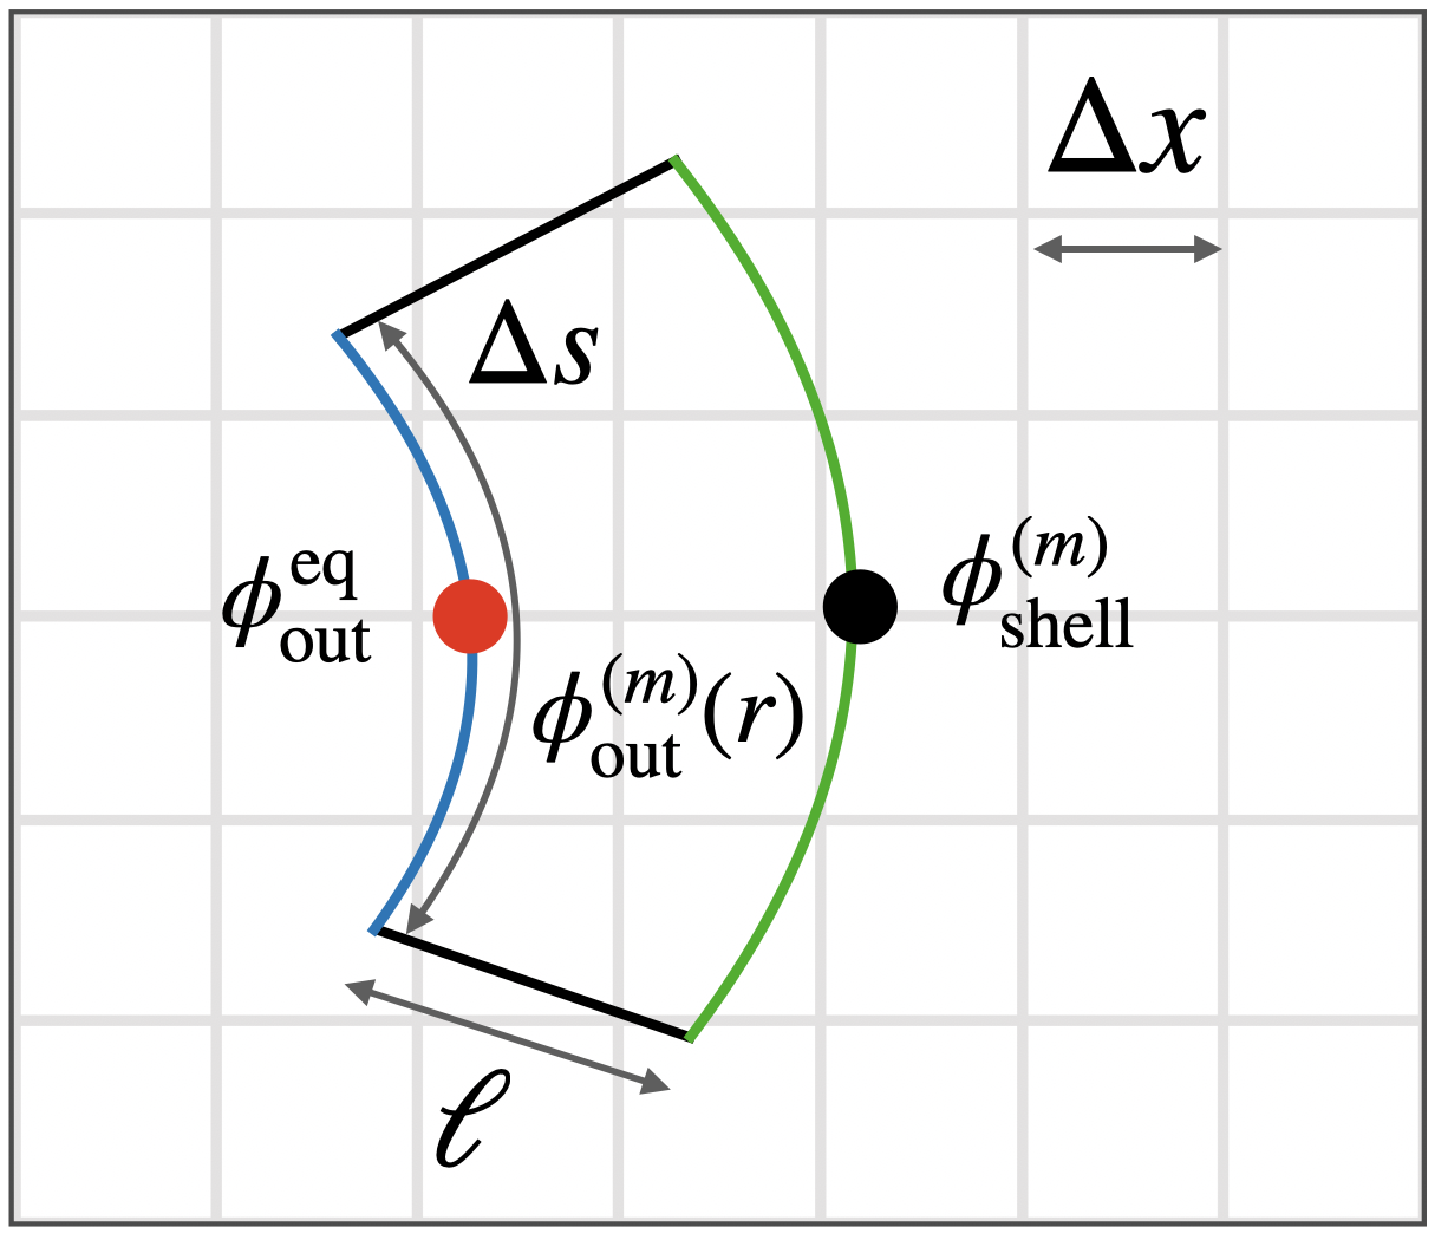
\includegraphics[scale=0.27]{MainContent/Figures/schematics_simulation_parameters.pdf}
\caption{
\textbf{Simulation parameters $\dx, \ell, \ds$ in the effective droplet model shown in a shell sector.}
$\dx$ is the resolution of the discretized background field $\phiOut$ and is an important parameter to capture it's dynamics described by \Eqref{eqn:RD_dilute}. 
$\ell$ and $\ds$
discretize the vicinity of the droplet into $N$ uniformly chosen sectors.
We solve for $\phiOut^{(m)}(r)$ inside the $m$-th shell sector from \Eqref{eqn:phi_out_in_shell} using the boundary conditions $\phiOut^{(m)}(R) = \phiEqOut$ and $\phiOut^{(m)}(R + \ell) = \phiShell^{(m)}$, which is estimated from a linear interpolation of the discretized background field $\phiOut$.
We then evaluate the fluxes $\jIn$; see \Eqref{eqn:flux_inside}, and $\jOut$; see Appendix \ref{sec:fluxes_inside_shell}, to calculate dynamics of droplets described by \Eqsref{eqn:DropletDiscretized}. 
}
\label{fig:schematics_simulation_parameters}
\end{figure}

\section{Grid discretization $\dx$}

The spatial discretization $\dx$; (see Fig. \ref{fig:schematics_simulation_parameters}), determines the resolution at which spatial variations of the background field $\phiOut$ are resolved.
Consequently, the choice of $\dx$ is based on the physics of the problem:

\begin{enumerate}
    \item If spatial variation in $\phiOut$ is negligible and a mean-field model is desired, $\dx$ can be arbitrarily large so that $\phiOut$ can vary only in time and little in space.
    
    \item If spatial variation of $\phiOut$ between droplets are important, $\dx$ needs to be smaller or equal than the mean droplet separation to resolve droplet-droplet interactions mediated through the background field $\phiOut$.
    
    \item External gradients that affect droplets; see Refs. \cite{Review2019,Weber2017,Lee2013,Bressloff2020,Bressloff_2020} can also play a role in determining the resolution of $\phiOut$, as $\dx$ needs to be on the order of the droplet radii, so spatial anisotropies can be resolved on the droplet level.
\end{enumerate}
To summarize, several competing length-scales of interest can exist such as the mean droplet radius, mean droplet-droplet separation distance, external gradients, reaction-diffusion length-scales; see Ref. \cite{Review2019} at which the resolution of $\phiOut$ is desired. 
Consequently, we fix $\Delta x$ based on the length-scale at which the resolution of $\phi_{\mathrm{out}}$ is needed.

\section{Annular shell thickness $\ell$}

The most important part of the effective droplet model is how accurately material exchanges between the droplets and the background field $\phiOut$ are captured.
These material exchanges form the core of our numerical model, which allows us to `de-couple` droplets from the background field.
Recall that in the vicinity of each droplet, $\phiOut$ is altered as a consequence of it's existence.
To appropriately describe the fluxes outside the droplets, we interpolate the background field in an annular shell of thickness $\ell$ around the droplet, which is further discretized into $N$ uniformly chosen sectors.

The shell thickness $\ell$ (see Fig. \ref{fig:schematics_simulation_parameters}) thus plays a major role in calculating the fluxes outside the droplet $\jOut$; see Appendix \ref{sec:fluxes_inside_shell}, and an incorrect value for $\ell$ could potentially impact the growth and drift of droplets.
The thickness $\ell$ of the shell can thus be interpreted as an interpolation length-scale and its value affects the accuracy of the simulation as:

\begin{enumerate}

    \item If $\ell$ is too small, the fluxes $\jOut^{(m)}$ are overestimated since they scale with $\ell^{-1}$ (see Appendix \ref{sec:fluxes_inside_shell}).
    Additionally, it would lead to an underestimation of the effect the droplet has on altering $\phiOut$ in it's vicinity. 
    
    \item If $\ell \gg \dx$, the background field $\phiOut$ would not be evaluated in the vicinity of the droplet, so interactions close to the droplet cannot be estimated accurately.
    It would also imply that $\phiShell^{m}$ would be calculated far away from the droplet, leading to an erroneous representation of $\phiOut$ close to the droplet.  
    
\end{enumerate}
Taken together, we conclude that $\ell \sim \dx$ is a reasonable choice for the shell thickness and we later show that this choice works well.

\section{Shell sector width $\ds$}

To resolve spatial anisotropies of $\phiOut$ around the vicinity of a droplet, we discretize the shell of thickness $\ell$ into $N$ uniformly chosen sectors; see Fig. \ref{fig:schematics_simulation_parameters}.
Consequently, the discretization of the vicinity of the droplet is directly proportional to the number of shell sectors $N$, and a higher value for $N$  would potentially lead to a higher accuracy at the expense of larger computational cost.
Note that this implies that the dynamics of larger droplets will be described by more sectors to faithfully capture the interaction with their surrounding.

Similar to the shell thickness, $\ds$ also plays a role in accurately calculating the fluxes $\jOut^{(m)}$ in the vicinity of the droplet.
To obtain the correct estimates for $\jOut^{(m)}$, $\phiShell^{m}$ has to be calculated for the $m$-th shell sector by interpolating the background field $\phiOut$ once per shell sector.
The choice of $\ds$ affects the simulation in the following ways:

\begin{enumerate}
    \item $\Delta s \gg \Delta x$ leads to fewer points of exchange for each sector and an inaccurate estimate of material fluxes. 
    Additionally, it also results in under-resolving of potential heterogeneity of $\phiOut$ in the vicinity of the droplet, thus potentially affecting it's drift speed and position.
    
    \item The lower limit of $\ds$ is also limited by the background field discretization $\dx$, as increasing $N$ will have hardly any benefit, if the distance $\Delta$ between interpolation points is already smaller than $\dx$.
    For $d=2$ dimensions, $\Delta$ is roughly $\ds \approx 2\pi R/N$, and in $d=3$ dimensions, we define $\Delta$ as $\ds \approx\sqrt{4 \pi R^2 / N}$; see \figref{fig:schematics}B.

\end{enumerate}
Taken together, we again conclude that $\ds \sim \dx$ is a reasonable choice for the shell thickness, which we discuss next.
To summarize, we gave qualitative arguments towards the right choices for the simulation parameters, which for $\dx$ is the resolution of $\phiOut$ desired and for $\ell, \ds$ is $\ell \approx \ds \approx \dx$.

Next, we test our claim for the optimum choices of the simulation parameters by comparing our effective model to simulations using continuous model.
We use a test-case to investigate and quantify the effects of each simulation parameter. 
The test-case which we consider has to possess enough complexity so that changes in the simulation parameters have to sufficiently affect the dynamics of the droplets and the background field.
We hence need a test-case such that it possesses the following qualities:

\begin{enumerate}
    \item Heterogeneity in the background field $\phiOut$ to correctly capture it's dynamics, so that the accuracy of the choice for $\dx$ can be verified.

    \item Heterogeneity of $\phiOut$ in the vicinity of the droplets, so that the accuracy for the choice of $\ell, \ds$ can be verified.

\end{enumerate}
Our test case thus consists of two identical passive droplets, both of initial radius $R_0=20\,w$; where $w = 2 \sqrt{\kappa/b}$ (see Chapter \ref{chap:Chapter_2}), and whose centers are separated by $S_\mathrm{d}=10\,R_0$; see Fig. \ref{fig:droplet_pair_schematics}A.
The droplets are placed in a background of vanishing initial fraction, so the system is under-saturated and the droplets will shrink over time; see Fig. \ref{fig:droplet_pair_schematics}B.

For the continuous model, instead of simulating a 3 dimensional system which would be computationally expensive, we exploit the angular symmetry of the problem.
We consider an azimuthally symmetric cylindrical domain where $r,z \in [0, 682 w]$.
Conversely, our effective model is simulated in a $3$-dimensional cubic domain of size $L = [0, 1000 w]^{3}$.

\begin{figure}[tb]
\centering
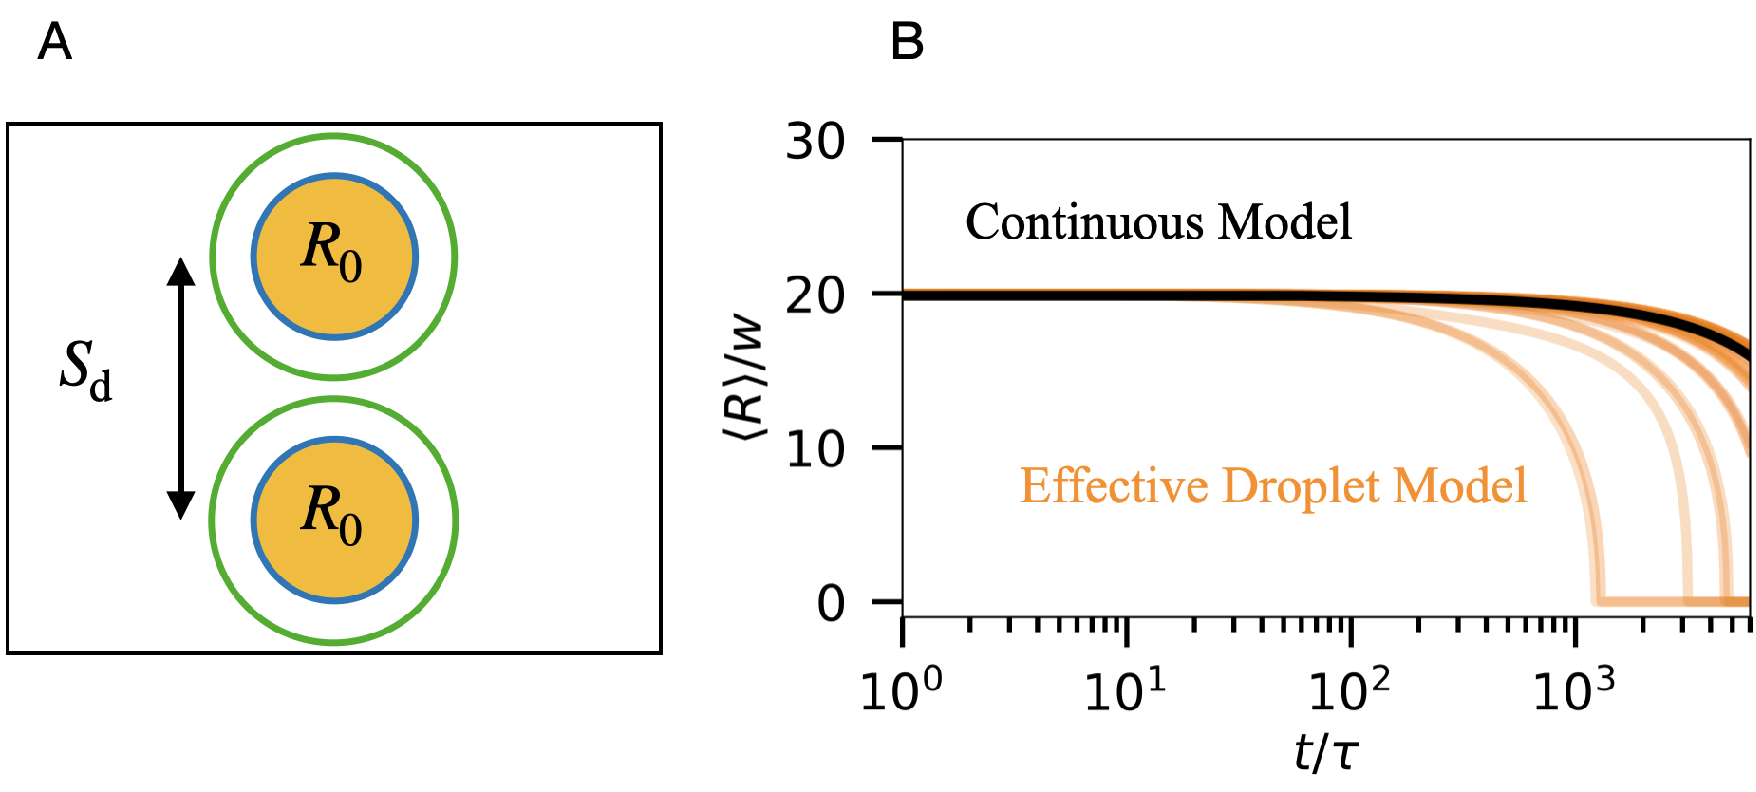
\includegraphics[scale=0.5]{MainContent/Figures/droplet_pair_schematic.pdf}
\caption{
\textbf{Schematics of the test-case (A) and typical behaviour of the effective droplet model for varying simulation parameters (B).}
(A) Two droplets with radii $R_0 = 20 w$ are placed with their centers $S_\mathrm{d} = 10 R_0$ apart in an empty background, $\phiOut(\vec{r}, t=0) = 0$, with their shells (in green).
(B) Mean droplet size $\langle R \rangle$ as a function of time for simulations using the continuous model (in black) and for varying simulation parameters for the effective droplet model (in orange).
$\langle R \rangle$ shows drastically different behaviour for some simulation parameters (orange lines) for the effective droplet model when compared to the continuous model (black line), thus highlighting the importance of choosing optimum values of simulation parameters for the effective droplet model.  
\mbox{(A, B)}
The continuous model simulations are performed in an azimuthally symmetric cylindrical domain of bounds $r,z \in [0, 682 w]$ with a spatial discretization of $0.5w$.
Effective simulations used a $3$-dimensional cubic domain of size $L = [0, 1000 w]^3$ with $l_{\gamma, \mathrm{in}} = 0.166 w$ and the simulation parameters were varied from uniformly choosing $\dx \in [0.5R_0, 10R_0], \ds \in [0.25R_0, 2R_0]$ and $\ell \in [0.5R_0, 5R_0]$.
Additional model parameters are $s=0$, $\Lambda = w^2 / b \, \tau$, $\phi^{(0)}_\mathrm{out} = 0$, $\phi^{(0)}_\mathrm{in} = 1$, $\tau = w^2/D_\mathrm{out}$, and $w = 2 \sqrt{\kappa / b}$.
}
\label{fig:droplet_pair_schematics}
\end{figure}

We first simulate the droplet pair using the continuous model for a duration $T$ after which the droplets typically have shrunk by about $20\%$.
We then simulate our effective droplet model for the same time $T$ and compare the final radii of the droplets from both the simulations. 
The deviation of the mean droplet radius $\mean{R_*}$ of our effective model compared to the radius $\mean{R_\mathrm{CM}}$ of the continuous model allows us to determine the crucial simulation parameters $\dx$, $\ell$, and $\ds$.

\section{$\dx \approx \ds \approx \ell$ is an optimum choice for the simulation parameters}

We first quantify the effects of changing the shell thickness $\ell$ on the accuracy of the simulation.
We keep the background field discretization $\dx \approx R_0$, as we aim to capture the interaction on a droplet level.  
\figref{fig:shell_parameters}A shows the final mean radii of the droplets $\langle R_\ast \rangle$ obtained from the effective droplet model and $\mean{R_\mathrm{CM}}$ (gray dashed line) obtained from the continuous model for $\dx \approx \ds$.
We see that the error is less than $\pm 5\%$  between $\langle R_\ast \rangle$ and $\mean{R_\mathrm{CM}}$ for the choice of $\ell \approx R_0$.
Similarly, we now fix $\dx \approx \ell$; see \figref{fig:shell_parameters}B and see that the error is less than $\pm 5\%$  between $\langle R_\ast \rangle$ and $\mean{R_\mathrm{CM}}$ for the choice of $\ds \approx R_0$.

\begin{figure}[tb]
\centering
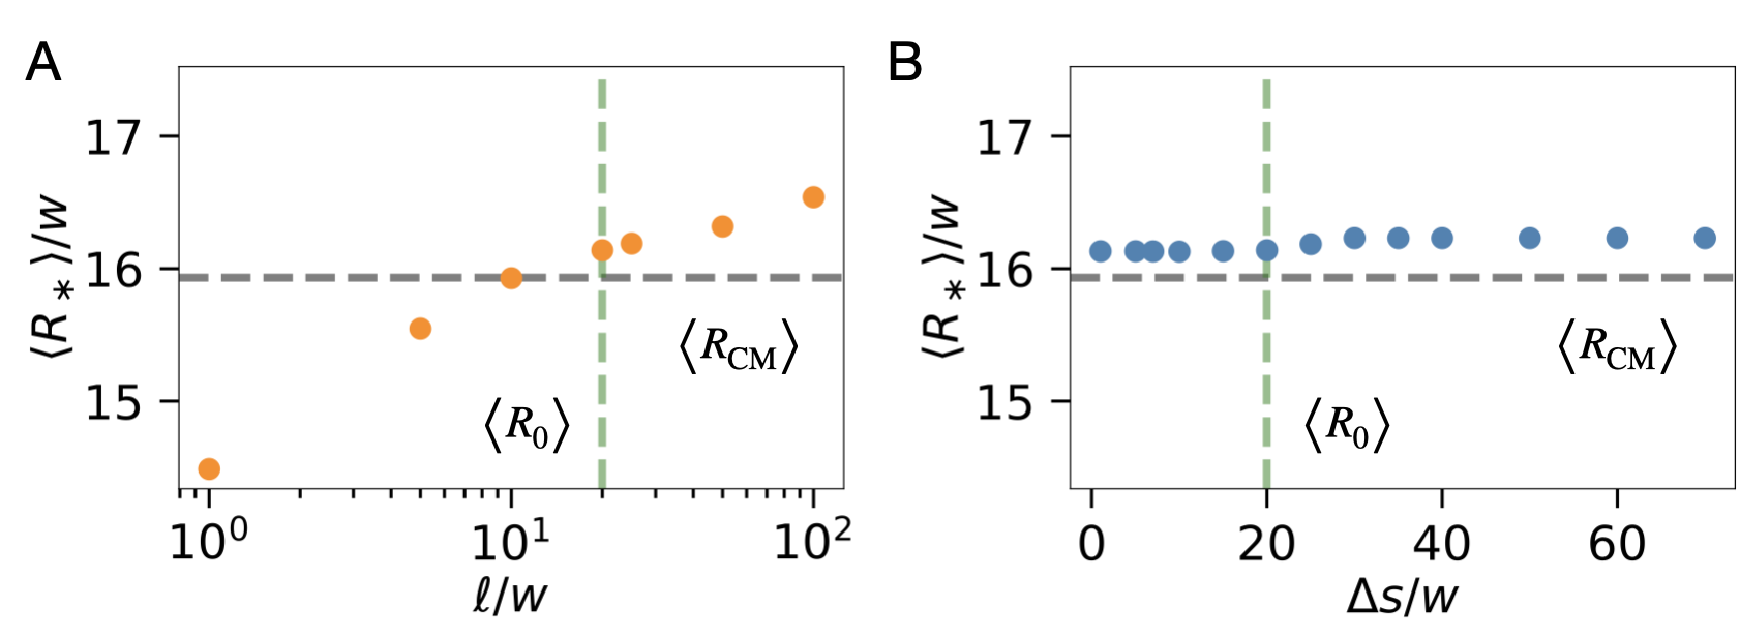
\includegraphics[scale=0.5]{MainContent/Figures/droplet_pair.pdf}
\caption{\textbf{Effect of shell thickness $\ell$ and sector size $\ds$ on simulations of a passive droplet pair.}
(A) Mean droplet size $\langle R_\ast \rangle$ as a function of $\ell$ (orange dots) for $\dx \approx \ds \approx R_0$ compared to the ground truth $\mean{R_\mathrm{CM}}$ (gray dashed line) obtained from the continuous model.
The choice $\ell \approx R_0$ (green dashed line) provides good agreement and the error between $\left \langle R_\mathrm{CM} \right \rangle$ (dotted grey line) and $\left \langle R_\ast \right \rangle$ is less than $\pm 5\%$.
(B) $\langle R_\ast \rangle$ as a function of $\ds$ (blue dots) for $\dx \approx \ell \approx R_0$ compared to $\mean{R_\mathrm{CM}}$, where the error between $\left \langle R_\mathrm{CM} \right \rangle$ (dotted grey line) and $\left \langle R_\ast \right \rangle$ is less than $\pm 5\%$.
Remaining parameters are specified in Fig. \ref{fig:droplet_pair_schematics}.
}
\label{fig:shell_parameters}
\end{figure}

Taken together, \figref{fig:shell_parameters} successfully shows that $\Delta x \approx \ell \approx \Delta s$ is a sensible choice for the parameters of our algorithm and leads to the best estimate of the droplet growth.
Finally, in order to ensure that our choice for the optimum parameters is independent of this particular test-case, we vary the initial radius of the droplets $R_0$ and their initial separation distance $S_\mathrm{d}$; see Appendix \ref{sec:RobustnessDropletPair}, as:

\begin{enumerate}
    \item $R_0 = 10w \mathrm{~and~} S_\mathrm{d} = 40w$.
    \item $R_0 = 10w \mathrm{~and~} S_\mathrm{d} = 100w$.
    \item $R_0 = 20w \mathrm{~and~} S_\mathrm{d} = 80w$.
\end{enumerate}

We follow the same procedure as before and simulate the droplet pair using the continuous model for a duration $T$ after which the droplets typically have shrunk by about $20\%$, then simulate our effective droplet model for the same time $T$ and compare the final radii of the droplets from both the simulations.

We report that our conclusion for the optimum choice of the simulation parameters largely remain unchanged with the above three test cases; see \figref{fig:robustness_test_case}, and hence we conclude that $\dx \approx \ds \approx \ell$ is an optimum choice for the simulation parameters, where $\dx$ is determined from the resolution of $\phiOut$ desired.
Finally the optimum time-step $\dt$ is then chosen using \Eqref{eqn:time_step} from the optimum set of parameters $[\dx, \ell, \ds]$.

To see how this choice of the optimum parameters affects accuracy and speed of the simulation, we present various simulation scenarios in the next chapter, which range from single droplets in an heterogeneous environment to droplet coarsening of large dilute emulsions.
We first simulate these systems with the effective droplet model using the optimum parameters and then show the effects of varying these parameters on droplet growth and drift. 

\section{Summary}

In Chapter \ref{chap:Chapter_3}, we formulated the numerical algorithm for the effective droplet model; given by (Algorithm \ref{alg:algorithm}), which evolved droplet dynamics according to \Eqsref{eqn:DropletDiscretized} and the background field volume fraction field $\phiOut$ according to \Eqref{eqn:RD_dilute}, with the time-step $\dt$ calculate from \Eqref{eqn:time_step}.

In this chapter, we discussed the various simulation parameters arising from the effective droplet model, namely $\dx, \ell, \ds$ and their effects on the simulation.
We then sought to find the values for optimum simulation parameters which best replicate droplet dynamics, when compared with simulations using the continuous model given by \Eqref{eqn:CHActive}.

We claimed that the optimum values for these simulation parameters are $\dx \approx \ell \approx \ds$.
To verify our claim, we simulated a synthetic test-case comprising of a pair of identical droplets shrinking in a vanishing background field. 

We first simulated the droplet pair using the continuous model for a duration $T$ after which the droplets typically had shrunk by about $20\%$.
We then simulated our effective droplet model for the same time $T$ and compared the final radii of the droplets from both the simulations.
The deviation of the mean droplet radius $\mean{R_*}$ of our effective model compared to the radius $\mean{R_\mathrm{CM}}$ of the continuous model allowed us to determine the optimum values of the simulation parameters which most faithfully model droplet dynamics as $\dx \approx \ell \approx \ds$ ; see \figref{fig:shell_parameters} and \figref{fig:robustness_test_case}.
\clearpage

% Chapter 5

\onehalfspacing

\chapter{Comparison with known literature}

\label{chap:Chapter_5}

Until now we elaborated on the development of the numerical algorithm for the effective droplet model.
This model is built from the thin-interface approximation of the continuous model \Eqref{eqn:CHActive} and evolves the dynamics of the droplets via \Eqsref{eqn:DropletDiscretized} and dynamics of the background field $\phiOut$ using \Eqref{eqn:RD_dilute}.
We then laid out a procedure for choosing the optimum values for the various simulation parameters $\dx, \ell, \ds$ by comparing simulations of a test-case with the ground-truth i.e simulations using the continuous model.
We then arrived at the conclusion that $\dx \approx \ell \approx \ds$ is indeed an optimum choice for the simulation parameters, and finally the time-step $\dt$ is chosen from \Eqref{eqn:time_step} using the optimum values for $[\dx, \ell, \ds]$. 

We now demonstrate that the effective droplet model accurately captures the dynamics of the droplets and the background field in diverse scenarios, using the optimum values for the simulation parameters.
In Chapter \ref{chap:Introduction}, we discussed how biological cells use a setup featuring external chemical gradients and chemical reactions to control the position of droplets in their interior.
We cite a few more examples to put the point across. 

Rai et al. \cite{Rai2018} showed that during mitosis, an enzyme known as DYRK3 dissolves only selected condensates but keeps others such as P-bodies and nucleoli untouched, to prevent aberrant condensation.
The same kinase (DYRK3) is also known to dissolve stress granules during stress recovery, as shown by Wippich et al. \cite{Wippich2013}.
Brangwynne et al. \cite{Brangwynne2009} in their seminal work showed that P-granules localize to the posterior side in early stage \textit{C. elegans} embryos, which is governed by a gradient of a protein known as MEX-5.
On similar lines, Griffin et al. \cite{Griffin2011} showed how phosphorylation and dephosphorylation reactions generate concentration gradients throughout the cytoplasm.
Weber et al. \cite{Weber2017} utilized theory and simulations to explore the influence of chemical gradients on phase separation, thus shedding insights into how cells utilize local concentration gradients to spatially organize biomolecular condensates in their cytoplasm.

However, the cell also has to spatially control the ripening of condensates and preventing them from aggregating together and forming bigger droplets, which can happen due to Brownian mediated coalescence or \textit{Ostwald-Ripening}; see Refs. \cite{Review2019,Weber2017}.
Brownian mediated coalescence requires droplets to be physically close to each other, where they merge into bigger droplets upon contact. 
On the other hand, \textit{Ostwald-Ripening} is governed by gradients of chemical potential arising between the droplets as a result of unequal equilibrium volume fractions, due to heterogeneity in their size.
Generally, the cytoplasm inside the cell can show visco-elastic properties; see Ref. \cite {Xie2022}, which might lead to a slow ripening of the condensates.
Weiss et al. \cite{Weiss2004} also demonstrated that condensates can be strongly influenced by the cytoskeleton, and anomalous diffusion can arise due to molecular crowding, thus adversely affecting larger condensates and in turn not affecting diffusion across smaller condensates as much.
Thus, in this thesis, we will focus on \textit{Ostwald-Ripening} and we will not consider Brownian mediated coalescence. 

In the following section, we demonstrate that the effective droplet model is able to simulate two mechanisms (out of many), which the cell potentially uses to regulate the dynamics of condensates - in particular, chemical reactions and external chemical gradients.
To help disentangle the individual roles of these two mechanisms and to study how they affect dynamics of phase separated droplets, we consider them separately: first in simulations of single droplet systems, and then simulations of many droplet systems. 

We start by considering a simple scenario of a single passive droplet growing when immersed in a supersaturated background field.
We compare droplet growth using the effective droplet model, simulations using the continuous model and analytical results.
We then slowly build up complexity by adding chemical reactions and chemical gradients and more droplets; comparing them with simulations using the continuous model (wherever computationally possible) and analytical predictions, eventually reaching the situation where we simulate the coarsening dynamics of hundreds of droplets using the effective droplet model, as the continuous model is computationally expensive to be simulated.

\section{Passive droplet in a large background field}
We start by considering the simplest case of a passive droplet immersed in a large background field $\phiOut$.
We immerse the droplet in an initial volume fraction $\phi_\infty$ much greater than it's equilibrium volume fraction $\phiEqOut$, so the droplet grows in time. 
We demonstrate that the effective droplet model captures the growth of the droplet accurately when compared with simulations using the continuous model and analytical predictions.

As the droplet experiences an isotropic environment, the fluxes $\jOut$ entering the droplet from the background field will be isotropic in all directions, and hence the droplet will only grow and not drift; see \Eqsref{eqn:DropletDiscretized}.
We next derive the volume fractions inside and outside the droplet $\phiIn,~\phiOut$ analytically, enabling us to calculate the material fluxes $\jIn,~\jOut$, leading to droplet growth.

\subsection{Volume fraction profile and material fluxes inside the droplet}
Owing to symmetry, we place a spherically symmetric co-ordinate system at the centre of the droplet with $r$ being the radial co-ordinate.
Since $\phiIn$ inside the droplet typically varies only a little, we use the thin-interface approximation; see \Eqsref{eqn:thin_interface_model}, of the continuous model to approximately arrive at the dynamical equation for $\phiIn$ as:

\begin{align} 
    \label{eqn:RD_droplet_passive}
    \frac{\partial \phiIn}{\partial t}
        \approx D_\mathrm{in} \nabla^2 \phiIn,
\end{align}
where $D_\mathrm{in}$ is the diffusivity inside the droplet.
We invoke the standard \textit{quasi-static approximation} and assume that the droplet radius changes on a timescale which is much slower than the transients in \Eqref{eqn:RD_droplet_passive}; see Ref. \cite{Review2019}.

We can then analytically solve for $\phiIn$ from the stationary state of \Eqref{eqn:RD_droplet_passive}, using the boundary conditions $\phiIn(R) = \phiEqIn$ and $\partial_r \phiIn (0) = 0$ and we thus obtain a constant volume fraction inside the droplet as $\phiIn(r) = \phiEqIn$.

\subsection{Volume fraction profile and material fluxes outside the droplet}

Similar to inside the droplet, the volume fraction inside in the background field $\phiOut$ also typically varies a little and is hence described from the thin-interface approximation; see \Eqsref{eqn:thin_interface_model}, as:

\begin{align} 
    \label{eqn:RD_dilute_passive}
    \frac{\partial \phiOut}{\partial t}
        \approx D_\mathrm{out} \nabla^2 \phiOut,
\end{align}
where $D_\mathrm{out}$ is the diffusivity outside the droplet.
We solve for $\phiOut$ from the stationary state of \Eqref{eqn:RD_dilute_passive} using the boundary conditions $\phi_\mathrm{out}(R) = \phiEq_\mathrm{out}$ and far from the droplet $\phi_\mathrm{out}(\infty) = \phi_\infty$.
We thus obtain the volume fraction profile outside the droplet as $\phiOut(r) = \phi_\infty + (\phiEqOut - \phi_\infty) (R/r)$ and solution thus reveals that $\phiOut$ will monotonically approach $\phi_\infty$. 

\subsection{Material flux balance and droplet growth rate}

Spatial gradients in $\phiIn$ and $\phiOut$ lead to local material fluxes outside the droplet as $\vec{j}_\mathrm{out} \cdot \vec{n} = [-D_\mathrm{out} {\boldsymbol{\nabla}} \phiOut (R)] \cdot \vec{n} = -D \left[ \phi_{\infty}/R  - \phiEqOut / R \right]$, and inside the droplet as $\vec{j}_\mathrm{in} \cdot \vec{n} = [-D_\mathrm{in} {\boldsymbol{\nabla}} \phiIn (R)] \cdot \vec{n} = 0$.
Note that, we typically assume same diffusivity $D$ inside and outside the droplets, i.e. $D_\mathrm{out} \approx D_\mathrm{in} = D$.
The interfacial speed $v_n$ is calculated from
\Eqref{eqn:InterfacialSpeed}, and we can calculate the droplet growth rate from \Eqref{eqn:DropletGrowth} as:
\begin{equation}
	\label{eqn:interfacefluxes_passive}
	\frac{\mathrm{d} R}{\mathrm{d} t} = \frac{1}{S} \int_{\Omega} v_n ~ \mathrm{d}A = D\left ( \frac{\phi_{\infty}}{R}  - \frac{\phiEqOut}{R} \right ),
\end{equation}
where $S$ is the surface area of the droplet, $\Omega$ is the droplet surface and $\mathrm{d} A$ is the area element on the droplet surface.
Note that the only solution for ${\mathrm{d} R}/{\mathrm{d} t} = 0$ from \Eqref{eqn:interfacefluxes_passive} is $R_{\ast}$ (as $\phiEqIn,~\phiEqOut$ depend on the droplet radius $R$; see \Eqsref{eqn:GibbsThompsonRelations}). Droplets smaller than the critical radius $R_{\ast}$, defined as the radius at which the equilibrium volume fraction of the droplet equals the local supersaturation, dissolve quickly and is hence an unstable radius.

Having calculated the droplet growth rate analytically, we validate our choices for the optimum simulation parameters for the effective droplet model by simulating a single passive droplet of radius $R_0 = 2w$ embedded in a large supersaturated background field of value $\phiOut(t = 0) = \phi_\infty = 0.1$.
The droplet grows over time by ingesting material from the surroundings, as $\phiEqOut < \phi_\infty$.

Exploiting the symmetry of the problem, the continuous model uses a spherically symmetric domain of size $r \in [0, 400 w]$ and the effective droplet model uses a 3 dimensional periodic domain of size $[-L, L]^3$ with $L = 322 w$ with optimum simulation parameters $(\dx \approx \ell \approx \ds \approx R_0)$. Fig. \ref{fig:passive_droplet} shows a good agreement with the analytical prediction from \Eqref{eqn:interfacefluxes_passive} and the continuous model.

\begin{figure}[tb]
\centering
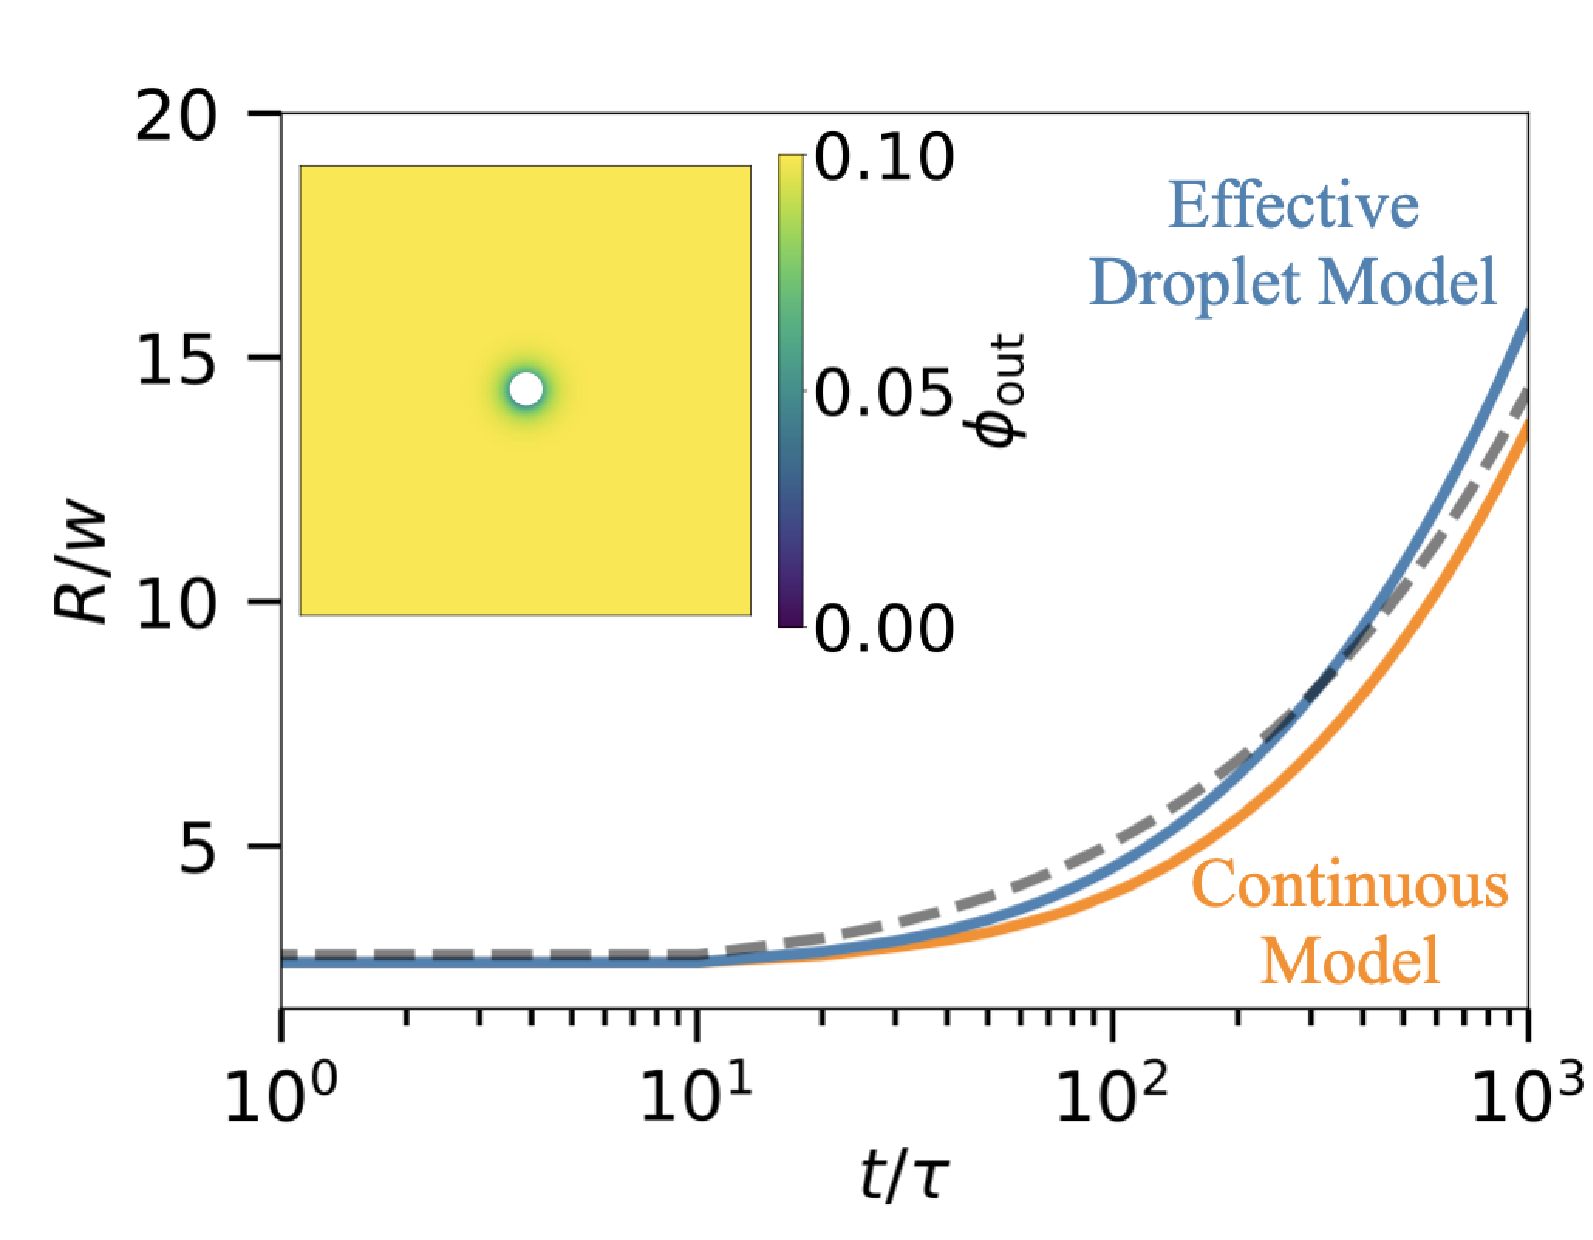
\includegraphics[scale=0.4]{MainContent/Figures/single_passive_droplet_growth.pdf}
\caption{
\textbf{Passive droplet growing when immersed a large supersaturated background field.}
Droplet radius $R$ as a function of time $t$ when immersed in a uniform supersaturation of volume fraction $\phi_\infty$.
Simulations using the effective droplet model with optimum parameters (blue line) matches well with analytical prediction from \Eqref{eqn:interfacefluxes_passive} (dashed line) and simulations using the continuous model (orange line).
Inset shows the simulation snapshot at $t = 10^3 \tau$ from the effective droplet model, with the droplet (in white) and the background field $\phiOut$ reaching $\phi_\infty = 0.1$ far from the droplet.
The continuous model uses a spherically symmetric domain with $r \in [0, 400 w]$ along with periodic boundary conditions and $\phi(\vec{r}, t=0) = \phi_\infty$.
The effective model uses a $3$-dimensional periodic domain of size $[-L, L]^3$ with $L = 322 w$, $\phiOut(\vec{r}, t=0) = \phi_\infty$, $\dx \approx \ell \approx \Delta s \approx R_0$ and periodic boundary conditions.
Remaining parameters are specified in Fig. \ref{fig:droplet_pair_schematics}.
}
\label{fig:passive_droplet}
\end{figure}

We next focus on a slightly complex situation where a passive droplet is immersed in a gradient of the droplet material.
Note that in this case, the droplet experiences a local a non-isotropic environment and may potentially drift in space.

\section{Passive droplet in an external volume fraction gradient}

Earlier studies by Weber et al. \cite{Review2019,Weber2017} have considered two-component phase separation with the inclusion of a third (inert) component called the regulator, which maintains an external gradient of the equilibrium volume fraction throughout the system.
Since we focus on a binary system, we impose a volume fraction gradient of the droplet material via appropriate boundary conditions.
Similar to the previous case of passive droplet, we again derive analytical predictions for the growth and drift of such a droplet using the thin-interface approximation and compare them with simulations performed using the continuous model and with the effective droplet model using the optimum parameters. 
We will first derive $\phiIn,~\phiOut$, enabling us to calculate the material fluxes $\jIn,~\jOut$, enabling us to predict droplet growth and drift.
Consider an isolated passive droplet of radius $R$ with a spherical co-ordinate system centred at the droplet position $\vec{x_0}$. 
The volume fraction outside the droplet can thus be expressed as $\phiOut(r, \theta, \varphi)$, where $r$ is the radial distance from the centre of the droplet and $\theta \in [0, 2 \pi), \varphi \in [0, \pi]$ are the polar and azimuthal angles.
Without loss of generality, we assume that the droplet experiences a one dimensional gradient that varies along the $x$-coordinate as seen from \figref{fig:drop_in_gradient_schematic}.

In general, a position dependant supersaturation outside the droplet might lead to non-spherical droplets and possible deformations in their shapes. 
However, in this thesis, we focus solely on spherical droplets by assuming that a large surface tension $\gamma$ quickly nullifies any deformations in droplet shape.

Contrary to the case of a passive droplet in a supersaturated medium, the droplet here experiences a volume fraction $\phi_{\infty}$, which far from the droplet reads as $\phi_{\infty} = \alpha + \beta \, r \, \text{cos}\,\varphi$ because of the existence of the external gradient; see \figref{fig:drop_in_gradient_schematic}.
Here $\alpha, \beta$ are the mean volume fraction and strength of the gradient respectively at the position of the droplet. 

\begin{figure}[tb]
\centering
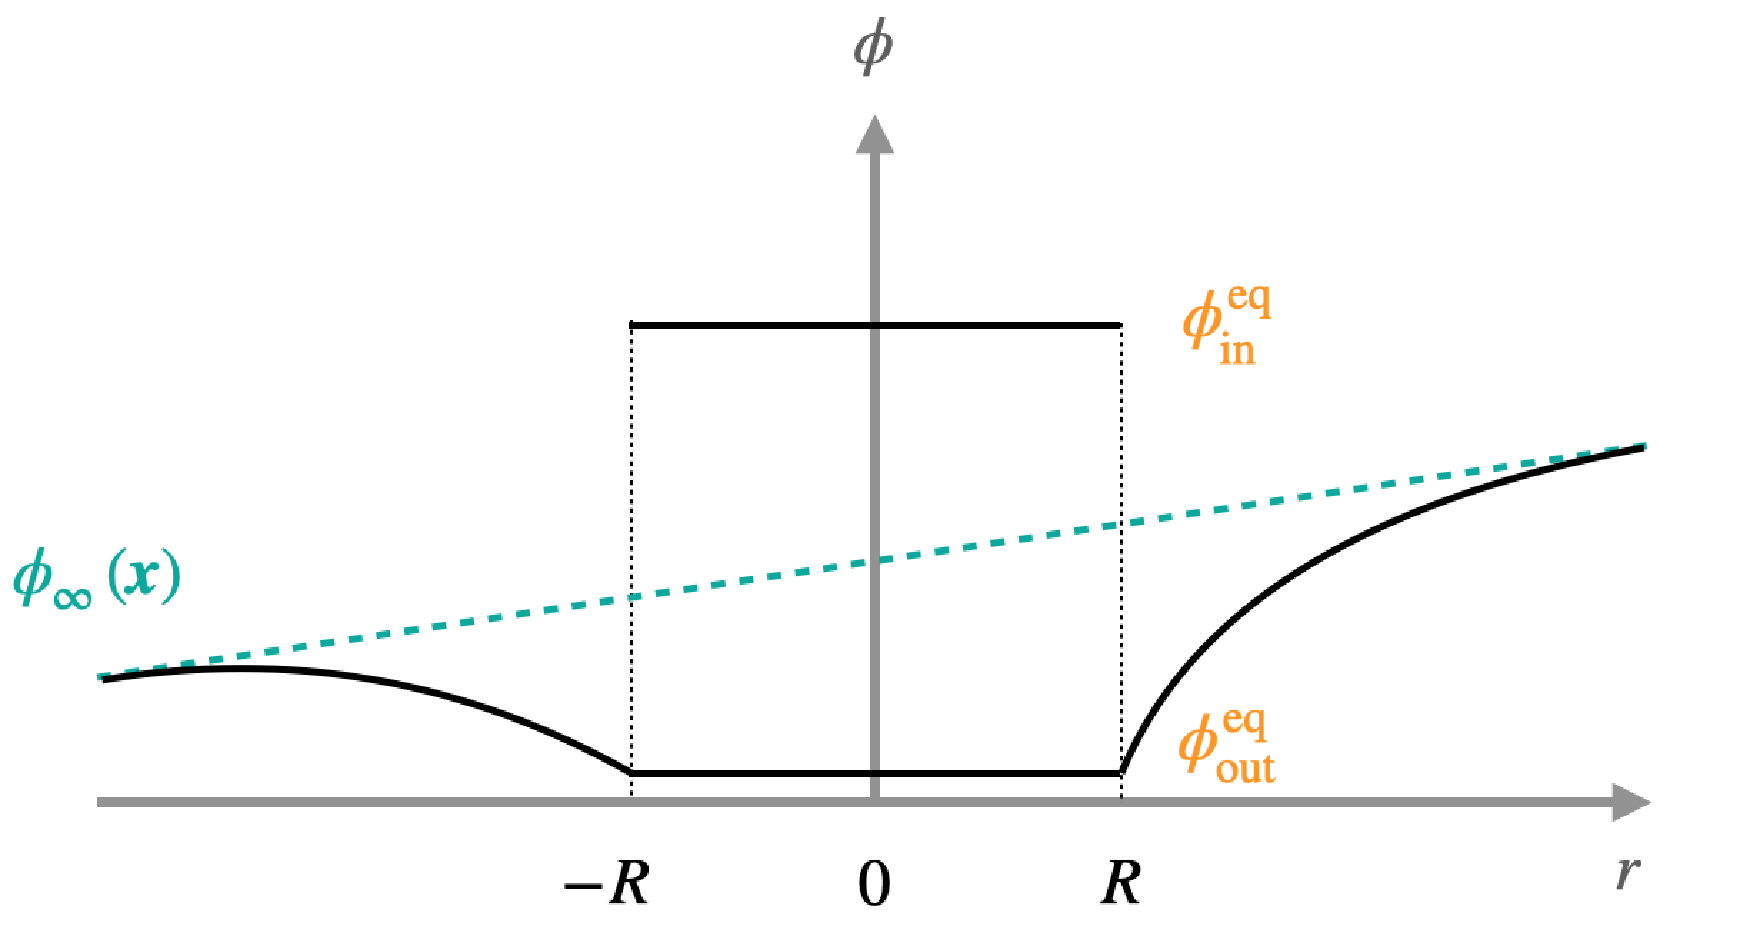
\includegraphics[scale=0.4]{MainContent/Figures/drop_in_gradient_schematic.pdf}
\caption{\textbf{Schematics of volume fractions inside and outside of a passive droplet immersed in an external volume fraction gradient.}
A droplet of radius $R$ at location $\vec{x} = 0$ is placed in a position dependant volume fraction $\phi_\infty (\vec{x})$.
$\phiEqIn,~\phiEqOut$ are volume fractions inside and outside the interface, given by \Eqsref{eqn:GibbsThompsonRelations}.
}
\label{fig:drop_in_gradient_schematic}
\end{figure}

We invoke the thin-interface approximation; see \Eqsref{eqn:thin_interface_model}, and as $\phiIn$ inside the droplet typically varies only a little, we solve for $\phiIn$ from the steady state of \Eqref{eqn:RD_droplet_passive}, using the boundary conditions $\phiIn(R) = \phiEqIn$ and $\partial_r \phiIn (0) = 0$ to obtain $\phiIn(r) = \phiEqIn$.
Similar to inside the droplet, the volume fraction inside in the background field $\phiOut$ also typically varies a little; see \Eqsref{eqn:thin_interface_model}, and can be solved from \Eqref{eqn:RD_droplet_passive} using the boundary conditions $\phi_\mathrm{out}(R) = \phiEq_\mathrm{out}$ and far from the droplet $\phi_\mathrm{out}(\infty) = \phi_{\infty} = \alpha + \beta \, r \, \text{cos}\,\varphi$.
We thus obtain the volume fraction profile outside the droplet as:
\begin{equation*}
    \phiOut(r, \varphi) = \alpha \left ( 1 - \frac{R}{r} \right ) + \beta \, \text{cos} \varphi \left ( r - \frac{R^3}{r^2} \right ) + \phiEqOut\,\frac{R}{r}.
\end{equation*}
We evaluate the local fluxes at the droplet surface as:
\begin{subequations}
\begin{align}
    \jIn \cdot \vec{n} &= [-D {\boldsymbol{\nabla}} \phiIn (R)] \cdot \vec{n} = 0 \mathrm{~and~} \nonumber
    \\[10pt]
    \jOut \cdot \vec{n} &= [-D {\boldsymbol{\nabla}} \phiOut (R)] \cdot \vec{n} = -D \left ( 3 \beta \text{cos} \varphi  + \frac{\alpha}{R} - \frac{\phiEqOut}{R} \right ), \nonumber
\end{align}
\end{subequations}
where we assume equal diffusivities inside and outside the droplet.
Note that $\jOut \cdot \vec{n}$ has an angular dependence, and hence the droplet will drift as a result of unequal fluxes on it's surface.
We then calculate the interfacial speed $v_n$ from \Eqref{eqn:InterfacialSpeed} and arrive at the droplet growth and drift speed along the $x$ co-ordinate from \Eqref{eqn:DropletGrowth} and \Eqref{eqn:DropletDrift} as:

\begin{subequations}
\label{eqn:interfacefluxes_gradient}
\begin{align}
	\frac{\mathrm{d} R}{\mathrm{d} t} &= \frac{1}{4 \pi} \int_{\Omega} D \left ( 3\,\beta \, \text{cos} \, \varphi  + \frac{\alpha}{R} - \frac{\phiEqOut}{R} \right ) \mathrm{d}A = \frac{D\,\alpha}{R} - \frac{D \phiEqOut }{R}
	\text{~and}
\\[10pt]
    \frac{\mathrm{d} x_0}{\mathrm{d} t} &= \frac{3}{4 \pi} \int_{\Omega} D \left ( 3\,\beta \, \text{cos} \, \varphi  + \frac{\alpha}{R} - \frac{\phiEqOut}{R} \right ) \text{cos} \, \varphi \, \mathrm{d}A = 3 D \beta,
\end{align}
\end{subequations}
where $\Omega$ is the droplet surface and $\mathrm{d} A$ is the area element on the droplet surface. 
Note that the drift speed is a constant value depending only on the strength of the gradient $\beta$ and the diffusivity $D$.
Naturally, increasing $\beta$ would lead to higher drift speeds for a constant diffusivity.

Having calculated the droplet growth rate and drift speed  analytically, we validate our choices for optimum parameters for the effective droplet model. 
We simulate a single passive droplet of initial radius $R_0 = 20w$ immersed in a linear volume fraction gradient of the droplet material maintained via appropriate boundary conditions. 
Similar to the case of the passive droplet growing in a supersaturated medium, the passive droplet in this case also grows over time by taking material from the surroundings. 
Furthermore, as $\jOut \cdot \vec{n}$ has a angular dependence, it results in unequal fluxes leading to droplet drift along the gradient.

Depending on the strength of the gradient $\beta$, we demonstrate that the effective droplet model captures droplet dynamics in both situations - for high and low value of $\beta$.
We first consider the case of high $\beta = 8.3 \times 10^{-5} w^{-1}$, as shown in Fig. \ref{fig:drop_in_gradient}A and Fig. \ref{fig:drop_in_gradient}B.
The continuous model uses a cylindrical domain with $r \in [0, 400 w]$, $z\in [-L_1, L_1]$ with $L_1=600 w$, azimuthal symmetry, and boundary conditions $\mu(z=-L_1) = 0$ and $\mu(z=L_1)= 0.072\,b w^3$ to impose the gradient.
Note that imposing a condition on the chemical potential $\mu$ means that the system can be assumed to be coupled to infinite reservoirs at it's $z$-boundaries, which enables us to maintain the gradient of the volume fraction field $\phi$ throughout the system. 
The effective model uses a $3$-dimensional box of size $[-L_2, L_2]^3$ with $L_2 = 422 w$, $\dx \approx \ell \approx \Delta s \approx R_0$, and boundary conditions $\phiOut(y = -L_2) = 0.01483$ and $\phiOut(y = L_2) = 0.0851$.
Fig. \ref{fig:drop_in_gradient}B shows a good agreement with the analytical predictions for droplet growth and drift from \Eqsref{eqn:interfacefluxes_gradient} and simulations using the continuous model.
We then consider the scenario with low $\beta = 4.2 \times 10^{-5} w^{-1}$, as shown in Fig. \ref{fig:drop_in_gradient}C and Fig. \ref{fig:drop_in_gradient}D.
The continuous model for this case uses the same parameters as the case with high $\beta$, but with boundary conditions $\mu(z=-L_1) = 0$ and $\mu(z=L_1)= 0.0427\,b w^3$ to impose the gradient.
The effective model uses the same parameters as the case with high $\beta$, but with boundary conditions $\phiOut(y = -L_2) = 0.007$  and $\phiOut(y = L_2) =  0.042$.
Fig. \ref{fig:drop_in_gradient}D also shows a good agreement with the analytical predictions for droplet growth and drift from \Eqsref{eqn:interfacefluxes_gradient} and simulations using the continuous model.

Additionally, it is interesting to see that increasing approximations of the continuous model (in orange) lead to increasingly worse estimates for droplet drift, as the analytical predictions from the thin-interface approximation (dashed line); see \Eqsref{eqn:thin_interface_model}, are approximations of the continuous model, and the effective droplet model (in blue) is an approximation of \Eqsref{eqn:thin_interface_model}.
Finally, note that the match for the droplet drift speed, given by $(\mathrm{d} x_0 / \mathrm{d} t = 3 D \beta)$ in three dimensions, gets worse for increasing $\beta$, which is expected, as seen from Fig. \ref{fig:drop_in_gradient}B and Fig. \ref{fig:drop_in_gradient}D.

\clearpage

\begin{figure}[tb]
\centering
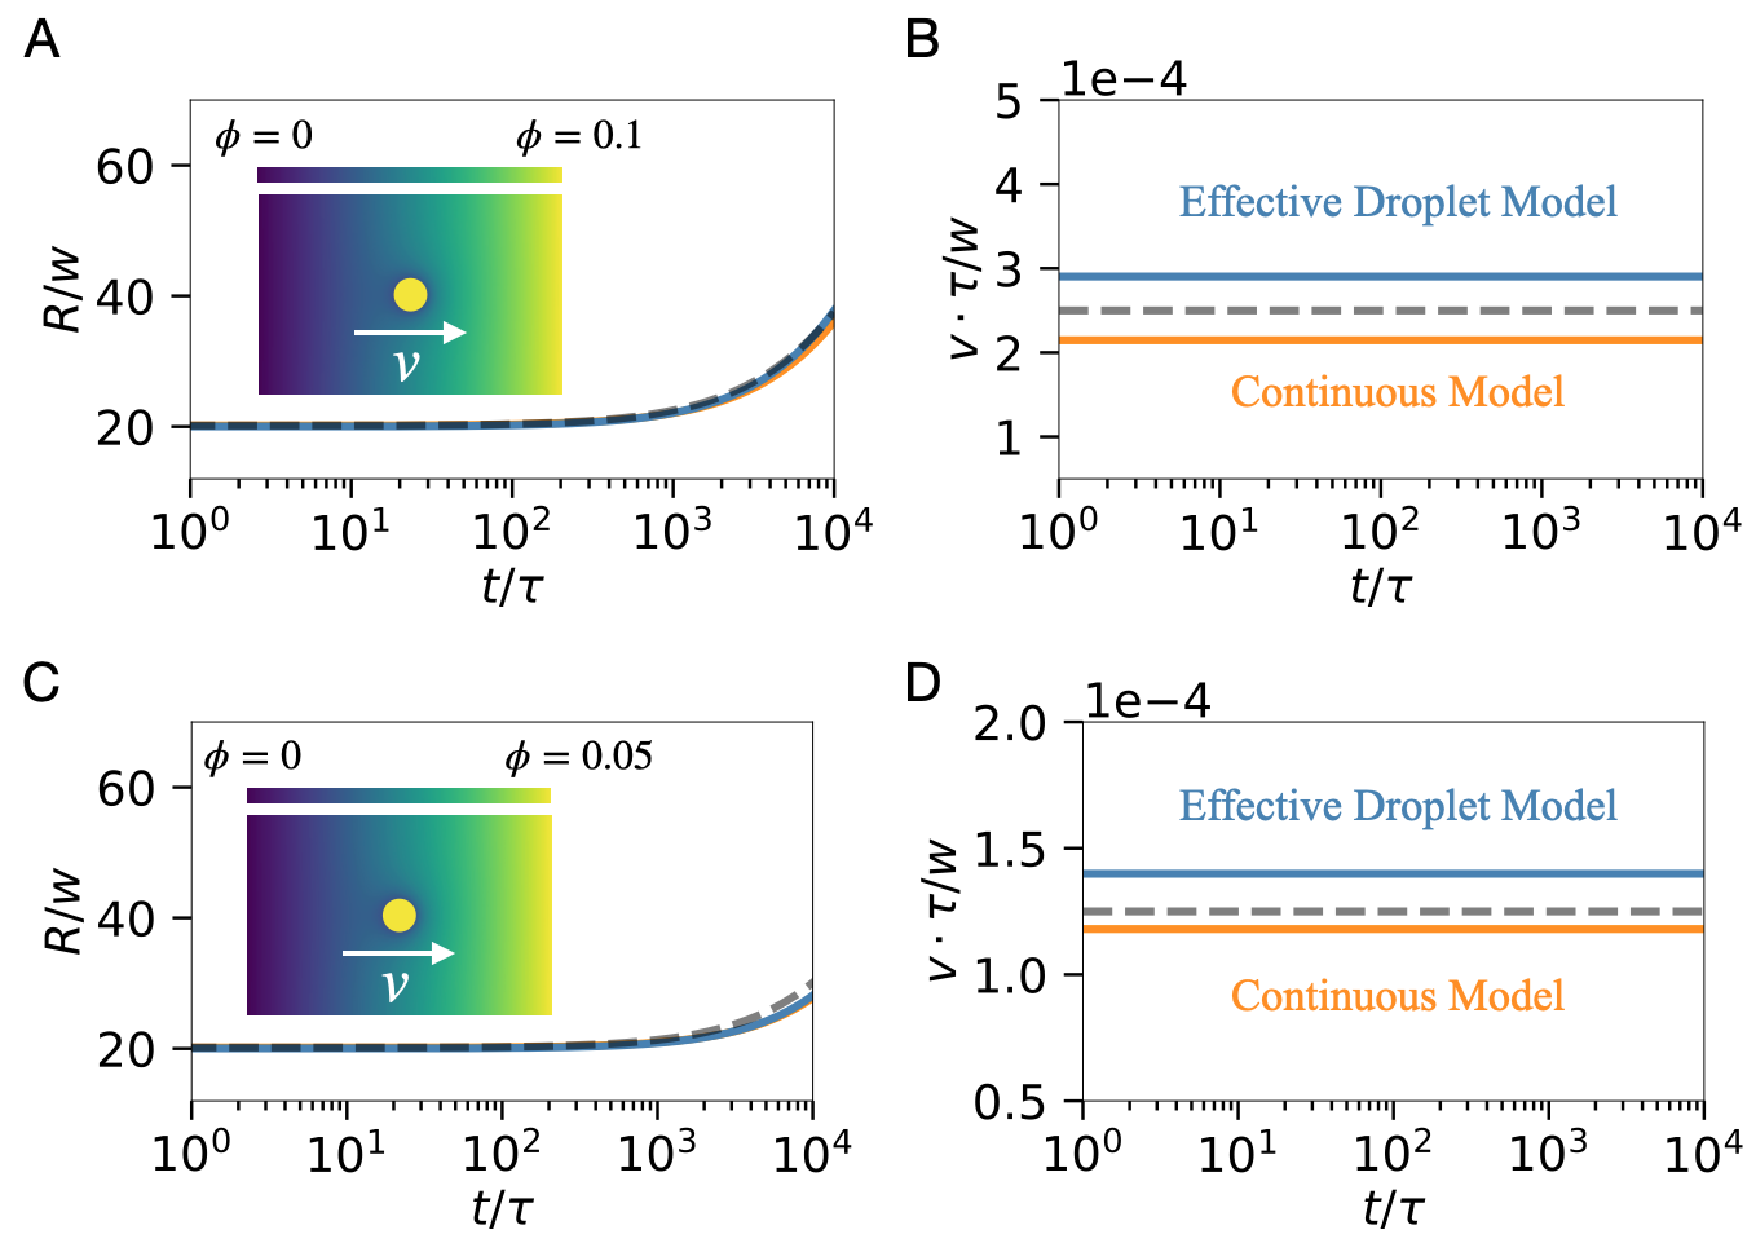
\includegraphics[scale=0.5]{MainContent/Figures/drop_in_gradient.pdf}
\caption{
\textbf{Droplet dynamics in external gradients.}
(A) Droplet radius $R$ as a function of time $t$ for the effective droplet model (blue), analytical prediction (dashed line) and the continuous model (orange).
The inset shows a schematic of the simulation with the strong gradient of droplet material imposed in the background.
(B) Droplet drift speed $v$ as function of $t$.
\mbox{(C, D)} Droplet radius $R$ and drift speed $v$ versus time $t$ for a weak gradient. 
\mbox{(A, B)}
The continuous model uses a cylindrical domain with $r \in [0, 400 w]$, $z\in [-L_1, L_1]$ with $L_1=600 w$ and azimuthal symmetry along with the boundary conditions $\mu(z=-L_1) = 0$ and $\mu(L_1)= 0.072\,b\,w^3$ to maintain the gradient throughout the system.
The effective model uses a $3$-dimensional box of size $[-L_2, L_2]^3$ with $L_2 = 422 w$, $\dx \approx R_0$, $\ell \approx \Delta s \approx R_0$ along with the boundary conditions $\phiOut(y = -L_2) = 0.01483$ and $\phiOut(y = L_2) = 0.0851$.
\mbox{(C, D)}
To maintain the gradient throughout the system, the continuous model uses the boundary conditions $\mu(z=-L_1) = 0$ and $\mu(z = L_1)= 0.0427\,b\,w^3$ and the effective droplet model uses the boundary conditions $\phiOut(y = -L_2) = 0.007$ and $\phiOut(y = L_2) = 0.042$ with the remaining parameters same as \mbox{(A, B)}.
Note that in the absence of droplets, boundary conditions imply identical linear gradient in the continuous model as $\phi = \phi(z)$ and in the effective droplet model as $\phiOut = \phiOut(y)$, which were also used to initialize the background for both the models.
Remaining parameters are specified in Fig. \ref{fig:droplet_pair_schematics}.
}
\label{fig:drop_in_gradient}
\end{figure}

\clearpage

\begin{figure}[tb]
\centering
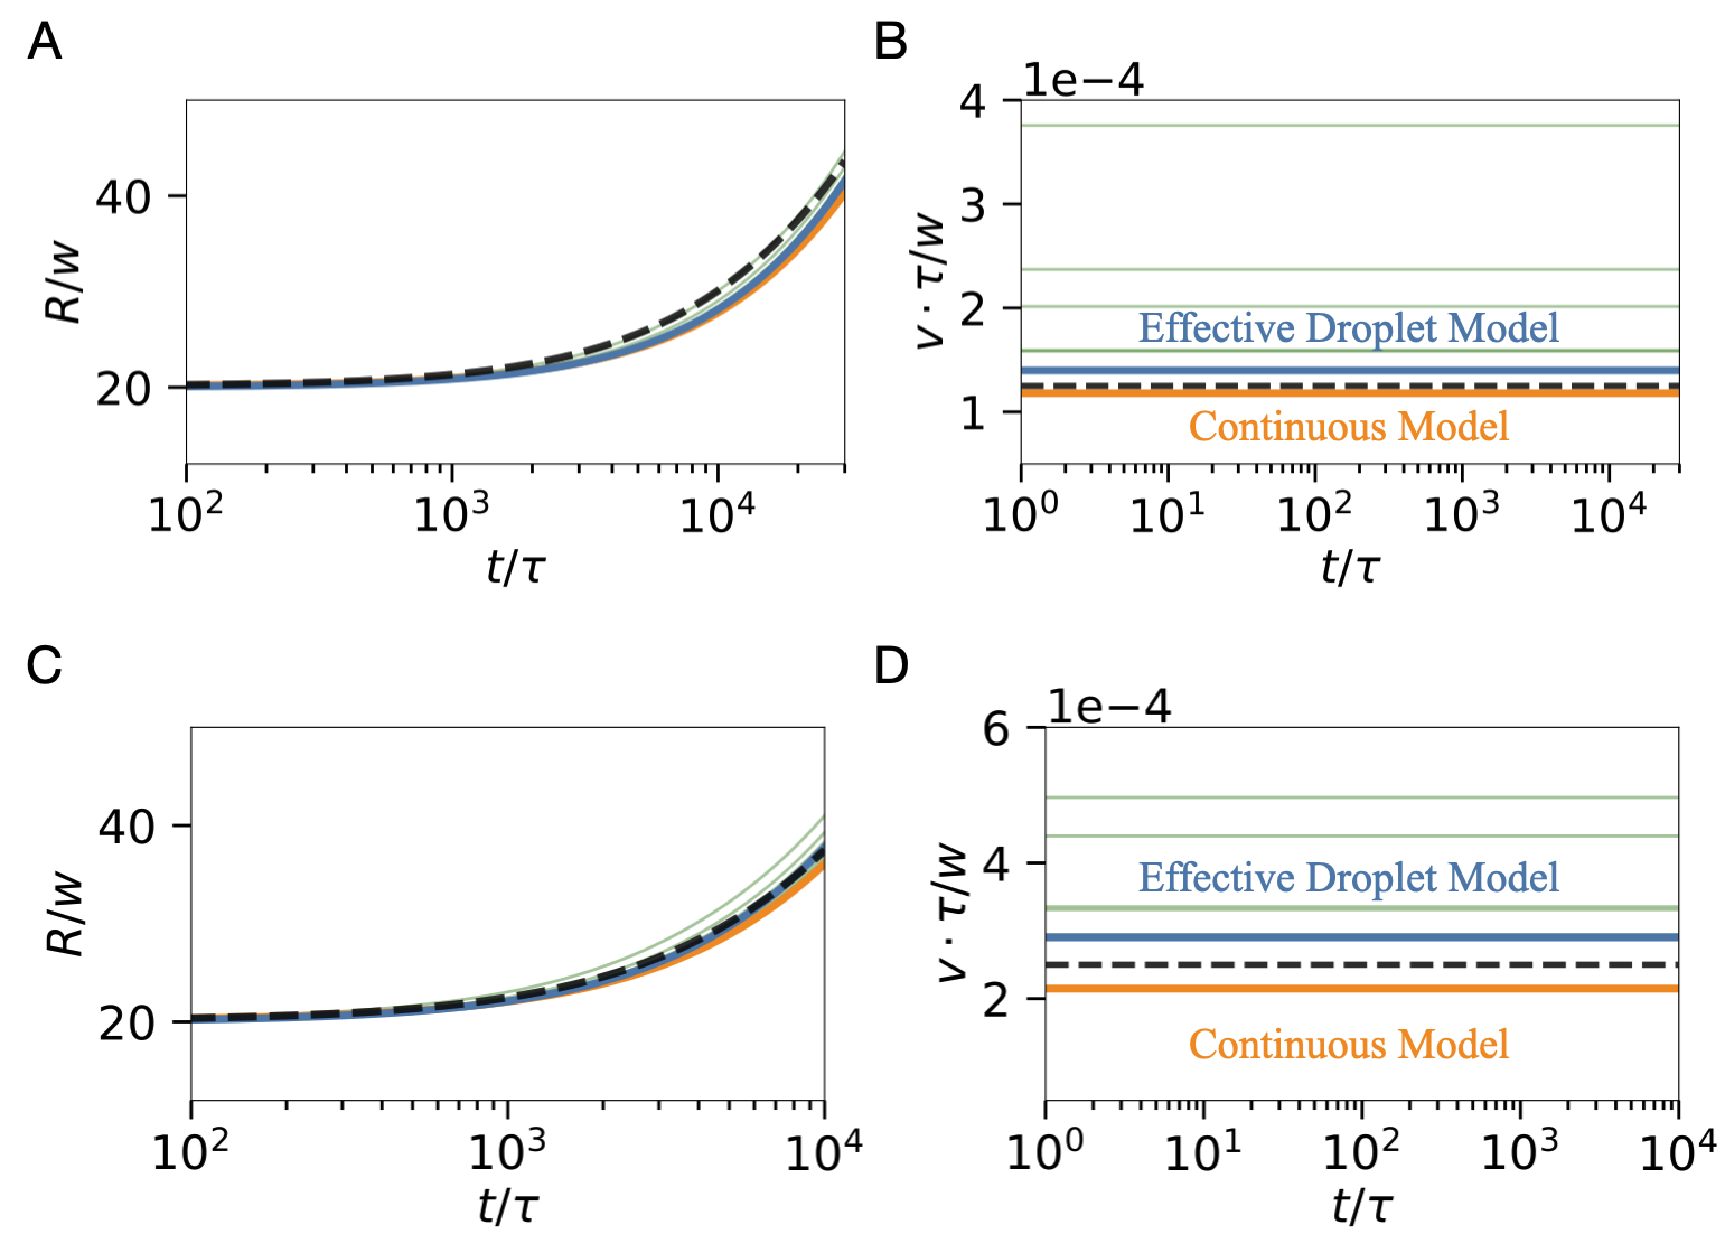
\includegraphics[scale=0.5]{MainContent/Figures/drop_in_gradient_all.pdf}
\caption{
\textbf{Effect of varying shell thickness $\ell$ on droplet dynamics in external gradients.}
(A, C) show droplet radius $R$ and (B, D) show drift speed $v$ as a function of time $t$ for continuous model (orange), the effective droplet model with optimum parameters $(\dx \approx \ell \approx \ds \approx R_0)$ (blue), the effective droplet model with varying shell thickness $\ell$ (green) and the analytical prediction (dashed line).
\mbox{(A, B)} Simulations performed for the same parameters as in \figref{fig:drop_in_gradient}A and \figref{fig:drop_in_gradient}B.
\mbox{(C, D)} Simulations performed for the same parameters as in \figref{fig:drop_in_gradient}C and \figref{fig:drop_in_gradient}D.
Droplet growth remains fairly unaffected, but droplet drift speed $v$ is highly sensitive to changes in $\ell$, with (B) and (D) highlighting the importance of choosing the optimum value for $\ell$.
Shell thickness values are uniformly chosen between $\ell \in [0.25 R_0, 10R_0]$ with $\dx \approx \ds \approx R_0$.
}
\label{fig:drop_in_gradient_all}
\end{figure}

Lastly, we study the accuracy of the effective droplet model for simulation parameters other than the optimum values.
We keep $\dx, \ds$ at their optimum value ($\dx \approx \ds \approx R_0$), but uniformly vary the shell thickness between $\ell \in [0.25 R_0, 10R_0]$.

Fig. \ref{fig:drop_in_gradient_all} reveals the importance of choosing the optimum value for $\ell$ and further validates our choice of the optimum simulation parameters.
For both the cases - high (Fig. \ref{fig:drop_in_gradient_all}A, Fig. \ref{fig:drop_in_gradient_all}B) and low (Fig. \ref{fig:drop_in_gradient_all}C, Fig. \ref{fig:drop_in_gradient_all}D) strength of the gradient $\beta$, the droplet growth remains unaffected but the drift speed $v$ is highly sensitive to the value of $\ell$.
Strong deviations from the droplet drift speed occur for values of $\ell$ which are either too small or too large compared to $\dx$.
As mentioned before, the flux $\jOut^{(m)} \cdot \vec{n}$ outside each droplet for each $m$-th shell sector scales with $\ell^{-1}$; see Appendix \ref{sec:fluxes_inside_shell}.
Thus small values of $\ell$ imply larger fluxes, implying a stronger droplet drift speed. 
For values of $\ell$ which are too large, the droplet drift speed again deviates strongly from the analytical prediction from \Eqsref{eqn:thin_interface_model}.
This is because for large $\ell$, the value of $\phiShell^{(m)}$ is higher than the true value (which is near the droplet) as a result of the gradient of $\phiOut$.
Thus, for large $\ell$, $\phiShell^{m}$ is calculated far away from the droplet, leading to an erroneous representation of $\phiOut$ close to the droplet.
Lastly, we also perform simulations for 2 dimensional systems; see Appendix \ref{sec:droplet_gradient_2D}, and validate our choice for the optimum simulation parameters. 

Taken together, the effective droplet model accurately captures the effects of external gradients on droplet dynamics, both in low and high values of the gradient and for two; see Appendix \ref{sec:droplet_gradient_2D}, and three dimensional systems. 
However, the difference in simulation times is stark between the continuous model ($\sim 10 \mathrm{~simulation~days}$) and the effective droplet model ($\sim 10 \mathrm{~simulation~minutes}$ with optimum parameters) with identical High-performance computing hardware for simulations in \figref{fig:drop_in_gradient} and \figref{fig:drop_in_gradient_all}, thus making the effective droplet model a computationally viable alternative to the continuous model when simulating such systems.

Next, we shift our attention to demonstrating the hallmark of this model - which is the ability to simulate large three dimensional systems with many droplets.
Note that again we do not simulate this scenario using the continuous model, as it is computationally expensive.
In this case, we compare the effective droplet model only with analytical predictions. 
We begin by discussing the interactions of many passive droplets in a dilute emulsion.

\section{\textit{Ostwald-Ripening} in passive emulsions}

In emulsions consisting of many passive droplets, large droplets typically grow at the expense of smaller droplets, a phenomenon known as \textit{Ostwald-Ripening}; see Refs. \cite{Review2019,LSWanalytics}.
Consider a system of $N$ passive droplets with radii $R_i$, which are far apart from each other. 
The droplets are immersed in a large background field of low supersaturation and hence, nucleation events are rare.
As the droplet density is small and the supersaturation is low, all the droplets share a common supersaturation $\phi_\infty (t)$, through which all droplet-droplet interactions are mediated.
Each droplet then behaves like an isolated droplet which experiences a volume fraction $\phi_\infty(t)$ far away from it, which depends on the number of droplets present and on time.
From volume conservation, the dynamics of the supersaturation $\phi_\infty$ is described as:
\begin{equation}
\label{eqn:LSW_theory}
    \overline{\phi}\,V_\mathrm{system} = \phiEqIn \, \sum_{i=1}^{N} V_i(t) + \phi_\infty(t) \left ( V_\mathrm{system} - \sum_{i=1}^{N} V_i(t) \right ),
\end{equation}
where $V_\mathrm{system}$ is the system volume, $V_i(t)$ is the volume of a single droplet of radius $R_i(t)$.
Thus, droplet dynamics is still determined by \Eqref{eqn:interfacefluxes_passive}, but the supersaturation each droplet encounters far from it is governed by \Eqref{eqn:LSW_theory}.

Assuming a large system as compared to the droplet volumes $V_\mathrm{system} \gg \sum_{i=1}^{N} V_i(t)$ and neglecting any spatial correlations between the droplets, Lifshitz and Slyozov predicted that the average droplet radius $\left \langle R_i \right \rangle$ grows as $t^{1/3}$ in this case; see Refs. \cite{Lifshitz,Wagner,LSWanalytics}.
In such dilute emulsions, large droplets grow at the expense of smaller droplets, in which the average droplet radius $\left \langle R \right \rangle$ in the system grows as $\left [ {\left \langle R_i \right \rangle} ^{3}(t) - {\left \langle R_i \right \rangle}_0^{3}(t) \right ] \propto t$, where ${\left \langle R_i \right \rangle}_0$ indicates the initial average radius of the droplets.

Furthermore, in the limit of vanishing supersaturation, \textit{Ostwald-Ripening} follows the \textit{Lifshitz-Slyozov-Wagner} scaling laws, where the re-scaled radius $\rho = R_i/{\left \langle R_i \right \rangle}$ follows a universal shape of the droplet-size distribution $H(\rho)$; see Refs. \cite{Review2019,LSWanalytics}, as:

\begin{equation}
\label{eqn:LSW_histogram}
    H(\rho) = \frac{4}{9} \, \rho^2\left ( 1+ \frac{\rho}{3} \right ) ^ {-7/3} \left ( 1-\frac{2 \rho}{3} \right )^{-11/3} \mathrm{exp} \left ( 1 - \frac{3}{3 - 2\rho} \right ).
\end{equation}
Having briefly described the analytical predictions for droplet growth and size distribution for a system of passive droplets undergoing \textit{Ostwald-Ripening}, we next demonstrate that our effective droplet model captures these predictions well. 

Indeed our simulation of $10^5$ droplets indeed recovers the $t^{1/3}$ scaling; see \figref{fig:passive_emulsions}A, when we simulate a dilute emulsion by setting the discretization $\dx$ to the system size (and thus $\ell \approx \dx$), as a mean-field approach is desired.
Note that we need a single sector to discretize the vicinity of each droplets, as they are assumed to be far from each other and thus their vicinity is nearly isotropic.
Moreover, \figref{fig:passive_emulsions}B shows that the distribution of radii also follows the universal shape $H(\rho)$ given by \Eqref{eqn:LSW_histogram}.
Our effective model thus faithfully captures the dynamics of many droplets, optionally even beyond the Lifshitz-Slyozov regime by increasing the spatial resolution to capture correlations in droplet growth.

\begin{figure}[tb]
\centering
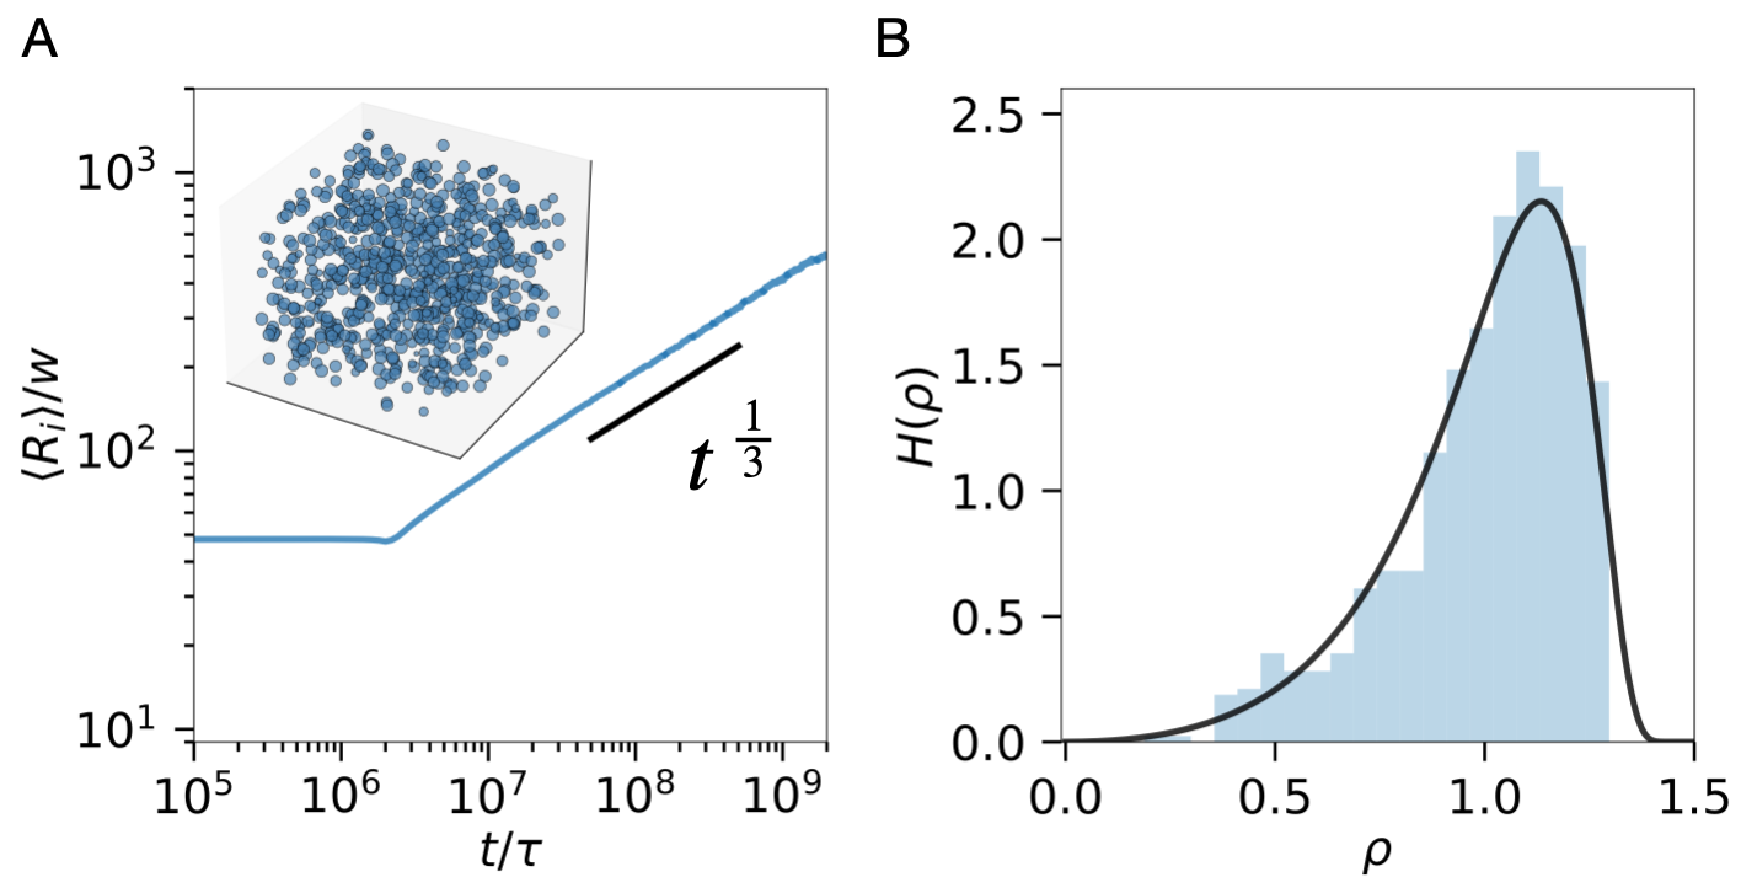
\includegraphics[scale=0.5]{MainContent/Figures/passive_emulsions.pdf}
\caption{\textbf{\textit{Ostwald-Ripening} in passive emulsions}.
(A) Mean droplet radius $\langle R_i \rangle$ as a function of time $t$ shows the expected scaling $\langle R_i \rangle \propto t^{1/3}$; see Refs. \cite{Lifshitz,Wagner,LSWanalytics}.
Inset shows snapshot at $t=2 \times 10^8 \tau$.
(B) Frequency $H(\rho)$ of the re-scaled mean radius $\rho = R_i/\left \langle R_i \right \rangle$ at $t = 2 \times 10^8 \tau$ compared to the expected universal distribution (black); see Refs. \cite{Lifshitz,Wagner}.
(A, B)
Simulations using the effective droplet model were carried out in a $3$ dimensional periodic cubic domain of size $[0, L]^3$, where $L = 10^4 w$.
We used $\Delta x \approx \ell \approx L$ and a single shell sector to approach the mean field solution.
$10^5$ droplets were initialized with radii chosen uniformly in $[9.5 w, 10.5 w]$ in an initial background field $\phiOut(t=0) = 0.05$.
Remaining parameters are specified in Fig. \ref{fig:droplet_pair_schematics}.
}
\label{fig:passive_emulsions}
\end{figure}

\subsection{Effect of simulation parameters}

Next, we briefly look at the effect of the simulation parameter time-step $\dt$ on the coarsening dynamics of passive droplets in a dilute emulsion.
The time-step is a crucial simulation parameter, as it plays an important role in capturing the dynamics of the droplets given by \Eqsref{eqn:DropletDiscretized}.
\figref{fig:passive_emulsions_all} shows the effects of choosing time-steps which are higher than the optimum time-step $\dt_\mathrm{optimum}$ dictated by \Eqref{eqn:time_step}.

As expected, higher values of $\dt$ lead to an incorrect capturing of the $t^{1/3}$ scaling of the average droplet radius $\left \langle R_i \right \rangle$, as seen from \figref{fig:passive_emulsions_all}.
This is because in the mean-field limit with no chemical reactions, the smallest time-step is $\dt_\mathrm{droplets} = 0.1 \mean{R_i}^2/D_\mathrm{out}$ (as $\dx \approx \ell \approx L$, where $L$ is the system size), which also dictates the final time-step given by \Eqref{eqn:time_step}.
Thus choosing a time-step $\dt$ which strays away increasingly from $\dt_\mathrm{optimum}$ given by \Eqref{eqn:time_step} will naturally lead to incorrect capturing of the diffusive fluxes between the droplets, leading to an incorrect scaling for the droplet radii. 
Thus, our choice of the time-step $\dt$ from \Eqref{eqn:time_step} is indeed an optimum choice as seen from \figref{fig:passive_emulsions_all}.

\begin{figure}[tb]
\centering
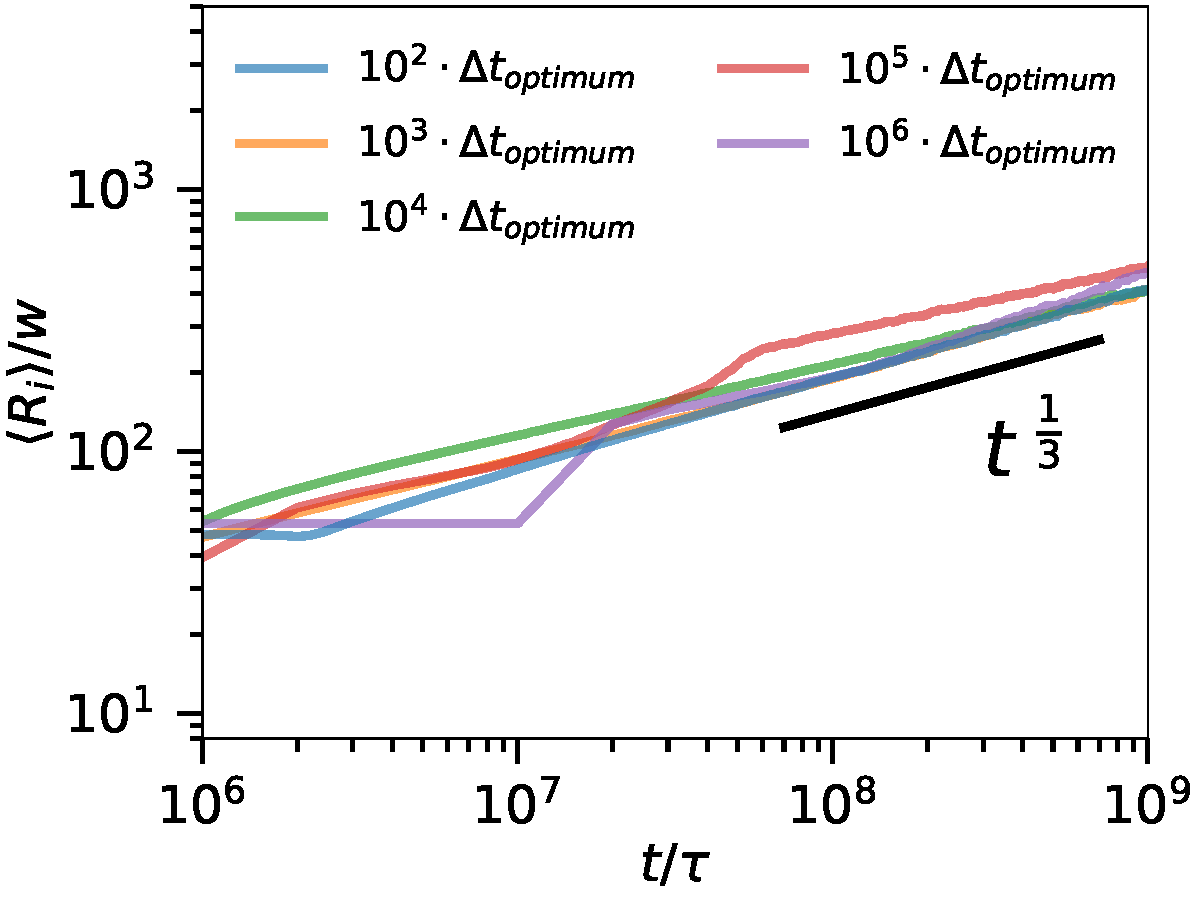
\includegraphics[scale=0.5]{MainContent/Figures/LSW_all.pdf}
\caption{\textbf{Effect of time-step $\dt$ on \textit{Ostwald-Ripening} in passive emulsions}.
Mean droplet radius $\langle R_i \rangle$ as a function of time $t$ shows the expected scaling $\langle R_i \rangle \propto t^{\,1/3}$; see Refs. \cite{Lifshitz,Wagner,LSWanalytics}, for low values of time-step $\dt$ and deviates strongly for higher $\dt$, thus validating our choice of the optimum time-step $\dt$ obtained from \Eqref{eqn:time_step}.
Remaining parameters are specified in Fig. \ref{fig:passive_emulsions}.
}
\label{fig:passive_emulsions_all}
\end{figure}

\section{Suppression of \textit{Ostwald-Ripening} in active emulsions}

As a final example for demonstrating the effective droplet model, we consider the interaction of many active droplets in a dilute emulsion.
In the case of simple first order reactions which convert droplet material $A$ into background field material $B$, \textit{Ostwald-Ripening} is suppressed and multiple droplets of a fixed size are produced; see Ref. \cite{Zwicker2015}.

% Such reactions are also present in biology, where $A,B$ can represent two states of a protein with their conversion facilitated by phosphorylation dephosphorylation reactions when the energy source is adenosine triphosphate molecules; see Ref. \cite{AlbertsBook2003}.
% Thus, simple reactions like these can be thought of as useful toy models and can provide insights into how the cell manages to regulate and finely tune the size of the condensates.

Generally speaking, in the case of first order reactions, we can argue towards the existence of a stable size for the droplets through balance between material fluxes inside and outside the droplet as follows:
droplet material is produced mainly in the background field and diffuses toward the droplet.
Inside the droplet, it gets destroyed due to chemical reactions which convert droplet material into background field material; which then diffuses into the background field.

As will be shown later, the total material flux inside the droplet $\vec{J}_\mathrm{in}$ scales as droplet volume, whereas the total material flux outside the droplet $\vec{J}_\mathrm{out}$ scales with the droplet radius.
Hence, we qualitatively expect the droplet to have a stable size based on the balances of the fluxes.
We elaborate on this point in the next section, where we study the effects of first order reactions on a single isolated droplet. 
Note that although the effective droplet model is formulated for generic reactions with complicated expressions for the reaction fluxes $s(\phiIn), s(\phiOut)$, here we focus on demonstrating the model for simple first-order reactions with linearized reaction fluxes which depend only on the composition.

We utilize a thin-interface description approach to formulate the dynamics of the volume fraction inside ($\phiIn$) and outside ($\phiOut$) the droplets; see Refs. \cite{Zwicker2015,Review2019}.
The chemical reaction scheme for the first-order reactions looks as:
\begin{equation}
\label{eqn:reaction_scheme}
    A \underset{\kf}{\stackrel{\kb}{\rightleftharpoons}} B,
\end{equation}
where droplet material A gets converted into background field material B inside the droplet with the rate $\kb$ and the background field material gets converted into droplet material inside the background field with the rate $\kf$.
Hence, the reaction flux in \Eqref{eqn:reaction_scheme} for both: inside the droplet and outside the droplet (i.e. inside the background field) reads as $s(\phi_\mathrm{in/out}) = \kf (1 - \phi_\mathrm{in/out}) - \kb \, \phi_\mathrm{in/out}$.
As we are interested in regimes where droplets are stable, we assume that local thermal equilibrium is quickly established and limit ourselves to regimes where $\kf, \kb$ are small as compared to the rate obtained from diffusion across the interface of the droplets given by $D_\mathrm{(in/out)} / w^2$; see Ref. \cite{Zwicker2015}.

First, we focus on the simple case of a single active droplet achieving a stable size, and then shift our attention to systems with multiple active droplets which exhibit suppression of \textit{Ostwald-Ripening}.

\subsection{Single active droplet in a large background field}
As mentioned before, active droplets can achieve a stable radius based on the balance of fluxes across the interface.
We aim to derive this stable radius for an active droplet with first-order chemical reactions immersed in a large background field, using the thin-interface approximation for the droplets; see Refs. \cite{Zwicker2015,Review2019}.

Similar to the case of a passive droplet in a large background field, we again assume strong phase separation and assume that $\phiIn,~\phiOut$ themselves vary little inside the droplet and the background field respectively.
Typically in a large system, chemical equilibrium is achieved far from the droplet when the reaction flux $s(\phi)=0$ and the average volume fraction is given by $\phi_\infty = \kf/(\kf + \kb)$; see Refs. \cite{Zwicker2015,Review2019}.

Consider an isolated active droplet of radius $R \gg w$ immersed in a large background field.
Owing to symmetry, we place a spherically symmetric co-ordinate system at the centre of the droplet with $r$ being the radial co-ordinate.
Since $\phiIn$ typically varies only a little, we use the thin-interface approximation; see \Eqsref{eqn:thin_interface_model}, of the continuous model to approximately arrive at the dynamical equation for $\phiIn$ as:

\begin{align} 
    \label{eqn:RD_droplet_firstorder}
    \frac{\partial \phiIn}{\partial t}
        \approx D_\mathrm{in} \nabla^2 \phiIn +
         \kf (1 - \phiIn) - \kb (\phiIn),
\end{align}
where $D_\mathrm{in}$ is the diffusivity inside the droplet.
We can analytically solve for $\phiIn$ from the stationary state of \Eqref{eqn:RD_droplet_firstorder}, using the boundary conditions $\phiIn(R) = \phiEqIn$ and $\partial_r \phiIn (0) = 0$ and obtain 
\begin{equation*}
    \phiIn(r) = \left (\phiEqIn - \phi_\infty \right ) \left( \frac{R}{r} \right ) \frac{\sinh \left(\frac{r}{\xi_\mathrm{in} }\right)}{\sinh \left(\frac{R}{\xi_\mathrm{in} }\right)} + \phi_\infty.
\end{equation*}

The solution reveals that $\phiIn$ increases monotonically inside the droplet till it attains a value $\phiEqIn$ and varies on the characteristic reaction-diffusion length-scale $\xi_\mathrm{in}=\sqrt{D_\mathrm{in}/({\kf + \kb})}$; see Ref. \cite{Review2019}.

Similar to inside the droplet, the volume fraction in the background field $\phiOut$ also typically varies a little and is hence described from the thin-interface approximation; see \Eqsref{eqn:thin_interface_model}, as:

\begin{align} 
    \label{eqn:RD_dilute_firstorder}
    \frac{\partial \phiOut}{\partial t}
        \approx D_\mathrm{out} \nabla^2 \phiOut +
         \kf (1 - \phiOut) - \kb \phiOut,
\end{align}
where $D_\mathrm{out}$ is the diffusivity outside the droplet.
Outside the droplet, we solve for $\phiOut$ from the stationary state of \Eqref{eqn:RD_dilute_firstorder}, using the boundary conditions $\phi_\mathrm{out}(R) = \phiEq_\mathrm{out}$ and $\phiOut(\infty) = \phi_\infty$.
We thus obtain 
\begin{equation*}
    \phiOut(r) =  [\phiEqOut - \phi_\infty] \left [ \frac{R}{r} \right ] e^{\left({\frac{R - r}{\xi_\mathrm{out}}}\right)} + \phi_\infty.
\end{equation*}
This solution also reveals that $\phiOut$ increases/decreases monotonically from $\phiEqOut$ to $\phi_\infty$ and varies on the characteristic reaction-diffusion length-scale, $\xi_\mathrm{out}=\sqrt{D_\mathrm{out}/({\kf + \kb})}$.
Simply put, $\phiOut$ reaches a value $\phi_\infty$ at a distance of roughly $\xi_\mathrm{out}$ from the droplet surface.
Thus, when we mean large systems, we consider system sizes $L$ which are $L \gg \xi_\mathrm{out}$, which is the definition we use in this thesis.
Consequently, finite systems would imply $L \sim \xi_\mathrm{out}$.

Spatial gradients in $\phiIn$ and $\phiOut$ at the droplet surface lead to local material fluxes outside the droplet as $\vec{j}_\mathrm{out} = [-D_\mathrm{out} {\boldsymbol{\nabla}} \phiOut (R)]$ and inside the droplet as $\vec{j}_\mathrm{in}  = [-D_\mathrm{in} {\boldsymbol{\nabla}} \phiIn (R)]$.
Note that, we typically assume same diffusivity $D$ inside and outside the droplets, i.e. $D_\mathrm{out} \approx D_\mathrm{in} = D$, which also implies $\xi_\mathrm{in} \approx \xi_\mathrm{out} = \xi$.
The fluxes then read as:
\begin{subequations}
\label{eqn:fluxes_in_firstorder}
\begin{align}
    \jIn \cdot \vec{n} &= D (\phiEqIn  - \phi_\infty) \left[ \frac{1}{R} - \frac{\coth \left (\frac{R}{\xi}\right )}{\xi} \right ] \mathrm{~and~}
    \\[10pt]
   \jOut \cdot \vec{n} &= 
    D (\phiEqOut  - \phi_\infty) \left[ \frac{1}{R} + \frac{1}{\xi} \right ].
\end{align}
\end{subequations}
We can now calculate the interfacial speed $v_n$ from \Eqref{eqn:InterfacialSpeed} and thus arrive at the stationary states for the droplet by numerically solving for $v_n = 0$.
This typically reveals two solutions $R_\ast, \overline{R}$ (as $\phiEqIn,~\phiEqOut$ depend on the droplet radius $R$; see \Eqsref{eqn:GibbsThompsonRelations}).

Droplets smaller than the critical radius $R_{\ast}$, defined as the radius at which the equilibrium volume fraction of the droplet equals the local supersaturation, dissolve quickly and is hence an unstable radius. 
On the other hand, droplets greater than $R > R_{\ast}$ grow until they reach the radius $\overline{R}$ and don't grow any further.
This follows from \Eqsref{eqn:fluxes_in_firstorder} as: For $R \ll \xi$, $\vec{J}_\mathrm{in} = \int_\Omega \jIn~\mathrm{d}A = 4 \pi R^2 \,\jIn$ scales with the volume of the droplet, which is seen from expanding the last term in $\jIn\cdot \vec{n}$ as $\left [\xi - R \coth \left (\frac{R}{\xi}\right ) \right ] \Big {/} (R \, \xi) \approx -R/(3\,\xi^2)$.
On the other hand, $\vec{J}_\mathrm{out} = \int_\Omega \jOut~\mathrm{d}A = 4 \pi R^2 \,\jOut$ scales with the radius of the droplet, which is seen from expanding the last term in $\jOut\cdot \vec{n}$.
Hence destruction of droplet material due to $\vec{J}_\mathrm{in}$ takes over if the droplet starts to grow bigger than $\overline{R}$.
The droplet then shrinks back to $\overline{R}$, thus indicating that this is the stable radius. 

Having numerically solved for the stable radius $\overline{R}$ after equating the fluxes from \Eqsref{eqn:fluxes_in_firstorder} for large systems, we now show that our effective droplet model agrees well with these predictions.
Indeed, as seen from Fig. \ref{fig:active_droplet_3D}A, the stable radius $\overline{R}_\mathrm{3D}$ (black line) obtained from the analytics ($\jIn = \jOut$ in \Eqsref{eqn:fluxes_in_firstorder}) compares well with simulations of the effective droplet model with optimum parameters (blue line) for large systems, but deviates from the continuous model (orange line).
This deviation occurs because $\overline{R}_\mathrm{3D}$ is a numerical solution from setting $\jIn = \jOut$ in \Eqsref{eqn:fluxes_in_firstorder}.
We simulate the effective droplet model for a single active droplet of initial radius $R_0 = 4w$ in a periodic 3 dimensional large system of size $[0, L_1]^3$, where $L_1 = 767w$.
We start with an initial background field $\phiOut(t=0) = \phi_\infty$, and the droplet grows until it reaches a stable radius.
Simulations using the continuous model were carried out for a droplet of initial radius $R_0 = 4w$ with $\phi(t=0) = \phi_\infty$ in a spherically symmetric domain of size $r \in [0, 5 \xi]$.
We choose optimum parameters, which in this case are $\dx \approx \ell \approx \ds \approx R_0$, as we desire to accurately model the vicinity of the droplet and the resulting fluxes.

\begin{figure}[tb]
\centering
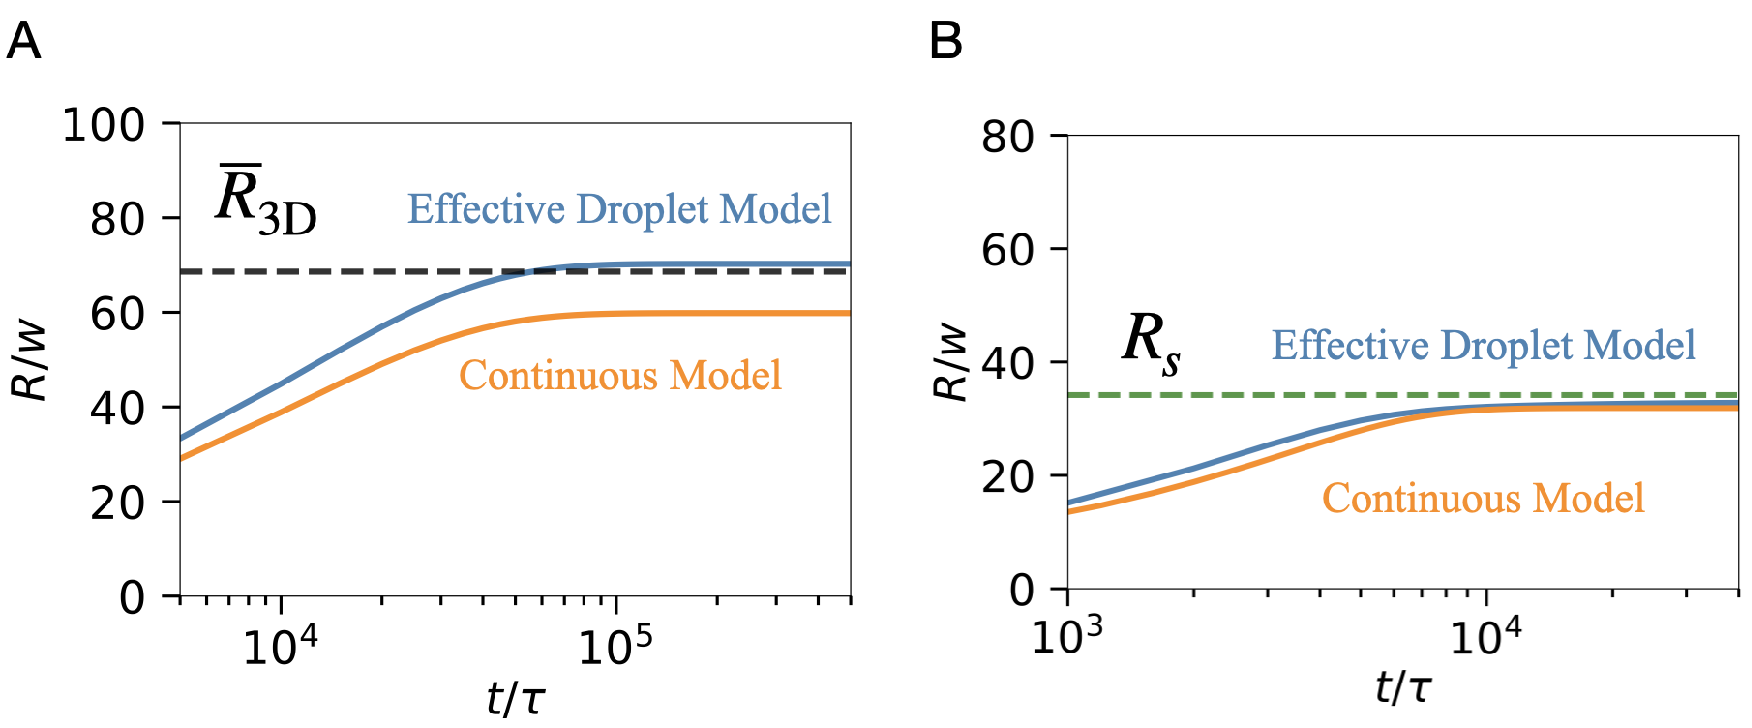
\includegraphics[scale=0.5]{MainContent/Figures/active_droplet_3D.pdf}
\caption{\textbf{Single active droplet reaches a stable radius in a large system (A) and a finite system (B).}
(A) Droplet radius $R$ as a function of time $t$.
The droplet reaches a fixed size $\overline{R}_\mathrm{3D}$ (dashed line) in a large system. 
$\overline{R}_\mathrm{3D}$ is obtained from numerically solving for $\jIn = \jOut$ from \Eqsref{eqn:fluxes_in_firstorder}, compares well with the effective droplet model (blue) and deviates from the continuous model (orange).
Simulations using the effective droplet model were carried out for a droplet of initial radius $R_0 = 4 w$ with $\phiOut(t=0) =\phi_\infty$ in a $3$-dimensional periodic cubic domain of size $[0, L_1]^3$, where $L_1 = 767w$ with $\dx \approx \ell \approx \ds \approx R_0$.
Simulations using the continuous model were carried out for a droplet of initial radius $R_0 = 4 w$ with $\phi(t=0) = \phi_\infty$ in a spherically symmetric domain of size $r \in [0, 5 \xi]$.
(B) Droplet reaches a fixed radius $R_s$ (dashed green line) given by \Eqref{eqn:approx_stable_radius_finite} for a finite system and compares well with simulations using the effective droplet model (blue) and using the continuous model (orange).
% Inset shows the volume fraction $\phi$ as a function of the radial co-ordinate $r$ from simulations of the continuous model at time $t = 4 \times 10^4 \tau$, with stable droplet radius $R_s$ (dashed green line) and $\phi = \phi_\infty$ (dashed black line).
% Far from the droplet, $\phi$ reaches a value which significantly lower than $\phi_\infty$, as is expected for a finite system.
Simulations using the continuous model were carried out for a droplet of initial radius $R_0 = 4 w$ with $\phi(t=0) =\phi_\infty$ in a spherically symmetric domain of size $r \in [0, 0.8 \xi]$.
Simulations using the effective droplet model were carried out with $\phiOut(t=0) = \phi_\infty$ in a $3$-dimensional periodic cubic domain of size $[0, L_2]^3$, where $L_2 = 122w$.
As $R_s$ is calculated from a mean-field approach, simulation parameters were $\dx \approx \ell \approx \ds \approx L_2$.
\mbox{(A-B)}
Model parameters are $s(\phi)= \kf (1 - \phi) - \kb \phi$, $\kf = 1 \times 10^{-5} \tau^{-1}$ and $\kb = 1 \times 10^{-4}  \tau^{-1}$.
Remaining parameters are specified in Fig. \ref{fig:droplet_pair_schematics}.
}
\label{fig:active_droplet_3D}
\end{figure}

We also simulate a single active droplet reaching it's fixed size for a large 2 dimensional system and compare it with the analytical predictions, too study how well the effective droplet model works for two dimensions.
As seen from Fig. \ref{fig:active_droplet_2D_infinite}, the stable radius $\overline{R}_\mathrm{2D}$ obtained from the analytical predictions ($\jIn = \jOut$ in \Eqsref{eqn:fluxes_in_firstorder}) compares well with simulations of the effective droplet model with optimum parameters.
We simulate the effective droplet model for a single active droplet of initial radius $R_0 = 4w$ in a periodic 2 dimensional large system of size $[0, L_1]^3$, where $L_1 = 843w$.
We start with an initial background field $\phiOut(t=0) = \phi_\infty$, and the droplet grows until it reaches a stable radius.
We choose optimum parameters as well, which in this case are $\dx \approx \ell \approx \ds \approx R_0$.
Simulations using the continuous model were carried out for a droplet of initial radius $R_0 = 4w$ with $\phi(t=0) = \phi_\infty$ in a polar domain of size $r \in [0, L_2]$, where $L_2 = 5 \xi$.

Additionally, it is again interesting to see that increasing approximations of the continuous model (in orange) lead to increasingly worse estimates for droplet drift, as the analytical predictions from the thin-interface approximation (dashed line); see \Eqsref{eqn:thin_interface_model}, are approximations of the continuous model, and the effective droplet model (in blue) is an approximation of \Eqsref{eqn:thin_interface_model}.

\begin{figure}[tb]
\centering
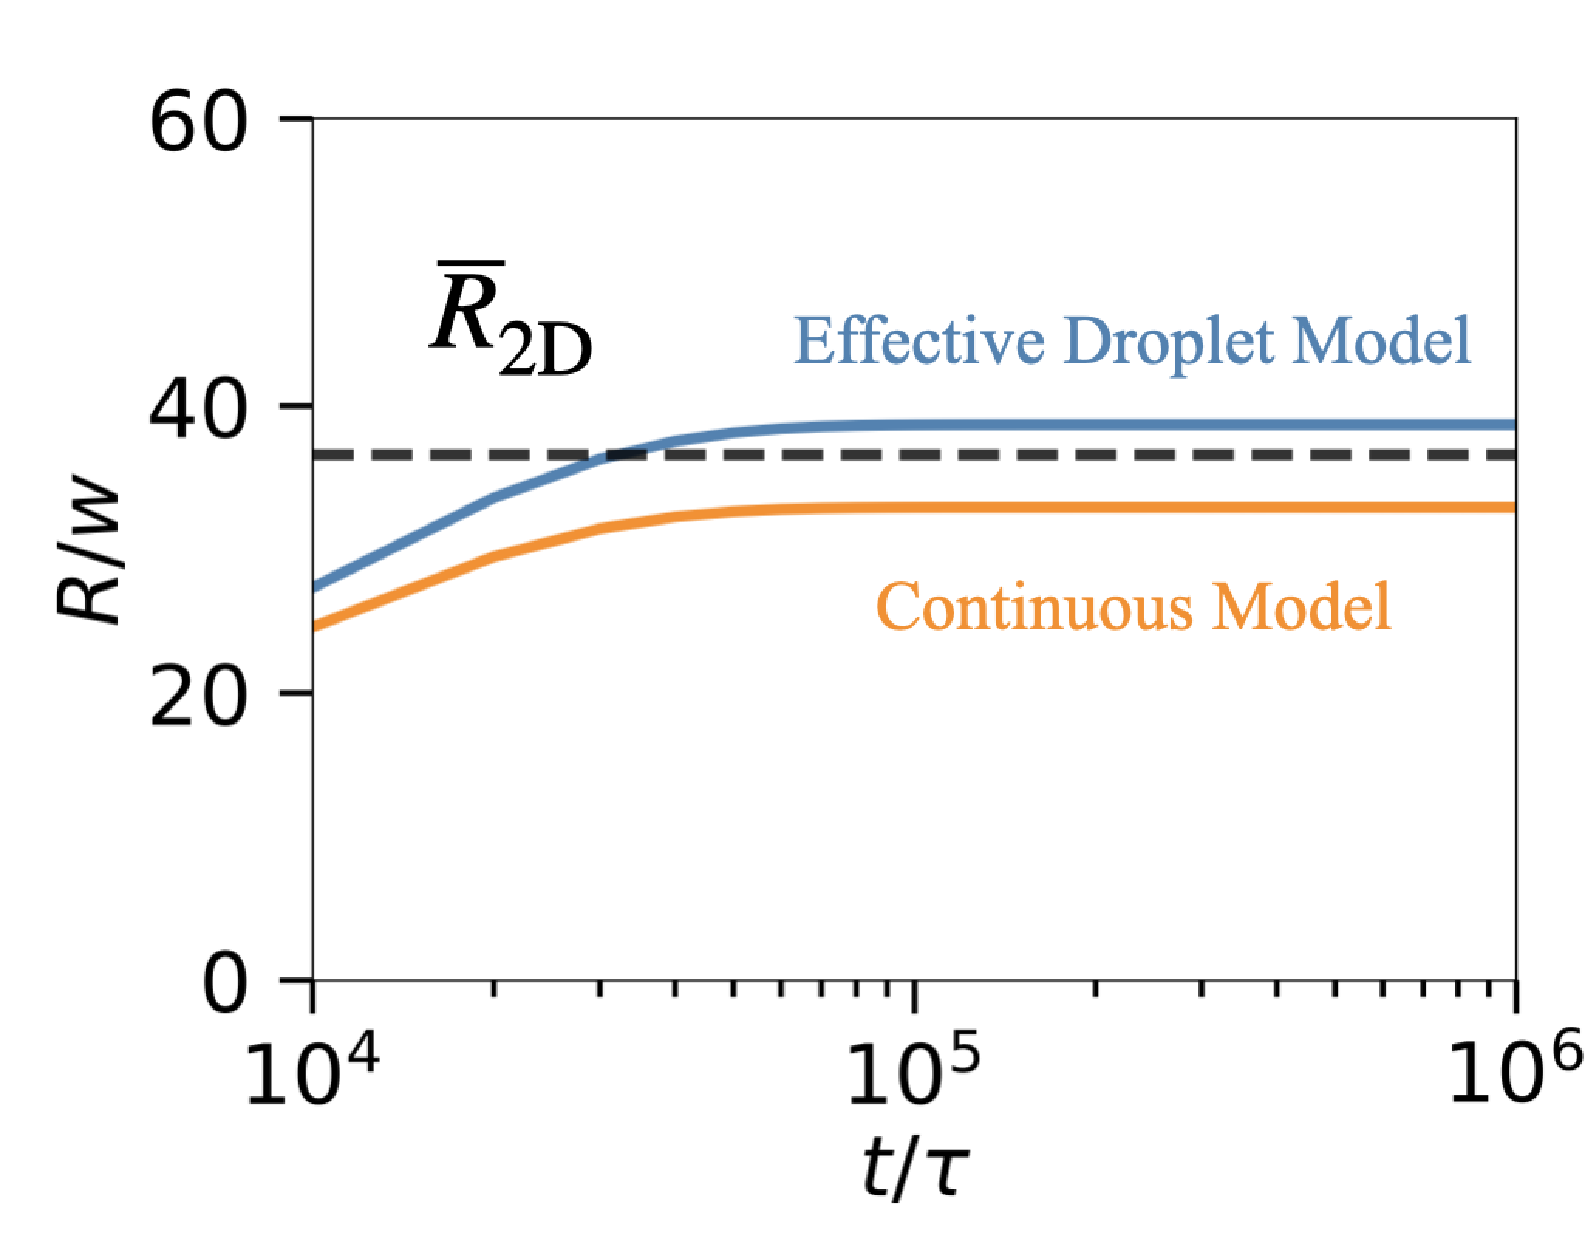
\includegraphics[scale=0.3]{MainContent/Figures/active_droplet_2D_infinite.pdf}
\caption{\textbf{Single active droplet reaches a stable radius in a large two dimensional systems.}
Droplet radius $R$ as a function of time $t$, which reaches a fixed size $R_\mathrm{2D}$ (dashed line) given by numerically solving for $\jIn = \jOut$ from \Eqsref{eqn:fluxes_in_firstorder} for 2 dimensions, and compares well with the effective droplet model (blue) and the continuous model (orange).
Simulations using the effective droplet model were carried out for a droplet of initial radius $R_0 = 4 w$ with $\phiOut(t=0) = \phi_\infty$ in a $2$-dimensional periodic square domain of size $[0, L_1]^2$, where $L_1 = 843 w$.
Simulation parameters were selected as $\dx \approx \ell \approx \ds \approx R_0$.
Simulations using the continuous model were carried out for a droplet of initial radius $R_0 = 4 w$ with $\phi(t=0) = \phi_\infty$ in a polar domain of size $r \in [0, L_2]$, where $L_2 = 5 \xi$.
Model parameters are $s(\phi)= \kf (1 - \phi) - \kb \phi$, $\kf = 1 \times 10^{-5} \tau^{-1}$ and $\kb = 1 \times 10^{-4}  \tau^{-1}$.
Remaining parameters are specified in Fig. \ref{fig:droplet_pair_schematics}.
}
\label{fig:active_droplet_2D_infinite}
\end{figure}

We next consider multiple interacting active droplets and their tendency to suppress \textit{Ostwald-Ripening}, eventually showing that simulations using the effective droplet model recover suppression of \textit{Ostwald-Ripening}.
Note that again we do not simulate this scenario using the continuous model, as it is computationally expensive. 
In this case too, we compare the effective droplet model with analytical predictions. 

\subsection{Multiple interacting active droplets and suppression of \textit{Ostwald-Ripening}}

Until now, we have shown that a single isolated active droplet reaches a stable radius $\overline{R}$ in a large system, which is calculated from a balance of the fluxes $\jIn,~ \jOut$ inside and outside the droplets from \Eqsref{eqn:fluxes_in_firstorder}.
However, a system of active droplets in a finite sized system can also reach a stable radius, effectively suppressing \textit{Ostwald-Ripening}, which amongst other parameters, depends on the reaction rates $\kf, \kb$, the system volume $V_\mathrm{system}$.

In this section, we briefly discuss the mean-field approach developed by Zwicker et al. \cite{Zwicker2015} and elaborate on the stable radius which multiple interacting active droplets in an emulsion attain.
Generally, in an emulsion of $N$ active droplets in a finite sized system, the supersaturation $\overline{\phi}$ in the system which is felt outside each droplet is $\overline{\phi} \leq \phi_\infty$.
This is in contrast to the case of a single active droplet because now the droplet material is limited and has to be shared amongst $N$ droplets.
We thus qualitatively expect the stable radius of the droplets in such a system to be lesser than $\overline{R}$.

The dynamics of $\overline{\phi}$ is governed by the simple reaction-diffusion equation, where we invoke the \textit{quasi-static approximation} and we assume that $\overline{\phi}$ relaxes quickly when compared with the droplet growth rates. 
Taking into account contributions from the droplets following \Eqref{eqn:reaction_scheme}, we arrive at the dynamical equation for $\overline{\phi}$ as:
\begin{equation}
\label{eqn:phi_dynamics}
    \partial_t \overline{\phi} = \kf (1- \overline{\phi}) - \kb (\overline{\phi}) + \frac{\sum_{i=1}^{N}~ \int_{\Omega_{i}} ~ \jIn\cdot \vec{n}}{V_\mathrm{system}},
\end{equation}
where the last term accounts for diffusive fluxes, $\Omega_i$ is the $i^\mathrm{th}$ droplet surface and $V_\mathrm{system}$ is the system volume, along with $V_\mathrm{system} \gg V_\mathrm{total}$. 

Thus, the dynamics of the droplets are still described by the fluxes obtained from  \Eqsref{eqn:fluxes_in_firstorder} and the droplet growth rate from \Eqref{eqn:InterfacialSpeed}, but now the volume fraction far from the droplets is governed by \Eqref{eqn:phi_dynamics}.
We thus arrive at a complete description for the dynamics of $N$ active droplets in a finite system of volume $V_\mathrm{system}$. 

Next, we turn our focus to calculating the fixed radius every droplet in such a system attains.
Consider a system of $N$ active droplets, all of which attain a common radius $R_s$.
The slowest rate of relaxation to such a state is given as:

\begin{equation}
\label{eqn:lambda}
    \lambda = \frac{D w}{6 R_s^3} - \frac{2 \kb}{3},
\end{equation}
which is obtained when a linear stability analysis is performed for \Eqref{eqn:phi_dynamics} and \Eqref{eqn:InterfacialSpeed} around $R_s$; see Refs. \cite{Zwicker2015,Review2019}.
Note that $\lambda$ does not contain any information about the number of droplets, as it considers only a mean-field coupling of the droplet and the background field. 
Furthermore, $\lambda < 0$ implies the steady state $R_s$ is stable, which means that all the droplets have to be greater than the threshold radius given as:
\begin{equation*}
    R_\mathrm{th} = \left [\frac{D w}{4 \kb} \right ] ^ {\frac{1}{3}},
\end{equation*}
obtained by setting $\lambda = 0$.
Thus, multiple droplets can have a stable size only if $R_s > R_\mathrm{th}$. 
In most cases, this condition is satisfied for sufficiently large $\kb$; see Ref. \cite{Zwicker2015}.

Hence, the value of $R_s$ all the $N$ droplets attain depends on the droplet density:
\begin{enumerate}
    \item If the droplet density is small, i.e. $N / V_\mathrm{system} \gg \xi ^ {-3}$, droplets do not significantly alter the volume fraction far from them $(\overline{\phi} \approx \phi_\infty)$; see \Eqref{eqn:phi_dynamics}, and thus the stable radius stays the same for a single active droplet in a large system, i.e. $R_s \approx \overline{R}$.
    Simply put, this means \textit{Ostwald-Ripening} is suppressed in such low density systems and each droplets attains a radius $R_s \approx \overline{R}$.

    \item If the droplet density is large, i.e. $N / V_\mathrm{system} \ll \xi ^ {-3}$, the stable radius $R_s$ is less than $\overline{R}$. 
    This is simply because the total amount of droplet material is limited, which is shared commonly between $N$ droplets.
    In principle, this supersaturation $\overline{\phi}$ is solved from the coupled equations \Eqref{eqn:phi_dynamics} and \Eqref{eqn:InterfacialSpeed}.
    However, we can approximately calculate $\overline{\phi}$ by arguing that the total volume of droplet material $V_\mathrm{system}~\phi_\infty$ is an upper bound for the total droplet volume, i.e. $N \, V_s \approx V_\mathrm{system} \, \phi_\infty$.
    The stable radius $R_s$ can then be simply calculated as:
    \begin{equation}
    \label{eqn:approx_stable_radius_finite}
        R_s = \left [\frac{3 V_s}{4 \pi}\right ]^{\frac{1}{3}},
    \end{equation}
    and thus \textit{Ostwald-Ripening} is again suppressed, but with droplets of a smaller size than $\overline{R}$.

\end{enumerate}
We can also qualitatively explain why does a system of $N$ active droplets with first-order reactions attain a state where all the droplets have the same radius given by $R_s$.
In the absence of chemical reactions, \textit{Ostwald-Ripening} is observed and droplets coarsen over time, which is also seen from \Eqref{eqn:lambda} - when chemical reactions are absent, $\lambda > 0$ and is proportional to the size of the droplets.
The primary reason for small droplets to shrink and big droplets to grow bigger is surface tension, as the material flux is directed from the smaller droplets (having a high value of $\phiEqOut$) towards the bigger droplets (having a low value of $\phiEqOut$).
However, in the case of first order reactions, surface tension effects will be countered by diffusive fluxes originating from the background field into the droplet due to chemical reactions and hence multiple droplets of the same size can co-exist.

Having developed a mean-field framework for calculating the fixed size for a system of $N$ active droplets, we aim to demonstrate that the effective droplet model is able to capture this fixed size which the droplets attain.
We choose three different mean-field coarsening scenarios in increasing complexity and compare simulations using the effective droplet model with the analytical predictions:

\begin{enumerate}
    \item A single active droplet in a finite system.
    
    \item A pair of active droplets coarsening in a large and a finite system.

    \item Multiple active droplets coarsening in a large and a finite system.
    \end{enumerate}

%%%%%%%%%%%%%%%%%%%%%%%%%%%%%%%%%%%%%%%%%%%%%%%%%%%%%%%%%%%%%%%%%%%%%%%%

\subsubsection{Coarsening of a single active droplet in a finite system}

We start by demonstrating that the effective droplet model captures the mean-field coarsening of a single active droplet in a finite system.
We simulate a droplet of initial radius $R_0 = 4 w$ embedded in an initial volume fraction $\phi_\infty = \kf/(\kf + \kb)$ and let it coarsen over time.
As seen from Fig. \ref{fig:active_droplet_3D}B, the droplet reaches a fixed radius $R_s$ (dashed green line) given by \Eqref{eqn:approx_stable_radius_finite} and compares well with simulations using the effective droplet model (blue) and using the continuous model (orange).
% Inset of Fig. \ref{fig:active_droplet_3D}B shows the volume fraction far from the droplet reaches $\phi \ll \phi_\infty$, as we correctly assumed.
Note that since the system size is small as compared to $\xi$, $\overline{R}_\mathrm{3D}$ (in black) is a poor estimate for the stable radius. 
Exploiting the symmetry of the problem, we use a spherically symmetric domain for the continuous model of size $r \in [0, 0.8 \xi]^3$ with $\phi(t=0) =\phi_\infty$.
Simulations using the effective droplet model were carried out with $\phiOut(t=0) = \phi_\infty$ in a $3$-dimensional periodic cubic domain of size $[0, L_2]^3$, where $L_2 = 122w$.
As $R_s$ is calculated from a mean-field approach, simulation parameters for the effective droplet model were chosen as $\dx \approx \ell \approx \ds \approx L_2$.

Additionally, it is again interesting to see that increasing approximations of the continuous model (in orange) lead to increasingly worse estimates for droplet drift, as the analytical predictions from the thin-interface approximation (dashed line); see \Eqsref{eqn:thin_interface_model}, are approximations of the continuous model, and the effective droplet model (in blue) is an approximation of \Eqsref{eqn:thin_interface_model}.

%%%%%%%%%%%%%%%%%%%%%%%%%%%%%%%%%%%%%%%%%%%%%%%%%%%%%%%%%%%%%%%%%%%%%%%%

\subsubsection{Coarsening of a pair of active droplets coarsening in a large system and a finite system}

Next, we demonstrate that the effective droplet model captures the mean-field coarsening of a pair of active droplets in: a) Large system and b) Finite system. 
We simulate two droplets of initial radius $R_0 = [20w, 80w]$ immersed again in a supersaturation equal to $\phi_\infty$, and let them coarsen over time.
Simulations using the effective droplet model were carried out for a pair of droplets, of initial radius $R_0 = [20w, 80w]$ in a $3$-dimensional periodic cubic domain of size $[0, L_1]^3$ for a finite system, where $L_1 = 200 w$ and size $[0, L_2]^3$ for a large system, where $L_2 = 10^4 w$.
As $R_s$ is calculated from a mean-field approach, simulation parameters were $\dx \approx \ell \approx \ds \approx L_1$ for the finite system and  $\dx \approx \ell \approx \ds \approx L_2$ for a large system.
Note that we do not simulate this system with the continuous model, owing to computational costs.

Fig. \ref{fig:active_droplet_pair}A shows that the droplets in the finite system reach a fixed radius $R_s$ (dashed green line) given by \Eqref{eqn:approx_stable_radius_finite} and compares well with simulations using the effective droplet model (blue).
The deviation of the stable radii from $\overline{R}_\mathrm{3D}$ is strong and expected, as $\overline{R}_\mathrm{3D}$ is analytically calculated for large systems.
On the contrary, Fig. \ref{fig:active_droplet_pair}B shows a good agreement of the effective droplet model with the theoretically predicted $\overline{R}_\mathrm{3D}$ for the droplet pair in a large system.

\begin{figure}[tb]
\centering
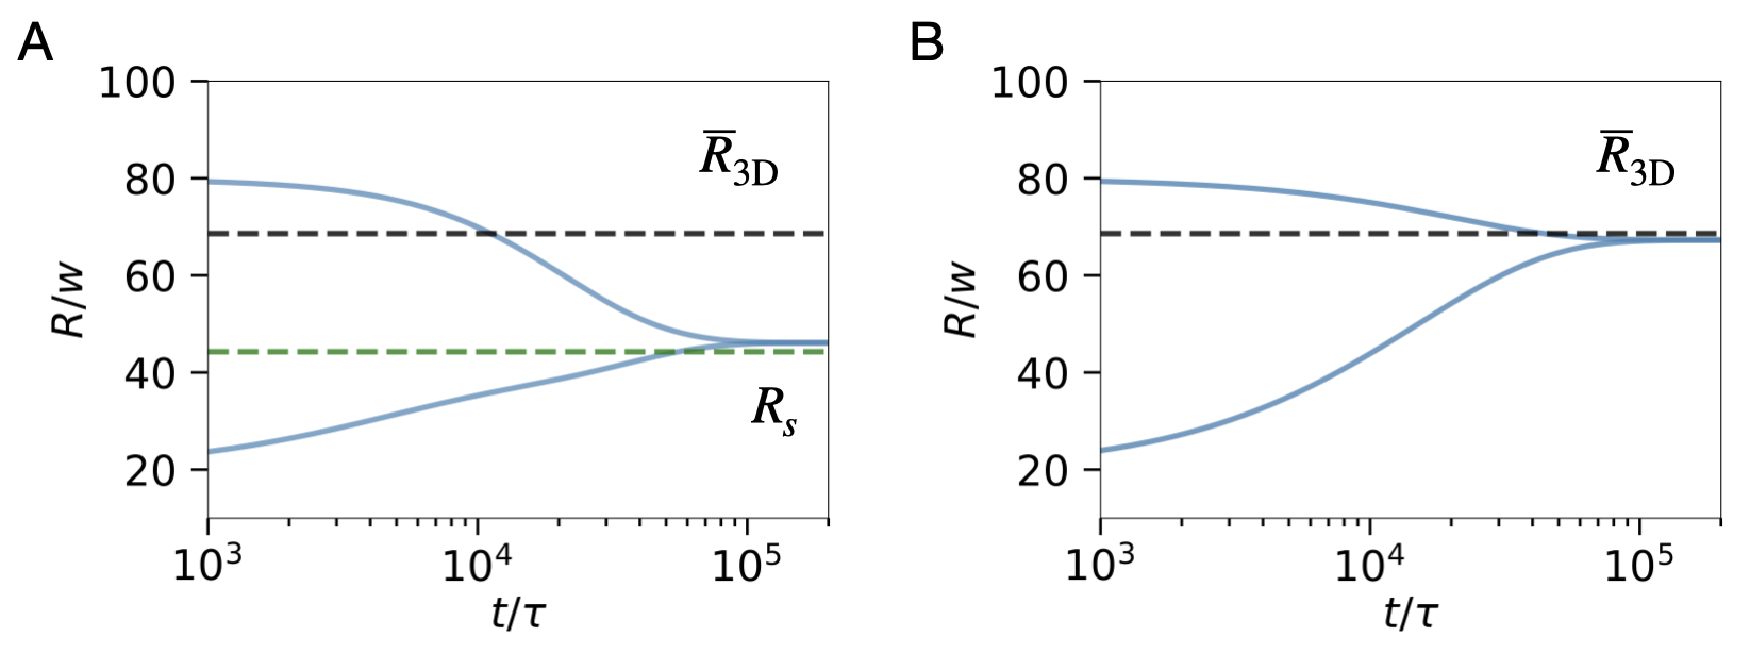
\includegraphics[scale=0.5]{MainContent/Figures/active_droplet_pair.pdf}
\caption{\textbf{Mean-field coarsening of a pair of active droplets in a finite system (A) and a large system (B).}
(A) Droplet radius $R$ as a function of time $t$ for a pair of active droplets in a finite system, which reaches a fixed size $R_s$ (dashed green line) predicted from \Eqref{eqn:approx_stable_radius_finite}, and compares well with the effective droplet model (blue).
(B) The droplet pair reaches a fixed radius $\overline{R}_\mathrm{3D}$ (dashed black line) given by numerically solving for $\jIn = \jOut$ from \Eqsref{eqn:fluxes_in_firstorder} for a large system and compares well with simulations using the effective droplet model (blue).
\mbox{(A-B)}
Simulations using the effective droplet model were carried out for a pair of droplets, of initial radius $R_0 = [20w, 80w]$ in a $3$-dimensional periodic cubic domain of size $[0, L_1]^3$ for a finite system, where $L_1 = 200 w$ and size $[0, L_2]^3$ for a large system, where $L_2 = 10^4 w$.
Model parameters are $s(\phi)= \kf (1 - \phi) - \kb \phi$, $\kf = 1 \times 10^{-5} \tau^{-1}$, $\kb = 1 \times 10^{-4}  \tau^{-1}$ and $\phiOut(t=0) = \phi_\infty$.
As $R_s$ is calculated from a mean-field approach, simulation parameters were $\dx \approx \ell \approx \ds \approx L_1$ for (A) and  $\dx \approx \ell \approx \ds \approx L_2$ for (B).
Remaining parameters are specified in Fig. \ref{fig:droplet_pair_schematics}.
}
\label{fig:active_droplet_pair}
\end{figure}
Thus our model successfully demonstrates the coarsening of a pair of droplets and agrees well with the analytical predictions and the continuous model.
Next, we consider slightly complex situations of multiple active droplets.

%%%%%%%%%%%%%%%%%%%%%%%%%%%%%%%%%%%%%%%%%%%%%%%%%%%%%%%%%%%%%%%%%%%%%%%%

\subsubsection{Coarsening of multiple active droplets in a large system}

We consider the interaction of many active droplets in a large dilute system and simulate $100$ droplets with radii uniformly chosen in $[10w, 50w]$ and placed in a periodic cubic domain of size $[0, L]^d$ with $L=1000 w$ in an initial supersaturation equal to $\phi_\infty$.

\figref{fig:active_emulsions}, \figref{fig:active_emulsion_1D} show that the emulsions with broad initial sizes quickly converge to a mono-disperse  distributions for $1, 2$ and $3$ dimensional systems.
The stable radii $\overline{R}_\mathrm{1D}, \overline{R}_\mathrm{2D}, \overline{R}_\mathrm{3D}$ are obtained from setting $\jIn = \jOut$ in \Eqsref{eqn:fluxes_in_firstorder} and they compare well with simulations using the effective droplet model.
Note that we do not use the continuous model for comparison, as it is extremely computationally costly, given the sizes of the system which we simulate. 

\begin{figure}[tb]
\centering
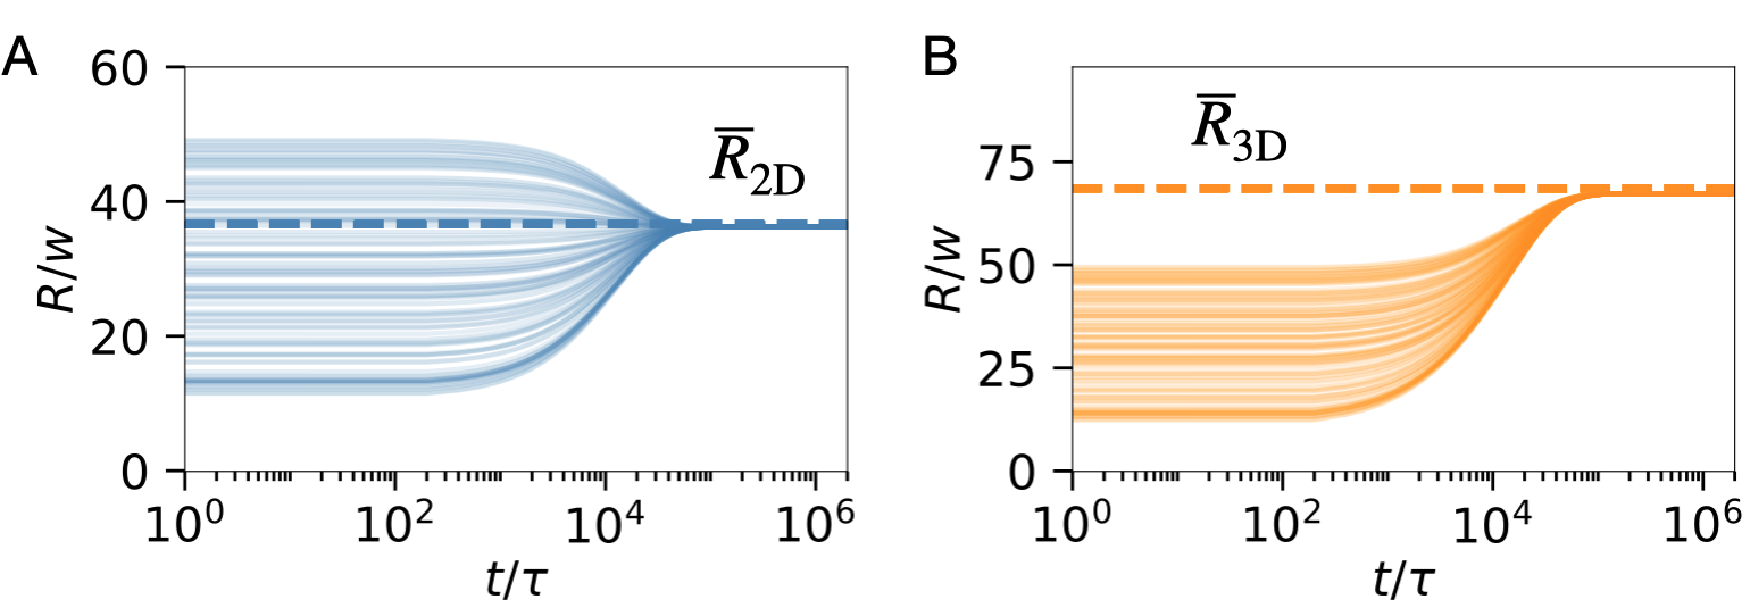
\includegraphics[scale=0.5]{MainContent/Figures/active_emulsions.pdf}
\caption{
\textbf{Suppression of \textit{Ostwald-Ripening} by first-order chemical reactions}.
%Active droplets with first-order chemical reactions attain a stationary radius based on material flux balance between incoming fluxes into the droplets and material destroyed inside the droplets.
(A, B) Radii $R$ as a function of time $t$ of droplets evolving in $d=2$ dimensions (A) and $d=3$ dimensions (B).
The theoretically expected radii are indicated by dashed horizontal lines for 2 dimensions as ($\overline{R}_\mathrm{2D}$) and for 3 dimensions as ($\overline{R}_\mathrm{3D}$). 
$\overline{R}_\mathrm{2D}, \overline{R}_\mathrm{3D}$ are obtained by numerically solving for $\jIn = \jOut$ from \Eqsref{eqn:fluxes_in_firstorder}.
$100$ droplets with radii chosen uniformly in $[10w, 50w]$ were placed in a periodic cubic domain of size $[0, L]^d$ with $L=1000 w$.
Model parameters are $s(\phi)= \kf (1 - \phi) - \kb \phi$, $\phiOut(t=0) =\phi_\infty$, $\kf = 1 \times 10^{-5} \tau^{-1}$, $\kb = 1 \times 10^{-4}  \tau^{-1}$, $\Delta x \approx \ell \approx L$, and a single shell sector for all droplets.
Remaining parameters are specified in Fig. \ref{fig:droplet_pair_schematics}.
}
\label{fig:active_emulsions}
\end{figure}

\begin{figure}[tb]
\centering
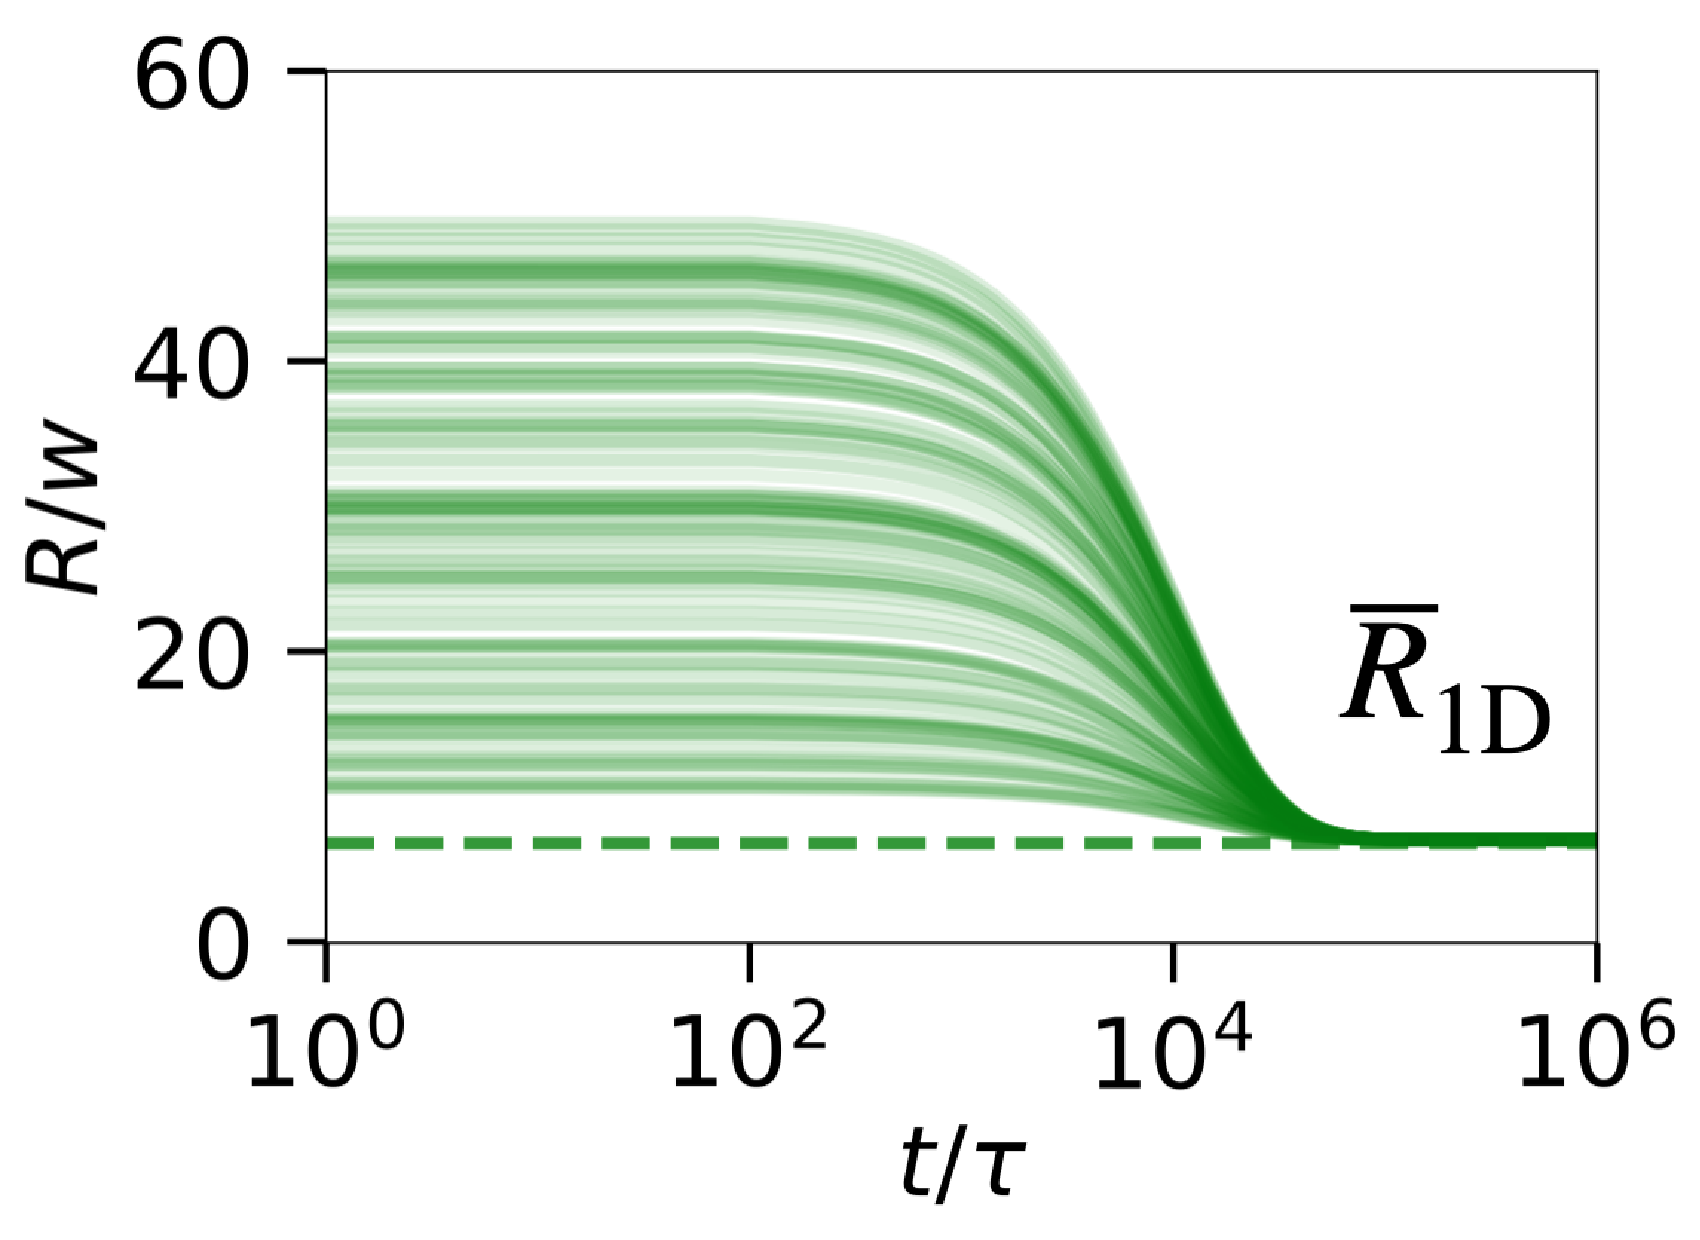
\includegraphics[scale=0.24]{MainContent/Figures/active_emulsion_1D.pdf}
\caption{
\textbf{Suppression of \textit{Ostwald-Ripening} by first-order chemical reactions in one dimension}.
Droplet radii $R$ as a function of time $t$ of active droplets evolving in $d=1$ dimension.
The theoretically expected radius is indicated by dashed horizontal line.
$100$ droplets with radii chosen uniformly in $[10w, 50w]$ are placed in a periodic one-dimensional Cartesian domain of size $[0, L]$ with $L=1000 w$.
Remaining parameters are specified in Fig. \ref{fig:active_emulsions}.
}
\label{fig:active_emulsion_1D}
\end{figure}

%%%%%%%%%%%%%%%%%%%%%%%%%%%%%%%%%%%%%%%%%%%%%%%%%%%%%%%%%%%%%%%%%%%%%%%%

\subsubsection{Coarsening of multiple active droplets in a finite system}

As a final example, we consider the interaction of many active droplets in a finite system.
It is known that multiple interacting active droplets undergoing first-order reactions typically arrange themselves in a hexagonal lattice for 2 dimensional systems; see Ref. \cite{Zwicker2015}, and as shown from simulations of the continuous model; see \figref{fig:lattice_2D_CH}.
In the steady state the droplets position themselves such that all of them share a common supersaturation $\overline{\phi}$ given by \Eqref{eqn:phi_dynamics}.
We now seek to recapitulate this phenomena using the effective droplet model.
Note that we do not simulate such systems using the continuous model, owing to prohibitive computational costs.

We simulate the effective droplet model for 10 droplets (\figref{fig:lattice_2D}A) and 40 droplets (\figref{fig:lattice_2D}C) of initial radius $R_0$ chosen uniformly in $[9.5w, 10.5w]$ in a periodic 3 dimensional system of size $[0, L]^2$, where $L = 10^3 w$.
We start with an initial background field $\phiOut(t=0) = \phi_\infty$, and the droplets grow until a stable radius is reached.
As we are primarily interested in the spatial resolution on a droplet level, we resolve $\phiOut$ on the scale of a single droplet.
This also ensures that the drift of the droplets is also captured correctly, which is an important factor in the formation of the lattice.

\begin{figure}[tb]
\centering
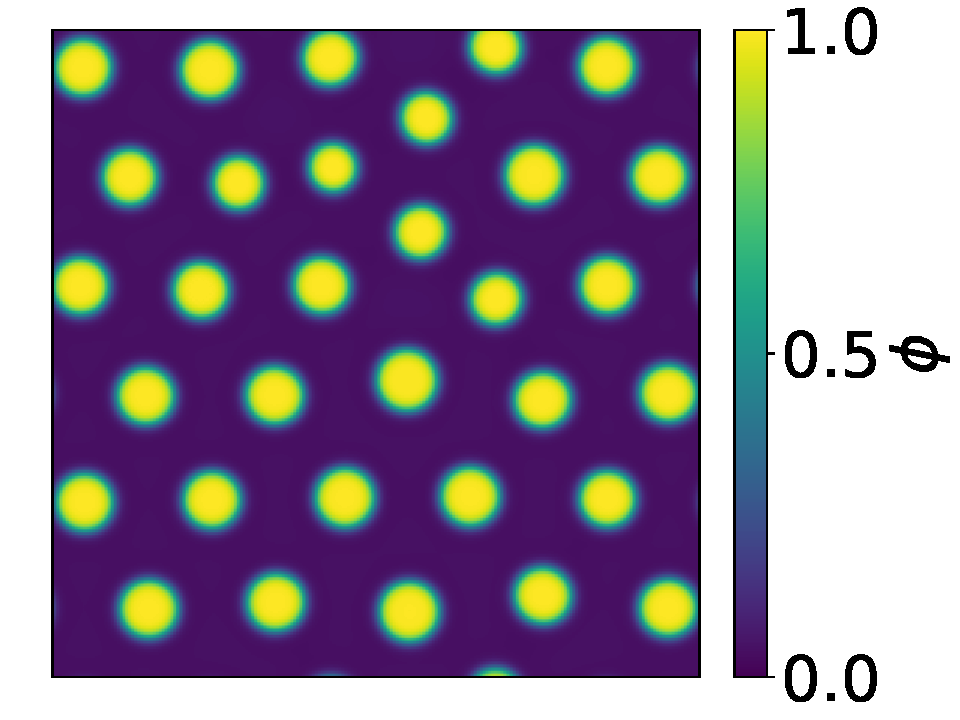
\includegraphics[scale=0.4]{MainContent/Figures/lattice_2D_CH.pdf}
\caption{\textbf{Active droplets with first order reactions forming a 2 dimensional lattice using the continuous model.}
Simulations using the continuous model shows active droplets forming a lattice in a 2 dimensional system using first-order reactions; see Ref. \cite{Zwicker2015}.
The continuous model used a $2$-dimensional periodic Cartesian domain of size $[0, L]^2$, where $L = 10^3 w$.
Model parameters are $s(\phi)= \kf (1 - \phi) - \kb \phi$, $\phi(t=0)$ is chosen as a random uniform field $\phi \in [0.1, 0.4]$ on the entire domain, $\kf = 3 \times 10^{-4} \tau^{-1}$, $\kb = 1 \times 10^{-3}  \tau^{-1}$.
Remaining parameters are specified in Fig. \ref{fig:droplet_pair_schematics}.
}
\label{fig:lattice_2D_CH}
\end{figure}

As seen from \figref{fig:lattice_2D}A and \figref{fig:lattice_2D}C, we recover this phenomena for a 2 dimensional finite system with different initial conditions consisting of increasing droplet number.
Furthermore, the stable radius $R_s$ predicted from \Eqref{eqn:approx_stable_radius_finite} agrees well with the effective droplet model, as seen from \figref{fig:lattice_2D}B and \figref{fig:lattice_2D}D, and deviates increasingly from $\overline{R}_\mathrm{2D}$ given by numerically solving for $\jIn = \jOut$ from \Eqsref{eqn:fluxes_in_firstorder}, with increasing droplet density.
This is expected, as the prediction for $\overline{R}_\mathrm{2D}$ assumes droplet density to be low.
For the simulations with low droplet density (\figref{fig:lattice_2D}A, \figref{fig:lattice_2D}B), $R_s > \overline{R}_\mathrm{2D}$ as $V_s = \pi R^2_s$ (for two dimensions) is directly proportional to the system volume $V_\mathrm{system}$ and hence will approach a large number as the system size $L \rightarrow \infty$.
Consequently, for simulations with high droplet density (\figref{fig:lattice_2D}C, \figref{fig:lattice_2D}D), $R_s < \overline{R}_\mathrm{2D}$ as $\overline{R}_\mathrm{2D}$ assumes the system size to be large. 
This interesting interplay between $R_s, \overline{R}_\mathrm{2D}$ is also seen from \figref{fig:lattice_2D}B, \figref{fig:lattice_2D}D.
Taken together, we in this section, we demonstrated that our effective model faithfully recovers important physical behaviour of active droplets.

\begin{figure}[tb]
\centering
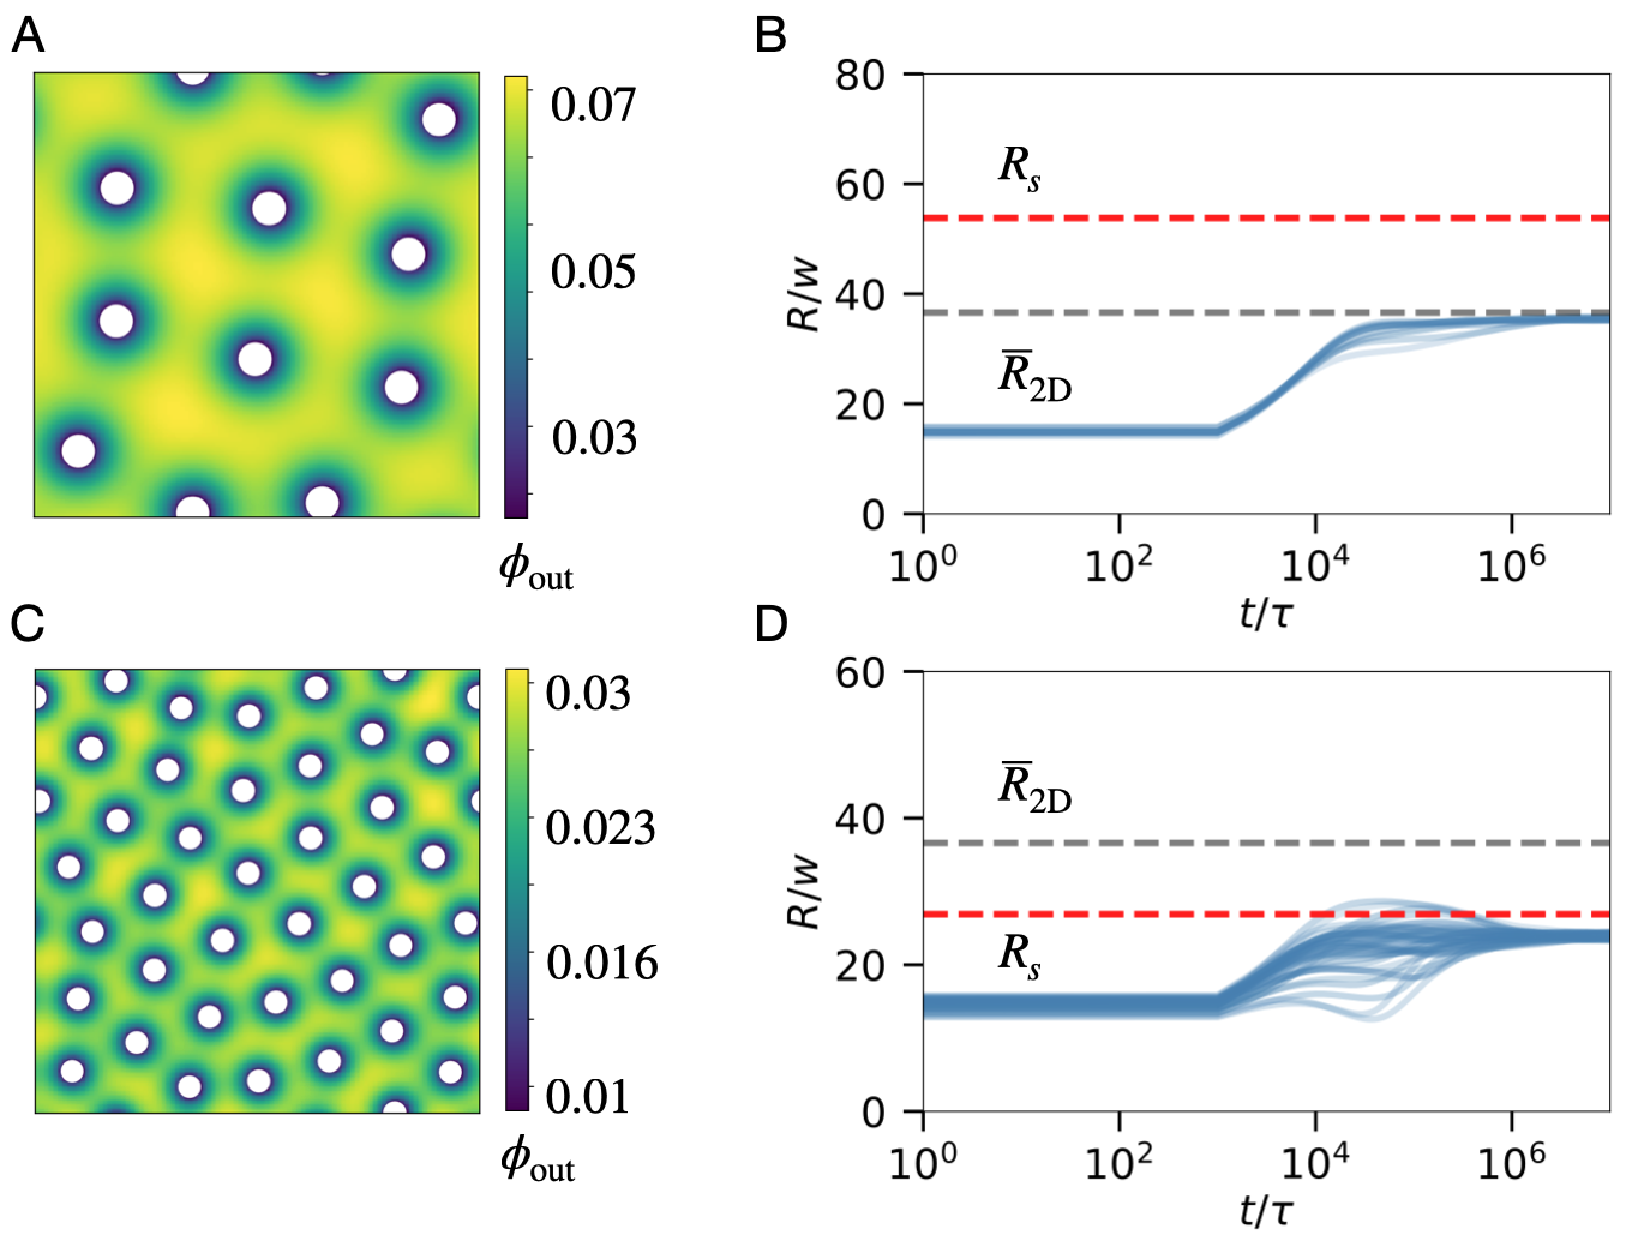
\includegraphics[scale=0.5]{MainContent/Figures/lattice_2D.pdf}
\caption{\textbf{Active droplets with first order reactions forming a two dimensional lattice using the effective droplet model.}
Active droplets with first-order chemical reactions attain a stationary radius and form a lattice in 2 dimensional systems using the effective droplet model.
(A) and (C) show 10 and 40 active droplets with radii chosen uniformly in $[9.5w, 10.5w]$ and placed in a periodic Cartesian domain of size $[0, L]^2$ with $L=10^3 w$.
(B) and (D) show droplet radius $R$ with time and a good agreement of the stable radius from the effective droplet model with the theoretically predicted $R_s$ (dashed red line) from \Eqref{eqn:approx_stable_radius_finite}. 
$\overline{R}_\mathrm{2D}$ (dashed black line), given by numerically solving for $\jIn = \jOut$ from \Eqsref{eqn:fluxes_in_firstorder}, deviates increasingly from $R_s$, for increasing droplet densities.
Model parameters are $s(\phi)= \kf (1 - \phi) - \kb \phi$, $\phiOut(t=0) =\phi_\infty$, $\kf = 1 \times 10^{-5} \tau^{-1}$, $\kb = 1 \times 10^{-4}  \tau^{-1}$, $\Delta x \approx \ds \approx \ell \approx R_0$.
Remaining parameters are specified in Fig. \ref{fig:droplet_pair_schematics}.
}
\label{fig:lattice_2D}
\end{figure}

\section{Summary}

In the last chapter; Chapter \ref{chap:Chapter_4}, we formulated the effective droplet model in detail which governs droplet dynamics according to \Eqsref{eqn:DropletDiscretized} and the dynamics of the background field $\phiOut$ using \Eqref{eqn:RD_dilute}.
We then put forward the numerical algorithm; see Algorithm \ref{alg:algorithm}, and used a test-case of a pair of identical passive droplets shrinking in a vanishing volume fraction to conclude that the optimum values for the effective droplet model are $[\dx \approx \ell \approx \ds]$.

In this chapter, we validated our claim of optimum simulation parameters for the effective droplet model by comparing it with known analytical results from literature and simulations using the continuous model (wherever computationally viable).
We were motivated from biology, in particular, simulating two mechanisms the cell potentially uses to regulate the dynamics of condensates - chemical reactions and external chemical gradients.
To help disentangle the individual roles of these two mechanisms, we considered them separately; first in simulations of single droplet systems, and then through simulations of many droplet systems. 

We started by considering simple scenarios involving a single droplet and moved to more complex situations, eventually reaching a point where we simulated coarsening behaviour of $10^5$ droplets.
As our aim was to simulate dynamics of phase separated droplets accurately, throughout all the simulation scenarios, we primarily focused on comparing droplet growth and drift.
Wherever possible, we derived the equations for growth (and drift) of the droplets using the thin-interface approximation given by \Eqsref{eqn:thin_interface_model}.

First, we simulated a passive droplet growing in a large supersaturated system and simulations using the continuous model, the effective droplet model with optimum parameters and analytical predictions; see Refs. \cite{Review2019,Weber2017}, match well; see \figref{fig:passive_droplet}.
Next, we validated the effective droplet model for a passive droplet in an external volume fraction gradient; see \figref{fig:drop_in_gradient} and tested the effective droplet model for this scenario for simulation parameters other than the optimum values, thus highlighting the importance of choosing the correct values for the simulation parameters; see \figref{fig:drop_in_gradient_all}.

We then moved on to demonstrate the hallmark of this model - the ability to simulate large scale emulsions of many droplets. 
To this end, we simulated \textit{Ostwald-Ripening}; see \figref{fig:passive_emulsions}, and the effective droplet model accurately captured the $t^{\,1/3}$ scaling of the mean droplet radii; see Refs. \cite{Review2019,LSWanalytics}.
Note that we did not simulate \textit{Ostwald-Ripening} with the continuous model, as the system sizes we chose would have been prohibitively costly.

All of the above simulations were representative examples of droplets in passive phase separation. 
We then introduced (weak) first-order chemical reactions and successfully validated it's effects on droplet dynamics using the effective droplet model for various scenarios.
The situations we considered were: a) Single active droplet in a finite system and a large system reaching a stable radius; see \figref{fig:active_droplet_3D} and \figref{fig:active_droplet_2D_infinite}, b) A pair of active droplets in a finite system and a large system reaching a common stable radius; \figref{fig:active_droplet_pair}, and c) Many active droplets in a finite system and a large system reaching a common stable radius; see \figref{fig:active_emulsions} and \figref{fig:active_emulsion_1D}.
Furthermore, we were also successful in recovering an ordered state for many active droplets in two dimensions, using the effective droplet model and thus demonstrating suppression of \textit{Ostwald-Ripening}; see \figref{fig:lattice_2D}.
In all the above scenarios, we reported that the effective droplet model accurately captured the growth (and drift) of droplets, as well as large scale coarsening events.

Taken together, we thus demonstrated that our effective model faithfully recovers important physical behaviour of passive and active droplets.
Furthermore, it is able to capture and disentangle the effects of chemical gradients and chemical reactions on droplet dynamics, optionally even beyond the mean-field regime by increasing the spatial resolution to capture correlations in droplet growth.


\clearpage

% Chapter 6

\onehalfspacing

\chapter{Conclusion and outlook}

\label{chap:Chapter_6}

In this thesis, we developed a fast and efficient numerical model to simulate dynamics of phase separated droplets in large-scale emulsions in the presence of chemical reactions and chemical gradients, circumventing the need of solving the computationally expensive \textit{Cahn-Hilliard} equation; see Refs. \cite{Review2019,CahnHilliardEq,Cahn1958}, describing phase separation.
We were motivated from numerous examples from biology, specifically biological cells, which need to organize their intracellular environment in a precisely regulated spatiotemporal manner to properly function and survive.
One way the cell achieves this is through manufacturing membrane-less organelles (or condensates) in an energetically efficient way using Liquid-liquid phase separation.
Additionally, aberrant condensates; which form via poor spatiotemporal regulation by the cell, are implicated in many diseases, a few being: familial amyotrophic lateral sclerosis (fALS), frontotemporal lobar degeneration (FTLD); see Ref. \cite{QAMAR2018720}, amyotrophic lateral sclerosis (ALS); see Ref. \cite{Mateju2017} and Alzheimer’s disease; see Refs. \cite{Williams2006,Mucke2009}.
This precise control of the cell over it's condensates is thought to be accomplished through various mechanisms, a few being: utilizing chemical gradients, chemical reactions via PTMs, regulating pH and temperature, physically modifying it's internal environment through forming networks and using pickering agents to modify the surface properties of the condensates.

We were interested disentangling and separately investigating the roles of two important mechanisms out of the above, namely chemical reactions and external chemical gradients, through numerical simulations of dynamics of phase separated droplets.
However, simulating the traditional \textit{Cahn-Hilliard} equation of phase separation (continuous model given by \Eqref{eqn:CHActive}) for large systems in three dimensions is prohibitively costly, as small time steps and fine grid discretizations have to be used.
Earlier works have improved the computational speeds of this model using approaches such as using multi-grid methods; see Ref. \cite{Lee2021_CH_model}, finite element modelling; see Refs. \cite{zhou2015, Chen2021}, incorporating meshless methods; see Ref. \cite{MOHAMMADI2019919} and adaptive grids; see Refs. \cite{BANAS20082,Ceniceros2007}, to overcome the challenges posed, but the fundamental drawbacks still persist.

However, since we are interested primarily in modelling dynamics of droplets, we circumvented these problems by focusing only on phase separation inside the nucleation and growth regime, and assuming that sufficiently finite perturbations have already nucleated droplets.
We discussed the thin-interface approximation; see \Eqsref{eqn:thin_interface_model}, which was a coarse-grained analytical formulation of the continuous model subject to strong phase separation, low variation of volume fractions in the droplet phase and the dilute phase themselves and large droplet sizes compared to the interface width.
This approximation describes dynamics of droplets and dynamics of the dilute phase separately, instead of the full volume fraction field from the continuous model; see \figref{fig:schematics}, thus effectively `de-coupling' the description of phase separated droplets from the dilute phase.
This analytical approach was utilized by Zwicker et al. \cite{Zwicker2015} to study kinetics of many droplet systems and effects of chemical reactions on such systems.

The aim of this thesis was to then utilize the thin-interface approximation, build a numerical model (the effective droplet model) upon it to simulate the dynamics of phase separated droplets in presence of chemical reactions and external chemical gradients, and thus obtain insights how the cell is able to robustly regulate the size and shape of the condensates in spite it's complex intracellular environment which experiences thousands of biomolecular reactions every second.
Using the thin-interface approximation, we built up the effective droplet model systematically and chose optimum values for various simulation parameters based on comparisons with simulations using the continuous model.
We then demonstrated that the effective droplet model captures droplet dynamics accurately for two extreme scales, namely a) simple scenarios typically involving a single droplet or a pair of droplets and b) \textit{Ostwald-Ripening} of $10^5$ droplets, where it accurately replicates the theoretical predictions for the $t^{1/3}$ scaling of the mean radius from Refs. \cite{LSWanalytics,Lifshitz}.
In addition, we studied the roles of two important mechanisms that influence the physics of phase separation - chemical reactions and external chemical gradients on droplet dynamics, by simulating them individually and thus disentangling their effects on growth and drift of droplets.

We now reasonably assume that with optimum choices for the simulation parameters; as described in Chapter \ref{chap:Chapter_4}, intermediate-scale scenarios (which are computationally expensive to be simulated using the continuous model), for example, many-droplet systems in the presence of chemical reactions and chemical gradients, should also be captured well using the effective droplet model, which we will demonstrate and discuss next.

\section{Droplet dynamics in the presence of chemical reactions and external volume fraction gradient}

We now present the final demonstration of the effective droplet model, where we simulate the combined effect of chemical reactions and external volume fraction gradients on the dynamics of the droplets; see \figref{fig:active_emulsion_gradient}.
We simulate many active droplets in a large three dimensional system and the droplets are immersed in an external volume fraction gradient (along one dimension) of the droplet material.
Based on results from Chapter \ref{chap:Chapter_5}, we expect the droplets to drift in the direction of the gradient.
Additionally, as seen from Chapter \ref{chap:Chapter_5}, droplets with first-order reactions (and in the absence of an external gradient) attain a stable radius $\overline{R}_\mathrm{3D}$ in three dimensions, which is based on flux balances and given by numerically solving for $\jIn = \jOut$ from \Eqref{eqn:fluxes_in_firstorder}.
Hence, we hypothesize the following: if we want to achieve \textit{both}: stable radii (size control) and droplet drift (position control) for the droplets, chemical reactions and external chemical gradients might be the right combination to materialize such a situation. 

To investigate our claim, we now simulate four droplets with radii chosen uniformly in $[0.8 \left \langle R_0 \right \rangle, 1.2 \left \langle R_0 \right \rangle]$, where $\left \langle R_0 \right \rangle = 40w$.
The droplets are placed in cubic domain of size $[0, L]^3$ with $L = 10^3 w$ with $\dx \approx \ell \approx \Delta s \approx \left \langle R_0 \right \rangle$; see \figref{fig:active_emulsion_gradient}, along with the boundary conditions $\phiOut(x = -L/2) = 0$ and $\phiOut(x = L/2) = 0.1$ to maintain the one-dimensional gradient and no-flux boundary conditions at the remaining system boundaries.
\begin{figure}[tb]
\centering
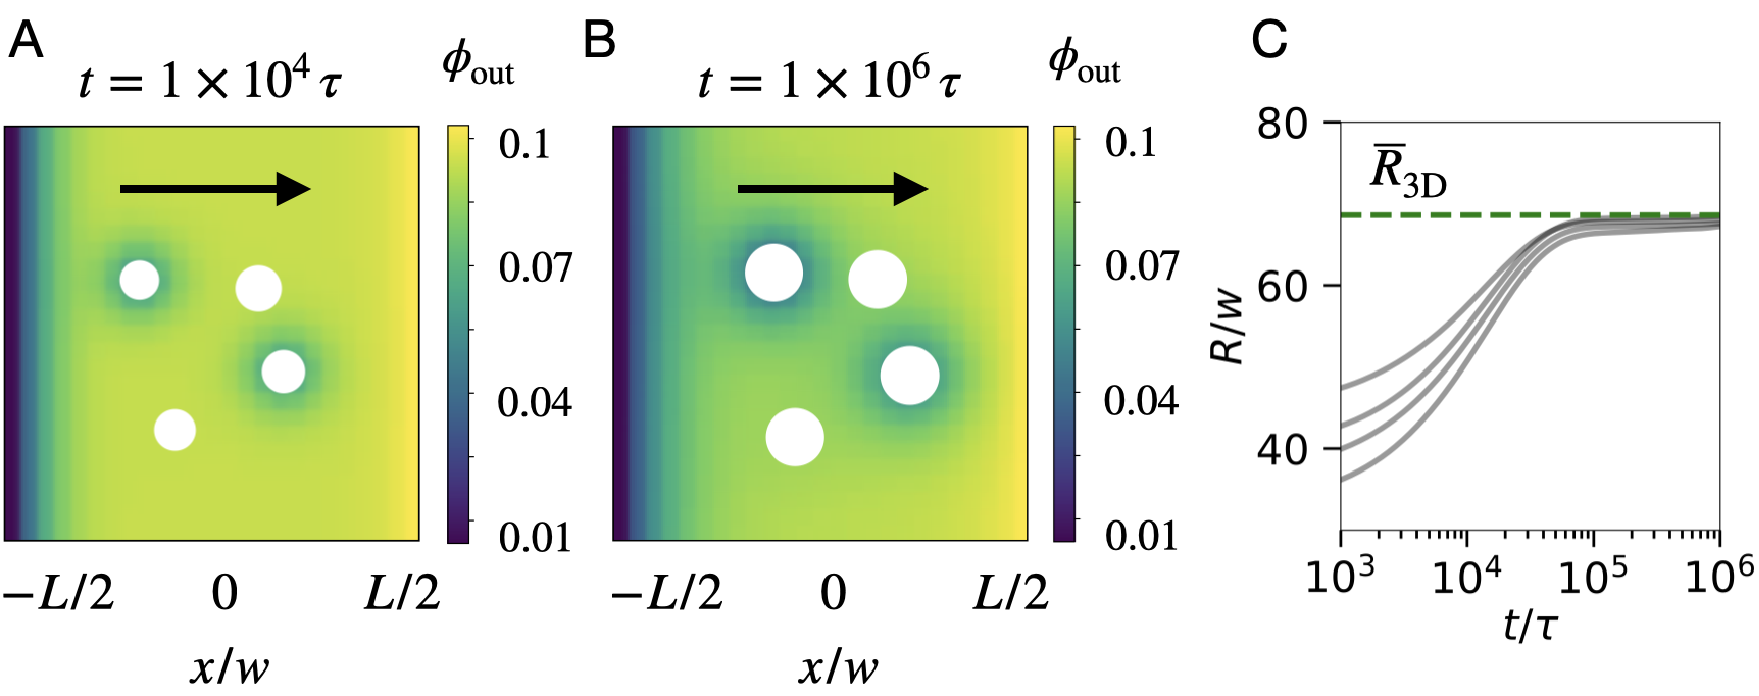
\includegraphics[scale=0.52]{MainContent/Figures/active_emulsion_gradient.pdf}
\vspace{10pt}
\caption{\textbf{Active droplets ripening along external gradients in three dimensional systems.}
Figure shows ripening of active droplets in three dimensional systems at intermediate snapshots, using effective droplet model. Droplets (white circles) are shown as two dimensional projections and arrow shows the direction of the gradient along which the droplets grow and drift.
\mbox{(A-B)} Active droplets with first-order chemical reactions under the influence of an external volume fraction (one-dimensional) gradient grow towards a fixed size and drift towards the gradient direction, thus qualitatively depicting spatiotemporal size control of biomolecular condensates.
The gradient is maintained only along the $x$ direction through boundary conditions.
(C) Droplet radius $R$ as a function of time $t$ for different droplets approaching a fixed size $\overline{R}_\mathrm{3D}$ (dashed line), which is obtained from numerically solving for $\jIn = \jOut$ from \Eqsref{eqn:fluxes_in_firstorder}; ; compare to \figref{fig:active_emulsions}.
4 droplets with radii chosen uniformly in $[0.8 \left \langle R_0 \right \rangle, 1.2 \left \langle R_0 \right \rangle]$, where $\left \langle R_0 \right \rangle \approx 40 w$ are placed in cubic Cartesian domain of size $[0, L]^3$ with $L = 10^3 w$ with $\dx \approx \ell \approx \Delta s \approx \left \langle R_0 \right \rangle$ along with the boundary conditions $\phiOut(x = -L/2) = 0$ and $\phiOut(x = L/2) = 0.1$ and no-flux boundary conditions at the remaining system boundaries.
Model parameters are $s(\phi)= \kf (1 - \phi) - \kb \phi$, $\phiOut(t=0) =\phi_\infty$, $\kf = 1 \times 10^{-5} \tau^{-1}$ and $\kb = 1 \times 10^{-4} \tau^{-1}$.
Remaining parameters are specified in Fig. \ref{fig:droplet_pair_schematics}.
}
\label{fig:active_emulsion_gradient}
\end{figure}
Indeed as seen from \figref{fig:active_emulsion_gradient}, we observe that droplets (shown as two dimensional projections) grow as they drift along the (one dimensional) gradient \textit{and} they approach the fixed radius given by $\overline{R}_\mathrm{3D}$, thus achieving both - size control and droplet drift.
Thus, through simulations of the effective droplet model, we are able to qualitatively demonstrate spatiotemporal size control of biomolecular condensates, where precise location and size is controlled by the cell potentially through chemical gradients and chemical reactions; see Refs. \cite{Brangwynne2009,Brangwynne2013}.

\section{Future extensions to the effective droplet model}

Having modelled the effects of chemical reactions and external chemical gradients on droplet dynamics, we now discuss and propose future improvements for the effective droplet model.
This model has been extended to integrate elasticity and utilized by Vidal-Henriquez et al. \cite{VidalHenriquez2021,Vidal2020} to study droplet ripening in passive emulsions with the presence of an elastic matrix.
This is a valuable extension to the model, as cells are thought to utilize chromatin networks to suppress coalescence of condensates and thus stabilizing them; see Refs. \cite{Feric2013,Wiegand2020,Boeddeker2022}.
Additional extensions such as fluid flows which are pertinent to biological cells; see Refs. \cite{Brangwynne2009,Setru2021,Brangwynne2011}.
In particular, Seyboldt et al. \cite{Seyboldt_2018} investigated the role of hydrodynamic flows in stabilizing droplets in presence of strong chemical reactions.
Fluid flows can be incorporated by including advection terms in the dynamics of volume fractions inside the droplets and in the background field.

Further, we currently have ignored the effects of droplet splitting and coalescence.
Coalescence can be incorporated in the model through volume conservation of droplets touching each other.
Inside biological cells, condensates have been shown to exhibit anomalous coarsening behaviour, primarily due to hindrance and physical barrier which curb their ability of coalesce; see Refs. \cite{Feric2013,Quiroz2020,Boeddeker2022,Lee2021}.
Thus including the effects of droplet coalescence in the model will be a useful extension.
Droplet splitting along with non-spherical droplets will also be a valuable addition to the model, as it is relevant when considering strong chemical reactions; see Refs. \cite{Zwicker_nature_2016,Seyboldt_2018}.

Taken together, we demonstrated that the effective droplet model faithfully captures the effects of chemical reactions and external chemical gradients on droplet dynamics.
Additionally, the gain in computational speed of the effective droplet model is shown to be orders of magnitude faster than simulations of the continuous model given by \Eqref{eqn:CHActive} for similar systems, making it a viable and a pragmatic option for fast and computationally efficient simulations of phase separated droplets in large many-droplet emulsions.
Most importantly, our model can be used as a modular platform, which can be extended to include other relevant physical phenomena which play a role in controlling condensate dynamics, thus shedding insights on the formation, dissolution, stability and sizes of biomolecular condensates.

\clearpage

% Appendices

\begin{appendices}

\addtocontents{toc}{\protect\renewcommand{\protect\cftchappresnum}{\appendixname\space}}
\addtocontents{toc}{\protect\renewcommand{\protect\cftchapnumwidth}{7em}}

%%%%%%%%%%%%%%%%%%%%%%%%%%%%%%%%%

\chapter{Instabilities of the homogeneous state}

\label{sec:phasesep}

We briefly examine the stability of the homogeneous state when it is introduced in the two regimes from \figref{fig:free_energy}, namely the nucleation and growth regime and the spinodal decomposition regime, and prove that a necessary condition for spontaneous phase separation is $f''(\phi) < 0$, i.e. regions where $f(\phi)$ is convex.
Here $f(\phi)$ is the free energy density given by \Eqref{eqn:free_energy_formulation} or \Eqref{eqn:free_energy}, as both of the free energy densities exhibit identical behaviour for stability of the phases; see Ref. \cite{Review2019}.

\section{Spinodal decomposition regime}

We first focus on the spinodal decomposition regime, where infinitesimal fluctuations in the homogeneous state are unstable, thus promoting phase separation into the minima described by the free energy density. 
We start by assuming in an homogeneous state, small perturbations lead to the formation of two phase separated domains, each of volume $\delta V$.
The resulting volume fractions for the two domains read as $\phi_1 = \phi - \delta \phi$ and $\phi_2 = \phi + \delta \phi$, as mass conservation dictates that the average volume fraction $\phi$ must remain constant.
The free energy change in this case can be calculated as: 
\begin{equation*}
    \delta F = \delta V f(\phi_1) + \delta V f(\phi_2) - 2 \delta V f(\phi) = \delta V (\delta \phi)^2 f''(\phi).
\end{equation*}
Thus, we see that if $f''(\phi) < 0$ (i.e. $f(\phi)$ is convex), the infinitesimal perturbations are energetically favourable and will grow.
This regime is commonly referred to as the Spinodal decomposition; see \figref{fig:free_energy}.
Consequently,  $f''(\phi) > 0$ implies that the perturbations will die down, making phase separation energetically unfavourable for infinitesimal perturbations.
We will now see the conditions for phase separation to be initiated in the region where $f(\phi)$ is concave. 

\section{Nucleation and growth regime}

We now focus on the nucleation and growth regime and see the conditions for which the perturbations in this regime grow.
As infinitesimal perturbations in this regime die down quickly, we explore what happens when we have finite perturbations.

Let us assume the finite perturbation to be of the kind where a droplet of radius $R$ forms and the volume fraction in the dilute phase $\phiOut$ changes by an amount $\delta \phi$, where $\delta \phi \ll \phi$.
From \Eqref{eqn:constraint_3}, the free energy change in this case can be calculated as: 
\begin{equation}
\label{eqn:infinitesimal_change_0}
    \delta F = V_d f(\phiIn) + (V - V_d) f(\phi - \delta \phi) - V f(\overline{\phi}) + S \gamma,
\end{equation}
where we used $\phiOut = \phi - \delta \phi$, $V$ is the volume of the system, $V_d = (4/3) \pi R^3$ is the volume of the droplet, $S = 4 \pi R^2$ is the surface area and $\overline{\phi}$ is the average volume fraction. 
Similarly, from \Eqref{eqn:constraint_4}, we have $V_d \, \phiIn + (V - V_d) (\phi - \delta \phi) = V \overline{\phi}$.
Thus, we calculate the change in volume fraction $\delta \phi$ as:
\begin{equation}
\label{eqn:infinitesimal_change_1}
    \delta \phi = \phi - \frac{V \overline{\phi} - V_d \phiIn}{V - V_d}.
\end{equation}
Expanding $\delta \phi$ from \Eqref{eqn:infinitesimal_change_1} in linear order, we have from \Eqref{eqn:infinitesimal_change_0},
\begin{equation}
\label{eqn:infinitesimal_change_2}
    \delta F \approx V_d [f(\phiIn) - f(\phi) - f'(\phi)(\phiIn - \phi)] + S \gamma.
\end{equation}
From \Eqref{eqn:infinitesimal_change_2}, we can qualitatively see that the term $S \gamma \, (\sim R^2)$ will dominate for small radius and thus increasing the droplet radius further is not energetically favourable. 
On the other hand for large radius, the term proportional to $V_d$ will dominate ($\sim R^3$). 
Hence, if the droplet is larger than a critical radius $R_c$, it will further lower the free energy as it increases in size.
We can calculate this critical radius by setting $\partial_R\,\delta F = 0$, which gives us:
\begin{equation*}
    R_c = (2 \gamma) / [f(\phiIn) - f(\phi) - f'(\phi)(\phiIn - \phi)].
\end{equation*}
Note that the critical radius $R_c$ is proportional to the surface tension $\gamma$.
We hence prove that in the nucleation and growth regime, sufficiently finite perturbations are required to initiate phase separation and form droplets. 

%%%%%%%%%%%%%%%%%%%%%%%%%%%%%%%%%

\chapter{Droplet dynamics for spherical droplets}

\label{sec:droplet_dynamics}

Here, we derive the equations for the growth speed and drift rate of droplets of arbitrary shape described by \Eqsref{eqn:droplet_dynamics} in two and three dimensions; see Refs. \cite{Review2019,Weber2017}.
% The general shape of a droplet is described by its surface $\Omega$.
% Assuming that the 2 dimensional surface of a 3 dimensional droplet (and correspondingly the 1 dimensional curve of a 2 dimensional droplet) does not deviate a lot from it's spherical shape, we place a spherical co-ordinate system centered on the droplet in 3 dimensions (and a polar co-ordinate system in 2 dimensions).

% The position vector of the droplet surface can be defined as $\vec{R}(\theta, \varphi,t) = P(\theta, \varphi,t) \, \vec{e}_{\mathrm{r}}$ in 3 dimensions and $\vec{R}(\theta, t) = P(\theta,t) \, \vec{e}_{\mathrm{r}}$ in 2 dimensions, where $P$ is the surface parameterization of the droplet surface at time $t$.
% The interfacial velocity $\vec{v}$ can then be split into radial and normal components to the droplet surface as $v_\mathrm{n}$ and $v_\mathrm{r}$.
% From geometry, it follows that $v_\mathrm{r} ~ \vec{e}_\mathrm{r} \cdot \vec{n} = v_\mathrm{n}$, where $\vec{r}, \vec{n}$ are the interfacial velocities in the outward radial and normal directions respectively.

% Droplet growth rate follows from rate of change of volume of the droplet, which we calculate next. 
% The volume of the drop is defined as:
% \begin{subequations}
% \begin{align}
%     V_\mathrm{3D} &=\int_{\theta} \int_{\varphi} \int_{r}  \, r^2 \sin\theta \,  \mathrm{d}\theta  \, \mathrm{d}\varphi \,  \mathrm{d}r = (1 / 3) \int_{\theta} \int_{\varphi} P(\theta, \varphi, t)^3 \, \sin\theta \,  \mathrm{d}\theta  \, \mathrm{d}\varphi \nonumber \mathrm{~and~}
%     \\[10pt]
%     V_\mathrm{2D} &= \int_{\theta} \int_{r} r\,\mathrm{d}r \, \mathrm{d}\theta = (1 / 2) \int_{\theta} P(\theta, t)^2 \,\mathrm{d}\theta, \nonumber
% \end{align}
% \end{subequations}
% where, throughout this section, the subscripts $\mathrm{2D/3D}$ indicate in 2 dimensions and in 3 dimensions respectively. 
% The rate of volume change reads as:
% \begin{subequations}
% \begin{align}
%     \partial_t V_\mathrm{3D} &= \int_{\theta} \int_{\varphi} P(\theta, \varphi, t)^2  \, \partial_t P(\theta, \varphi, t) \,  \sin\theta \,  \mathrm{d}\theta \,  \mathrm{d}\varphi \nonumber \mathrm{~and~}
% 	\\[10pt]
% 	\partial_t V_\mathrm{2D} &= \int_{\theta} P(\theta, t) \,  \partial_t P(\theta, t) \,\mathrm{d}\theta. \nonumber
% \end{align}
% \end{subequations}

% % Alternatively, we also note that $\partial_t V_\mathrm{2D/3D} = S_\mathrm{2D/3D}~\partial_t M_\mathrm{2D/3D}$, where $S_\mathrm{2D/3D}$ is the surface area of the droplet and $M_\mathrm{2D/3D}$ is the volume averaged radius of the droplet at time $t$ in 2 and 3 dimensions respectively.

% Alternatively, we also note that $\partial_t V_\mathrm{2D/3D} = S_\mathrm{2D/3D}~\partial_t M_\mathrm{2D/3D}$, where $S_\mathrm{2D/3D}$ is the surface area of the droplet and $M_\mathrm{2D/3D}$ is the volume averaged radius of the droplet in 2 and 3 dimensions respectively.
% Equating the two expressions for $\partial_t V_\mathrm{2D/3D}$, we have:
% \begin{subequations}
% \begin{align}
%     \partial_t M_\mathrm{3D} &= S^{\,-1}_\mathrm{3D} \,  \int_{\theta} \int_{\varphi} P(\theta, \varphi, t)^2  ~ \partial_t P(\theta, \varphi, t) \,  \sin\theta \,  \mathrm{d} \theta \,  \mathrm{d}\varphi \nonumber \mathrm{~and~}
% 	\\[10pt]
%     \partial_t M_\mathrm{2D} &= S^{\,-1}_\mathrm{2D} \, \int_{\theta} P(\theta, t) ~  \partial_t P(\theta, t) \,\mathrm{d}\theta. \nonumber
% \end{align}
% \end{subequations}
% Finally, assuming a spherical droplet at all times, i.e. $P(\theta, \varphi, t) = M_\mathrm{3D}$ and $P(\theta, t) = M_\mathrm{2D}$, we have:
% \begin{subequations}
% \begin{align}
%     \partial_t M_\mathrm{3D} &= (1 / 4 \pi) \int_{\theta} \int_{\varphi} \partial_t P(\theta, \varphi, t) \,  \sin\theta \,  \mathrm{d}\theta \, \mathrm{d}\varphi \nonumber \mathrm{~and~}
% 	\\[10pt]
%     \partial_t M_\mathrm{2D} &= (1 / 2 \pi) \int_{\theta} \partial_t P(\theta, t) \,  \mathrm{d}\theta, \nonumber
% \end{align}
% \end{subequations}
% which in fact becomes \Eqref{eqn:DropletGrowth} when the integral is considered over the droplet surface.

% Furthermore, the centroid of the droplet can be calculated as:
% \begin{subequations}
% \begin{align}
%     C_\mathrm{3D} &= \left[\int_{\theta}\int_{\varphi}\int_{r} \,  (r^2 \,  \sin\theta \,  \mathrm{d}\theta \,  \mathrm{d}\varphi \, \mathrm{d}r )  \, ( r \, \vec{e_p} \cdot \vec{e_r}) \right] \bigg/ \left[\int_{\theta} \int_{\varphi} \int_{r} \mathrm{d} V_\mathrm{3D} \right] \nonumber \mathrm{~and~}
% 	\\[10pt]
%     C_\mathrm{2D} &= \left[\int_{\theta} \int_{r} (r\,\mathrm{d}r \, \mathrm{d}\theta) \, (r \, \vec{e_p} \cdot \vec{e_r}) \right] \bigg/ \left[\int_{\theta} \int_{r} \mathrm{d} V_\mathrm{2D}\right], \nonumber
% \end{align}
% \end{subequations}
% where $\vec{e_p}$ is the co-ordinate along which calculating the centroid is desired.
% Following the same procedure used to calculate rate of volume change, we obtain the droplet drift speed as:
% \begin{subequations}
% \begin{align}
%     \partial_t C_\mathrm{3D} &= V^{\,-1}_\mathrm{3D} \int_{\theta} \int_{\varphi} P(\theta, \varphi, t)^3 ~ \partial_t P(\theta, \varphi, t)  \, \vec{e_p} \cdot \vec{e_r} \, \sin\theta \mathrm{d} \theta \,  \mathrm{d}\varphi \nonumber \mathrm{~and~}
% 	\\[10pt]
%     \partial_t C_\mathrm{2D} &= V^{\,-1}_\mathrm{2D} \int_{\theta} P(\theta, t)^2  ~  \partial_t P(\theta, t) \, \vec{e_p} \cdot \vec{e_r} \, \mathrm{d} \theta. \nonumber
% \end{align}
% \end{subequations}

% Hence, we get
% \begin{subequations}
% \begin{align}
%     \partial_t C_\mathrm{3D} &= (3 / 4 \pi) \int_{\theta} \int_{\varphi} \partial_t P(\theta, \varphi, t) \, \vec{e_p} \cdot \vec{e_r} \, \sin\theta \,  \mathrm{d} \theta \,  \mathrm{d}\varphi \nonumber \mathrm{~and~}
% 	\\[10pt]
%     \partial_t C_\mathrm{2D} &= (1 / \pi) \, \int_{\theta} \partial_t P(\theta, t)  \, \vec{e_p} \cdot \vec{e_r} \, \mathrm{d} \theta, \nonumber
% \end{align}
% \end{subequations}
% which becomes \Eqref{eqn:DropletDrift} when the integral is evaluated over the surface of the droplet in 2 and 3 dimensions, and we arrive at \Eqsref{eqn:droplet_dynamics} describing droplet dynamics.
For simplicity, we focus on $d=3$ dimensions, but the derivation works analogously in all dimensions.
The 2D surface of a 3D droplet can be parameterized by points $\vec{R}(\theta, \varphi)$ with parameters $\theta$ and $\varphi$.
For simplicity, we consider droplet shapes that are star domains, so we can place a spherical coordinate system inside the droplet and write $\vec{R}(\theta, \varphi,t) = P(\theta, \varphi, t)  \vec{e}_r$, where $\theta$ and $\varphi$ denote the typical angles and $P(\theta, \varphi, t)$ denotes the distance of the surface from the origin.

The droplet volume reads $V = d^{-1} \int P^d \, \diff\Omega$, where $\diff\Omega$ is the solid angle element, which reads $\diff\Omega = \sin\theta \, \diff\theta\diff\varphi$ for spherical coordinates.
The volume changes in time as $\partial_t V = \int (\partial_t P) \, P^{d-1} \, \diff\Omega$, where $\partial_t P$ is the interfacial speed in the radial direction.
We obtain it from the normal speed $v_\mathrm{n}$, given by \Eqref{eqn:InterfacialSpeed}, using the geometric relation $v_\mathrm{n} = (\partial_t P) \, \vec{e}_r \cdot \vec{n}$, which implies $\partial_t P = v_\mathrm{n} / (\vec{e}_r \cdot \vec{n})$.

Additionally, the differential element~$\diff\Omega$ can be linked to the surface area element~$\diff A$ by $P^{d-1}\diff\Omega = \vec{e}_r \cdot \vec{n} \, \diff A$.
Taken together, the rate of change of the radius~$R$ of a sphere with volume~$V$, given by $\partial_t R = (\partial_t V)/S$ for the surface area~$S$, can then be expressed as  \Eqref{eqn:DropletGrowth}.

Similarly, we analyze the center-of-mass position $\vec x = [(d+1)V]^{-1} \int P^{d+1} \vec{e}_r \diff\Omega$.
We find $\partial_t(\vec x V) = \int \! P^d (\partial_t P) \vec{e}_r \diff\Omega = \int \! P v_\mathrm{n} \vec{e}_r \, \diff A$.
If the droplet is initially centered on the origin, $\vec x =0$, this implies  $\partial_t \vec x = V^{-1}\int \! P v_\mathrm{n} \vec{e}_r\, \diff A$.
This expression is equivalent to \Eqref{eqn:DropletDrift} for spherical droplets, where $P(\theta, \varphi)=R$, $\vec{e}_r=\vec{n}$, and $R/V = d/S$.

%%%%%%%%%%%%%%%%%%%%%%%%%%%%%%%%%
\chapter{Interfacial velocity of droplets}

\label{sec:interfacial_speed_derivation}

Here, we briefly derive the interfacial speed of the droplets.  
We investigate the dynamics of the droplet interface by analyzing an infinitesimal cuboid placed on the interface.
The cuboid is aligned with the interface and covers an area element~$\diff A$ of it.
It protrudes by distances $\epsilon_\mathrm{in}$ and $\epsilon_\mathrm{out}$ inside and outside the interface, respectively, so its volume is given by $(\epsilon_\mathrm{in} + \epsilon_\mathrm{out}) \, \diff A$.

Keeping the cuboid fixed in space, the distances change by the interfacial speed $v_\mathrm{n}$ in the normal direction, $\partial_t \epsilon_\mathrm{in} = - \partial_t \epsilon_\mathrm{out} = v_\mathrm{n}$.
We use this to express the time derivative of the amount of material in the cuboid, $\Phi = ( \epsilon_\mathrm{in} \phiEqIn + \epsilon_\mathrm{out} \phiEqOut )\, \diff A$, as
%\begin{align}
%    \partial_t {\Phi} &= \bigl(
%    	\phiEqIn  \partial_t \epsilon_\mathrm{in} + \epsilon_\mathrm{in} \partial_t \phiEqIn
%	+  \phiEqOut \partial_t \epsilon_\mathrm{out}+  \epsilon_\mathrm{out} \partial_t \phiEqOut
%	\bigr) \, \diff A.
$    \partial_t {\Phi} = \bigl(
    	\phiEqIn v_\mathrm{n} + \epsilon_\mathrm{in} \partial_t \phiEqIn
	-  \phiEqOut v_\mathrm{n} +  \epsilon_\mathrm{out} \partial_t \phiEqOut
	\bigr) \diff A$.
%    \label{eqn:volume_change}
%\end{align}
On the other hand, the amount~$\Phi$ changes due to material fluxes, $\partial_t \Phi \approx ( \jIn - \jOut) \cdot \vec{n} \, \diff A$, where we neglect chemical reactions in the infinitesimal volume element and divergences of fluxes tangential to the interface.

Equating the two expressions for $\partial_t \Phi$ in the limit of vanishing $\epsilon_\mathrm{in}$ and $\epsilon_\mathrm{out}$, we have
\begin{equation*}
	\vn \approx \frac{\jIn - \jOut}{\phiEqIn - \phiEqOut} \cdot \vec{n},
\end{equation*}
which is \Eqref{eqn:InterfacialSpeed}.
We thus have an expression for the normal interfacial speed $v_\mathrm{n}$ in terms of the fluxes $\jIn, \, \jOut$.

%%%%%%%%%%%%%%%%%%%%%%%%%%%%%%%%%

\chapter{Fluxes evaluated inside the droplets}

\label{sec:fluxes_inside_droplets}

We seek to determine the fluxes $\jIn$ inside the droplet. As the fluxes follow from the volume fraction profile inside the droplet $\phiIn$, which is determined from the stationary state of \Eqsref{eqn:thin_interface_model} as:

\begin{equation*}
    \frac{\partial \phi_\mathrm{in}}{\partial t}
    \approx D_\mathrm{in} \nabla ^2 \phi_\mathrm{in} +
    s(\phi^{0}_\mathrm{in})
    - k_{\mathrm{in}}(\phi_\mathrm{in} - \phi^{0}_\mathrm{in}),
\end{equation*}
where $D_\mathrm{in} = \Lambda(\phi^0_\mathrm{in})\,b$ is diffusivity.
We solve the steady state of above equation for $\phiIn$ in a co-ordinate system with angular symmetry centered at the droplet.
We use the boundary conditions $\phi_\mathrm{in}(R) = \phiEq_\mathrm{in}$ and $\partial_r \phi_\mathrm{in}(0) = 0$, where $r$ is the radial co-ordinate. 
$\phiIn$ then reads in 1, 2 and 3 dimensions as
\begin{subequations}
\label{eqn:fluxes_outside_appendix}
\begin{align}
    \phi_\mathrm{in,3 \mathrm{D}}(r) &= \phi^0_\mathrm{in} + \frac{s(\phi^0_\mathrm{in})}{k_\mathrm{in}} - \frac{R\,\sinh \left(\frac{r}{\xi_\mathrm{in} }\right) s(\phiEqIn)}{r\ \text{sinh}\left(\frac{R}{\xi_\mathrm{in}}\right) k_\mathrm{in}},
    \\[10pt]
    \phi_\mathrm{in,2 \mathrm{D}}(r) &= \phi^0_\mathrm{in} + \frac{s(\phi^0_\mathrm{in})}{k_\mathrm{in}} - \frac{ I_0\left(\frac{r}{\xi_\mathrm{in} }\right) s(\phiEqIn)}{I_0\left(\frac{R}{\xi_\mathrm{in} }\right) k_\mathrm{in} },
    \\[10pt]
    \phi_\mathrm{in,1 \mathrm{D}}(r) &= \phi^0_\mathrm{in} + \frac{s(\phi^0_\mathrm{in})}{k_\mathrm{in}} - \frac{\cosh \left(\frac{r}{\xi_\mathrm{in} }\right) s(\phiEqIn)}{\text{cosh}\left(\frac{R}{\xi_\mathrm{in} }\right) k_\mathrm{in} },
\end{align}
\end{subequations}
where $I_0$ is the Modified Bessel Functions of the First Kind and $\xi_\mathrm{in} = \sqrt{D_\mathrm{in}/|k_\mathrm{in}|}$ is the reaction-diffusion length-scale; see Ref. \cite{Review2019}.
Assuming $R \ll \xi_\mathrm{in}$,
the fluxes inside the interface then read as \begin{equation}
    \vec{j}_\mathrm{in} \approx [-D_\mathrm{in} {\boldsymbol{\nabla}} \phi_\mathrm{in}(R)] \approx \frac{R}{d} \left [ s(\phi^{0}_\mathrm{in})
    - k_{\mathrm{in}}(\phi^\mathrm{eq}_\mathrm{in} - \phi^{0}_\mathrm{in}) \right ] \,\vec{n},
\end{equation}
where $d$ is the space dimension.

%%%%%%%%%%%%%%%%%%%%%%%%%%%%%%%%%

\chapter{Fluxes evaluated inside droplet shells}

\label{sec:fluxes_inside_shell}

We seek to determine the fluxes outside the droplet. 
The fluxes follow from the volume fraction profile outside the droplet $\phiOut$ by considering \Eqref{eqn:RD_dilute} in an annular shell of thickness\,$\ell$ surrounding the droplet, which we further discretize into $N$ sectors uniformly chosen in the angular dimensions; see Fig. \ref{fig:schematics}.

We assume the volume fraction in the $m$-th sector as $\phiOut^{(m)}(r)$ and solve for $\phiOut^{(m)}(r)$ using \Eqref{eqn:phi_out_in_shell} in stationary state along with the boundary conditions $\phiOut^{(m)}(R)=\phiEqOut$ and $\phiOut^{(m)}(R + \ell)= \phiShell^{(m)}$.
Here, we estimate $\phiShell^{(m)}$ from a linear interpolation of the discretized background field $\phi_\mathrm{out}$; see Fig. \ref{fig:schematics}.
Furthermore, we assume that $\phiOut^{(m)}(r)$ varies only marginally in the shell sector and we linearize the reaction flux $s(\phiOut^{(m)})$; see Ref. \cite{Review2019}, as 
\begin{equation*}
    s(\phiOut^{(m)}) \approx \Gamma_\mathrm{out} - \kOut\,\phiOut,
\end{equation*}
where $\Gamma_\mathrm{out}, \kOut$
are obtained from the constraints $s(\phiOut^{(m)})(R) = s(\phiEqOut)$ and $s(\phiOut^{(m)})(R + \ell) = s(\phiShell^{(m)})$; see \Eqsref{eqn:GammaOut_KOut}.
We can then evaluate the local material fluxes at the droplet surface in the normal direction as $\jOut^{(m)} \cdot \vec{n} = [-D_\mathrm{out} {\boldsymbol{\nabla}} \phiOut^{(m)}(R)] \cdot \vec{n} $, where $D_\mathrm{out}$ is the diffusivity outside the droplets.
The expressions for the normal fluxes in $1$, $2$, and $3$ dimensions read

\begin{subequations}
\label{eqn:FluxesOut_caseA}
\begin{align}
\begin{split}
    \vec{j}^{(m)}_\mathrm{out, 1D} \cdot \vec{n}
    &= D_\mathrm{out} \frac{(\phiEqOut \kOut - \Gamma_\mathrm{out}) \cosh \left(\frac{\ell}{\xi_\mathrm{out}}\right) -\left(\phiShell^{(m)} \kOut- \Gamma_\mathrm{out} \right) }{\kOut \xi_\mathrm{out} \sinh \left(\frac{\ell}{\xi_\mathrm{out} }\right)},
    \\[10pt]
    \vec{j}^{(m)}_\mathrm{out, 2D} \cdot \vec{n}
    &= D_\mathrm{out} \frac{
    (\phiEqOut \kOut-\Gamma_\mathrm{out})~T_1
	- \frac{\xi_\mathrm{out} }{R} \left(\phiShell^{(m)} \kOut - \Gamma_\mathrm{out}\right)
    }
    {\kOut \xi_\mathrm{out}~T_2},
    \\[10pt]
    \vec{j}^{(m)}_\mathrm{out, 3D} \cdot \vec{n}
    &=  D_\mathrm{out} \frac{(\phiEqOut \kOut - \Gamma_\mathrm{out}) \left(R \coth \left(\frac{\ell}{\xi_\mathrm{out} }\right) + \xi_\mathrm{out} \right)
	- \frac{\ell + R}{\sinh \left(\frac{\ell}{\xi_\mathrm{out} }\right)} \left( \phiShell^{(m)} \kOut - \Gamma_\mathrm{out}\right)
	} {\kOut \xi_\mathrm{out} R},
\end{split}
\end{align}
\end{subequations}
where $T_1,~T_2$ in $\vec{j}^{(m)}_\mathrm{out, 2D} \cdot \vec{n}$ are given by:
\begin{subequations}
\begin{align}
    T_1 &= \left[I_1\left(\frac{R}{\xi_\mathrm{out} }\right) K_0\left(\frac{\ell+R}{\xi_\mathrm{out} }\right) + K_1\left(\frac{R}{\xi_\mathrm{out} }\right) I_0\left(\frac{\ell+R}{\xi_\mathrm{out}}\right)\right] \nonumber
    \mathrm{~and~}
    \\[10pt]
    T_2 &= \left[K_0\left(\frac{R}{\xi_\mathrm{out} }\right) I_0\left(\frac{\ell+R}{\xi_\mathrm{out} }\right)-I_0\left(\frac{R}{\xi_\mathrm{out} }\right) K_0\left(\frac{\ell + R}{\xi_\mathrm{out} }\right)\right] \nonumber,
\end{align}
\end{subequations}
$K_\alpha, I_\alpha$ are Modified Bessel Functions of the Second and First Kind respectively, $R$ is the droplet radius, $\ell$ is the thickness of the shell sector and $\xi_\mathrm{out} = \sqrt{D_\mathrm{out}/|\kOut|}$ is the reaction-diffusion length-scale; see Ref. \cite{Review2019}.

Note that $\Gamma_\mathrm{out}, k_\mathrm{out}$ from \Eqsref{eqn:GammaOut_KOut} will diverge when $\phiShell^{(m)} \approx \phiEqOut$.
In that case, we reason that if $\phiShell^{(m)} \approx \phiEqOut$, $s(\phiShell^{(m)})$ will also be close to $s(\phiEqOut)$, as we consider linearized weak reactions.
We hence formulate $s(\phiOut^{(m)})$ as a constant value given by:
\begin{equation*}
    s(\phiOut^{(m)}) = \overline{\Gamma}_\mathrm{out} =  [s(\phiEqOut) + s(\phiShell^{(m)})] / 2.
\end{equation*}
The expressions for the normal fluxes in $1$, $2$, and $3$ dimensions then read
\begin{subequations}
\label{eqn:FluxesOut_caseB}
\begin{align}
    \vec{j}^{(m)}_\mathrm{out, 1D} \cdot \vec{n} 
    &= \frac{D_\mathrm{out} (\phiEqOut-\phiShell^{(m)})}{\ell}-\frac{\overline{\Gamma}_\mathrm{out} \ell}{2},
    \\[10pt]
    \vec{j}^{(m)}_\mathrm{out, 2D} \cdot \vec{n} 
    &= \frac{\overline{\Gamma}_\mathrm{out} \ell (\ell+2 R) - 4 \phiEqOut D_\mathrm{out} + 4 \phiShell^{(m)} D_\mathrm{out}}{4 R \log \left(\frac{R}{\ell+R}\right)}+\frac{\overline{\Gamma}_\mathrm{out} R}{2},
    \\[10pt]
    \vec{j}^{(m)}_\mathrm{out, 3D} \cdot \vec{n} 
    &=  -\frac{\overline{\Gamma}_\mathrm{out} \ell^2 (\ell+3 R)-6 \phiEqOut D_\mathrm{out} (\ell+R)+6 \phiShell^{(m)} D_\mathrm{out} (\ell+R)}{6 \ell R}.
\end{align}
\end{subequations}
We thus arrive at the formulation for the fluxes evaluated in the droplet shells. 

%%%%%%%%%%%%%%%%%%%%%%%%%%%%%%%%

\chapter{Robustness of the test-case}

\label{sec:RobustnessDropletPair}

Having shown that the optimum simulation parameters; see Chapter \ref{chap:Chapter_4}, for the test-case of a droplet pair of initial radius $R_0 = 20w$ and separation distance $S_\mathrm{d} = 200w$ are $\dx \approx \ds \approx \ell \approx R_0$; see \figref{fig:shell_parameters}, we now vary $R_0, S_\mathrm{d}$ to show that our conclusions about the optimum simulation parameters stay the same.

We simulate three different systems as $[R_0, S_\mathrm{d}] = [10w, 40w], [10w, 100w]$ and $[20w, 80w]$ with the background field discretization fixed at $\dx \approx R_0$, as we aim to capture the interaction on a droplet level.
We utilize the same methodology as before; see \figref{fig:shell_parameters}, where we first simulate the droplet pair using the continuous model for a duration $T$ after which the droplets typically have shrunk by about $20\%$.
We then simulate our effective droplet model for the same time $T$ and compare the final radii of the droplets from both the simulations.

Top row (A,B,C) from \figref{fig:robustness_test_case} represents the first set of simulations, namely where we fix $[R_0, S_\mathrm{d}] = [10w, 40w]$.
\figref{fig:robustness_test_case}A shows the final mean radii of the droplets $\langle R_\ast \rangle$ obtained from the effective droplet model and $\mean{R_\mathrm{CM}}$ (gray dashed line) obtained from the continuous model for $\dx \approx \ds$.
We see that the error is less than $\pm 5\%$  between $\langle R_\ast \rangle$ and $\mean{R_\mathrm{CM}}$ for the choice of $\ell \approx R_0$.
Similarly, we now fix $\dx \approx \ell$; see \figref{fig:robustness_test_case}B, and see that the error is less than $\pm 5\%$  between $\langle R_\ast \rangle$ and $\mean{R_\mathrm{CM}}$ for the choice of $\ds \approx R_0$.
Additionally, \figref{fig:robustness_test_case}C shows the error $\epsilon$ between the continuous model and the effective droplet model $\epsilon = [\langle R_\ast \rangle - \mean{R_\mathrm{CM}}] / [\mean{R_\mathrm{CM}}]$ for varying $\ell, \ds$ with $\dx \approx R_0$.
Note that for small $\ell$, the figure shows a large value for the error.
This is expected as the fluxes $\jOut \cdot \vec{n}$ scale as $\ell^{-1}$; see Appendix \ref{sec:fluxes_inside_shell}.
The black dashed line indicates a value equal to $R_0$ and we see that the error $\epsilon$ is less than $\pm5\%$ for $\ds \approx \ell \approx R_0$.

Rows (D,E,F) from \figref{fig:robustness_test_case} represent the second set of simulations, namely where we fix $R_0, S_\mathrm{d} = [10w, 100w]$ and rows (G,H,I) represent the last set of simulations, namely where we fix $R_0, S_\mathrm{d} = [20w, 80w]$.
\begin{figure}[tb]
\centering
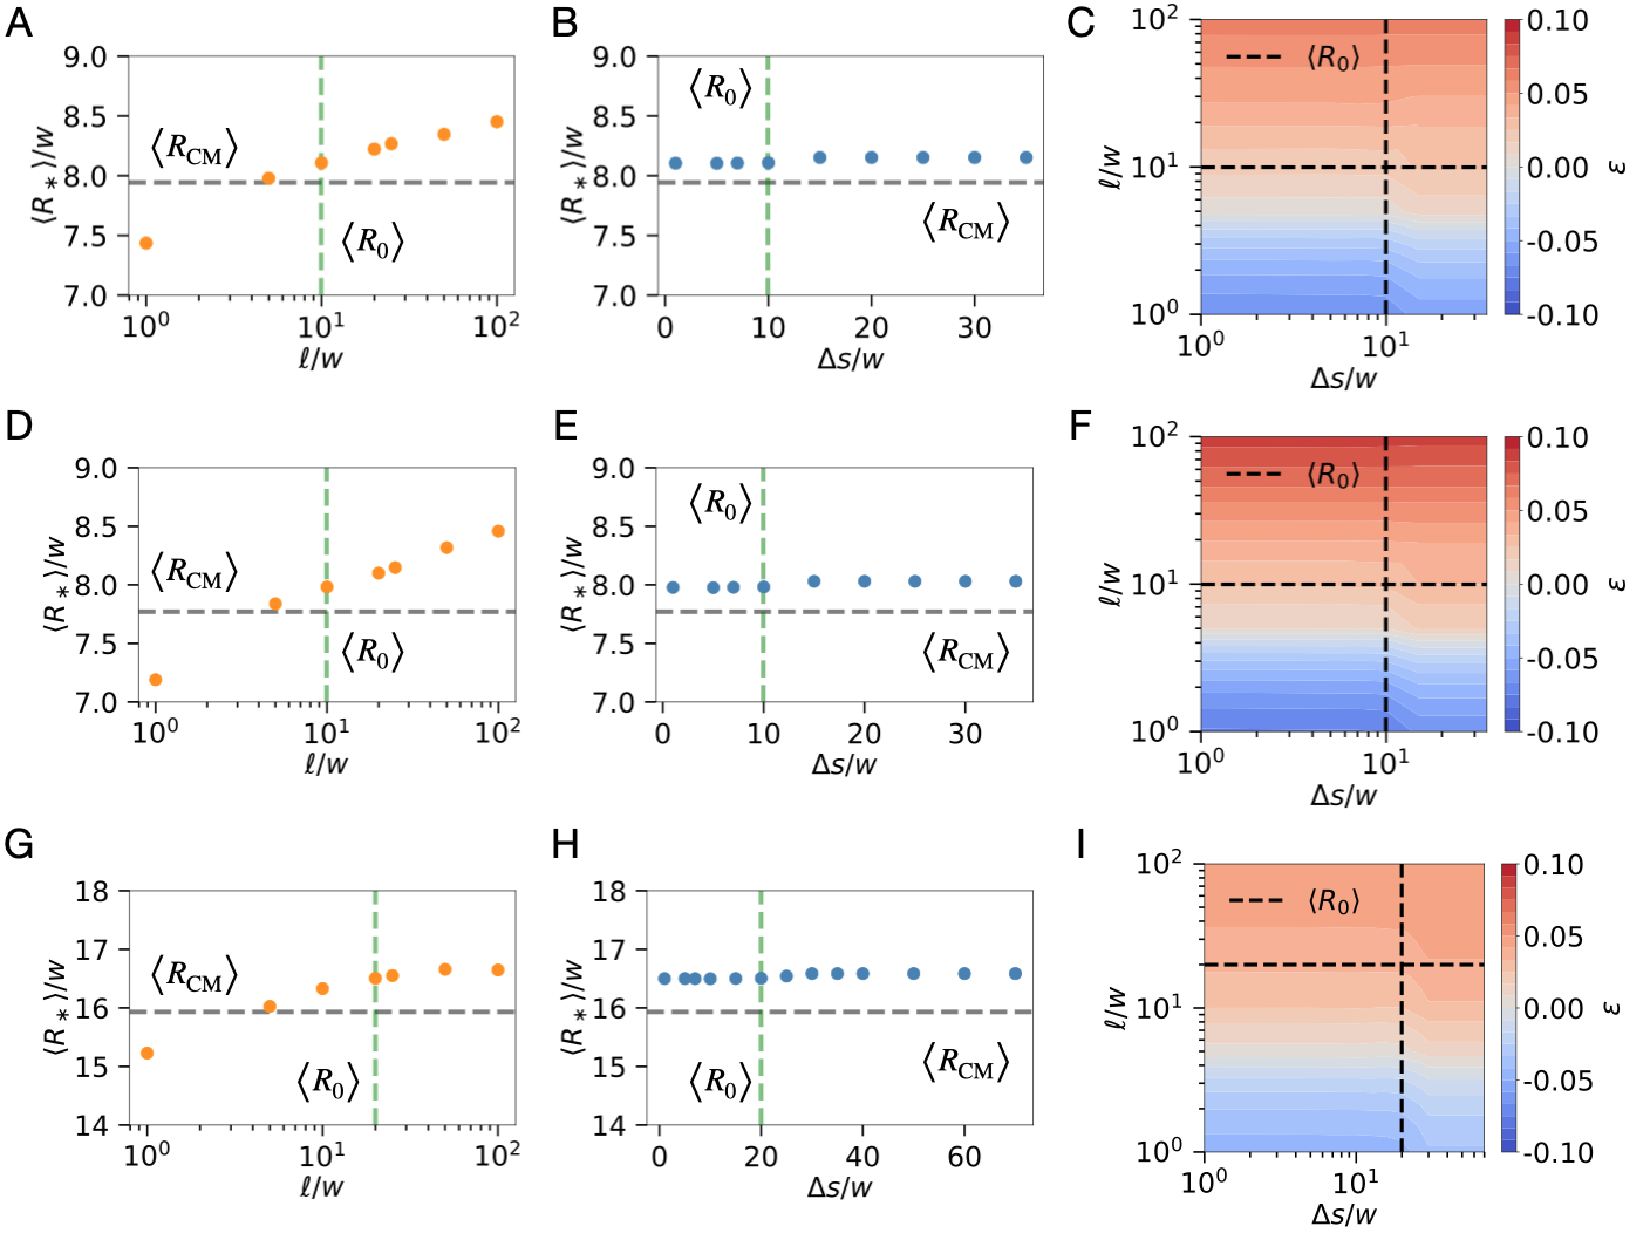
\includegraphics[scale=0.58]{MainContent/Figures/robustness_test_case.pdf}
\caption{\textbf{Effect of shell thickness $\ell$ and sector size $\ds$ on simulations of a passive droplet pair.}
\mbox{(A-C)} show simulations for the droplet pair when $[R_0, S_\mathrm{d}] = [10w, 40w]$.
(A) Mean droplet size $\langle R_\ast \rangle$ from the effective droplet model as a function of $\ell$ (orange dots) for $\dx \approx \ds \approx R_0$ compared to the ground truth $\mean{R_\mathrm{CM}}$ (gray dashed line) obtained from the continuous model.
The choice $\ell \approx R_0$ (green dashed line) provides good agreement and the error between $\left \langle R_\mathrm{CM} \right \rangle$ (dashed grey line) and $\left \langle R_\ast \right \rangle$ is less than $\pm 5\%$.
(B) $\langle R_\ast \rangle$ as a function of $\ds$ (blue dots) for $\dx \approx \ell \approx R_0$ compared to $\mean{R_\mathrm{CM}}$, where the error between $\left \langle R_\mathrm{CM} \right \rangle$ (dashed grey line) and $\left \langle R_\ast \right \rangle$ is less than $\pm 5\%$.
(C) Colorbar shows the error between the continuous model and the effective droplet model $\epsilon = [\langle R_\ast \rangle - \mean{R_\mathrm{CM}}] / \mean{R_\mathrm{CM}}$ is less than $\pm5\%$ for $\ds \approx \ell \approx R_0$.
\mbox{(D-F)} show simulations for the droplet pair when $[R_0, S_\mathrm{d}] = [10w, 100w]$.
\mbox{(G-I)} show simulations for the droplet pair when $[R_0, S_\mathrm{d}] = [20w, 80w]$.
We thus conclude that $\dx \approx \ds \approx \ell \approx R_0$ is the optimum choice for the simulation parameters for the effective droplet model. 
Remaining parameters are specified in Fig. \ref{fig:droplet_pair_schematics}.
}
\label{fig:robustness_test_case}
\end{figure}
Thus, from all the three different systems: $[R_0, S_\mathrm{d}] = [10w, 40w], [10w, 100w]$ and $[20w, 80w]$, we see that $\dx \approx \ds \approx \ell \approx R_0$ is a reasonable choice for the effective droplet model for which the error $\epsilon$ between the continuous model and the effective droplet model is less than $\pm 5\%$.

%%%%%%%%%%%%%%%%%%%%%%%%%%%%%%

\chapter{Droplet dynamics in external gradients in two dimensional systems}

\label{sec:droplet_gradient_2D}

Primarily, studies of phase separated condensates have mostly focused on three dimensional droplets. 
However, two dimensional phase separation is also relevant, for example, aggregation of shape regulating proteins; see Ref. \cite{gov2018} and emulsions in two dimensions; see Refs. \cite{Zwicker2015,Review2019,Bressloff_2020,Bressloff2020}.

We aim to demonstrate the effective model for a passive droplet in the presence of an external volume fraction gradient in two dimensional systems.
We compare the simulations using the effective droplet model with the continuous model and analytical predictions. 
Similar to a passive droplet in an external gradient in a three dimensional system; see Chapter \ref{chap:Chapter_5}, we first derive the droplet growth rate and drift speed for a passive droplet in an external volume fraction gradient in a large 2 dimensional system.

Consider an isolated passive droplet of radius $R \gg w$ with a polar co-ordinate
system centred at the droplet position $\vec{x_0}$.
The volume fraction outside the droplet can thus be expressed as $\phiOut(r, \theta)$, where $\theta \in [0, 2\pi]$. 
For simplicity, we again assume that the droplet experiences a one dimensional gradient that varies along the $x$-coordinate without loss of generality.
We utilize the framework of thin interface approximation and solve for the volume fraction profiles $\phiIn,~\phiOut$ inside and outside the droplet.
Since $\phiIn$ inside the droplet typically varies only a little, we use the thin-interface approximation and solve for $\phiIn$ from the steady state of \Eqref{eqn:RD_droplet_passive} using the boundary conditions $\phiIn(R) = \phiEqIn$ and $\partial_r \phiIn (0) = 0$ to obtain $\phiIn(r) = \phiEqIn$.

Similar to inside the droplet, the volume fraction inside in the background field $\phiOut$ also typically varies little can be solved from \Eqref{eqn:RD_droplet_passive} using the boundary conditions $\phi_\mathrm{out}(R) = \phiEq_\mathrm{out}$ and far from the droplet $\phi_\mathrm{out}(L) = \phi_{\infty} = \alpha + \beta \, L \, \text{cos}\,\theta$, where $L$ is the size of the large domain.
Note that since the volume fraction around the droplet varies as $\log(R)$, we do not consider truly infinite systems, but a large finite system of size $L$.
We thus obtain the volume fraction profile as 
\begin{equation*}
\phiOut(r, \theta) = \frac{\alpha - \frac {\phiEqOut \log(L) } { \log(R)}} { 1 - \frac{\log(L)}{\log(R)} } + \frac{\left ( \phiEqOut - \frac{\alpha - \frac {\phiEqOut \log(L) } {\log(R)}} { 1 - \frac{\log(L)}{\log(R)} } \right ) \log(r)}{\log(R)} + \left (\beta r - \frac{R^2 \beta}{r} \right ) \cos(\theta).
\end{equation*}
We now evaluate the local fluxes at the droplet surface similar to the approach used earlier as $\jIn = 0$,
\begin{equation*}
    \jOut \cdot \vec{n}= -D \left( 2 \beta \cos(\theta) +\frac{\left ( \phiEqOut - \frac{\alpha - \frac {\phiEqOut \log(L) } {\log(R)}} { 1 - \frac{\log(L)}{\log(R)} } \right )}{R \log R} \right ), 
\end{equation*}
and calculate the interfacial speed $v_n$ from \Eqref{eqn:InterfacialSpeed}.
We finally arrive at the droplet growth and drift speed from \Eqref{eqn:DropletGrowth} and \Eqref{eqn:DropletDrift} as

\begin{subequations}
\label{eqn:interfacefluxes_gradient_2D}
\begin{align}
	\frac{\mathrm{d} R}{\mathrm{d} t} &= \frac{1}{2 \pi} \int_{\Omega} D \left( 2 \beta \cos(\theta) +\frac{\left ( \phiEqOut - \frac{\alpha - \frac {\phiEqOut \log(L) } { \log(R)}} { 1 - \frac{\log(L)}{\log(R)} } \right )}{R \log R} \right ) \mathrm{d}A = \frac{D (\alpha - \phiEqOut)}{R \log \frac{L}{R}}
	\text{~and}
    \\[10pt]
    \frac{\mathrm{d} x_0}{\mathrm{d} t} &= \frac{1}{\pi} \int_{\Omega} D \left( 2 \beta \cos(\theta) +\frac{\left ( \phiEqOut - \frac{\alpha - \frac {\phiEqOut \log(L) } {\log(R)}} { 1 - \frac{\log(L)}{\log(R)} } \right )}{R \log R} \right ) \cos(\theta) \, \mathrm{d}A = 2 D \beta,
\end{align}
\end{subequations}
where $D$ is the diffusivity, $L$ is the system size, $R$ is the droplet radius, $\Omega$ is the droplet surface and $\mathrm{d} A$ is the area element on the droplet surface.

\begin{figure}[t]
\centering
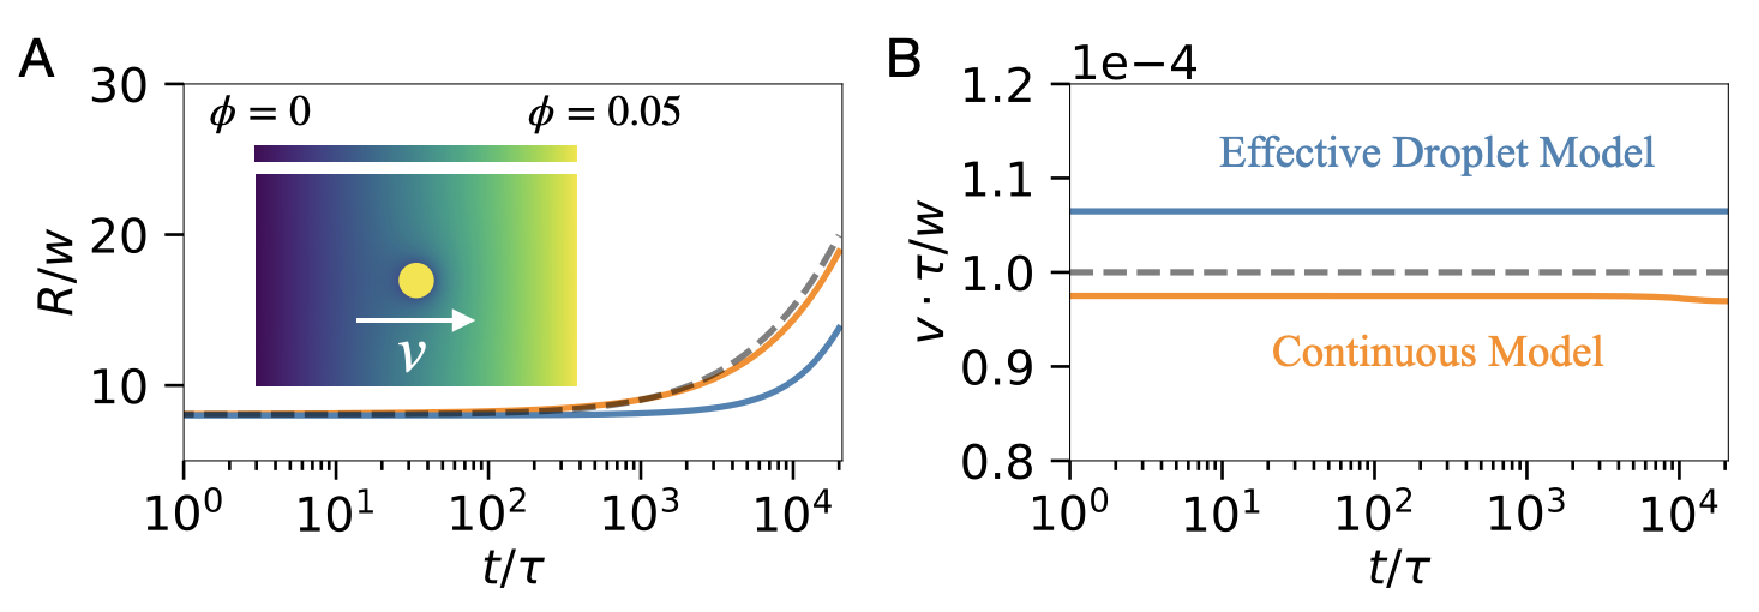
\includegraphics[scale=0.5]{MainContent/Figures/Strong_Gradient_2D.pdf}
\caption{\textbf{Droplet dynamics in external gradients in two dimensional systems.}
(A) Droplet radius $R$ as a function of time $t$ from the effective droplet model (blue), analytical prediction (dashed line) from \Eqsref{eqn:interfacefluxes_gradient_2D} and the continuous model (orange).
The inset shows a schematic of the simulation with the imposed gradient of droplet material.
(B) Droplet drift speed $v$ as function of $t$ using the effective droplet model (blue) and the analytical prediction (dashed line) from \Eqsref{eqn:interfacefluxes_gradient_2D}, with simulations using the continuous model (orange).
\mbox{(A, B)}
The continuous and the effective droplet model uses a Cartesian 2 dimensional domain with $x,y \in [-L, L]$, with $L=500 w$. The boundary conditions are $\mu(x=-L) = 0$ and $\mu(x=L)= 0.0427\,b\,w^2$ for the continuous model and $\phiOut(x=-L) = 0$ and $\phiOut(x=L)= 0.05$ to maintain the gradient throughout the system.
The effective model uses $\dx \approx \ell \approx \Delta s \approx R_0$.
Note that in the absence of droplets, boundary conditions imply identical linear gradient in the effective droplet model as $\phi=\phi(x)$ and in the continuous model as $\phiOut=\phiOut(x)$, which were also used to initialize the background for both the models.
Remaining parameters are specified in Fig. \ref{fig:droplet_pair_schematics}.
}
\label{fig:drop_in_gradient_2D}
\end{figure}

We simulate a single passive droplet of initial radius $R_0 = 6w$ immersed in a linear volume fraction gradient of the droplet material. 
Similar to the case of the passive droplet growing in a supersaturated medium, the passive droplet in this case also grows over time by taking material from the surroundings. 
Furthermore, as $\jOut \cdot \vec{n}$ has an angular dependence, it results in unequal fluxes leading to droplet drift along the gradient.
The continuous and the effective droplet model use a Cartesian two dimensional domain with $x,y \in [-L, L]$, with $L=500 w$. 
The boundary conditions are $\mu(x=-L) = 0$ and $\mu(x=L)= 0.0427\,b\,w^3$ for the continuous model and $\phiOut(x=-L) = 0$ and $\phiOut(x=L)= 0.05$ to maintain the gradient throughout the system.
The effective model uses $\dx \approx \ell \approx \Delta s \approx R_0$.
\figref{fig:drop_in_gradient_2D} shows droplet growth and drift speed using the effective droplet model with optimum parameters ($\dx \approx \ell \approx \Delta s \approx R_0$), simulations using the continuous model and analytical predictions from \Eqsref{eqn:interfacefluxes_gradient_2D}.

%%%%%%%%%%%%%%%%%%%%%%%%%%%%%%%%

\end{appendices}
\clearpage

% References
%========================================

\addcontentsline{toc}{chapter}{Bibliography}
\begin{singlespace}
	\setlength\bibitemsep{\baselineskip}
	\printbibliography[title={Bibliography}]
\end{singlespace}

\end{document}
